%!TEX root = ../main.tex
\chapter{Campo Elettrostatico}

In questa sezione assumeremo che gli oggetti interagenti si muovano seguendo le leggi della meccanica classica. I fenomeni elettrostatici sono quelli di natura elettrica in cui gli oggetti sono in quiete in un sistema di riferimento inerziale. Essi sono noti fin dall'antichità. In greco antico l'ambra si chiama elecrton, da qui deriva il termine elettricità. I fenomeni elettrici sono rimasti per molti secoli una curiosità fino al 1600 in cui vi è la corsa allo studio dei pianeti. Cominciano ad esserci su di essi tutta una serie di teorie fra cui quelle sull'esistenza delle forze di tipo elettrico o magnetico. La teoria cadde in disuso dopo le scoperte di Newton sulla gravitazione universale. Nel corso del 1700 tuttavia incominciano tutta una serie di esperienze. Nel 1740 si scopre che gli oggetti si dividono in isolanti e conduttori. Dieci anni dopo si scopre il concetto di carica elettrica. Nel 1785 Coulomb si accorge che c'è una legge generale che regola l'interazione fra cariche elettriche. Nel 1800 volta inventa la pila elettrica. Grazie a tale oggetto si cominciano a studiare i fenomeni della conduzione elettrica. Faraday studia anche le leggi dell'elettrolisi; in particolare, in una cella elettrolitica la massa depositata fra gli elettrodi è proporzionale alla quantità di carica che ha attraversato la cella. Nel 1917 ha luogo l'esperimento di Millikan, sulla quantizzazione carica elettrica.

\section{Struttura della materia}

La materia così come la conosciamo si compone di tre particelle: \textbf{protoni neutroni ed elettroni}. Per quanto riguarda protoni e neutroni, la loro massa è $m_p \sim m_n \sim  1.67 \times 10^{-27} \text{kg}$.
La massa dell'elettrone è quella del protone divisa per 1840: $m_e= \frac{m_p}{1840}=9,1\times 10^{31} \text{kg}$.
Si pensa che le dimensioni del protone e neutrone siano dell'ordine del pentometro, $10^{-15}\,m$.
Protoni e neutroni sono particelle passive a loro volta composte da sub-particelle. I protoni sono dotati anche di carica elettrica. In particolare tale carica è positiva e viene indicata con la lettera $e=1.6\times 10^{-19} C$.
La carica elettrica dell'elettrone invece è pari a $-e$. Si tratta di cariche di segno opposto. La cosa da notare è che siccome queste sono le particelle più piccole che caratterizzano la materia, le cariche estratte non possono che essere multipli fondamentali di $e$. La carica elettrica per tale motivo pare essere quantizzata. Cariche più piccole non sono mai state osservate in natura, anche se sappiamo che protoni e neutroni sono composti da particelle ancora più piccole, i quark, aventi carica elettrica stazionaria. Il neutrone è privo di carica.
L'elettromagnetismo governa le interazioni fra elettrone e nucleo. La struttura dell'atomo è quella di un nucleo positivo in cui abbiamo protoni e neutroni legati fra loro da interazioni nucleari forti, attorno al quale orbitano elettroni di carica negativa. Nello stato fondamentale un atomo è sempre elettricamente neutro. Ciò significa che la somma algebrica delle cariche contenute al suo interno fa $0$. Il numero di elettroni e di protoni è lo stesso. Il numero atomico, ossia il numero di protoni, è quello che ne stabilisce le proprietà chimiche.
Il numero di massa è la somma del numero di protoni più quello di neutroni.
Possiamo avere atomi con stesso numero atomico ma diverso numero di massa, si parla di isotopi. La cosa fondamentale è che l'atomo è sempre neutro. Le dimensioni dell'atomo sono dell'ordine di $10^{-10}\,m = 1 $ Angstrom e sono 100mila volte maggiori di quelle del nucleo. Esso è piccolissimo ed è circondato da una nube di elettroni che si muovono in uno spazio sostanzialmente vuoto.

\subsection{Principio di conservazione della carica elettrica}

Afferma che considerato un sistema isolato la \emph{somma algebrica di tutte le cariche} in esso presenti rimane costante nel tempo, ovvero \emph{si conserva}. Tale principio lo si può comprendere in base a come è strutturata la materia. Se abbiamo un sistema isolato in cui non c'è scambio di massa al suo interno il numero di elettroni e protoni rimane costante nel tempo. Dal punto di vista della fisica classica corrisponde al principio di conservazione della massa.

\subsection{Fenomeni triboelettrici}

I fenomeni triboelettrici sono quei fenomeni indotti per strofinio. Se prendiamo due oggetti e li strofiniamo per poi metterli in prossimità, essi cominciano a interagire tramite un interazione che ha le seguenti proprietà:

\begin{itemize}
	\item Le forze sono di tipo repulsivo se gli oggetti sono dello stesso materiale.
	\item Altrimenti, a seconda delle sostanze con cui sono fatti gli oggetti osserveremo forze di tipo attrattivo o repulsivo. Se considero un panno di lana e un altro oggetto vi è sempre interazione di tipo attrattivo.
	\item Se consideriamo tre oggetti noteremo che se $A$ e $C$ si attraggono e $C$ e $B$ si attraggono, allora $A$ e $B$ si respingono. Viceversa se $A$ e $C$ ed $B$ e $C$ si respingono, $A$ e $B$ si attraggono.
\end{itemize}

Osserviamo cariche elettriche positive e negative. Quello che deduciamo sperimentalmente è che cariche dello stesso segno si respingono e cariche di segno opposto si attraggono. Mentre le forze gravitazionali sono solo attrattive, quelle elettrostatiche sono sia attrattive che repulsive.
Dopo lo strofinio ci troveremo in uno stato di elettrizzazione. Le cariche nucleari non sono più completamente compensate. Consideriamo un materiale composto da plastica. Avremo un trasferimento di elettroni dal panno alla plastica, essi di attraggono. In generale questi fenomeni sono dovuti al trasferimento di carica elettrica. Tutti i materiali citati sono detti isolanti o dielettrici. Quando strofino un materiale isolante otterrò in quel punto un eccesso di carica ma essa non si distribuisce, rimane localizzata in quel punto. In tali materiali c'è una scarsa mobilità delle cariche elettriche.
Esiste anche una grande categoria di materiali detti conduttori. Tipicamente essi sono materiali metallici. Ciò che accade è che alcuni elettroni dei vari atomi sono messi in compartecipazione e liberi di muoversi. Possiamo immaginare che ci sia un gas di elettroni liberi. Se depongo della carica negativa in un certo punto essa su sposta immediatamente e si ridistribuisce su tutto il materiale.

È sperimentalmente dimostrato che se consideriamo un conduttore inizialmente neutro e vi avviciniamo una carica elettrica, proprio perché al suo interno le cariche sono libere di muoversi fra loro, gli elettroni si affacceranno su un lato. Le cariche sono sempre le stesse ma sono separate. Questo fenomeno prende il nome di induzione elettrica. Se colleghiamo il conduttore con un filo ad un conduttore molto più grande, ad esempio il pianeta terra, là cariche positive, siccome sono libere di muoversi e si respingono fra loro, vogliono disporsi in modo più lontano possibile l'una dall'altra e quindi fuggono verso terra.

\section{Legge di Coulomb}

È stato Coulomb a iniziare a studiare in maniera sistematica le cariche elettriche e le interazioni fra oggetti carichi elettricamente di dimensioni trascurabili rispetto alla distanza fra di loro. Egli è arrivato a formulare una legge che vale solo quindi per quanto riguarda le cariche puntiformi.

\begin{figure}[htpb]
	\centering

	\tikzset{every picture/.style={line width=0.75pt}} %set default line width to 0.75pt        

	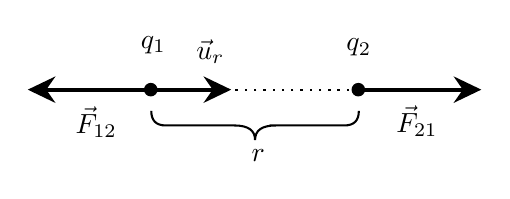
\begin{tikzpicture}[x=0.75pt,y=0.75pt,yscale=-1,xscale=1]
	%uncomment if require: \path (0,300); %set diagram left start at 0, and has height of 300

	%Shape: Circle [id:dp6759441700488122] 
	\draw  [fill={rgb, 255:red, 0; green, 0; blue, 0 }  ,fill opacity=1 ] (120,123.75) .. controls (120,122.23) and (121.23,121) .. (122.75,121) .. controls (124.27,121) and (125.5,122.23) .. (125.5,123.75) .. controls (125.5,125.27) and (124.27,126.5) .. (122.75,126.5) .. controls (121.23,126.5) and (120,125.27) .. (120,123.75) -- cycle ;
	%Straight Lines [id:da770733030940054] 
	\draw [line width=1.5]    (122.75,123.75) -- (67.5,123.75) ;
	\draw [shift={(63.5,123.75)}, rotate = 360] [fill={rgb, 255:red, 0; green, 0; blue, 0 }  ][line width=0.08]  [draw opacity=0] (13.4,-6.43) -- (0,0) -- (13.4,6.44) -- (8.9,0) -- cycle    ;
	%Shape: Circle [id:dp8565834305540732] 
	\draw  [fill={rgb, 255:red, 0; green, 0; blue, 0 }  ,fill opacity=1 ] (220,123.75) .. controls (220,122.23) and (221.23,121) .. (222.75,121) .. controls (224.27,121) and (225.5,122.23) .. (225.5,123.75) .. controls (225.5,125.27) and (224.27,126.5) .. (222.75,126.5) .. controls (221.23,126.5) and (220,125.27) .. (220,123.75) -- cycle ;
	%Straight Lines [id:da7726897544624338] 
	\draw [line width=1.5]    (278,123.75) -- (222.75,123.75) ;
	\draw [shift={(282,123.75)}, rotate = 180] [fill={rgb, 255:red, 0; green, 0; blue, 0 }  ][line width=0.08]  [draw opacity=0] (13.4,-6.43) -- (0,0) -- (13.4,6.44) -- (8.9,0) -- cycle    ;
	%Straight Lines [id:da33333178128062513] 
	\draw [line width=1.5]    (157.5,123.75) -- (122.75,123.75) ;
	\draw [shift={(161.5,123.75)}, rotate = 180] [fill={rgb, 255:red, 0; green, 0; blue, 0 }  ][line width=0.08]  [draw opacity=0] (13.4,-6.43) -- (0,0) -- (13.4,6.44) -- (8.9,0) -- cycle    ;
	%Straight Lines [id:da5435846648051312] 
	\draw [line width=0.75]  [dash pattern={on 0.84pt off 2.51pt}]  (222.75,123.75) -- (122.75,123.75) ;
	%Shape: Brace [id:dp15876881438202872] 
	\draw   (123,134) .. controls (123,138.67) and (125.33,141) .. (130,141) -- (163,141) .. controls (169.67,141) and (173,143.33) .. (173,148) .. controls (173,143.33) and (176.33,141) .. (183,141)(180,141) -- (216,141) .. controls (220.67,141) and (223,138.67) .. (223,134) ;

	% Text Node
	\draw (124,102.5) node    {$q_{1}$};
	% Text Node
	\draw (223,103.5) node    {$q_{2}$};
	% Text Node
	\draw (251,139) node    {$\vec{F}_{21}$};
	% Text Node
	\draw (96.5,139.5) node    {$\vec{F}_{12}$};
	% Text Node
	\draw (151.5,105.5) node    {$\vec{u}_{r}$};
	% Text Node
	\draw (174.5,155.5) node    {$r$};

	\end{tikzpicture}
\end{figure}
\FloatBarrier

Siano due cariche in quiete in un sistema di riferimento inerziale. Sia $r$ la distanza fra le cariche. $\vec{F}_{21}$ può essere scritta come:

\[
	\boxed{\vec{F}_{21}=k \frac{q_1q_2}{r^2} \vec{u}_r}  \qquad \text{con} \quad k=8.98\times 10^9 \, Nm^2 /C^2
\]

Con $\vec{u}_r$ versore radiale. Tale legge ricorda quella di gravitazione universale di Newton.

\[
	\vec{F}_{12}=-\vec{F}_{21}
\]

Guardiamo $\vec{F}_{21}$ come funzione vettoriale della posizione, che associa ad un punto dello spazio il vettore forza. Abbiamo così identificato un campo vettoriale. La Nostra forza $\vec{F}_{21}$ è un campo vettoriale il cui modulo dipende solo dalla distanza $r$ e la cui direzione è quella radiale. Si parla di \textbf{campo di forza centrale}. Si può dimostrare che un campo di forza centrale è \emph{conservativo}. Per le proprietà introdotte, il verso della forza è opposto a $\vec{u}_r$ se le cariche sono opposte. La legge di Coulomb contiene in questo senso già tutti i casi possibili.

Vediamo una seconda versione. Immaginiamo di identificare la posizione di $q_2$ rispetto a $q_1$ con un vettore posizione $r$. Il versore $\vec{u}_r$ si può anche scrivere come il rapporto:

\[
	\frac{\vec{r}}{|\vec{r} |} = \frac{\vec{r}}{r}
\]

Poniamoci in un sistema di coordinate cartesiane.

\begin{figure}[htpb]
	\centering

	\tikzset{every picture/.style={line width=0.75pt}} %set default line width to 0.75pt        

	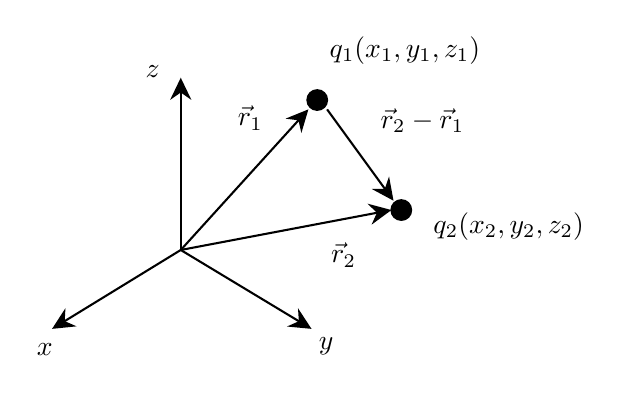
\begin{tikzpicture}[x=0.75pt,y=0.75pt,yscale=-1,xscale=1]
	%uncomment if require: \path (0,300); %set diagram left start at 0, and has height of 300

	%Straight Lines [id:da6964491635777041] 
	\draw    (179.5,140) -- (179.5,60) ;
	\draw [shift={(179.5,57)}, rotate = 450] [fill={rgb, 255:red, 0; green, 0; blue, 0 }  ][line width=0.08]  [draw opacity=0] (10.72,-5.15) -- (0,0) -- (10.72,5.15) -- (7.12,0) -- cycle    ;
	%Straight Lines [id:da7452549937508859] 
	\draw    (179.5,140) -- (239.93,176.45) ;
	\draw [shift={(242.5,178)}, rotate = 211.1] [fill={rgb, 255:red, 0; green, 0; blue, 0 }  ][line width=0.08]  [draw opacity=0] (10.72,-5.15) -- (0,0) -- (10.72,5.15) -- (7.12,0) -- cycle    ;
	%Straight Lines [id:da5024739469391739] 
	\draw    (179.5,140) -- (120.06,176.43) ;
	\draw [shift={(117.5,178)}, rotate = 328.5] [fill={rgb, 255:red, 0; green, 0; blue, 0 }  ][line width=0.08]  [draw opacity=0] (10.72,-5.15) -- (0,0) -- (10.72,5.15) -- (7.12,0) -- cycle    ;
	%Shape: Circle [id:dp27933265319891487] 
	\draw  [fill={rgb, 255:red, 0; green, 0; blue, 0 }  ,fill opacity=1 ] (240.5,67.75) .. controls (240.5,65.13) and (242.63,63) .. (245.25,63) .. controls (247.87,63) and (250,65.13) .. (250,67.75) .. controls (250,70.37) and (247.87,72.5) .. (245.25,72.5) .. controls (242.63,72.5) and (240.5,70.37) .. (240.5,67.75) -- cycle ;
	%Shape: Circle [id:dp5790263105950524] 
	\draw  [fill={rgb, 255:red, 0; green, 0; blue, 0 }  ,fill opacity=1 ] (281,120.75) .. controls (281,118.13) and (283.13,116) .. (285.75,116) .. controls (288.37,116) and (290.5,118.13) .. (290.5,120.75) .. controls (290.5,123.37) and (288.37,125.5) .. (285.75,125.5) .. controls (283.13,125.5) and (281,123.37) .. (281,120.75) -- cycle ;
	%Straight Lines [id:da3756037875902982] 
	\draw    (179.5,140) -- (238.98,74.47) ;
	\draw [shift={(241,72.25)}, rotate = 492.23] [fill={rgb, 255:red, 0; green, 0; blue, 0 }  ][line width=0.08]  [draw opacity=0] (10.72,-5.15) -- (0,0) -- (10.72,5.15) -- (7.12,0) -- cycle    ;
	%Straight Lines [id:da6433495966928404] 
	\draw    (179.5,140) -- (278.05,121.31) ;
	\draw [shift={(281,120.75)}, rotate = 529.26] [fill={rgb, 255:red, 0; green, 0; blue, 0 }  ][line width=0.08]  [draw opacity=0] (10.72,-5.15) -- (0,0) -- (10.72,5.15) -- (7.12,0) -- cycle    ;
	%Straight Lines [id:da4508868053914086] 
	\draw    (250,72.25) -- (280.24,113.82) ;
	\draw [shift={(282,116.25)}, rotate = 233.97] [fill={rgb, 255:red, 0; green, 0; blue, 0 }  ][line width=0.08]  [draw opacity=0] (10.72,-5.15) -- (0,0) -- (10.72,5.15) -- (7.12,0) -- cycle    ;

	% Text Node
	\draw (114,188) node    {$x$};
	% Text Node
	\draw (249.5,186.5) node    {$y$};
	% Text Node
	\draw (166,54) node    {$z$};
	% Text Node
	\draw (296,77.5) node    {$\vec{r}_{2} -\vec{r}_{1}$};
	% Text Node
	\draw (258,142.5) node    {$\vec{r}_{2}$};
	% Text Node
	\draw (213,76.5) node    {$\vec{r}_{1}$};
	% Text Node
	\draw (287.5,44) node    {$q_{1}( x_{1} ,y_{1} ,z_{1})$};
	% Text Node
	\draw (337.5,128.5) node    {$q_{2}( x_{2} ,y_{2} ,z_{2})$};

	\end{tikzpicture}
\end{figure}
\FloatBarrier

\begin{gather*}
	\vec{r}_1 = x_1\vec{u}_x+y_1\vec{u}_y+z_1\vec{u}_z \\
	\vec{r}_2 = x_2\vec{u}_x+y_2\vec{u}_y+z_2\vec{u}_z \\
	\vec{F}_{21} = k q_1q_2 \frac{\vec{r}_1-\vec{r}_2}{|r_1-r_2  |^3}
\end{gather*}

Fino al 2018 la grandezza fondamentale era l'intensità di corrente. Formalmente nel sistema internazionale le dimensioni della carica sono quelle della corrente per un tempo.

\[
	[Q] = [I][T] = (A\cdot s) = C \quad \text{Coulomb}
\]

Dal 2019 si assume che la carica dell'elettrone sia esattamente pari a $1.60 \times 10^{-19} C$ e da qui si definisce il Coulomb. Le forze elettriche come vediamo dal valore di k sono forze estremamente intense. In realtà k spesso viene descritta come:

\[
	k=\frac{1}{4\pi \varepsilon_0}
\]
$\varepsilon_0$ è la \textbf{costante elettrica assoluta del vuoto}. Il suo valore è $\varepsilon_0 = 8.85 \times 10^{-12} C^2 / N m^2$.
A livello microscopico le forze gravitazionali non contano nulla. Se infatti proviamo a mettere a confronto l'intensità della forza di Coulomb e della forza gravitazionale calcolate relativamente all'atomo di idrogeno, si ha:

\[
	F_e = \frac{e^2}{4\pi \varepsilon_0 r^2} = 9\times 10^8N \qquad F_G = \frac{G m_p m_e}{r^2}   =4\times 10^{-47} N
\]

\begin{figure}[htpb]
	\centering

	\tikzset{every picture/.style={line width=0.75pt}} %set default line width to 0.75pt        

	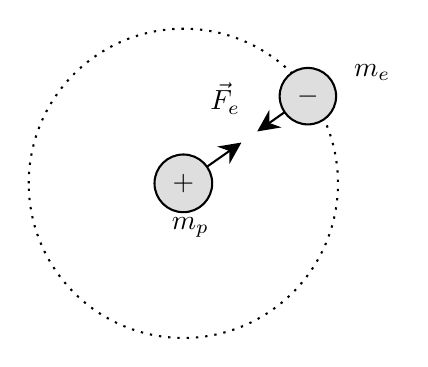
\begin{tikzpicture}[x=0.75pt,y=0.75pt,yscale=-1,xscale=1]
	%uncomment if require: \path (0,300); %set diagram left start at 0, and has height of 300

	%Shape: Circle [id:dp9391076515585639] 
	\draw  [dash pattern={on 0.84pt off 2.51pt}] (182.5,133) .. controls (182.5,91.85) and (215.85,58.5) .. (257,58.5) .. controls (298.15,58.5) and (331.5,91.85) .. (331.5,133) .. controls (331.5,174.15) and (298.15,207.5) .. (257,207.5) .. controls (215.85,207.5) and (182.5,174.15) .. (182.5,133) -- cycle ;
	%Straight Lines [id:da7327286186495761] 
	\draw    (295.04,106.28) -- (318.2,90) ;
	\draw [shift={(292.58,108)}, rotate = 324.91] [fill={rgb, 255:red, 0; green, 0; blue, 0 }  ][line width=0.08]  [draw opacity=0] (10.72,-5.15) -- (0,0) -- (10.72,5.15) -- (7.12,0) -- cycle    ;
	%Straight Lines [id:da28216679196328576] 
	\draw    (257,133) -- (282.55,115.05) ;
	\draw [shift={(285,113.33)}, rotate = 504.91] [fill={rgb, 255:red, 0; green, 0; blue, 0 }  ][line width=0.08]  [draw opacity=0] (10.72,-5.15) -- (0,0) -- (10.72,5.15) -- (7.12,0) -- cycle    ;

	% Text Node
	\draw  [fill={rgb, 255:red, 222; green, 222; blue, 222 }  ,fill opacity=1 ]  (257, 133) circle [x radius= 13.9, y radius= 13.9]   ;
	\draw (257,133) node    {$+$};
	% Text Node
	\draw  [fill={rgb, 255:red, 222; green, 222; blue, 222 }  ,fill opacity=1 ]  (317, 91) circle [x radius= 13.6, y radius= 13.6]   ;
	\draw (317,91) node    {$-$};
	% Text Node
	\draw (260.4,154.2) node    {$m_{p}$};
	% Text Node
	\draw (348,79.8) node    {$m_{e}$};
	% Text Node
	\draw (277.2,92.2) node    {$\vec{F}_{e}$};

	\end{tikzpicture}
\end{figure}
\FloatBarrier

\section{Principio di sovrapposizione}

Fondamentale in questo campo è il principio di sovrapposizione degli effetti. In matematica e in fisica, il \textbf{principio di sovrapposizione} stabilisce che per un sistema dinamico lineare l'effetto di una somma di perturbazioni in ingresso è uguale alla somma degli effetti prodotti da ogni singola perturbazione. Il principio di sovrapposizione esprime la possibilità di scomporre un problema lineare.

\begin{figure}[htpb]
	\centering

	\tikzset{every picture/.style={line width=0.75pt}} %set default line width to 0.75pt        

	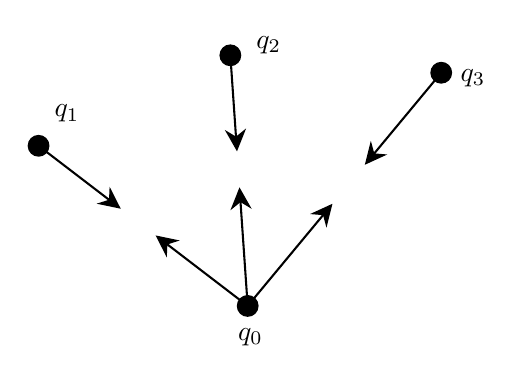
\begin{tikzpicture}[x=0.75pt,y=0.75pt,yscale=-1,xscale=1]
	%uncomment if require: \path (0,300); %set diagram left start at 0, and has height of 300

	%Shape: Circle [id:dp9532587092519822] 
	\draw  [fill={rgb, 255:red, 0; green, 0; blue, 0 }  ,fill opacity=1 ] (206.6,229.15) .. controls (206.6,226.53) and (208.73,224.4) .. (211.35,224.4) .. controls (213.97,224.4) and (216.1,226.53) .. (216.1,229.15) .. controls (216.1,231.77) and (213.97,233.9) .. (211.35,233.9) .. controls (208.73,233.9) and (206.6,231.77) .. (206.6,229.15) -- cycle ;
	%Straight Lines [id:da6293871325411147] 
	\draw    (269.72,158.83) -- (304.6,116.8) ;
	\draw [shift={(267.8,161.14)}, rotate = 309.69] [fill={rgb, 255:red, 0; green, 0; blue, 0 }  ][line width=0.08]  [draw opacity=0] (10.72,-5.15) -- (0,0) -- (10.72,5.15) -- (7.12,0) -- cycle    ;
	%Shape: Boxed Line [id:dp10731073492947596] 
	\draw    (147.82,180.5) -- (110.6,152) ;
	\draw [shift={(150.2,182.32)}, rotate = 217.44] [fill={rgb, 255:red, 0; green, 0; blue, 0 }  ][line width=0.08]  [draw opacity=0] (10.72,-5.15) -- (0,0) -- (10.72,5.15) -- (7.12,0) -- cycle    ;
	%Shape: Boxed Line [id:dp7675257187319859] 
	\draw    (205.99,151.68) -- (203,108.4) ;
	\draw [shift={(206.2,154.68)}, rotate = 266.04] [fill={rgb, 255:red, 0; green, 0; blue, 0 }  ][line width=0.08]  [draw opacity=0] (10.72,-5.15) -- (0,0) -- (10.72,5.15) -- (7.12,0) -- cycle    ;
	%Shape: Circle [id:dp9186357505606382] 
	\draw  [fill={rgb, 255:red, 0; green, 0; blue, 0 }  ,fill opacity=1 ] (299.85,116.8) .. controls (299.85,114.18) and (301.98,112.05) .. (304.6,112.05) .. controls (307.22,112.05) and (309.35,114.18) .. (309.35,116.8) .. controls (309.35,119.42) and (307.22,121.55) .. (304.6,121.55) .. controls (301.98,121.55) and (299.85,119.42) .. (299.85,116.8) -- cycle ;
	%Shape: Circle [id:dp6102120191986977] 
	\draw  [fill={rgb, 255:red, 0; green, 0; blue, 0 }  ,fill opacity=1 ] (198.25,108.4) .. controls (198.25,105.78) and (200.38,103.65) .. (203,103.65) .. controls (205.62,103.65) and (207.75,105.78) .. (207.75,108.4) .. controls (207.75,111.02) and (205.62,113.15) .. (203,113.15) .. controls (200.38,113.15) and (198.25,111.02) .. (198.25,108.4) -- cycle ;
	%Shape: Circle [id:dp9249207905796555] 
	\draw  [fill={rgb, 255:red, 0; green, 0; blue, 0 }  ,fill opacity=1 ] (105.85,152) .. controls (105.85,149.38) and (107.98,147.25) .. (110.6,147.25) .. controls (113.22,147.25) and (115.35,149.38) .. (115.35,152) .. controls (115.35,154.62) and (113.22,156.75) .. (110.6,156.75) .. controls (107.98,156.75) and (105.85,154.62) .. (105.85,152) -- cycle ;
	%Shape: Boxed Line [id:dp3327031648527261] 
	\draw    (211.35,229.15) -- (169.38,197.01) ;
	\draw [shift={(167,195.19)}, rotate = 397.44] [fill={rgb, 255:red, 0; green, 0; blue, 0 }  ][line width=0.08]  [draw opacity=0] (10.72,-5.15) -- (0,0) -- (10.72,5.15) -- (7.12,0) -- cycle    ;
	%Shape: Boxed Line [id:dp8962126358308287] 
	\draw    (211.35,229.15) -- (207.61,175.02) ;
	\draw [shift={(207.4,172.03)}, rotate = 446.04] [fill={rgb, 255:red, 0; green, 0; blue, 0 }  ][line width=0.08]  [draw opacity=0] (10.72,-5.15) -- (0,0) -- (10.72,5.15) -- (7.12,0) -- cycle    ;
	%Shape: Boxed Line [id:dp2779968769324759] 
	\draw    (211.35,229.15) -- (250.28,182.24) ;
	\draw [shift={(252.2,179.93)}, rotate = 489.69] [fill={rgb, 255:red, 0; green, 0; blue, 0 }  ][line width=0.08]  [draw opacity=0] (10.72,-5.15) -- (0,0) -- (10.72,5.15) -- (7.12,0) -- cycle    ;

	% Text Node
	\draw (221.5,103.7) node    {$q_{2}$};
	% Text Node
	\draw (212.7,244.1) node    {$q_{0}$};
	% Text Node
	\draw (319.9,119.3) node    {$q_{3}$};
	% Text Node
	\draw (124.3,136.5) node    {$q_{1}$};

	\end{tikzpicture}
\end{figure}
\FloatBarrier

Se si è in grado di scrivere i dati di ingresso in più componenti linearmente indipendenti (ad esempio, in un moto a due dimensioni si possono considerare la componente verticale e la componente orizzontale) allora è possibile risolvere il problema analizzando separatamente ciascuna delle componenti: si calcola ogni singola risposta e poi si sommano le singole risposte secondo la stessa proporzione (ovvero con gli stessi coefficienti).

\[
	\vec{R} = \Sigma_i\vec{F}_i  =\Sigma_i \frac{q_iq}{4\pi \varepsilon_0 r_i^2} \vec{u}_{r_i}
\]

Così arriviamo a dire che per le forze, la risultante delle forze è la somma delle varie forze che ciascuna delle cariche esercita da sola sulla carica in questione.

\section{Campo Elettrico}

Molto spesso le interazioni di tipo elettrico non vengono trattate in termini di forza ma sono interpretate in un altro modo.
Consideriamo il caso della coppia di cariche $Q$ e $q$ e chiamiamo $P$ la posizione della carica $q$. La forza $\vec{F}$ dipende dalla posizione della carica. L'espressione rappresentata dalla legge di Coulomb associa ad ogni punto dello spazio un vettore, si parla di campo vettoriale.
Potremmo interpretare la forza nel seguente modo. Immaginiamo di avere $Q$ isolata dal resto dell'universo. Possiamo immaginare che la sua presenza alteri le proprietà dello spazio circostante. Questa alterazione non è visibile fino a che non avviciniamo un'altra carica. Chiameremo la $Q$ sorgente e la $q$ esploratrice. L'alterazione della sorgente è visibile solo in presenza di una carica esploratrice, che diventa un modo per sondare tale effetto. Invece di vedere le alterazioni come fra due oggetti che hanno la stessa dignità, ci concentriamo sugli effetti di uno sull'altro.

\begin{figure}[htpb]
	\centering

	\tikzset{every picture/.style={line width=0.75pt}} %set default line width to 0.75pt        

	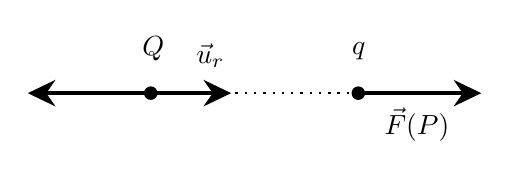
\begin{tikzpicture}[x=0.75pt,y=0.75pt,yscale=-1,xscale=1]
	%uncomment if require: \path (0,300); %set diagram left start at 0, and has height of 300

	%Shape: Circle [id:dp1923816477548197] 
	\draw  [fill={rgb, 255:red, 0; green, 0; blue, 0 }  ,fill opacity=1 ] (140,143.75) .. controls (140,142.23) and (141.23,141) .. (142.75,141) .. controls (144.27,141) and (145.5,142.23) .. (145.5,143.75) .. controls (145.5,145.27) and (144.27,146.5) .. (142.75,146.5) .. controls (141.23,146.5) and (140,145.27) .. (140,143.75) -- cycle ;
	%Straight Lines [id:da3508314043109242] 
	\draw [line width=1.5]    (142.75,143.75) -- (87.5,143.75) ;
	\draw [shift={(83.5,143.75)}, rotate = 360] [fill={rgb, 255:red, 0; green, 0; blue, 0 }  ][line width=0.08]  [draw opacity=0] (13.4,-6.43) -- (0,0) -- (13.4,6.44) -- (8.9,0) -- cycle    ;
	%Shape: Circle [id:dp08151978077095245] 
	\draw  [fill={rgb, 255:red, 0; green, 0; blue, 0 }  ,fill opacity=1 ] (240,143.75) .. controls (240,142.23) and (241.23,141) .. (242.75,141) .. controls (244.27,141) and (245.5,142.23) .. (245.5,143.75) .. controls (245.5,145.27) and (244.27,146.5) .. (242.75,146.5) .. controls (241.23,146.5) and (240,145.27) .. (240,143.75) -- cycle ;
	%Straight Lines [id:da06965713056575118] 
	\draw [line width=1.5]    (298,143.75) -- (242.75,143.75) ;
	\draw [shift={(302,143.75)}, rotate = 180] [fill={rgb, 255:red, 0; green, 0; blue, 0 }  ][line width=0.08]  [draw opacity=0] (13.4,-6.43) -- (0,0) -- (13.4,6.44) -- (8.9,0) -- cycle    ;
	%Straight Lines [id:da728097408747798] 
	\draw [line width=1.5]    (177.5,143.75) -- (142.75,143.75) ;
	\draw [shift={(181.5,143.75)}, rotate = 180] [fill={rgb, 255:red, 0; green, 0; blue, 0 }  ][line width=0.08]  [draw opacity=0] (13.4,-6.43) -- (0,0) -- (13.4,6.44) -- (8.9,0) -- cycle    ;
	%Straight Lines [id:da2785371453500993] 
	\draw [line width=0.75]  [dash pattern={on 0.84pt off 2.51pt}]  (242.75,143.75) -- (142.75,143.75) ;

	% Text Node
	\draw (144,122.5) node    {$Q$};
	% Text Node
	\draw (243,123.5) node    {$q$};
	% Text Node
	\draw (271,159) node    {$\vec{F}( P)$};
	% Text Node
	\draw (171.5,125.5) node    {$\vec{u}_{r}$};

	\end{tikzpicture}
\end{figure}
\FloatBarrier

Per comprendere in maniera quantitativa l'alterazione provocata da $Q$, introduciamo il concetto di campo elettrico generato dalla carica sorgente.
Il campo elettrico $\vec{E} $ generato dalla carica $Q$ in posizione $P$ per definizione è il rapporto fra la forza esercitata sulla carica esploratrice e l'entità della carica esploratrice stessa.

\[
	\vec{E} (P)=\frac{\vec{F} (P)}{q}=\frac{1}{q}\cdot \frac{Qq}{4\pi \epsilon_0 r^2}\vec{u}_r = \frac{Q}{4\pi \epsilon_0 r^2}\vec{u}_r
\]

Le dimensioni del campo elettrico sono

\[
	[E]=\frac{[F]}{[Q]} = \left( \frac{N}{C} \right) = \left( \frac{V}{m} \right)
\]

Dal punto di vista della struttura, nel momento in cui vogliiamo determinare nel punto $P$ l'entità del campo elettrico, otterremo un vettore diretto come $\vec{F}$. Tale vettore avrà direzione radiale e verso rivolto all'esterno se $Q$ e $q$ hanno segno concorde, all'interno se invece lo hanno discorde.

\begin{figure}[htpb]
	\centering

	\tikzset{every picture/.style={line width=0.75pt}} %set default line width to 0.75pt        

	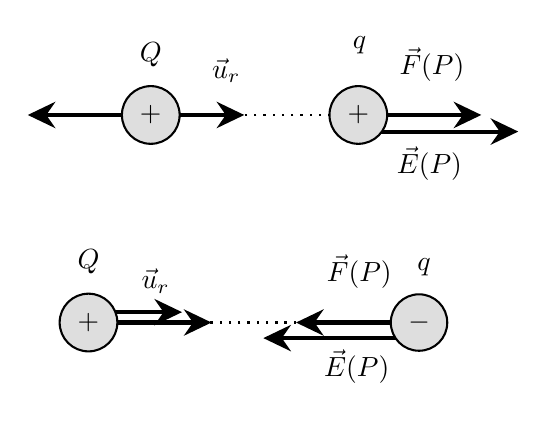
\begin{tikzpicture}[x=0.75pt,y=0.75pt,yscale=-1,xscale=1]
	%uncomment if require: \path (0,300); %set diagram left start at 0, and has height of 300

	%Straight Lines [id:da18862268387082737] 
	\draw [line width=1.5]    (174.75,50.75) -- (119.5,50.75) ;
	\draw [shift={(115.5,50.75)}, rotate = 360] [fill={rgb, 255:red, 0; green, 0; blue, 0 }  ][line width=0.08]  [draw opacity=0] (13.4,-6.43) -- (0,0) -- (13.4,6.44) -- (8.9,0) -- cycle    ;
	%Straight Lines [id:da608158656410348] 
	\draw [line width=1.5]    (330,50.75) -- (274.75,50.75) ;
	\draw [shift={(334,50.75)}, rotate = 180] [fill={rgb, 255:red, 0; green, 0; blue, 0 }  ][line width=0.08]  [draw opacity=0] (13.4,-6.43) -- (0,0) -- (13.4,6.44) -- (8.9,0) -- cycle    ;
	%Straight Lines [id:da8127149875512598] 
	\draw [line width=1.5]    (215.8,50.75) -- (174.75,50.75) ;
	\draw [shift={(219.8,50.75)}, rotate = 180] [fill={rgb, 255:red, 0; green, 0; blue, 0 }  ][line width=0.08]  [draw opacity=0] (13.4,-6.43) -- (0,0) -- (13.4,6.44) -- (8.9,0) -- cycle    ;
	%Straight Lines [id:da4900066534826375] 
	\draw [line width=0.75]  [dash pattern={on 0.84pt off 2.51pt}]  (274.75,50.75) -- (174.75,50.75) ;
	%Straight Lines [id:da43114939450056067] 
	\draw [line width=1.5]    (347.8,58.75) -- (274.75,58.75) ;
	\draw [shift={(351.8,58.75)}, rotate = 180] [fill={rgb, 255:red, 0; green, 0; blue, 0 }  ][line width=0.08]  [draw opacity=0] (13.4,-6.43) -- (0,0) -- (13.4,6.44) -- (8.9,0) -- cycle    ;
	%Straight Lines [id:da17578940519252795] 
	\draw [line width=1.5]    (304,150.75) -- (248.75,150.75) ;
	\draw [shift={(244.75,150.75)}, rotate = 360] [fill={rgb, 255:red, 0; green, 0; blue, 0 }  ][line width=0.08]  [draw opacity=0] (13.4,-6.43) -- (0,0) -- (13.4,6.44) -- (8.9,0) -- cycle    ;
	%Straight Lines [id:da8949433624753187] 
	\draw [line width=1.5]    (200,150.75) -- (144.75,150.75) ;
	\draw [shift={(204,150.75)}, rotate = 180] [fill={rgb, 255:red, 0; green, 0; blue, 0 }  ][line width=0.08]  [draw opacity=0] (13.4,-6.43) -- (0,0) -- (13.4,6.44) -- (8.9,0) -- cycle    ;
	%Straight Lines [id:da8755641170993631] 
	\draw [line width=1.5]    (185.8,145.75) -- (144.75,145.75) ;
	\draw [shift={(189.8,145.75)}, rotate = 180] [fill={rgb, 255:red, 0; green, 0; blue, 0 }  ][line width=0.08]  [draw opacity=0] (13.4,-6.43) -- (0,0) -- (13.4,6.44) -- (8.9,0) -- cycle    ;
	%Straight Lines [id:da2517549122221281] 
	\draw [line width=0.75]  [dash pattern={on 0.84pt off 2.51pt}]  (244.75,150.75) -- (144.75,150.75) ;
	%Straight Lines [id:da7204302662170563] 
	\draw [line width=1.5]    (233,158.25) -- (301.75,158.25) ;
	\draw [shift={(229,158.25)}, rotate = 0] [fill={rgb, 255:red, 0; green, 0; blue, 0 }  ][line width=0.08]  [draw opacity=0] (13.4,-6.43) -- (0,0) -- (13.4,6.44) -- (8.9,0) -- cycle    ;

	% Text Node
	\draw (174.8,21.5) node    {$Q$};
	% Text Node
	\draw (275.4,17.3) node    {$q$};
	% Text Node
	\draw (310.2,26.4) node    {$\vec{F}( P)$};
	% Text Node
	\draw (211.1,29.3) node    {$\vec{u}_{r}$};
	% Text Node
	\draw  [fill={rgb, 255:red, 222; green, 222; blue, 222 }  ,fill opacity=1 ]  (174.75, 50.75) circle [x radius= 13.9, y radius= 13.9]   ;
	\draw (174.75,50.75) node    {$+$};
	% Text Node
	\draw  [fill={rgb, 255:red, 222; green, 222; blue, 222 }  ,fill opacity=1 ]  (274.75, 50.75) circle [x radius= 13.9, y radius= 13.9]   ;
	\draw (274.75,50.75) node    {$+$};
	% Text Node
	\draw (309,74) node    {$\vec{E}( P)$};
	% Text Node
	\draw (144.8,121.5) node    {$Q$};
	% Text Node
	\draw (306.4,124.3) node    {$q$};
	% Text Node
	\draw (275.2,126.4) node    {$\vec{F}( P)$};
	% Text Node
	\draw (177.1,130.8) node    {$\vec{u}_{r}$};
	% Text Node
	\draw  [fill={rgb, 255:red, 222; green, 222; blue, 222 }  ,fill opacity=1 ]  (144.75, 150.75) circle [x radius= 13.9, y radius= 13.9]   ;
	\draw (144.75,150.75) node    {$+$};
	% Text Node
	\draw  [fill={rgb, 255:red, 222; green, 222; blue, 222 }  ,fill opacity=1 ]  (304, 150.75) circle [x radius= 13.6, y radius= 13.6]   ;
	\draw (304,150.75) node    {$-$};
	% Text Node
	\draw (274,172) node    {$\vec{E}( P)$};

	\end{tikzpicture}
\end{figure}
\FloatBarrier

In base alla definizione di campo elettrico, se lo abbiamo già calcolato, la forza agente sulla carica $q$ sarà semplicemente:

\[
	\vec{F} (P) = q\vec{E} (P)
\]

Quando consideriamo distribuzioni di carica molto complesse sarà un approccio preferibile.
Il campo elettrico in se non è misurabile direttamente, quello che possiamo fare è misurare la forza che la sorgente esercita sulla carica esploratrice.
La procedura di misura del campo elettrico può alterare il risultato che voglio ottenere perché se avvicino la carica esploratrice alla sorgente, quest'ultima si allontana a sua volta. In realtà il modo migliore di definire questo campo elettrico è di scegliere una carica esploratrice piccolissima, di modo che la sua influenza sulla sorgente sia minimale. Quindi una definizione più rigorosa di campo elettrico è la seguente:

\[
	\vec{E} (P)=\lim_{q \to 0}\frac{\vec{F} (P)}{q}
\]

Dove il limite è da intendersi non in senso analitico, ma in senso fisico, cioé prendere $q$ più piccola possibile.

Immaginiamo di avere un insieme di tante cariche e di voler determinare il valore del campo elettrico complessivo che la carica sorgente genera nello spazio. Per fare questo studiamo la risultante $\vec{R}$ delle forze che le varie cariche esercitano sulla esploratrice.

\[
	\vec{E} (P) = \frac{\vec{R} (P)}{q} = \frac{ \frac{\sum_i Q_i q \vec{u}_{r_i}}{4\pi \varepsilon_0 r_i^2}}{q} =  \frac{\sum_i Q_i \vec{u}_{r_i}}{4\pi \varepsilon_0 r_i^2}
\]

Il campo elettrico complessivo prodotto da questa distribuzione è semplicemente la somma dei campi elettrici che ciascuna carica produce. In questo senso il principio di sovrapposizione vale anche per i singoli campi elettrici. $\vec{u}_r$ si può scrivere anche come il vettore $\vec{r}_i$ diviso il suo modulo.

\[
	\vec{u}_{r_i} = \frac{\vec{r}_i}{r_i}
\]

Con tal scrittura il campo elettrico nel punto $P$ sarà:

\[
	\vec{E} (P) = \sum_i \frac{Q\vec{r}_i}{4\pi \varepsilon_0 r_i^3}
\]

\subsection{Rappresentazione cartesiana del campo elettrico}

Ci sono alcuni casi in cui il versore $\vec{u}_r$ e di conseguenza la distanza fra le cariche sono più complicati da calcolare. In questi casi ci si può anche cimentare su un calcolo basato sulla scomposizione cartesiana.
Vedendo le cose in questo modo potremmo anche pensare di introdurre i versori $\vec{u}_x$, $\vec{u}_y$, $\vec{u}_z$ e individuare la posizione della carica $Q$ e del punto $P$ con opportuni vettori come in figura.

\begin{figure}[htpb]
	\centering

	\tikzset{every picture/.style={line width=0.75pt}} %set default line width to 0.75pt        

	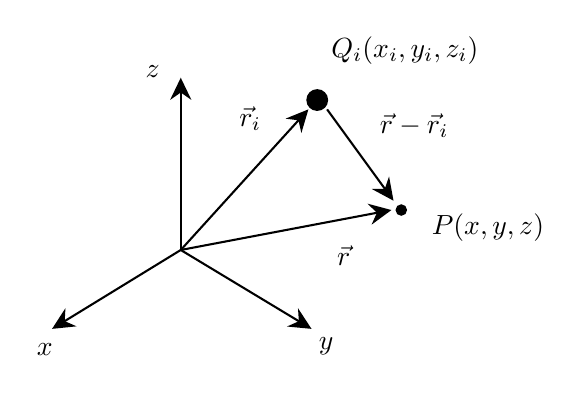
\begin{tikzpicture}[x=0.75pt,y=0.75pt,yscale=-1,xscale=1]
	%uncomment if require: \path (0,300); %set diagram left start at 0, and has height of 300

	%Straight Lines [id:da3359763454506417] 
	\draw    (199.5,160) -- (199.5,80) ;
	\draw [shift={(199.5,77)}, rotate = 450] [fill={rgb, 255:red, 0; green, 0; blue, 0 }  ][line width=0.08]  [draw opacity=0] (10.72,-5.15) -- (0,0) -- (10.72,5.15) -- (7.12,0) -- cycle    ;
	%Straight Lines [id:da41620874068539027] 
	\draw    (199.5,160) -- (259.93,196.45) ;
	\draw [shift={(262.5,198)}, rotate = 211.1] [fill={rgb, 255:red, 0; green, 0; blue, 0 }  ][line width=0.08]  [draw opacity=0] (10.72,-5.15) -- (0,0) -- (10.72,5.15) -- (7.12,0) -- cycle    ;
	%Straight Lines [id:da45968237944825696] 
	\draw    (199.5,160) -- (140.06,196.43) ;
	\draw [shift={(137.5,198)}, rotate = 328.5] [fill={rgb, 255:red, 0; green, 0; blue, 0 }  ][line width=0.08]  [draw opacity=0] (10.72,-5.15) -- (0,0) -- (10.72,5.15) -- (7.12,0) -- cycle    ;
	%Shape: Circle [id:dp9255160036546715] 
	\draw  [fill={rgb, 255:red, 0; green, 0; blue, 0 }  ,fill opacity=1 ] (260.5,87.75) .. controls (260.5,85.13) and (262.63,83) .. (265.25,83) .. controls (267.87,83) and (270,85.13) .. (270,87.75) .. controls (270,90.37) and (267.87,92.5) .. (265.25,92.5) .. controls (262.63,92.5) and (260.5,90.37) .. (260.5,87.75) -- cycle ;
	%Shape: Circle [id:dp6015853897023355] 
	\draw  [fill={rgb, 255:red, 0; green, 0; blue, 0 }  ,fill opacity=1 ] (303.5,140.75) .. controls (303.5,139.51) and (304.51,138.5) .. (305.75,138.5) .. controls (306.99,138.5) and (308,139.51) .. (308,140.75) .. controls (308,141.99) and (306.99,143) .. (305.75,143) .. controls (304.51,143) and (303.5,141.99) .. (303.5,140.75) -- cycle ;
	%Straight Lines [id:da3732851936378614] 
	\draw    (199.5,160) -- (258.98,94.47) ;
	\draw [shift={(261,92.25)}, rotate = 492.23] [fill={rgb, 255:red, 0; green, 0; blue, 0 }  ][line width=0.08]  [draw opacity=0] (10.72,-5.15) -- (0,0) -- (10.72,5.15) -- (7.12,0) -- cycle    ;
	%Straight Lines [id:da4541507595227321] 
	\draw    (199.5,160) -- (298.05,141.31) ;
	\draw [shift={(301,140.75)}, rotate = 529.26] [fill={rgb, 255:red, 0; green, 0; blue, 0 }  ][line width=0.08]  [draw opacity=0] (10.72,-5.15) -- (0,0) -- (10.72,5.15) -- (7.12,0) -- cycle    ;
	%Straight Lines [id:da09502568264571676] 
	\draw    (270,92.25) -- (300.24,133.82) ;
	\draw [shift={(302,136.25)}, rotate = 233.97] [fill={rgb, 255:red, 0; green, 0; blue, 0 }  ][line width=0.08]  [draw opacity=0] (10.72,-5.15) -- (0,0) -- (10.72,5.15) -- (7.12,0) -- cycle    ;

	% Text Node
	\draw (134,208) node    {$x$};
	% Text Node
	\draw (269.5,206.5) node    {$y$};
	% Text Node
	\draw (186,74) node    {$z$};
	% Text Node
	\draw (312,100) node    {$\vec{r} -\vec{r}_{i}$};
	% Text Node
	\draw (278,162.5) node    {$\vec{r}$};
	% Text Node
	\draw (233,96.5) node    {$\vec{r}_{i}$};
	% Text Node
	\draw (307.5,64) node    {$Q_{i}( x_{i} ,y_{i} ,z_{i})$};
	% Text Node
	\draw (347.5,149) node    {$P( x ,y,z)$};

	\end{tikzpicture}
\end{figure}
\FloatBarrier

Sia $Q_i(x_i,y_i,z_i)$ una generica carica al variare di $i$ e $P(x,y,z)$ un punto nello spazio. Consideriamo la distanza, vettoriale, fra questi due punti espressa da

\[
	\vec{r} - \vec{r}_i = (x-x_i )\vec{u}_x + (y-y_i )\vec{u}_y + (z-z_i)\vec{u}_z
\]

Allora il campo elettrico elettrico generato dalle cariche $Q_i$ sul punto $P$ vale

\begin{align*}
	\vec{E} (P) = E(x,y,z) &= \sum_i \frac{Q_i(\vec{r} - \vec{r}_i)}{4\pi \varepsilon_0 |\vec{r} -\vec{r}_i |^3} \\
	&= \sum_i \frac{Q_i [(x-x_i )\vec{u}_x + (y-y_i )\vec{u}_y + (z-z_i)\vec{u}_z]}{4\pi \varepsilon_0 [(x-x_i)^2 + (y-y_i)^2 + (z-z_i)^2]^{\frac{3}{2}}}
\end{align*}

A questo punto supponiamo di voler calcolare il campo elettrico generato da un oggetto in cui siamo riusciti a inserire un numero elevatissimo di cariche. Invece di vedere queste cariche come tantissime cariche puntiformi, possiamo fare l'ipotesi che la carica sia distribuita all'intero dell'oggetto con una certa continuità. Cercheremo di rappresentare cariche all'interno dell'oggetto con delle funzioni di distribuzione.

\begin{itemize}
	\item \emph{Densità di carica di volume} $\rho (x',y',z')$ \\
	Consideriamo ora un cubetto di volume $d\tau$ e carica $dq$ centrato in $P'(x',y',z')$. Sia $\vec{r}'$ variabile e $\vec{r}$ costante. Esprimiamo la carica $ dq = \rho (x',y',z') d\tau$ e il campo elettrico infinitesimo $ d\vec{E} = \frac{dq (\vec{r} -\vec{r}_i )}{4\pi \varepsilon_0 |\vec{r} -\vec{r}_i |^3} $ generato dalla distribuzione di carica nel punto $P$. Allora
	\begin{align*}
		\vec{E} (P) = \int_{\text{oggetto}} d\vec{E} &= \int_{\text{ogg.}} \frac{dq (\vec{r} -\vec{r}_i )}{4\pi \varepsilon_0 |\vec{r} -\vec{r}_i |^3}\\
		\vec{E} (P) &= \int_{\tau} \frac{\rho (x',y',z') d\tau (\vec{r} -\vec{r}_i )}{4\pi \varepsilon_0 |\vec{r} -\vec{r}_i |^3} \\
		\vec{E} (P) &= \int_{\tau} \frac{\rho (x',y',z') (\vec{r} -\vec{r}_i )}{4\pi \varepsilon_0 |\vec{r} -\vec{r}_i |^3}d\tau
	\end{align*}
	\begin{figure}[htpb]
		\centering
		

		\tikzset{every picture/.style={line width=0.75pt}} %set default line width to 0.75pt        

		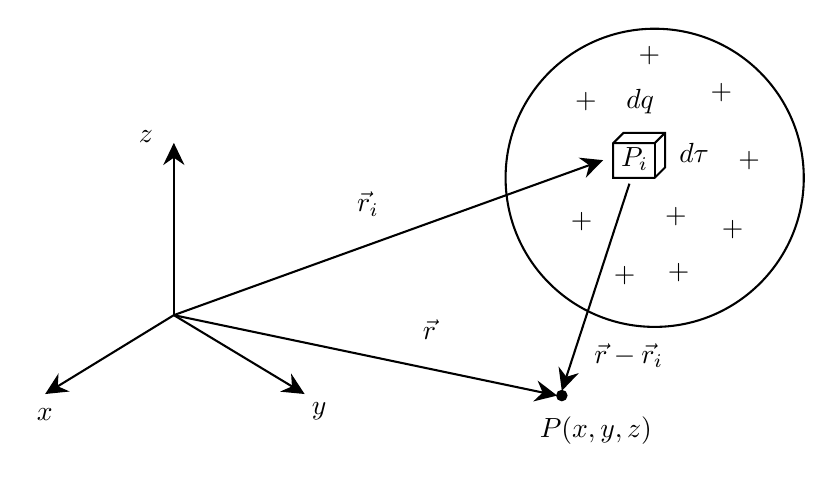
\begin{tikzpicture}[x=0.75pt,y=0.75pt,yscale=-1,xscale=1]
		%uncomment if require: \path (0,300); %set diagram left start at 0, and has height of 300

		%Straight Lines [id:da8420671197768959] 
		\draw    (217.5,208.67) -- (217.5,128.67) ;
		\draw [shift={(217.5,125.67)}, rotate = 450] [fill={rgb, 255:red, 0; green, 0; blue, 0 }  ][line width=0.08]  [draw opacity=0] (10.72,-5.15) -- (0,0) -- (10.72,5.15) -- (7.12,0) -- cycle    ;
		%Straight Lines [id:da5234979003637599] 
		\draw    (217.5,208.67) -- (277.93,245.12) ;
		\draw [shift={(280.5,246.67)}, rotate = 211.1] [fill={rgb, 255:red, 0; green, 0; blue, 0 }  ][line width=0.08]  [draw opacity=0] (10.72,-5.15) -- (0,0) -- (10.72,5.15) -- (7.12,0) -- cycle    ;
		%Straight Lines [id:da5970517142159921] 
		\draw    (217.5,208.67) -- (158.06,245.1) ;
		\draw [shift={(155.5,246.67)}, rotate = 328.5] [fill={rgb, 255:red, 0; green, 0; blue, 0 }  ][line width=0.08]  [draw opacity=0] (10.72,-5.15) -- (0,0) -- (10.72,5.15) -- (7.12,0) -- cycle    ;
		%Shape: Circle [id:dp8904353238466189] 
		\draw  [fill={rgb, 255:red, 0; green, 0; blue, 0 }  ,fill opacity=1 ] (402.17,247.42) .. controls (402.17,246.17) and (403.17,245.17) .. (404.42,245.17) .. controls (405.66,245.17) and (406.67,246.17) .. (406.67,247.42) .. controls (406.67,248.66) and (405.66,249.67) .. (404.42,249.67) .. controls (403.17,249.67) and (402.17,248.66) .. (402.17,247.42) -- cycle ;
		%Straight Lines [id:da20882025926140635] 
		\draw    (217.5,208.67) -- (421.51,135.02) ;
		\draw [shift={(424.33,134)}, rotate = 520.15] [fill={rgb, 255:red, 0; green, 0; blue, 0 }  ][line width=0.08]  [draw opacity=0] (10.72,-5.15) -- (0,0) -- (10.72,5.15) -- (7.12,0) -- cycle    ;
		%Straight Lines [id:da8503611158657807] 
		\draw    (217.5,208.67) -- (399.23,246.8) ;
		\draw [shift={(402.17,247.42)}, rotate = 191.85] [fill={rgb, 255:red, 0; green, 0; blue, 0 }  ][line width=0.08]  [draw opacity=0] (10.72,-5.15) -- (0,0) -- (10.72,5.15) -- (7.12,0) -- cycle    ;
		%Straight Lines [id:da9131411337431448] 
		\draw    (437,145.33) -- (405.35,242.31) ;
		\draw [shift={(404.42,245.17)}, rotate = 288.08] [fill={rgb, 255:red, 0; green, 0; blue, 0 }  ][line width=0.08]  [draw opacity=0] (10.72,-5.15) -- (0,0) -- (10.72,5.15) -- (7.12,0) -- cycle    ;
		%Shape: Circle [id:dp1522505573812425] 
		\draw   (377.33,142.5) .. controls (377.33,102.83) and (409.49,70.67) .. (449.17,70.67) .. controls (488.84,70.67) and (521,102.83) .. (521,142.5) .. controls (521,182.17) and (488.84,214.33) .. (449.17,214.33) .. controls (409.49,214.33) and (377.33,182.17) .. (377.33,142.5) -- cycle ;
		%Shape: Cube [id:dp20550893096799427] 
		\draw   (429.17,125.83) -- (434.17,120.83) -- (454.17,120.83) -- (454.17,137.5) -- (449.17,142.5) -- (429.17,142.5) -- cycle ; \draw   (454.17,120.83) -- (449.17,125.83) -- (429.17,125.83) ; \draw   (449.17,125.83) -- (449.17,142.5) ;

		% Text Node
		\draw (155.33,256.67) node    {$x$};
		% Text Node
		\draw (287.5,255.17) node    {$y$};
		% Text Node
		\draw (204,122.67) node    {$z$};
		% Text Node
		\draw (436.67,228) node    {$\vec{r} -\vec{r}_{i}$};
		% Text Node
		\draw (340.67,215.83) node    {$\vec{r}$};
		% Text Node
		\draw (311,155.17) node    {$\vec{r}_{i}$};
		% Text Node
		\draw (442.17,106) node    {$dq$};
		% Text Node
		\draw (420.83,264.33) node    {$P( x ,y,z)$};
		% Text Node
		\draw (446.67,83.67) node    {$+$};
		% Text Node
		\draw (481.33,101.67) node    {$+$};
		% Text Node
		\draw (494.67,134.33) node    {$+$};
		% Text Node
		\draw (486.67,167.67) node    {$+$};
		% Text Node
		\draw (460.67,188.33) node    {$+$};
		% Text Node
		\draw (434.67,189.67) node    {$+$};
		% Text Node
		\draw (414,163.67) node    {$+$};
		% Text Node
		\draw (416,105.67) node    {$+$};
		% Text Node
		\draw (459.33,161) node    {$+$};
		% Text Node
		\draw (439.5,133.33) node    {$P_{i}$};
		% Text Node
		\draw (468.17,130.67) node    {$d\tau $};

		\end{tikzpicture}
	\end{figure}
	\FloatBarrier

	\item \emph{Densità di carica superficiale} $\sigma (x',y',z') $ \\
	Consideriamo ora una superficie infinitesima $dS$ e carica $dq$ in $P'(x',y',z')$. Sia $\vec{r}'$ variabile e $\vec{r}$ costante. Esprimiamo la carica $dq=\sigma(x',y',z') dS$ e il campo elettrico infinitesimo $ d\vec{E} = \frac{dq (\vec{r} -\vec{r}_i )}{4\pi \varepsilon_0 |\vec{r} -\vec{r}_i |^3} $ generato dalla distribuzione di carica nel punto $P$. Allora
	\begin{align*}
		\vec{E} (P) &= \int_{\Sigma} \frac{\sigma  (x',y',z') (\vec{r} -\vec{r}_i )}{4\pi \varepsilon_0 |\vec{r} -\vec{r}_i |^3}dS
	\end{align*}
	\begin{figure}[htpb]
		\centering
		

		\tikzset{every picture/.style={line width=0.75pt}} %set default line width to 0.75pt        

		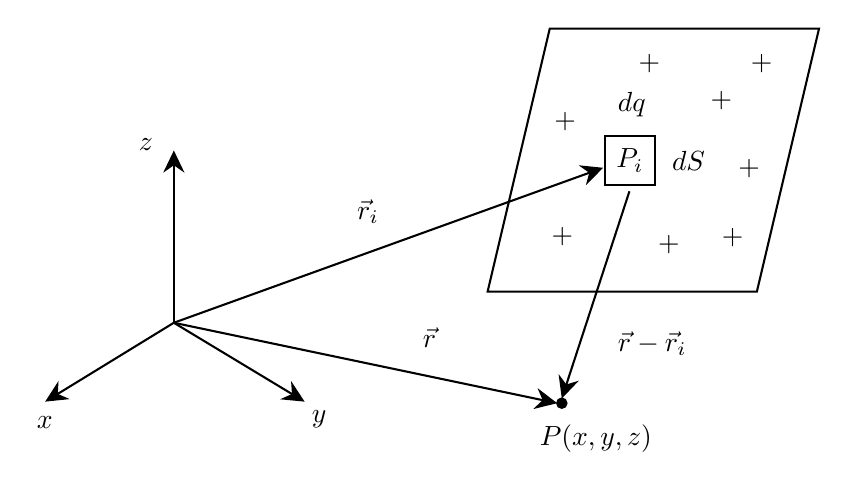
\begin{tikzpicture}[x=0.75pt,y=0.75pt,yscale=-1,xscale=1]
		%uncomment if require: \path (0,300); %set diagram left start at 0, and has height of 300

		%Straight Lines [id:da06313925185671954] 
		\draw    (177.5,189.67) -- (177.5,109.67) ;
		\draw [shift={(177.5,106.67)}, rotate = 450] [fill={rgb, 255:red, 0; green, 0; blue, 0 }  ][line width=0.08]  [draw opacity=0] (10.72,-5.15) -- (0,0) -- (10.72,5.15) -- (7.12,0) -- cycle    ;
		%Straight Lines [id:da7777160466511888] 
		\draw    (177.5,189.67) -- (237.93,226.12) ;
		\draw [shift={(240.5,227.67)}, rotate = 211.1] [fill={rgb, 255:red, 0; green, 0; blue, 0 }  ][line width=0.08]  [draw opacity=0] (10.72,-5.15) -- (0,0) -- (10.72,5.15) -- (7.12,0) -- cycle    ;
		%Straight Lines [id:da5510445060802585] 
		\draw    (177.5,189.67) -- (118.06,226.1) ;
		\draw [shift={(115.5,227.67)}, rotate = 328.5] [fill={rgb, 255:red, 0; green, 0; blue, 0 }  ][line width=0.08]  [draw opacity=0] (10.72,-5.15) -- (0,0) -- (10.72,5.15) -- (7.12,0) -- cycle    ;
		%Shape: Circle [id:dp5550712782342335] 
		\draw  [fill={rgb, 255:red, 0; green, 0; blue, 0 }  ,fill opacity=1 ] (362.17,228.42) .. controls (362.17,227.17) and (363.17,226.17) .. (364.42,226.17) .. controls (365.66,226.17) and (366.67,227.17) .. (366.67,228.42) .. controls (366.67,229.66) and (365.66,230.67) .. (364.42,230.67) .. controls (363.17,230.67) and (362.17,229.66) .. (362.17,228.42) -- cycle ;
		%Straight Lines [id:da39423175034912705] 
		\draw    (177.5,189.67) -- (381.51,116.02) ;
		\draw [shift={(384.33,115)}, rotate = 520.15] [fill={rgb, 255:red, 0; green, 0; blue, 0 }  ][line width=0.08]  [draw opacity=0] (10.72,-5.15) -- (0,0) -- (10.72,5.15) -- (7.12,0) -- cycle    ;
		%Straight Lines [id:da7865572141870176] 
		\draw    (177.5,189.67) -- (359.23,227.8) ;
		\draw [shift={(362.17,228.42)}, rotate = 191.85] [fill={rgb, 255:red, 0; green, 0; blue, 0 }  ][line width=0.08]  [draw opacity=0] (10.72,-5.15) -- (0,0) -- (10.72,5.15) -- (7.12,0) -- cycle    ;
		%Straight Lines [id:da8495210953077466] 
		\draw    (397,126.33) -- (365.35,223.31) ;
		\draw [shift={(364.42,226.17)}, rotate = 288.08] [fill={rgb, 255:red, 0; green, 0; blue, 0 }  ][line width=0.08]  [draw opacity=0] (10.72,-5.15) -- (0,0) -- (10.72,5.15) -- (7.12,0) -- cycle    ;
		%Flowchart: Data [id:dp2491781918344611] 
		\draw   (358.6,48) -- (488.33,48) -- (458.4,174.67) -- (328.67,174.67) -- cycle ;
		%Shape: Square [id:dp7066276931584026] 
		\draw   (385.17,99.5) -- (409.17,99.5) -- (409.17,123.5) -- (385.17,123.5) -- cycle ;

		% Text Node
		\draw (115.33,237.67) node    {$x$};
		% Text Node
		\draw (247.5,236.17) node    {$y$};
		% Text Node
		\draw (164,103.67) node    {$z$};
		% Text Node
		\draw (408,199.67) node    {$\vec{r} -\vec{r}_{i}$};
		% Text Node
		\draw (300.67,196.83) node    {$\vec{r}$};
		% Text Node
		\draw (271,136.17) node    {$\vec{r}_{i}$};
		% Text Node
		\draw (398.17,84.33) node    {$dq$};
		% Text Node
		\draw (380.83,245.33) node    {$P( x ,y,z)$};
		% Text Node
		\draw (406.67,64.67) node    {$+$};
		% Text Node
		\draw (441.33,82.67) node    {$+$};
		% Text Node
		\draw (454.67,115.33) node    {$+$};
		% Text Node
		\draw (446.67,148.67) node    {$+$};
		% Text Node
		\draw (460.67,64.67) node    {$+$};
		% Text Node
		\draw (364.67,148) node    {$+$};
		% Text Node
		\draw (366,92.67) node    {$+$};
		% Text Node
		\draw (416,152) node    {$+$};
		% Text Node
		\draw (397.17,111.5) node    {$P_{i}$};
		% Text Node
		\draw (425.5,111.67) node    {$dS$};

		\end{tikzpicture}
	\end{figure}
	\FloatBarrier

	\item \emph{Densità di carica lineare} $\lambda (x',y',z') $ \\
	Consideriamo ora un segmento infinitesimo $dl$ e carica $dq$ in $P'(x',y',z')$. Sia $\vec{r}'$ variabile e $\vec{r}$ costante. Esprimiamo la carica $ dq = \lambda(x',y',z') dl $ e il campo elettrico infinitesimo $d\vec{E} = \frac{dq (\vec{r} -\vec{r}_i )}{4\pi \varepsilon_0 |\vec{r} -\vec{r}_i |^3}$ generato dalla distribuzione di carica nel punto $P$. Allora
	\begin{align*}
		\vec{E} (P) &= \int_{\Lambda} \frac{\lambda  (x',y',z') (\vec{r} -\vec{r}_i )}{4\pi \varepsilon_0 |\vec{r} -\vec{r}_i |^3}dl
	\end{align*}
	\begin{figure}[htpb]
		\centering
		

		\tikzset{every picture/.style={line width=0.75pt}} %set default line width to 0.75pt        

		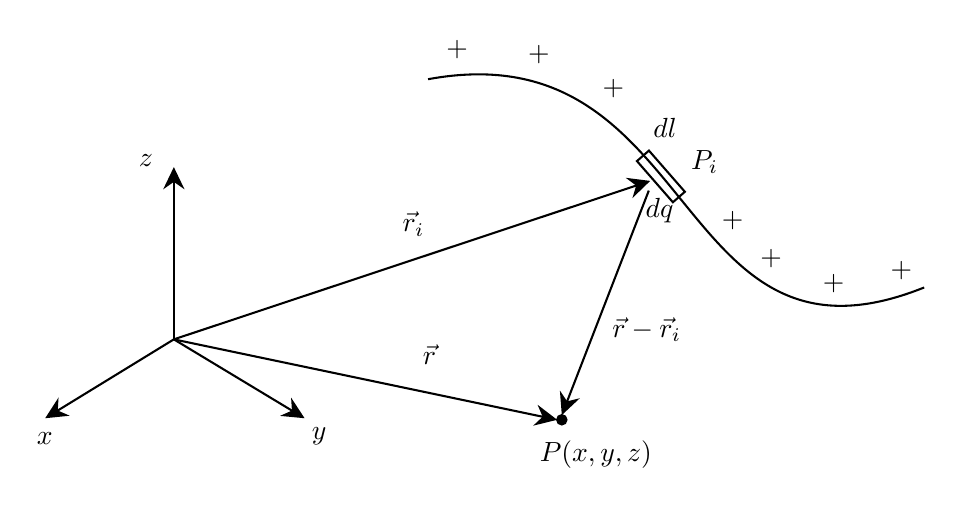
\begin{tikzpicture}[x=0.75pt,y=0.75pt,yscale=-1,xscale=1]
		%uncomment if require: \path (0,300); %set diagram left start at 0, and has height of 300

		%Straight Lines [id:da2742946758986795] 
		\draw    (197.5,209.67) -- (197.5,129.67) ;
		\draw [shift={(197.5,126.67)}, rotate = 450] [fill={rgb, 255:red, 0; green, 0; blue, 0 }  ][line width=0.08]  [draw opacity=0] (10.72,-5.15) -- (0,0) -- (10.72,5.15) -- (7.12,0) -- cycle    ;
		%Straight Lines [id:da1582112085793861] 
		\draw    (197.5,209.67) -- (257.93,246.12) ;
		\draw [shift={(260.5,247.67)}, rotate = 211.1] [fill={rgb, 255:red, 0; green, 0; blue, 0 }  ][line width=0.08]  [draw opacity=0] (10.72,-5.15) -- (0,0) -- (10.72,5.15) -- (7.12,0) -- cycle    ;
		%Straight Lines [id:da5400686138190309] 
		\draw    (197.5,209.67) -- (138.06,246.1) ;
		\draw [shift={(135.5,247.67)}, rotate = 328.5] [fill={rgb, 255:red, 0; green, 0; blue, 0 }  ][line width=0.08]  [draw opacity=0] (10.72,-5.15) -- (0,0) -- (10.72,5.15) -- (7.12,0) -- cycle    ;
		%Shape: Circle [id:dp6260213863639099] 
		\draw  [fill={rgb, 255:red, 0; green, 0; blue, 0 }  ,fill opacity=1 ] (382.17,248.42) .. controls (382.17,247.17) and (383.17,246.17) .. (384.42,246.17) .. controls (385.66,246.17) and (386.67,247.17) .. (386.67,248.42) .. controls (386.67,249.66) and (385.66,250.67) .. (384.42,250.67) .. controls (383.17,250.67) and (382.17,249.66) .. (382.17,248.42) -- cycle ;
		%Straight Lines [id:da4980329673200876] 
		\draw    (197.5,209.67) -- (424.15,134.28) ;
		\draw [shift={(427,133.33)}, rotate = 521.6] [fill={rgb, 255:red, 0; green, 0; blue, 0 }  ][line width=0.08]  [draw opacity=0] (10.72,-5.15) -- (0,0) -- (10.72,5.15) -- (7.12,0) -- cycle    ;
		%Straight Lines [id:da318682975442671] 
		\draw    (197.5,209.67) -- (379.23,247.8) ;
		\draw [shift={(382.17,248.42)}, rotate = 191.85] [fill={rgb, 255:red, 0; green, 0; blue, 0 }  ][line width=0.08]  [draw opacity=0] (10.72,-5.15) -- (0,0) -- (10.72,5.15) -- (7.12,0) -- cycle    ;
		%Straight Lines [id:da939671023931534] 
		\draw    (426.33,138) -- (385.5,243.37) ;
		\draw [shift={(384.42,246.17)}, rotate = 291.18] [fill={rgb, 255:red, 0; green, 0; blue, 0 }  ][line width=0.08]  [draw opacity=0] (10.72,-5.15) -- (0,0) -- (10.72,5.15) -- (7.12,0) -- cycle    ;
		%Curve Lines [id:da9500837709709089] 
		\draw    (320,84.33) .. controls (452.33,60) and (436.33,234) .. (559,184.67) ;
		%Shape: Rectangle [id:dp5919414273162227] 
		\draw   (426.4,118.73) -- (443.71,138.57) -- (437.94,143.61) -- (420.62,123.77) -- cycle ;

		% Text Node
		\draw (135.33,257.67) node    {$x$};
		% Text Node
		\draw (267.5,256.17) node    {$y$};
		% Text Node
		\draw (184,123.67) node    {$z$};
		% Text Node
		\draw (425.33,205) node    {$\vec{r} -\vec{r}_{i}$};
		% Text Node
		\draw (320.67,216.83) node    {$\vec{r}$};
		% Text Node
		\draw (313,154.17) node    {$\vec{r}_{i}$};
		% Text Node
		\draw (431.5,147.67) node    {$dq$};
		% Text Node
		\draw (400.83,265.33) node    {$P( x ,y,z)$};
		% Text Node
		\draw (334,70) node    {$+$};
		% Text Node
		\draw (409.33,88.67) node    {$+$};
		% Text Node
		\draw (485.33,170.67) node    {$+$};
		% Text Node
		\draw (515.33,182.67) node    {$+$};
		% Text Node
		\draw (373.33,72.67) node    {$+$};
		% Text Node
		\draw (548,176.67) node    {$+$};
		% Text Node
		\draw (453.17,124.17) node    {$P_{i}$};
		% Text Node
		\draw (434.17,107.67) node    {$dl$};
		% Text Node
		\draw (466.67,152.67) node    {$+$};

		\end{tikzpicture}
	\end{figure}
	\FloatBarrier

\end{itemize}

\section{Campo elettrico di un filo rettilineo infinito}

La dimostrazione suppone $\lambda$ costante.

\begin{figure}[htpb]
	\centering

	\tikzset{every picture/.style={line width=0.75pt}} %set default line width to 0.75pt        

	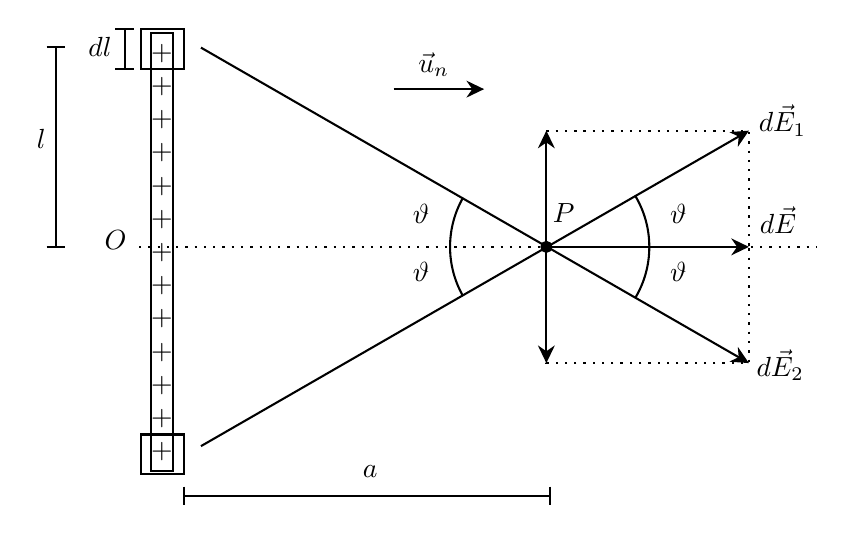
\begin{tikzpicture}[x=0.75pt,y=0.75pt,yscale=-0.8,xscale=0.8]
	%uncomment if require: \path (0,393); %set diagram left start at 0, and has height of 393

	%Shape: Rectangle [id:dp44310977854933165] 
	\draw   (140,81) -- (153,81) -- (153,345) -- (140,345) -- cycle ;
	%Straight Lines [id:da3097942485491145] 
	\draw  [dash pattern={on 0.84pt off 2.51pt}]  (132.67,210) -- (540.33,210) ;
	%Straight Lines [id:da7374934618400164] 
	\draw    (170,90) -- (497.4,278.5) ;
	\draw [shift={(500,280)}, rotate = 209.93] [fill={rgb, 255:red, 0; green, 0; blue, 0 }  ][line width=0.08]  [draw opacity=0] (10.72,-5.15) -- (0,0) -- (10.72,5.15) -- (7.12,0) -- cycle    ;
	%Straight Lines [id:da8123119214956673] 
	\draw    (170,330) -- (497.4,141.5) ;
	\draw [shift={(500,140)}, rotate = 510.07] [fill={rgb, 255:red, 0; green, 0; blue, 0 }  ][line width=0.08]  [draw opacity=0] (10.72,-5.15) -- (0,0) -- (10.72,5.15) -- (7.12,0) -- cycle    ;
	%Shape: Arc [id:dp1380381757942739] 
	\draw  [draw opacity=0] (327.56,239.18) .. controls (322.74,230.54) and (320,220.59) .. (320,210) .. controls (320,199.22) and (322.85,189.1) .. (327.83,180.35) -- (380,210) -- cycle ; \draw   (327.56,239.18) .. controls (322.74,230.54) and (320,220.59) .. (320,210) .. controls (320,199.22) and (322.85,189.1) .. (327.83,180.35) ;
	%Shape: Arc [id:dp4414106025648661] 
	\draw  [draw opacity=0] (431.46,179.14) .. controls (436.88,188.16) and (440,198.71) .. (440,210) .. controls (440,221.11) and (436.98,231.52) .. (431.71,240.45) -- (380,210) -- cycle ; \draw   (431.46,179.14) .. controls (436.88,188.16) and (440,198.71) .. (440,210) .. controls (440,221.11) and (436.98,231.52) .. (431.71,240.45) ;
	%Shape: Rectangle [id:dp8309920268613575] 
	\draw   (134,79) -- (160,79) -- (160,103) -- (134,103) -- cycle ;
	%Shape: Rectangle [id:dp19702818666456712] 
	\draw   (134,323) -- (160,323) -- (160,347) -- (134,347) -- cycle ;
	%Straight Lines [id:da37058240455784275] 
	\draw    (160,360) -- (380,360) ;
	\draw [shift={(380,360)}, rotate = 180] [color={rgb, 255:red, 0; green, 0; blue, 0 }  ][line width=0.75]    (0,5.59) -- (0,-5.59)   ;
	\draw [shift={(160,360)}, rotate = 180] [color={rgb, 255:red, 0; green, 0; blue, 0 }  ][line width=0.75]    (0,5.59) -- (0,-5.59)   ;
	%Shape: Circle [id:dp07344677800481558] 
	\draw  [fill={rgb, 255:red, 0; green, 0; blue, 0 }  ,fill opacity=1 ] (375,210) .. controls (375,208.34) and (376.34,207) .. (378,207) .. controls (379.66,207) and (381,208.34) .. (381,210) .. controls (381,211.66) and (379.66,213) .. (378,213) .. controls (376.34,213) and (375,211.66) .. (375,210) -- cycle ;
	%Straight Lines [id:da17272746827516716] 
	\draw    (82.67,210) -- (82.67,89.83) ;
	\draw [shift={(82.67,89.83)}, rotate = 450] [color={rgb, 255:red, 0; green, 0; blue, 0 }  ][line width=0.75]    (0,5.59) -- (0,-5.59)   ;
	\draw [shift={(82.67,210)}, rotate = 450] [color={rgb, 255:red, 0; green, 0; blue, 0 }  ][line width=0.75]    (0,5.59) -- (0,-5.59)   ;
	%Straight Lines [id:da06771818672423668] 
	\draw    (124,103) -- (124,79) ;
	\draw [shift={(124,79)}, rotate = 450] [color={rgb, 255:red, 0; green, 0; blue, 0 }  ][line width=0.75]    (0,5.59) -- (0,-5.59)   ;
	\draw [shift={(124,103)}, rotate = 450] [color={rgb, 255:red, 0; green, 0; blue, 0 }  ][line width=0.75]    (0,5.59) -- (0,-5.59)   ;
	%Shape: Rectangle [id:dp19188739834462787] 
	\draw  [dash pattern={on 0.84pt off 2.51pt}] (378,140) -- (500,140) -- (500,210) -- (378,210) -- cycle ;
	%Straight Lines [id:da2401580892794155] 
	\draw    (378,210) -- (378,143) ;
	\draw [shift={(378,140)}, rotate = 450] [fill={rgb, 255:red, 0; green, 0; blue, 0 }  ][line width=0.08]  [draw opacity=0] (10.72,-5.15) -- (0,0) -- (10.72,5.15) -- (7.12,0) -- cycle    ;
	%Straight Lines [id:da7211816669864399] 
	\draw    (378,210) -- (378,277) ;
	\draw [shift={(378,280)}, rotate = 270] [fill={rgb, 255:red, 0; green, 0; blue, 0 }  ][line width=0.08]  [draw opacity=0] (10.72,-5.15) -- (0,0) -- (10.72,5.15) -- (7.12,0) -- cycle    ;
	%Shape: Rectangle [id:dp6422672802074842] 
	\draw  [dash pattern={on 0.84pt off 2.51pt}] (378,210) -- (500,210) -- (500,280) -- (378,280) -- cycle ;
	%Straight Lines [id:da4577026773595012] 
	\draw    (378,210) -- (497,210) ;
	\draw [shift={(500,210)}, rotate = 180] [fill={rgb, 255:red, 0; green, 0; blue, 0 }  ][line width=0.08]  [draw opacity=0] (10.72,-5.15) -- (0,0) -- (10.72,5.15) -- (7.12,0) -- cycle    ;
	%Straight Lines [id:da21003998909834887] 
	\draw    (286,115) -- (337.5,115) ;
	\draw [shift={(340.5,115)}, rotate = 180] [fill={rgb, 255:red, 0; green, 0; blue, 0 }  ][line width=0.08]  [draw opacity=0] (10.72,-5.15) -- (0,0) -- (10.72,5.15) -- (7.12,0) -- cycle    ;

	% Text Node
	\draw (146.4,93.4) node    {$+$};
	% Text Node
	\draw (146.4,113.4) node    {$+$};
	% Text Node
	\draw (146.4,133.4) node    {$+$};
	% Text Node
	\draw (146.4,153.4) node    {$+$};
	% Text Node
	\draw (146.4,173.4) node    {$+$};
	% Text Node
	\draw (146.4,193.4) node    {$+$};
	% Text Node
	\draw (146.4,213.4) node    {$+$};
	% Text Node
	\draw (146.4,233.4) node    {$+$};
	% Text Node
	\draw (146.4,253.4) node    {$+$};
	% Text Node
	\draw (146.4,273.4) node    {$+$};
	% Text Node
	\draw (146.4,293.4) node    {$+$};
	% Text Node
	\draw (146.4,313.4) node    {$+$};
	% Text Node
	\draw (146.4,333.4) node    {$+$};
	% Text Node
	\draw (118.5,206) node    {$O$};
	% Text Node
	\draw (302.5,190) node    {$\vartheta $};
	% Text Node
	\draw (302.5,225) node    {$\vartheta $};
	% Text Node
	\draw (457.5,190) node    {$\vartheta $};
	% Text Node
	\draw (457.5,225) node    {$\vartheta $};
	% Text Node
	\draw (388.5,189.33) node    {$P$};
	% Text Node
	\draw (271.83,345.33) node    {$a$};
	% Text Node
	\draw (73.83,144.67) node    {$l$};
	% Text Node
	\draw (109.17,89.33) node    {$dl$};
	% Text Node
	\draw (520.17,134) node    {$d\vec{E}_{1}$};
	% Text Node
	\draw (518.83,281.33) node    {$d\vec{E}_{2}$};
	% Text Node
	\draw (517.5,194) node    {$d\vec{E}$};
	% Text Node
	\draw (310.17,100) node    {$\vec{u}_{n}$};

	\end{tikzpicture}
\end{figure}
\FloatBarrier

L'idea per fare questo tipo di dimostrazioni è ricordarsi quale sia l'angolo ``migliore'' da prendere come parametro, poi dare dei nomi appropriati a tutte le altre variabili e infine cercare una relazione tra le variabili e l'angolo, il quale infine andrà integrato.

\begin{gather*}
	|d\vec{E}_1|=\frac{dq}{4\pi \varepsilon_0 r^2}=\frac{\lambda dl}{4\pi \varepsilon_0 r^2} \\
	d\vec{E} = d\vec{E}_1+d\vec{E}_2 = 2|d\vec{E}_1 |\cos \vartheta \:\vec{u}_n = \frac{\lambda \, dl \, \cos \vartheta  \, \vec{u}_n}{2\pi \varepsilon_0 r^2}
\end{gather*}

Ora esplicitiamo gli altri termini in funzione dell'angolo $\vartheta$:

\begin{gather*}
	a=r\cos \vartheta  \; \implies  \; r=\frac{a}{\cos  \vartheta} \\
	\frac{l}{a}=\tan \vartheta \implies l=a \tan \vartheta  \implies dl=\frac{dl}{d\vartheta}d\vartheta =\frac{a}{\cos^2 \vartheta}d\vartheta
\end{gather*}

Sostituendo in $d\vec{E}$,

\begin{align*}
	d\vec{E} &= \frac{\lambda\vec{u}_n}{2\pi \varepsilon_0} \frac{ad\vartheta}{\cos^2 \vartheta} \frac{\cos \vartheta \vec{u}_n}{\left( \frac{a}{\cos \vartheta} \right)^2} = \frac{\lambda\cos \vartheta d\vartheta}{2\pi \varepsilon_0 a}\vec{u}_n \\
	\vec{E} &= \int_0^{\pi /2} d\vec{E} = \frac{\lambda \vec{u}_n}{2\pi \varepsilon_0 a} \underbrace{\int_0^{\pi /2} \cos \vartheta d\vartheta}_1 \tag*{integrando} \\
	\Aboxed{\vec{E} &= \frac{\lambda}{2\pi \varepsilon_0 a}\vec{u}_n}
\end{align*}

\section{Linee di forza del campo elettrostatico}

L'introduzione del concetto di campo elettrostatico mette in evidenza che la presenza di un sistema di cariche modifica lo spazio circostante, nel senso che una carica di prova posta in un qualsiasi punto risente della forza. Partendo da una generica posizione e muovendosi per tratti infinitesimi successivi, ciascuno parallelo e concorde al campo elettrostatico in quel dato punto, si ottiene una linea che è detta \textbf{linea di forza} o \textbf{linea di campo}. Essa è orientata e in ogni suo punto risulta tangente e di verso concorde al campo $\vec{v}(P)$ valutato nello stesso punto.

\begin{figure}[htpb]
	\centering

	\tikzset{every picture/.style={line width=0.75pt}} %set default line width to 0.75pt        

	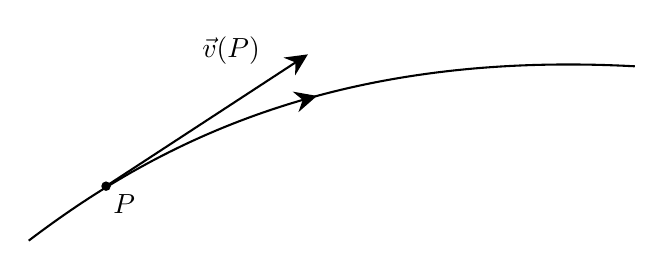
\begin{tikzpicture}[x=0.75pt,y=0.75pt,yscale=-1,xscale=1]
	%uncomment if require: \path (0,300); %set diagram left start at 0, and has height of 300

	%Curve Lines [id:da886214435685617] 
	\draw    (105.5,166) .. controls (163.5,122) and (249.5,74) .. (397.5,82) ;
	\draw [shift={(244.38,96.27)}, rotate = 524.4] [fill={rgb, 255:red, 0; green, 0; blue, 0 }  ][line width=0.08]  [draw opacity=0] (10.72,-5.15) -- (0,0) -- (10.72,5.15) -- (7.12,0) -- cycle    ;
	%Straight Lines [id:da4705565705020258] 
	\draw    (142.75,139.75) -- (237.49,77.89) ;
	\draw [shift={(240,76.25)}, rotate = 506.86] [fill={rgb, 255:red, 0; green, 0; blue, 0 }  ][line width=0.08]  [draw opacity=0] (10.72,-5.15) -- (0,0) -- (10.72,5.15) -- (7.12,0) -- cycle    ;
	%Shape: Circle [id:dp5625214438520421] 
	\draw  [fill={rgb, 255:red, 0; green, 0; blue, 0 }  ,fill opacity=1 ] (141,139.75) .. controls (141,138.78) and (141.78,138) .. (142.75,138) .. controls (143.72,138) and (144.5,138.78) .. (144.5,139.75) .. controls (144.5,140.72) and (143.72,141.5) .. (142.75,141.5) .. controls (141.78,141.5) and (141,140.72) .. (141,139.75) -- cycle ;

	% Text Node
	\draw (203,74.5) node    {$\vec{v}( P)$};
	% Text Node
	\draw (151.5,148.5) node    {$P$};

	\end{tikzpicture}
\end{figure}
\FloatBarrier

Se vogliamo rappresentare un campo vettoriale graficamente avremo un insieme di linee di flusso orientate che rappresentano l'andamento del campo.
Evidenziamo le proprietà principali delle linee di forza:

\begin{itemize}
	\item Per ogni punto $P$ in cui il campo $\vec{v}(P)$ definito è non nullo, passa una ed una sola linea di flusso (il campo in un punto è univocamente determinato).
	\item Nei casi particolari in cui più linee di flusso convergono verso un punto $P$, $P$ è sorgente negativa o pozzo delle linee di flusso.
	\item Nei casi particolari in cui più linee di flusso si diramano a partire da un punto $P$, diremo che quel punto è una sorgente positiva delle linee di flusso.
	\item Per campi vettoriali uniformi, in cui modulo direzione e verso sono costanti nello spazio, le linee di flusso sono linee rette parallele.
	\item Le linee di forza si addensano dove l'intensità del campo è maggiore.
	\item Una linea di forza in ogni suo punto è tangente e concorde al campo in quel punto.
	\item Le linee di forza hanno origine dalle cariche positive e terminano sulle cariche negative. Qualora ci siano solo cariche di uno stesso segno le linee di forza si chiudono all'infinito.
	\item Nel caso di cariche di segno opposto, ma eguali in modulo, tutte le linee che partono dalle cariche positive si chiudono sulle cariche negative, alcune passando eventualmente per l'infinito. Se invece le cariche non sono eguali in modulo, alcune linee terminano o provengono dall'infinito.
\end{itemize}

\begin{figure}[htpb]
	\centering

	\tikzset{every picture/.style={line width=0.75pt}} %set default line width to 0.75pt        

	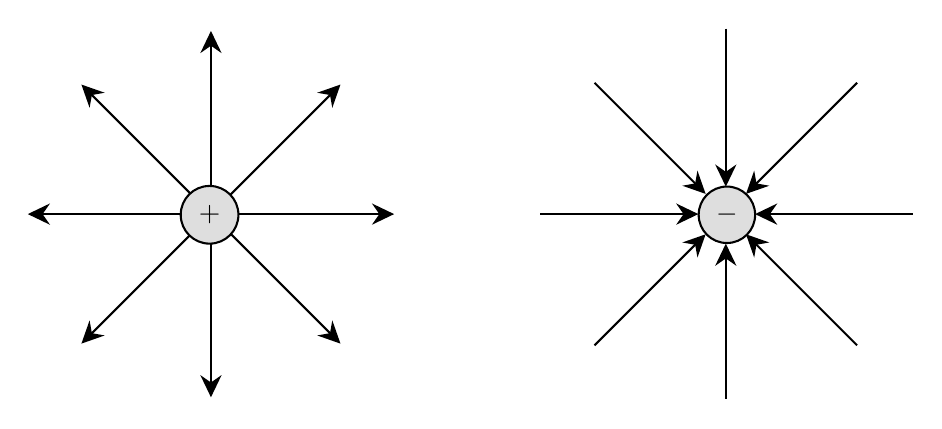
\begin{tikzpicture}[x=0.75pt,y=0.75pt,yscale=-1,xscale=1]
	%uncomment if require: \path (0,300); %set diagram left start at 0, and has height of 300

	%Straight Lines [id:da01701154185838294] 
	\draw    (175.42,150.42) -- (235.7,90.14) ;
	\draw [shift={(237.82,88.01)}, rotate = 495] [fill={rgb, 255:red, 0; green, 0; blue, 0 }  ][line width=0.08]  [draw opacity=0] (10.72,-5.15) -- (0,0) -- (10.72,5.15) -- (7.12,0) -- cycle    ;
	%Straight Lines [id:da12523204391835363] 
	\draw    (115.14,210.7) -- (175.42,150.42) ;
	\draw [shift={(113.01,212.82)}, rotate = 315] [fill={rgb, 255:red, 0; green, 0; blue, 0 }  ][line width=0.08]  [draw opacity=0] (10.72,-5.15) -- (0,0) -- (10.72,5.15) -- (7.12,0) -- cycle    ;
	%Straight Lines [id:da48631543354363305] 
	\draw    (175.42,150.42) -- (235.7,210.7) ;
	\draw [shift={(237.82,212.82)}, rotate = 225] [fill={rgb, 255:red, 0; green, 0; blue, 0 }  ][line width=0.08]  [draw opacity=0] (10.72,-5.15) -- (0,0) -- (10.72,5.15) -- (7.12,0) -- cycle    ;
	%Straight Lines [id:da7261478359039628] 
	\draw    (115.14,90.14) -- (175.42,150.42) ;
	\draw [shift={(113.01,88.01)}, rotate = 45] [fill={rgb, 255:red, 0; green, 0; blue, 0 }  ][line width=0.08]  [draw opacity=0] (10.72,-5.15) -- (0,0) -- (10.72,5.15) -- (7.12,0) -- cycle    ;
	%Straight Lines [id:da7554190837838399] 
	\draw    (175.42,150.42) -- (260.67,150.42) ;
	\draw [shift={(263.67,150.42)}, rotate = 180] [fill={rgb, 255:red, 0; green, 0; blue, 0 }  ][line width=0.08]  [draw opacity=0] (10.72,-5.15) -- (0,0) -- (10.72,5.15) -- (7.12,0) -- cycle    ;
	%Straight Lines [id:da014485419811356648] 
	\draw    (90.17,150.42) -- (175.42,150.42) ;
	\draw [shift={(87.17,150.42)}, rotate = 360] [fill={rgb, 255:red, 0; green, 0; blue, 0 }  ][line width=0.08]  [draw opacity=0] (10.72,-5.15) -- (0,0) -- (10.72,5.15) -- (7.12,0) -- cycle    ;
	%Straight Lines [id:da9699072893325926] 
	\draw    (175.42,150.42) -- (175.42,235.67) ;
	\draw [shift={(175.42,238.67)}, rotate = 270] [fill={rgb, 255:red, 0; green, 0; blue, 0 }  ][line width=0.08]  [draw opacity=0] (10.72,-5.15) -- (0,0) -- (10.72,5.15) -- (7.12,0) -- cycle    ;
	%Straight Lines [id:da5695531836183898] 
	\draw    (175.42,65.17) -- (175.42,150.42) ;
	\draw [shift={(175.42,62.17)}, rotate = 90] [fill={rgb, 255:red, 0; green, 0; blue, 0 }  ][line width=0.08]  [draw opacity=0] (10.72,-5.15) -- (0,0) -- (10.72,5.15) -- (7.12,0) -- cycle    ;
	%Straight Lines [id:da1847540335451905] 
	\draw    (435.34,138.56) -- (486.72,87.17) ;
	\draw [shift={(433.21,140.68)}, rotate = 315] [fill={rgb, 255:red, 0; green, 0; blue, 0 }  ][line width=0.08]  [draw opacity=0] (10.72,-5.15) -- (0,0) -- (10.72,5.15) -- (7.12,0) -- cycle    ;
	%Straight Lines [id:da5233688237452658] 
	\draw    (360.24,213.66) -- (411.62,162.27) ;
	\draw [shift={(413.75,160.15)}, rotate = 495] [fill={rgb, 255:red, 0; green, 0; blue, 0 }  ][line width=0.08]  [draw opacity=0] (10.72,-5.15) -- (0,0) -- (10.72,5.15) -- (7.12,0) -- cycle    ;
	%Straight Lines [id:da16846293285064373] 
	\draw    (435.34,162.27) -- (486.72,213.66) ;
	\draw [shift={(433.21,160.15)}, rotate = 45] [fill={rgb, 255:red, 0; green, 0; blue, 0 }  ][line width=0.08]  [draw opacity=0] (10.72,-5.15) -- (0,0) -- (10.72,5.15) -- (7.12,0) -- cycle    ;
	%Straight Lines [id:da05635078284520678] 
	\draw    (360.24,87.17) -- (411.62,138.56) ;
	\draw [shift={(413.75,140.68)}, rotate = 225] [fill={rgb, 255:red, 0; green, 0; blue, 0 }  ][line width=0.08]  [draw opacity=0] (10.72,-5.15) -- (0,0) -- (10.72,5.15) -- (7.12,0) -- cycle    ;
	%Straight Lines [id:da1612606104555494] 
	\draw    (440.58,150.42) -- (513.67,150.42) ;
	\draw [shift={(437.58,150.42)}, rotate = 0] [fill={rgb, 255:red, 0; green, 0; blue, 0 }  ][line width=0.08]  [draw opacity=0] (10.72,-5.15) -- (0,0) -- (10.72,5.15) -- (7.12,0) -- cycle    ;
	%Straight Lines [id:da4849446243609239] 
	\draw    (334.17,150.42) -- (407.25,150.42) ;
	\draw [shift={(410.25,150.42)}, rotate = 540] [fill={rgb, 255:red, 0; green, 0; blue, 0 }  ][line width=0.08]  [draw opacity=0] (10.72,-5.15) -- (0,0) -- (10.72,5.15) -- (7.12,0) -- cycle    ;
	%Straight Lines [id:da6572115408819028] 
	\draw    (423.48,167.65) -- (423.48,239.73) ;
	\draw [shift={(423.48,164.65)}, rotate = 90] [fill={rgb, 255:red, 0; green, 0; blue, 0 }  ][line width=0.08]  [draw opacity=0] (10.72,-5.15) -- (0,0) -- (10.72,5.15) -- (7.12,0) -- cycle    ;
	%Straight Lines [id:da9281080036930767] 
	\draw    (423.48,61.1) -- (423.48,134.19) ;
	\draw [shift={(423.48,137.19)}, rotate = 270] [fill={rgb, 255:red, 0; green, 0; blue, 0 }  ][line width=0.08]  [draw opacity=0] (10.72,-5.15) -- (0,0) -- (10.72,5.15) -- (7.12,0) -- cycle    ;

	% Text Node
	\draw  [fill={rgb, 255:red, 222; green, 222; blue, 222 }  ,fill opacity=1 ]  (174.75, 150.75) circle [x radius= 13.9, y radius= 13.9]   ;
	\draw (174.75,150.75) node    {$+$};
	% Text Node
	\draw  [fill={rgb, 255:red, 222; green, 222; blue, 222 }  ,fill opacity=1 ]  (424, 150.75) circle [x radius= 13.6, y radius= 13.6]   ;
	\draw (424,150.75) node    {$-$};

	\end{tikzpicture}
\end{figure}
\FloatBarrier

Il metodo delle linee di flusso consente anche di capire come è fatto il campo elettrico nel caso di sistemi di cariche complesse. Consideriamo il caso di due cariche uguali di segno opposto. Possiamo immaginare di congiungere le linee come in figura per visualizzare il campo elettrico generato da un bipolo elettrico.

\begin{figure}[htpb]
	\centering

	\tikzset{every picture/.style={line width=0.75pt}} %set default line width to 0.75pt        

	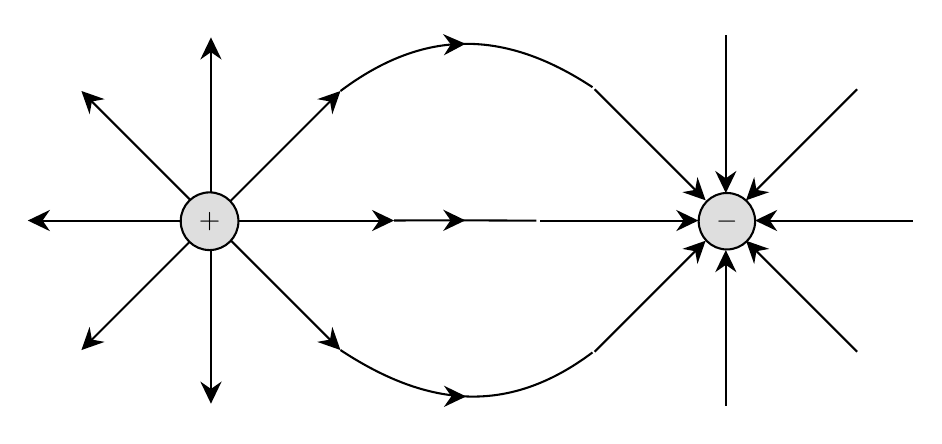
\begin{tikzpicture}[x=0.75pt,y=0.75pt,yscale=-1,xscale=1]
	%uncomment if require: \path (0,300); %set diagram left start at 0, and has height of 300

	%Straight Lines [id:da09226733946766874] 
	\draw    (168.42,159.42) -- (228.7,99.14) ;
	\draw [shift={(230.82,97.01)}, rotate = 495] [fill={rgb, 255:red, 0; green, 0; blue, 0 }  ][line width=0.08]  [draw opacity=0] (10.72,-5.15) -- (0,0) -- (10.72,5.15) -- (7.12,0) -- cycle    ;
	%Straight Lines [id:da7989832300210724] 
	\draw    (108.14,219.7) -- (168.42,159.42) ;
	\draw [shift={(106.01,221.82)}, rotate = 315] [fill={rgb, 255:red, 0; green, 0; blue, 0 }  ][line width=0.08]  [draw opacity=0] (10.72,-5.15) -- (0,0) -- (10.72,5.15) -- (7.12,0) -- cycle    ;
	%Straight Lines [id:da40069576982828825] 
	\draw    (168.42,159.42) -- (228.7,219.7) ;
	\draw [shift={(230.82,221.82)}, rotate = 225] [fill={rgb, 255:red, 0; green, 0; blue, 0 }  ][line width=0.08]  [draw opacity=0] (10.72,-5.15) -- (0,0) -- (10.72,5.15) -- (7.12,0) -- cycle    ;
	%Straight Lines [id:da5830973681811298] 
	\draw    (108.14,99.14) -- (168.42,159.42) ;
	\draw [shift={(106.01,97.01)}, rotate = 45] [fill={rgb, 255:red, 0; green, 0; blue, 0 }  ][line width=0.08]  [draw opacity=0] (10.72,-5.15) -- (0,0) -- (10.72,5.15) -- (7.12,0) -- cycle    ;
	%Straight Lines [id:da9186612483958567] 
	\draw    (168.42,159.42) -- (253.67,159.42) ;
	\draw [shift={(256.67,159.42)}, rotate = 180] [fill={rgb, 255:red, 0; green, 0; blue, 0 }  ][line width=0.08]  [draw opacity=0] (10.72,-5.15) -- (0,0) -- (10.72,5.15) -- (7.12,0) -- cycle    ;
	%Straight Lines [id:da6761948854902533] 
	\draw    (83.17,159.42) -- (168.42,159.42) ;
	\draw [shift={(80.17,159.42)}, rotate = 360] [fill={rgb, 255:red, 0; green, 0; blue, 0 }  ][line width=0.08]  [draw opacity=0] (10.72,-5.15) -- (0,0) -- (10.72,5.15) -- (7.12,0) -- cycle    ;
	%Straight Lines [id:da30542672054099773] 
	\draw    (168.42,159.42) -- (168.42,244.67) ;
	\draw [shift={(168.42,247.67)}, rotate = 270] [fill={rgb, 255:red, 0; green, 0; blue, 0 }  ][line width=0.08]  [draw opacity=0] (10.72,-5.15) -- (0,0) -- (10.72,5.15) -- (7.12,0) -- cycle    ;
	%Straight Lines [id:da9339624700136409] 
	\draw    (168.42,74.17) -- (168.42,159.42) ;
	\draw [shift={(168.42,71.17)}, rotate = 90] [fill={rgb, 255:red, 0; green, 0; blue, 0 }  ][line width=0.08]  [draw opacity=0] (10.72,-5.15) -- (0,0) -- (10.72,5.15) -- (7.12,0) -- cycle    ;
	%Straight Lines [id:da9122656922012751] 
	\draw    (428.34,147.56) -- (479.72,96.17) ;
	\draw [shift={(426.21,149.68)}, rotate = 315] [fill={rgb, 255:red, 0; green, 0; blue, 0 }  ][line width=0.08]  [draw opacity=0] (10.72,-5.15) -- (0,0) -- (10.72,5.15) -- (7.12,0) -- cycle    ;
	%Straight Lines [id:da33197275662358083] 
	\draw    (353.24,222.66) -- (404.62,171.27) ;
	\draw [shift={(406.75,169.15)}, rotate = 495] [fill={rgb, 255:red, 0; green, 0; blue, 0 }  ][line width=0.08]  [draw opacity=0] (10.72,-5.15) -- (0,0) -- (10.72,5.15) -- (7.12,0) -- cycle    ;
	%Straight Lines [id:da6193410325711912] 
	\draw    (428.34,171.27) -- (479.72,222.66) ;
	\draw [shift={(426.21,169.15)}, rotate = 45] [fill={rgb, 255:red, 0; green, 0; blue, 0 }  ][line width=0.08]  [draw opacity=0] (10.72,-5.15) -- (0,0) -- (10.72,5.15) -- (7.12,0) -- cycle    ;
	%Straight Lines [id:da3379499451012773] 
	\draw    (353.24,96.17) -- (404.62,147.56) ;
	\draw [shift={(406.75,149.68)}, rotate = 225] [fill={rgb, 255:red, 0; green, 0; blue, 0 }  ][line width=0.08]  [draw opacity=0] (10.72,-5.15) -- (0,0) -- (10.72,5.15) -- (7.12,0) -- cycle    ;
	%Straight Lines [id:da8633902170868257] 
	\draw    (433.58,159.42) -- (506.67,159.42) ;
	\draw [shift={(430.58,159.42)}, rotate = 0] [fill={rgb, 255:red, 0; green, 0; blue, 0 }  ][line width=0.08]  [draw opacity=0] (10.72,-5.15) -- (0,0) -- (10.72,5.15) -- (7.12,0) -- cycle    ;
	%Straight Lines [id:da6449899890477775] 
	\draw    (327.17,159.42) -- (400.25,159.42) ;
	\draw [shift={(403.25,159.42)}, rotate = 540] [fill={rgb, 255:red, 0; green, 0; blue, 0 }  ][line width=0.08]  [draw opacity=0] (10.72,-5.15) -- (0,0) -- (10.72,5.15) -- (7.12,0) -- cycle    ;
	%Straight Lines [id:da9631546207388431] 
	\draw    (416.48,176.65) -- (416.48,248.73) ;
	\draw [shift={(416.48,173.65)}, rotate = 90] [fill={rgb, 255:red, 0; green, 0; blue, 0 }  ][line width=0.08]  [draw opacity=0] (10.72,-5.15) -- (0,0) -- (10.72,5.15) -- (7.12,0) -- cycle    ;
	%Straight Lines [id:da3834974996926863] 
	\draw    (416.48,70.1) -- (416.48,143.19) ;
	\draw [shift={(416.48,146.19)}, rotate = 270] [fill={rgb, 255:red, 0; green, 0; blue, 0 }  ][line width=0.08]  [draw opacity=0] (10.72,-5.15) -- (0,0) -- (10.72,5.15) -- (7.12,0) -- cycle    ;
	%Curve Lines [id:da13623299495386587] 
	\draw    (230.82,97.01) .. controls (270.82,67.01) and (309.5,67) .. (352.24,95.17) ;
	\draw [shift={(291.1,74.27)}, rotate = 537.6700000000001] [fill={rgb, 255:red, 0; green, 0; blue, 0 }  ][line width=0.08]  [draw opacity=0] (10.72,-5.15) -- (0,0) -- (10.72,5.15) -- (7.12,0) -- cycle    ;
	%Curve Lines [id:da2452924867095878] 
	\draw    (256.67,159.42) .. controls (290.67,159.17) and (305,159.5) .. (325.17,159.42) ;
	\draw [shift={(290.99,159.34)}, rotate = 180.12] [fill={rgb, 255:red, 0; green, 0; blue, 0 }  ][line width=0.08]  [draw opacity=0] (10.72,-5.15) -- (0,0) -- (10.72,5.15) -- (7.12,0) -- cycle    ;
	%Curve Lines [id:da15092657275075516] 
	\draw    (352.24,222.98) .. controls (312.24,252.98) and (273.56,249.99) .. (230.82,221.82) ;
	\draw [shift={(291.35,244.17)}, rotate = 180.23] [fill={rgb, 255:red, 0; green, 0; blue, 0 }  ][line width=0.08]  [draw opacity=0] (10.72,-5.15) -- (0,0) -- (10.72,5.15) -- (7.12,0) -- cycle    ;

	% Text Node
	\draw  [fill={rgb, 255:red, 222; green, 222; blue, 222 }  ,fill opacity=1 ]  (167.75, 159.75) circle [x radius= 13.9, y radius= 13.9]   ;
	\draw (167.75,159.75) node    {$+$};
	% Text Node
	\draw  [fill={rgb, 255:red, 222; green, 222; blue, 222 }  ,fill opacity=1 ]  (417, 159.75) circle [x radius= 13.6, y radius= 13.6]   ;
	\draw (417,159.75) node    {$-$};

	\end{tikzpicture}
\end{figure}
\FloatBarrier

Supponendo che il campo vettoriale sia noto, possiamo procedere con questo ragionamento. Possiamo considerare un piccolo spostamento da $P$ a $P'$. Sostanzialmente $d\vec{r}$ si confonde con l'arco della linea di flusso. Mano a mano che $P'$ si avvicina $P$ diventa tangente all'andamento della linea. Questo vuol dire che possiamoc immaginare di rappresentare lo spostamento $d\vec{r}$ come:

\[
	\vec{r} = dx\vec{u}_x+dy\vec{u}_y+dz\vec{u}_z
\]

E se facciamo l'ipotesi che $V$ ed $\vec{r}$ sono paralleli, possiamo scrivere la similitudine tra le componenti di $V$ e le componenti di $\vec{r}$.

\[
	\boxed{\frac{dx}{V_x} = \frac{dy}{V_y} = \frac{dz}{V_z}}
\]

\section{Elementi di geometria e calcolo differenziale vettoriale}

\subsection{Angolo nel piano}
L'angolo nel piano è una parte di piano, delimitata da due semirette. Si definiscono i radianti come rapporto tra l'arco del cerchio e il raggio del cerchio.

\[
	\vartheta = \frac{l}{r} \; \implies \; \vartheta_{\text{giro}}  = \frac{2\pi r}{r} = 2\pi \;\; \text{(radianti)}
\]

\subsection{Angolo solido}
Possiamo immaginare di estendere il concetto di angolo nel piano alle tre dimensioni. Immaginiamo di tracciare un cono con vertice nel punto $O$. Tale cono, analogamente al caso del piano, delimita una porzione di spazio al suo interno. Immaginiamo di tracciare una sfera che abbia
centro coincidente in $O$. Dall'intersezione con il cono otterremo una calotta sferica di area $A$. Definiremo l'ampiezza dell'angolo solido come la quantità pari a questo rapporto:

\[
	\Omega = \frac{A}{r^2} \; \implies \; \Omega_{\text{giro}} = \frac{4\pi r^2}{r^2} =4\pi \;\; \text{(steradianti)}
\]

\begin{figure}[htpb]
	\centering

	\tikzset{every picture/.style={line width=0.75pt}} %set default line width to 0.75pt        

	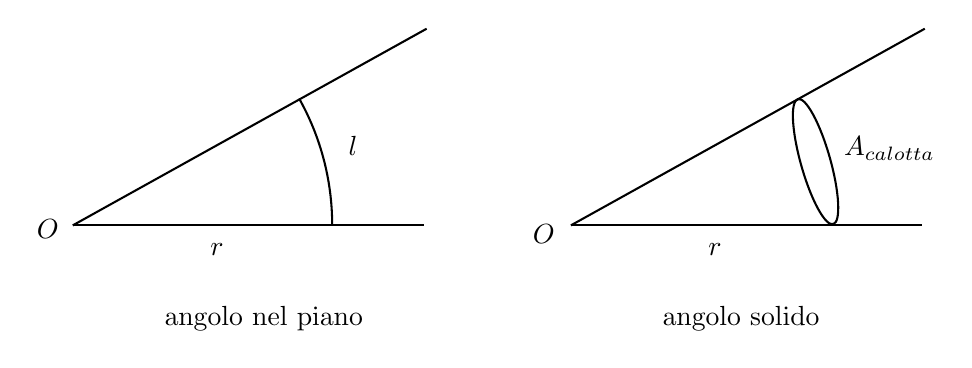
\begin{tikzpicture}[x=0.75pt,y=0.75pt,yscale=-1,xscale=1]
	%uncomment if require: \path (0,300); %set diagram left start at 0, and has height of 300

	%Straight Lines [id:da8133407336889511] 
	\draw    (69,187) -- (238,187) ;
	%Straight Lines [id:da9927555196654625] 
	\draw    (69,187) -- (239.5,92.25) ;
	%Shape: Arc [id:dp4648347309681775] 
	\draw  [draw opacity=0] (178.08,125.91) .. controls (188.18,143.91) and (193.96,164.66) .. (194,186.76) -- (69,187) -- cycle ; \draw   (178.08,125.91) .. controls (188.18,143.91) and (193.96,164.66) .. (194,186.76) ;
	%Straight Lines [id:da09140360982082418] 
	\draw    (309,187) -- (478,187) ;
	%Straight Lines [id:da1760952495285375] 
	\draw    (309,187) -- (479.5,92.25) ;
	%Shape: Ellipse [id:dp9119470894722195] 
	\draw   (418.37,126.17) .. controls (422.16,125.1) and (429.04,137.72) .. (433.74,154.35) .. controls (438.44,170.99) and (439.18,185.34) .. (435.4,186.41) .. controls (431.61,187.48) and (424.73,174.86) .. (420.03,158.23) .. controls (415.33,141.59) and (414.59,127.24) .. (418.37,126.17) -- cycle ;

	% Text Node
	\draw (204,148.5) node    {$l$};
	% Text Node
	\draw (138.5,198.5) node    {$r$};
	% Text Node
	\draw (462.5,150) node    {$A_{\text{calotta}}$};
	% Text Node
	\draw (378.5,198.5) node    {$r$};
	% Text Node
	\draw (161,232) node   [align=left] {angolo nel piano};
	% Text Node
	\draw (391,232) node   [align=left] {angolo solido};
	% Text Node
	\draw (57,189) node    {$O$};
	% Text Node
	\draw (296,191) node    {$O$};

	\end{tikzpicture}
\end{figure}
\FloatBarrier

Consideriamo un angolo solido di ampiezza infinitesima, $d\Omega$. Se consideriamo l'area intercettata dalla superficie sferica, essa sarà pari a:

\[
	A=d\Omega \, r^2
\]

Possiamo anche individuare la normale, il versore perpendicolare a questo tratto di superficie.

\begin{figure}[htpb]
	\centering

	\tikzset{every picture/.style={line width=0.75pt}} %set default line width to 0.75pt        

	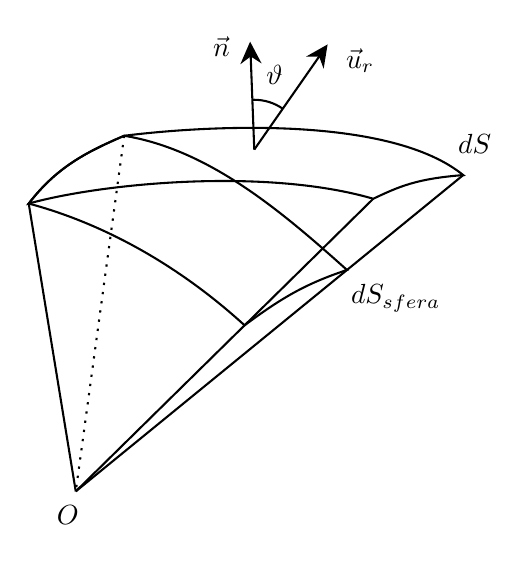
\begin{tikzpicture}[x=0.75pt,y=0.75pt,yscale=-1,xscale=1]
	%uncomment if require: \path (0,300); %set diagram left start at 0, and has height of 300

	%Shape: Polygon Curved [id:ds5242701370299456] 
	\draw   (216.33,82.67) .. controls (257,89.33) and (291.67,118.67) .. (323.67,147.33) .. controls (303.67,154) and (292.33,160.67) .. (274.33,174) .. controls (243.67,146) and (207.67,125.33) .. (170.33,115.33) .. controls (183.67,98) and (197.67,90.67) .. (216.33,82.67) -- cycle ;
	%Straight Lines [id:da719989530014286] 
	\draw    (170.33,115.33) -- (193,254) ;
	%Shape: Boxed Line [id:dp9909676259845537] 
	\draw    (379.67,101.62) -- (193,254) ;
	%Shape: Boxed Line [id:dp7130967066860716] 
	\draw    (336.33,113.02) -- (193,254) ;
	%Shape: Polygon Curved [id:ds5438868770758298] 
	\draw   (216.33,82.67) .. controls (259,77.33) and (345,73.33) .. (379.67,101.62) .. controls (357,103.33) and (348.33,107.33) .. (336.33,113.02) .. controls (285,98) and (206.33,105.33) .. (170.33,115.33) .. controls (183.67,98) and (197.67,90.67) .. (216.33,82.67) -- cycle ;
	%Straight Lines [id:da2179443455009622] 
	\draw  [dash pattern={on 0.84pt off 2.51pt}]  (216.33,82.67) -- (193,254) ;
	%Straight Lines [id:da03071624194168887] 
	\draw    (277.12,40.33) -- (279,89.33) ;
	\draw [shift={(277,37.33)}, rotate = 87.8] [fill={rgb, 255:red, 0; green, 0; blue, 0 }  ][line width=0.08]  [draw opacity=0] (10.72,-5.15) -- (0,0) -- (10.72,5.15) -- (7.12,0) -- cycle    ;
	%Straight Lines [id:da3105470001085451] 
	\draw    (312.62,41.13) -- (279,89.33) ;
	\draw [shift={(314.33,38.67)}, rotate = 124.89] [fill={rgb, 255:red, 0; green, 0; blue, 0 }  ][line width=0.08]  [draw opacity=0] (10.72,-5.15) -- (0,0) -- (10.72,5.15) -- (7.12,0) -- cycle    ;
	%Shape: Arc [id:dp11397532389152976] 
	\draw  [draw opacity=0] (278.09,65.35) .. controls (278.39,65.34) and (278.7,65.33) .. (279,65.33) .. controls (284.11,65.33) and (288.85,66.93) .. (292.74,69.65) -- (279,89.33) -- cycle ; \draw   (278.09,65.35) .. controls (278.39,65.34) and (278.7,65.33) .. (279,65.33) .. controls (284.11,65.33) and (288.85,66.93) .. (292.74,69.65) ;

	% Text Node
	\draw (263.2,39.8) node    {$\vec{n}$};
	% Text Node
	\draw (330,46.6) node    {$\vec{u}_{r}$};
	% Text Node
	\draw (288.8,53.4) node    {$\vartheta $};
	% Text Node
	\draw (347.2,161) node    {$dS_{\text{sfera}}$};
	% Text Node
	\draw (385.2,86.6) node    {$dS$};
	% Text Node
	\draw (189.2,265.6) node    {$O$};

	\end{tikzpicture}
\end{figure}
\FloatBarrier

Supponiamo che nella stessa zona ci sia una superficie non sferica ma di forma qualunque situata alla stessa distanza da $O$. Se proiettiamo la nuova superficie ds sulla sfera otterremo ds sfera. In formula:

\begin{align*}
	dS_{\text{sfera}} &= dS\,\cos \vartheta \\
	r^2 d\Omega &= dS\,\cos \vartheta \\
	r^2 d\Omega &= dS\,\vec{n} \cdot \vec{u}_r \\
	d\Omega &= \frac{dS\,\vec{n} \cdot \vec{u}_r}{r^2} \\
\end{align*}

\subsection{Le derivate parziali}

Supponiamo di avere una funzione $f=f(x,y,z)$.
Derivare parzialmente vuol dire mantenere costanti le altre variabili e far variare solo quella rispetto a cui stiamo derivando.

\[
	\boxed{\frac{\partial f}{\partial x} = \lim_{\Delta x \to 0} \frac{f(x+\Delta x,y,z)-f(x,y,z)}{\Delta x}}
\]
È possibile derivare una funzione $f(x,y,z)$ rispetto a ciascuna delle tre variabili, ottenendo quindi tre derivate parziali. La situazione si complica passando alle derivate di ordine superiore. Possiamo avere ad esempio la derivata seconda una volta rispetto a $x$ e una rispetto a $y$, oppure due volte rispetto a $x$ e via dicendo.

\subsection{Operatore Divergenza}

Il concetto di derivata parziale è necessario per introdurre l'operatore divergenza. Nel calcolo differenziale vettoriale, la divergenza è un campo scalare che misura la tendenza di un campo vettoriale a divergere o a convergere verso un punto dello spazio. Consideriamo il caso di un campo vettoriale $\vec{v} (P)$, funzione della posizione, definito in una certa regione dello spazio e in essa un punto $P$. Sia poi $\Sigma$ una superficie chiusa che lo circondi. Chiamiamo $\tau$ il volume racchiuso da essa. Definiamo la divergenza del vettore $\vec{v}$ in $P$ come:

\[
	\text{div}\vec{v} (P)=\lim_{\tau  \to 0} \frac{\Phi_{\Sigma}(\vec{v} )}{\tau}= \lim_{\tau  \to 0} \frac{\int_{\Sigma} \vec{v} \cdot \vec{n} dS}{\tau}
\]

che mappa un campo vettoriale in un campo scalare. Si dimostra inoltre che

\[
	\text{div}\vec{v} = \frac{\partial v_x}{\partial x} +\frac{\partial v_y}{\partial y} +\frac{\partial v_z}{\partial z}
\]

\subsection{Teorema della Divergenza}

Dato un campo $\vec{v}=\vec{v}(P)$ e $\Sigma$ una superficie chiusa di volume $\tau$, allora

\[
	\boxed{\Phi_{\Sigma}(\vec{v} ) = \int_{\Sigma}\vec{v} \cdot \vec{n} dS = \int_{\tau}(\text{div}\vec{v} )d\tau}
\]

Ossia ci mette in relazione integrali di superficie con integrali di volume.

L'idea alla base della dimostrazione è quella di pensare di suddividere
il volume in tanti cubetti infinitesimi e di calcolare la somma dei flussi.
I cubetti che sono dentro il volume hanno una faccia in comune. I flussi si cancellano a due a due e rimangono solo quelli attraverso la frontiera. Ecco perché la somma dei flussi sulla superficie esterna è uguale a quella sul volume.

Se non ci sono sorgenti, accade in genere che la divergenza del campo vettoriale è uguale a zero. Abbiamo infatti visto che tale operatore misura la tendenza del campo a convergere o a divergere in/da un punto. Immaginiamo due linee chiuse $\Gamma_1$ e $\Gamma_2$ e le varie linee di flusso del campo che passano per esse. Supponiamo che la divergenza del campo $\vec{v}$ in questa regione sia nulla.

\begin{figure}[htpb]
	\centering

	\tikzset{every picture/.style={line width=0.75pt}} %set default line width to 0.75pt        

	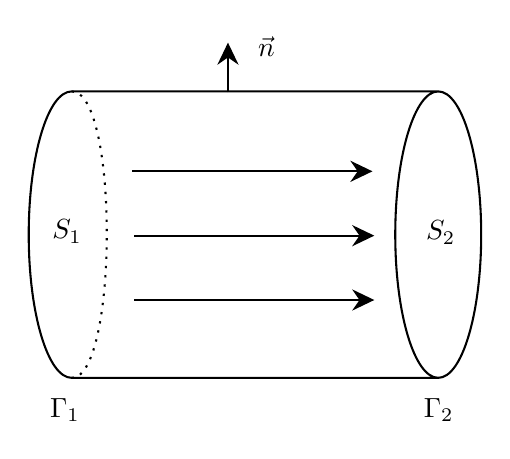
\begin{tikzpicture}[x=0.75pt,y=0.75pt,yscale=-1,xscale=1]
	%uncomment if require: \path (0,300); %set diagram left start at 0, and has height of 300

	%Shape: Can [id:dp07821714761930187] 
	\draw   (345.3,235.5) -- (168.7,235.5) .. controls (157.27,235.5) and (148,204.61) .. (148,166.5) .. controls (148,128.39) and (157.27,97.5) .. (168.7,97.5) -- (345.3,97.5) .. controls (356.73,97.5) and (366,128.39) .. (366,166.5) .. controls (366,204.61) and (356.73,235.5) .. (345.3,235.5) .. controls (333.87,235.5) and (324.6,204.61) .. (324.6,166.5) .. controls (324.6,128.39) and (333.87,97.5) .. (345.3,97.5) ;
	%Straight Lines [id:da819729350698617] 
	\draw    (198.88,198) -- (311.5,198) ;
	\draw [shift={(314.5,198)}, rotate = 180] [fill={rgb, 255:red, 0; green, 0; blue, 0 }  ][line width=0.08]  [draw opacity=0] (10.72,-5.15) -- (0,0) -- (10.72,5.15) -- (7.12,0) -- cycle    ;
	%Straight Lines [id:da13329799845494272] 
	\draw    (244,98) -- (244,77) ;
	\draw [shift={(244,74)}, rotate = 450] [fill={rgb, 255:red, 0; green, 0; blue, 0 }  ][line width=0.08]  [draw opacity=0] (10.72,-5.15) -- (0,0) -- (10.72,5.15) -- (7.12,0) -- cycle    ;
	%Straight Lines [id:da6320350854720245] 
	\draw    (198.88,167) -- (311.5,167) ;
	\draw [shift={(314.5,167)}, rotate = 180] [fill={rgb, 255:red, 0; green, 0; blue, 0 }  ][line width=0.08]  [draw opacity=0] (10.72,-5.15) -- (0,0) -- (10.72,5.15) -- (7.12,0) -- cycle    ;
	%Straight Lines [id:da09893112591978959] 
	\draw    (198,136) -- (310.62,136) ;
	\draw [shift={(313.62,136)}, rotate = 180] [fill={rgb, 255:red, 0; green, 0; blue, 0 }  ][line width=0.08]  [draw opacity=0] (10.72,-5.15) -- (0,0) -- (10.72,5.15) -- (7.12,0) -- cycle    ;
	%Curve Lines [id:da7589395231546388] 
	\draw  [dash pattern={on 0.84pt off 2.51pt}]  (168.7,97.5) .. controls (191.5,97.25) and (191,235.75) .. (168.7,235.5) ;

	% Text Node
	\draw (262.5,76) node    {$\vec{n}$};
	% Text Node
	\draw (166.5,165) node    {$S_{1}$};
	% Text Node
	\draw (346.5,165.5) node    {$S_{2}$};
	% Text Node
	\draw (165.5,251) node    {$\Gamma _{1}$};
	% Text Node
	\draw (345.5,251) node    {$\Gamma _{2}$};

	\end{tikzpicture}
\end{figure}
\FloatBarrier

L'inviluppo di queste linee da vita a una superficie chiusa che chiamiamo \textbf{superficie di flusso} (parallela alla linee di flusso).
Immaginiamo di considerare il cilindro dato dal tubo di flusso e le due aree di base racchiuse dalle due linee $\Gamma_1$ e $\Gamma_2$. Se vogliamo calcolare il flusso del campo vettoriale attraverso quella superficie chiusa, questo flusso totale sarà la somma di tre contributi: il flusso sulla superficie laterale del tubo, il flusso attraverso la superficie $S_1$ e il flusso attraverso la superficie $S_2$, chiusa dall'altra linea. Se in quella regione la divergenza è uguale a zero il flusso totale è uguale a zero.

\[
	\Phi_{\text{tot}}(\vec{v} ) = \Phi_{\Sigma}(\vec{v}) + \Phi_{S_1}(\vec{v}) + \Phi_{S_2}(\vec{v})
\]

Siccome la superficie considerata è costituita dalle linee di flusso, il vettore normale è perpendicolare a $\vec{v}$ e anche il flusso attraverso la superficie laterale è uguale a zero.
Questo ci dice che il flusso attraverso la superficie $S_1$ è uguale all'opposto di quello che attraversa la sezione $S_2$.

\[
	|\Phi_{S_1}(\vec{v})| = |\Phi_{S_2}(\vec{v})|
\]

Il risultato che abbiamo ottenuto è che in una regione in cui la divergenza è uguale a zero, il flusso del il campo vettoriale attraverso il tubo di flusso rimane costante.

\subsection{Operatore Rotore}

Sia $ \vec{v} =\vec{v} (P) $ un campo vettoriale definito in un dominio semplicemente connesso. Denotiamo $\vec{w} = \text{rot}\vec{v} (P)$.
Sia $\gamma$ una linea chiusa orientata che circonda $P$, sia $\Sigma$ una superficie di area $S$ avente $\gamma$ come contorno e passi per il punto $P$. Sia $\vec{n}$ il versore normale alla superficie, con verso scelto con la regola del cavatappi.

\begin{figure}[htpb]
	\centering

	\tikzset{every picture/.style={line width=0.75pt}} %set default line width to 0.75pt        

	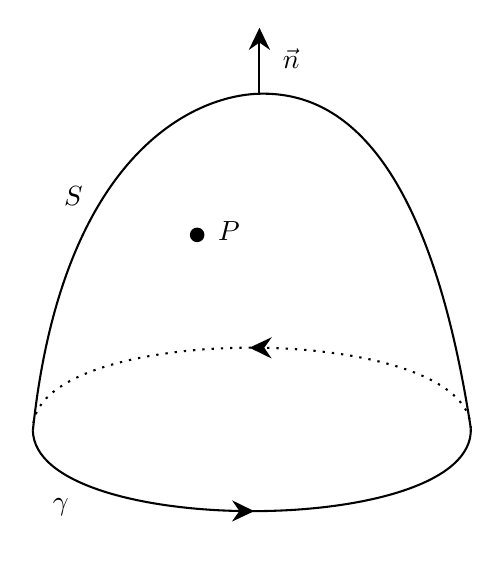
\begin{tikzpicture}[x=0.75pt,y=0.75pt,yscale=-1,xscale=1]
	%uncomment if require: \path (0,300); %set diagram left start at 0, and has height of 300

	%Curve Lines [id:da2720989042066049] 
	\draw    (154.5,220) .. controls (155.5,272) and (367.5,272) .. (365.5,219) ;
	\draw [shift={(261.13,258.88)}, rotate = 180.43] [fill={rgb, 255:red, 0; green, 0; blue, 0 }  ][line width=0.08]  [draw opacity=0] (10.72,-5.15) -- (0,0) -- (10.72,5.15) -- (7.12,0) -- cycle    ;
	%Curve Lines [id:da9383416644738221] 
	\draw  [dash pattern={on 0.84pt off 2.51pt}]  (365.5,219) .. controls (364.5,167) and (152.5,167) .. (154.5,220) ;
	\draw [shift={(258.87,180.13)}, rotate = 360.43] [fill={rgb, 255:red, 0; green, 0; blue, 0 }  ][line width=0.08]  [draw opacity=0] (10.72,-5.15) -- (0,0) -- (10.72,5.15) -- (7.12,0) -- cycle    ;
	%Shape: Circle [id:dp49398570007450715] 
	\draw  [fill={rgb, 255:red, 0; green, 0; blue, 0 }  ,fill opacity=1 ] (230.66,125.77) .. controls (230.66,124.12) and (232,122.77) .. (233.66,122.77) .. controls (235.32,122.77) and (236.66,124.12) .. (236.66,125.77) .. controls (236.66,127.43) and (235.32,128.77) .. (233.66,128.77) .. controls (232,128.77) and (230.66,127.43) .. (230.66,125.77) -- cycle ;
	%Straight Lines [id:da032901312924457526] 
	\draw    (263.66,29) -- (263.66,57.77) ;
	\draw [shift={(263.66,26)}, rotate = 90] [fill={rgb, 255:red, 0; green, 0; blue, 0 }  ][line width=0.08]  [draw opacity=0] (10.72,-5.15) -- (0,0) -- (10.72,5.15) -- (7.12,0) -- cycle    ;
	%Curve Lines [id:da9435042530698341] 
	\draw    (154.5,220) .. controls (168.5,87) and (231.82,58.55) .. (263.66,57.77) .. controls (295.5,57) and (343.5,76) .. (365.5,219) ;

	% Text Node
	\draw (174,107) node    {$S$};
	% Text Node
	\draw (249,124) node    {$P$};
	% Text Node
	\draw (279,41) node    {$\vec{n}$};
	% Text Node
	\draw (168,257) node    {$\gamma $};

	\end{tikzpicture}
\end{figure}
\FloatBarrier

Si definisce

\[
	(\text{rot}\vec{v} )\cdot (\vec{n} )= \lim_{S \to 0} \frac{\oint_{\gamma} \vec{v} \cdot d\vec{l}}{S}
\]

Essendo $ \vec{v} = v_x\vec{u}_x +v_y\vec{u}_y + v_z\vec{u}_z    $ si dimostra che che

\[
	\vec{w} = \text{rot}\vec{v} = \begin{vmatrix}
		\vec{u}_x & \vec{u}_y & \vec{u}_z \\
		\frac{\partial}{\partial x} & \frac{\partial}{\partial y} & \frac{\partial}{\partial z}  \\
		v_x & v_y & v_z
	\end{vmatrix}
\]

\[
	\vec{w} = \text{rot}\vec{v} = \vec{u}_x\left( \frac{\partial v_z}{\partial y} -\frac{\partial v_y}{\partial z}  \right)  +
	\vec{u}_y\left( \frac{\partial v_x}{\partial z} -\frac{\partial v_z}{\partial x}  \right)  +
	\vec{u}_z\left( \frac{\partial v_y}{\partial x} -\frac{\partial v_x}{\partial y}  \right)
\]

\subsection{Teorema di Stokes}

Il passaggio ad una linea chiusa finita è garantito dal teorema di Stokes. Supponiamo di aver definito un campo vettoriale $\vec{v}(P)$ funzione della posizione in un certo dominio semplicemente connesso (data una linea chiusa è sempre possibile trovare almeno una superficie contenuta interamente nel dominio e avente la linea come contorno). Immaginiamo di definire in questa regione una linea chiusa $\gamma$ orientata che abbia una superficie $\Sigma$ aperta di cui costituisce il contorno.

\begin{figure}[htpb]
	\centering

	\tikzset{every picture/.style={line width=0.75pt}} %set default line width to 0.75pt        

	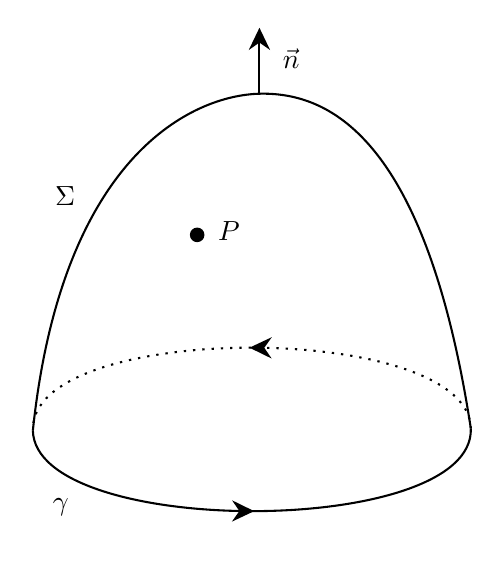
\begin{tikzpicture}[x=0.75pt,y=0.75pt,yscale=-1,xscale=1]
	%uncomment if require: \path (0,300); %set diagram left start at 0, and has height of 300

	%Curve Lines [id:da15583153412401485] 
	\draw    (164.5,218) .. controls (165.5,270) and (377.5,270) .. (375.5,217) ;
	\draw [shift={(271.13,256.88)}, rotate = 180.43] [fill={rgb, 255:red, 0; green, 0; blue, 0 }  ][line width=0.08]  [draw opacity=0] (10.72,-5.15) -- (0,0) -- (10.72,5.15) -- (7.12,0) -- cycle    ;
	%Curve Lines [id:da5672800465241312] 
	\draw  [dash pattern={on 0.84pt off 2.51pt}]  (375.5,217) .. controls (374.5,165) and (162.5,165) .. (164.5,218) ;
	\draw [shift={(268.87,178.13)}, rotate = 360.43] [fill={rgb, 255:red, 0; green, 0; blue, 0 }  ][line width=0.08]  [draw opacity=0] (10.72,-5.15) -- (0,0) -- (10.72,5.15) -- (7.12,0) -- cycle    ;
	%Shape: Circle [id:dp2951783555532528] 
	\draw  [fill={rgb, 255:red, 0; green, 0; blue, 0 }  ,fill opacity=1 ] (240.66,123.77) .. controls (240.66,122.12) and (242,120.77) .. (243.66,120.77) .. controls (245.32,120.77) and (246.66,122.12) .. (246.66,123.77) .. controls (246.66,125.43) and (245.32,126.77) .. (243.66,126.77) .. controls (242,126.77) and (240.66,125.43) .. (240.66,123.77) -- cycle ;
	%Straight Lines [id:da6906371612066755] 
	\draw    (273.66,27) -- (273.66,55.77) ;
	\draw [shift={(273.66,24)}, rotate = 90] [fill={rgb, 255:red, 0; green, 0; blue, 0 }  ][line width=0.08]  [draw opacity=0] (10.72,-5.15) -- (0,0) -- (10.72,5.15) -- (7.12,0) -- cycle    ;
	%Curve Lines [id:da12239522891457866] 
	\draw    (164.5,218) .. controls (178.5,85) and (241.82,56.55) .. (273.66,55.77) .. controls (305.5,55) and (353.5,74) .. (375.5,217) ;

	% Text Node
	\draw (180,105) node    {$\Sigma $};
	% Text Node
	\draw (259,122) node    {$P$};
	% Text Node
	\draw (289,39) node    {$\vec{n}$};
	% Text Node
	\draw (178,255) node    {$\gamma $};

	\end{tikzpicture}
\end{figure}
\FloatBarrier

Scegliamo sulla superficie il verso della normale $\vec{n}$,
diretta verso l'alto, in accordo con la regola del cavatappi. Il teorema afferma che la circuitazione di un campo vettoriale lungo una linea chiusa $\gamma$ è uguale al flusso del rotore del campo attraverso una \emph{qualunque} superficie $\Sigma$ avente come contorno $\gamma$.

\[
	\boxed{\oint_{\gamma} \vec{v} \cdot d\vec{l} = \int_{\Sigma}(\text{rot}\vec{v} )\cdot \vec{n} dS}
\]

Mette in relazione un integrale di linea, con un integrale di superficie.

\subsection{Operatore Nabla}

Si può introdurre il vettore simbolico $ \vec{\nabla}  $ definito come:

\[
	\vec{\nabla} = \vec{u}_x \frac{\partial}{\partial x} + \vec{u}_y \frac{\partial}{\partial y} + \vec{u}_z \frac{\partial}{\partial z}
\]

per scrivere la divergenza come

\[
	\text{div}\vec{v} = \vec{\nabla} \cdot \vec{v}  = \frac{\partial v_x}{\partial x} + \frac{\partial v_y}{\partial y} + \frac{\partial v_z}{\partial z}
\]

e analogamente il rotore come

\[
	\text{rot}\vec{v} = \vec{\nabla} \times  \vec{v}  = \left(
	\frac{\partial v_z}{\partial y} -\frac{\partial v_y}{\partial z},
	\frac{\partial v_x}{\partial z} -\frac{\partial v_z}{\partial x},
	\frac{\partial v_y}{\partial x} -\frac{\partial v_x}{\partial y} \right)
\]

\subsection{Flusso di un campo vettoriale}

Supponiamo che in una regione di spazio sia definito un campo vettoriale e individuata una superficie $\Sigma$. Nel punto $P$ individuiamo un quadrettino di area infinitesima $dS$. Sia $\vec{n}$ la normale alla superficie. Definiremo flusso elementare di $\vec{v}(P)$ attraverso l'area infinitesima $dS$ la quantità $d\Phi$.

\[
	\boxed{d\Phi (\vec{v}) = \vec{v} (P)\cdot \vec{n} \,dS}
\]

Possiamo estendere la definizione di flusso all'intera superficie $\Sigma$. Infatti posso immaginarla come divisa da quadretti di area infinitesima e calcolare il flusso in ognuno di essi, andando a sommare poi queste quantità.

\begin{figure}[htpb]
	\centering

	\tikzset{every picture/.style={line width=0.75pt}} %set default line width to 0.75pt        

	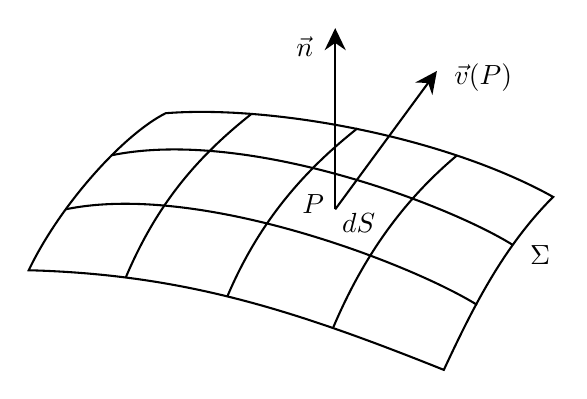
\begin{tikzpicture}[x=0.75pt,y=0.75pt,yscale=-1,xscale=1]
	%uncomment if require: \path (0,300); %set diagram left start at 0, and has height of 300

	%Shape: Polygon Curved [id:ds8769549835569137] 
	\draw   (228.33,69.67) .. controls (279,65.67) and (362.33,80.67) .. (415,110) .. controls (391,134) and (376.33,163.33) .. (362.33,193.33) .. controls (289,164) and (236.33,147.33) .. (162.33,145.33) .. controls (177.67,113.33) and (208.33,79.67) .. (228.33,69.67) -- cycle ;
	%Curve Lines [id:da563805179515227] 
	\draw    (209,149) .. controls (223,116) and (241,92.67) .. (269.67,70) ;
	%Curve Lines [id:da05137663634575418] 
	\draw    (258,158) .. controls (272,125) and (292,99.67) .. (320.67,77) ;
	%Curve Lines [id:da44819172214290304] 
	\draw    (309,173) .. controls (323,140) and (341.67,112.67) .. (368.67,90) ;
	%Curve Lines [id:da47225998773408695] 
	\draw    (202,90) .. controls (266,76.67) and (363,113) .. (395.33,133) ;
	%Curve Lines [id:da6171027402669229] 
	\draw    (180,116) .. controls (244,102.67) and (346,142) .. (378.33,162) ;
	%Straight Lines [id:da9267137414829982] 
	\draw    (310,116) -- (310,31.67) ;
	\draw [shift={(310,28.67)}, rotate = 450] [fill={rgb, 255:red, 0; green, 0; blue, 0 }  ][line width=0.08]  [draw opacity=0] (10.72,-5.15) -- (0,0) -- (10.72,5.15) -- (7.12,0) -- cycle    ;
	%Straight Lines [id:da934350194093134] 
	\draw    (310,116) -- (357.22,51.75) ;
	\draw [shift={(359,49.33)}, rotate = 486.32] [fill={rgb, 255:red, 0; green, 0; blue, 0 }  ][line width=0.08]  [draw opacity=0] (10.72,-5.15) -- (0,0) -- (10.72,5.15) -- (7.12,0) -- cycle    ;

	% Text Node
	\draw (381.33,52.33) node    {$\vec{v}( P)$};
	% Text Node
	\draw (295.33,37.67) node    {$\vec{n}$};
	% Text Node
	\draw (321.33,122.67) node    {$dS$};
	% Text Node
	\draw (299.33,113.33) node    {$P$};
	% Text Node
	\draw (408.67,138) node    {$\Sigma $};

	\end{tikzpicture}
\end{figure}
\FloatBarrier

Il flusso del campo vettoriale $\vec{v}(P)$ attraverso la superficie $\Sigma$ sarà:

\[
	\Phi_{\Sigma}(\vec{v} ) = \int_{\tau}d\Phi (\vec{v} )=\int_{\Sigma}\vec{v} \cdot \vec{n} \,dS
\]

Il nome di flusso deriva dalle applicazioni in idrodinamica, ma deve essere chiaro che il flusso di un campo vettoriale è un concetto matematico e non si accompagna necessariamente al passaggio attraverso $\Sigma$ di materia o di energia.

Nel caso di una superficie chiusa si assume che la normale sia diretta sempre verso l'esterno della superficie stessa. Supponiamo che in tal caso il campo vettoriale di cui ci stiamo occupando sia diretto anche lui verso l'esterno. Quello che risulta è che l'angolo che $\vec{v}$ ed $\vec{n}$ formano in genere è un angolo acuto. Il prodotto scalare fra $\vec{n}$ e $\vec{v}$ sarà positivo. Ecco perché allora il flusso positivo è un \textbf{flusso uscente}. Viceversa se il nostro campo vettoriale è diretto verso l'interno della superficie, allora in questo caso l'angolo che $\vec{v}$ ed $\vec{n}$ formano è ottuso e il flusso sarà negativo, diremo che sarà un \textbf{flusso entrante}.

\begin{figure}[htpb]
	\centering

	\tikzset{every picture/.style={line width=0.75pt}} %set default line width to 0.75pt        

	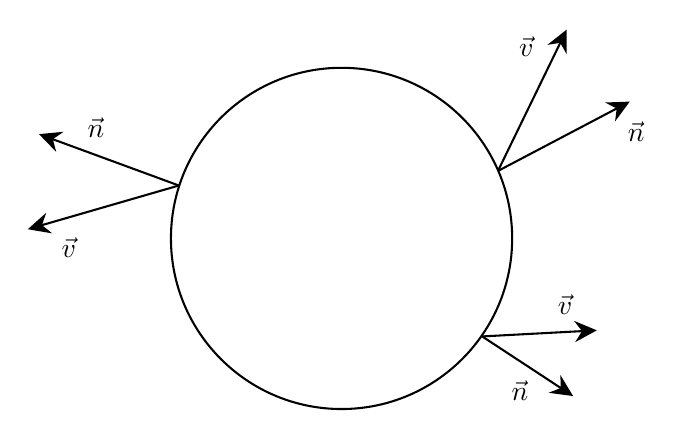
\begin{tikzpicture}[x=0.75pt,y=0.75pt,yscale=-1,xscale=1]
	%uncomment if require: \path (0,300); %set diagram left start at 0, and has height of 300

	%Shape: Ellipse [id:dp8770968669765249] 
	\draw   (152.31,148.29) .. controls (152.31,102.89) and (189.11,66.09) .. (234.51,66.09) .. controls (279.91,66.09) and (316.71,102.89) .. (316.71,148.29) .. controls (316.71,193.69) and (279.91,230.5) .. (234.51,230.5) .. controls (189.11,230.5) and (152.31,193.69) .. (152.31,148.29) -- cycle ;
	%Straight Lines [id:da7209345608057556] 
	\draw    (309.86,115.8) -- (341.69,50.36) ;
	\draw [shift={(343,47.66)}, rotate = 475.94] [fill={rgb, 255:red, 0; green, 0; blue, 0 }  ][line width=0.08]  [draw opacity=0] (10.72,-5.15) -- (0,0) -- (10.72,5.15) -- (7.12,0) -- cycle    ;
	%Straight Lines [id:da7804379502263452] 
	\draw    (309.86,115.8) -- (370.73,83.78) ;
	\draw [shift={(373.38,82.38)}, rotate = 512.26] [fill={rgb, 255:red, 0; green, 0; blue, 0 }  ][line width=0.08]  [draw opacity=0] (10.72,-5.15) -- (0,0) -- (10.72,5.15) -- (7.12,0) -- cycle    ;
	%Straight Lines [id:da6934703276913838] 
	\draw    (156.12,122.81) -- (86.22,143.04) ;
	\draw [shift={(83.34,143.88)}, rotate = 343.86] [fill={rgb, 255:red, 0; green, 0; blue, 0 }  ][line width=0.08]  [draw opacity=0] (10.72,-5.15) -- (0,0) -- (10.72,5.15) -- (7.12,0) -- cycle    ;
	%Straight Lines [id:da13641523911734055] 
	\draw    (156.12,122.81) -- (91.56,99.09) ;
	\draw [shift={(88.74,98.06)}, rotate = 380.18] [fill={rgb, 255:red, 0; green, 0; blue, 0 }  ][line width=0.08]  [draw opacity=0] (10.72,-5.15) -- (0,0) -- (10.72,5.15) -- (7.12,0) -- cycle    ;
	%Straight Lines [id:da8265055914518438] 
	\draw    (302.28,195.52) -- (354.49,192.74) ;
	\draw [shift={(357.49,192.58)}, rotate = 536.96] [fill={rgb, 255:red, 0; green, 0; blue, 0 }  ][line width=0.08]  [draw opacity=0] (10.72,-5.15) -- (0,0) -- (10.72,5.15) -- (7.12,0) -- cycle    ;
	%Straight Lines [id:da12763025741024703] 
	\draw    (302.28,195.52) -- (343.56,222.61) ;
	\draw [shift={(346.07,224.25)}, rotate = 213.28] [fill={rgb, 255:red, 0; green, 0; blue, 0 }  ][line width=0.08]  [draw opacity=0] (10.72,-5.15) -- (0,0) -- (10.72,5.15) -- (7.12,0) -- cycle    ;

	% Text Node
	\draw (323.51,55.97) node    {$\vec{v}$};
	% Text Node
	\draw (376.43,96.6) node    {$\vec{n}$};
	% Text Node
	\draw (320.47,221.53) node    {$\vec{n}$};
	% Text Node
	\draw (116.16,94.87) node    {$\vec{n}$};
	% Text Node
	\draw (342.16,180.03) node    {$\vec{v}$};
	% Text Node
	\draw (103.14,152.7) node    {$\vec{v}$};

	\end{tikzpicture}
\end{figure}
\FloatBarrier

Supponiamo ancora una volta di avere un campo vettoriale in una regione di spazio e di avere una linea chiusa $\Gamma$. Disegniamo soltanto quelle particolari linee di flusso che passano per la linea $\Gamma$. Otterremo una superficie tubolare individuata da tutte le linee che passano per tale linea.

\begin{figure}[htpb]
	\centering

	\tikzset{every picture/.style={line width=0.75pt}} %set default line width to 0.75pt        

	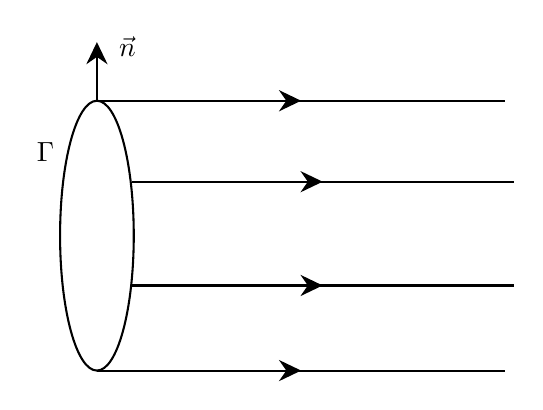
\begin{tikzpicture}[x=0.75pt,y=0.75pt,yscale=-1,xscale=1]
	%uncomment if require: \path (0,300); %set diagram left start at 0, and has height of 300

	%Shape: Ellipse [id:dp021868135678277723] 
	\draw   (108,138) .. controls (108,102.1) and (115.95,73) .. (125.75,73) .. controls (135.55,73) and (143.5,102.1) .. (143.5,138) .. controls (143.5,173.9) and (135.55,203) .. (125.75,203) .. controls (115.95,203) and (108,173.9) .. (108,138) -- cycle ;
	%Straight Lines [id:da0013832645143680988] 
	\draw    (125.75,73) -- (322.5,73) ;
	\draw [shift={(224.13,73)}, rotate = 180] [fill={rgb, 255:red, 0; green, 0; blue, 0 }  ][line width=0.08]  [draw opacity=0] (10.72,-5.15) -- (0,0) -- (10.72,5.15) -- (7.12,0) -- cycle    ;
	%Straight Lines [id:da09557240360638342] 
	\draw    (125.75,203) -- (322.5,203) ;
	\draw [shift={(224.13,203)}, rotate = 180] [fill={rgb, 255:red, 0; green, 0; blue, 0 }  ][line width=0.08]  [draw opacity=0] (10.72,-5.15) -- (0,0) -- (10.72,5.15) -- (7.12,0) -- cycle    ;
	%Straight Lines [id:da3950416933849661] 
	\draw    (142.5,162) -- (326.5,162) ;
	\draw [shift={(234.5,162)}, rotate = 180] [fill={rgb, 255:red, 0; green, 0; blue, 0 }  ][line width=0.08]  [draw opacity=0] (10.72,-5.15) -- (0,0) -- (10.72,5.15) -- (7.12,0) -- cycle    ;
	%Straight Lines [id:da7389004927289446] 
	\draw    (142.5,112) -- (326.5,112) ;
	\draw [shift={(234.5,112)}, rotate = 180] [fill={rgb, 255:red, 0; green, 0; blue, 0 }  ][line width=0.08]  [draw opacity=0] (10.72,-5.15) -- (0,0) -- (10.72,5.15) -- (7.12,0) -- cycle    ;
	%Straight Lines [id:da14730215659138457] 
	\draw    (125.75,73) -- (125.75,47.75) ;
	\draw [shift={(125.75,44.75)}, rotate = 450] [fill={rgb, 255:red, 0; green, 0; blue, 0 }  ][line width=0.08]  [draw opacity=0] (10.72,-5.15) -- (0,0) -- (10.72,5.15) -- (7.12,0) -- cycle    ;

	% Text Node
	\draw (101,97.5) node    {$\Gamma $};
	% Text Node
	\draw (140.5,47) node    {$\vec{n}$};

	\end{tikzpicture}
\end{figure}
\FloatBarrier

Questo tubo che abbiamo individuato prende il nome di \textbf{tubo di flusso}. La normale alla superficie sarà perpendicolare a $\vec{v}$ e il prodotto scalare fra $\vec{v}$ ed $\vec{n}$ è nullo.

\section{Teorema di Gauss per il campo elettrico}

Possiamo ora enunciare e dimostrare il teorema di Gauss per il campo elettrico.

\begin{figure}[htpb]
	\centering

	\tikzset{every picture/.style={line width=0.75pt}} %set default line width to 0.75pt        

	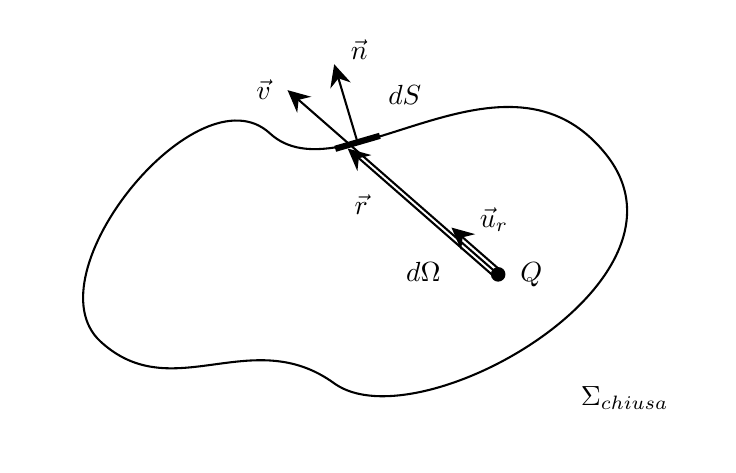
\begin{tikzpicture}[x=0.75pt,y=0.75pt,yscale=-1,xscale=1]
	%uncomment if require: \path (0,300); %set diagram left start at 0, and has height of 300

	%Shape: Polygon Curved [id:ds8897561476684546] 
	\draw   (396.59,96.87) .. controls (444.84,157.59) and (305.5,236) .. (265.5,207) .. controls (225.5,178) and (187.41,218.67) .. (152.86,186.81) .. controls (118.32,154.95) and (199.95,54.69) .. (234.5,86.55) .. controls (269.04,118.41) and (348.34,36.15) .. (396.59,96.87) -- cycle ;
	%Straight Lines [id:da27415252737009266] 
	\draw [line width=2.25]    (266,94) -- (287.5,87.75) ;
	%Straight Lines [id:da5060852752682012] 
	\draw    (245.26,67.72) -- (344.5,154.5) ;
	\draw [shift={(243,65.75)}, rotate = 41.17] [fill={rgb, 255:red, 0; green, 0; blue, 0 }  ][line width=0.08]  [draw opacity=0] (10.72,-5.15) -- (0,0) -- (10.72,5.15) -- (7.12,0) -- cycle    ;
	%Shape: Circle [id:dp03455482329752391] 
	\draw  [fill={rgb, 255:red, 0; green, 0; blue, 0 }  ,fill opacity=1 ] (341.5,154.5) .. controls (341.5,152.84) and (342.84,151.5) .. (344.5,151.5) .. controls (346.16,151.5) and (347.5,152.84) .. (347.5,154.5) .. controls (347.5,156.16) and (346.16,157.5) .. (344.5,157.5) .. controls (342.84,157.5) and (341.5,156.16) .. (341.5,154.5) -- cycle ;
	%Straight Lines [id:da5400783698484286] 
	\draw    (324.26,133.93) -- (345.5,152.5) ;
	\draw [shift={(322,131.95)}, rotate = 41.17] [fill={rgb, 255:red, 0; green, 0; blue, 0 }  ][line width=0.08]  [draw opacity=0] (10.72,-5.15) -- (0,0) -- (10.72,5.15) -- (7.12,0) -- cycle    ;
	%Straight Lines [id:da5326366958895112] 
	\draw    (274.26,95.83) -- (342.5,155.5) ;
	\draw [shift={(272,93.86)}, rotate = 41.17] [fill={rgb, 255:red, 0; green, 0; blue, 0 }  ][line width=0.08]  [draw opacity=0] (10.72,-5.15) -- (0,0) -- (10.72,5.15) -- (7.12,0) -- cycle    ;
	%Straight Lines [id:da6906937215964353] 
	\draw    (266.36,56.12) -- (276.75,90.88) ;
	\draw [shift={(265.5,53.25)}, rotate = 73.35] [fill={rgb, 255:red, 0; green, 0; blue, 0 }  ][line width=0.08]  [draw opacity=0] (10.72,-5.15) -- (0,0) -- (10.72,5.15) -- (7.12,0) -- cycle    ;

	% Text Node
	\draw (299.5,68) node    {$dS$};
	% Text Node
	\draw (360.5,154.5) node    {$Q$};
	% Text Node
	\draw (342.5,128) node    {$\vec{u}_{r}$};
	% Text Node
	\draw (278.5,121) node    {$\vec{r}$};
	% Text Node
	\draw (231.5,65.5) node    {$\vec{v}$};
	% Text Node
	\draw (277.5,46) node    {$\vec{n}$};
	% Text Node
	\draw (308.5,153.5) node    {$d\Omega $};
	% Text Node
	\draw (405.5,214) node    {$\Sigma _{\text{chiusa}}$};

	\end{tikzpicture}
\end{figure}
\FloatBarrier

Siano:

\begin{itemize}
	\item $\Sigma$ una superficie chiusa di forma qualunque
	\item La carica $Q$ dentro $\Sigma$
	\item $d\Omega$ l'angolo solido infinitesimo che individua $dS$
	\item $\vec{u}_r$ il versore radiale
\end{itemize}

Sostituendo l'espressione $ \vec{E} =\frac{Q\vec{u}_r}{4\pi \varepsilon_0r^2} $ nel flusso infinitesimo $ d\Phi(\vec{E} ) =\vec{E} \cdot \vec{n} dS$ si ottiene

\[
	d\Phi(\vec{E} )=\frac{Q}{4\pi \varepsilon_0}\left( \frac{\vec{u}_r\vec{n} dS}{r^2} \right)  = \frac{Q}{4\pi \varepsilon_0} d\Omega
\]

Integrando

\[
	\Phi_{\Sigma}(\vec{E} )=\int_{\Sigma}d\Phi=\int_{\Sigma} \frac{Q}{4\pi\varepsilon_0} d\Omega = \frac{Q}{4\pi \varepsilon_0} \int_{\Sigma} d\Omega = \frac{Q}{4\pi \varepsilon_0} \cdot 4\pi = \frac{Q}{\varepsilon_0}
\]

Quindi il flusso non dipende da $\Sigma$.

Siamo riusciti a fare questa semplificazione perché il campo elettrico decresce con il quadrato della distanza ed è diretto proprio in direzione radiale. Per tutti i campi che hanno queste proprietà si può definire un teorema di Gauss analogo. Viceversa, per un campo radiale qualunque del tipo $ v = \frac{1}{r^n} $, con $n\neq 2$ anche di una quantità molto piccola, non vale la legge di Gauss: questa può quindi essere considerata come una formulazione alternativa della legge di Coulomb, basata sul concetto di campo.

Considerata una superficie chiusa che racchiude una carica puntiforme, il flusso attraverso essa del campo elettrico prodotto è pari a $ \frac{Q}{\varepsilon_0} $ qualunque sia la forma della superficie, non è mai nullo perché essendo la carica interna, tutti i contributi di flusso elementare hanno lo stesso segno.

Se la carica è negativa il flusso infatti è negativo perché il campo elettrico è entrante e viceversa se la carica è positiva il flusso sarà uscente.

\begin{figure}[htpb]
	\centering

	% Pattern Info
	 
	\tikzset{
	pattern size/.store in=\mcSize, 
	pattern size = 5pt,
	pattern thickness/.store in=\mcThickness, 
	pattern thickness = 0.3pt,
	pattern radius/.store in=\mcRadius, 
	pattern radius = 1pt}
	\makeatletter
	\pgfutil@ifundefined{pgf@pattern@name@_95exuwzao}{
	\pgfdeclarepatternformonly[\mcThickness,\mcSize]{_95exuwzao}
	{\pgfqpoint{0pt}{0pt}}
	{\pgfpoint{\mcSize+\mcThickness}{\mcSize+\mcThickness}}
	{\pgfpoint{\mcSize}{\mcSize}}
	{
	\pgfsetcolor{\tikz@pattern@color}
	\pgfsetlinewidth{\mcThickness}
	\pgfpathmoveto{\pgfqpoint{0pt}{0pt}}
	\pgfpathlineto{\pgfpoint{\mcSize+\mcThickness}{\mcSize+\mcThickness}}
	\pgfusepath{stroke}
	}}
	\makeatother

	% Pattern Info
	 
	\tikzset{
	pattern size/.store in=\mcSize, 
	pattern size = 5pt,
	pattern thickness/.store in=\mcThickness, 
	pattern thickness = 0.3pt,
	pattern radius/.store in=\mcRadius, 
	pattern radius = 1pt}
	\makeatletter
	\pgfutil@ifundefined{pgf@pattern@name@_ahy7x98kw}{
	\pgfdeclarepatternformonly[\mcThickness,\mcSize]{_ahy7x98kw}
	{\pgfqpoint{0pt}{0pt}}
	{\pgfpoint{\mcSize+\mcThickness}{\mcSize+\mcThickness}}
	{\pgfpoint{\mcSize}{\mcSize}}
	{
	\pgfsetcolor{\tikz@pattern@color}
	\pgfsetlinewidth{\mcThickness}
	\pgfpathmoveto{\pgfqpoint{0pt}{0pt}}
	\pgfpathlineto{\pgfpoint{\mcSize+\mcThickness}{\mcSize+\mcThickness}}
	\pgfusepath{stroke}
	}}
	\makeatother
	\tikzset{every picture/.style={line width=0.75pt}} %set default line width to 0.75pt        

	\begin{tikzpicture}[x=0.75pt,y=0.75pt,yscale=-0.8,xscale=0.8]
	%uncomment if require: \path (0,300); %set diagram left start at 0, and has height of 300

	%Shape: Ellipse [id:dp7149901964828156] 
	\draw   (185.67,37.85) .. controls (222.73,3.91) and (289.75,16.75) .. (335.35,66.53) .. controls (380.96,116.32) and (387.89,184.2) .. (350.83,218.15) .. controls (313.77,252.09) and (246.75,239.25) .. (201.15,189.47) .. controls (155.54,139.68) and (148.61,71.8) .. (185.67,37.85) -- cycle ;
	%Shape: Circle [id:dp5251217430686774] 
	\draw  [fill={rgb, 255:red, 0; green, 0; blue, 0 }  ,fill opacity=1 ] (111.5,234.5) .. controls (111.5,232.84) and (112.84,231.5) .. (114.5,231.5) .. controls (116.16,231.5) and (117.5,232.84) .. (117.5,234.5) .. controls (117.5,236.16) and (116.16,237.5) .. (114.5,237.5) .. controls (112.84,237.5) and (111.5,236.16) .. (111.5,234.5) -- cycle ;
	%Shape: Ellipse [id:dp5296689649528463] 
	\draw  [pattern=_95exuwzao,pattern size=6pt,pattern thickness=0.75pt,pattern radius=0pt, pattern color={rgb, 255:red, 0; green, 0; blue, 0}] (181.83,162.13) .. controls (185.64,159.25) and (194.68,164.77) .. (202.03,174.46) .. controls (209.37,184.16) and (212.23,194.36) .. (208.42,197.24) .. controls (204.62,200.13) and (195.57,194.61) .. (188.23,184.91) .. controls (180.89,175.22) and (178.02,165.02) .. (181.83,162.13) -- cycle ;
	%Straight Lines [id:da5765623187007569] 
	\draw    (314.5,17) -- (114.5,234.5) ;
	%Shape: Boxed Line [id:dp48950804424816186] 
	\draw    (390.15,128.08) -- (114.5,234.5) ;
	%Shape: Ellipse [id:dp9367970487909316] 
	\draw  [pattern=_ahy7x98kw,pattern size=6pt,pattern thickness=0.75pt,pattern radius=0pt, pattern color={rgb, 255:red, 0; green, 0; blue, 0}] (299.3,35) .. controls (310.06,26.84) and (335.62,42.45) .. (356.37,69.85) .. controls (377.13,97.25) and (385.23,126.08) .. (374.46,134.23) .. controls (363.69,142.39) and (338.14,126.79) .. (317.38,99.38) .. controls (296.63,71.98) and (288.53,43.15) .. (299.3,35) -- cycle ;
	%Straight Lines [id:da6178033105848244] 
	\draw [line width=1.5]    (233.24,152.57) -- (195.13,179.69) ;
	\draw [shift={(236.5,150.25)}, rotate = 144.56] [fill={rgb, 255:red, 0; green, 0; blue, 0 }  ][line width=0.08]  [draw opacity=0] (13.4,-6.43) -- (0,0) -- (13.4,6.44) -- (8.9,0) -- cycle    ;
	%Straight Lines [id:da16899429666892196] 
	\draw [line width=1.5]    (374.99,57.5) -- (336.88,84.62) ;
	\draw [shift={(378.25,55.18)}, rotate = 144.56] [fill={rgb, 255:red, 0; green, 0; blue, 0 }  ][line width=0.08]  [draw opacity=0] (13.4,-6.43) -- (0,0) -- (13.4,6.44) -- (8.9,0) -- cycle    ;
	%Straight Lines [id:da3380206965238828] 
	\draw [line width=1.5]    (388.21,67.51) -- (336.88,84.62) ;
	\draw [shift={(392,66.25)}, rotate = 161.57] [fill={rgb, 255:red, 0; green, 0; blue, 0 }  ][line width=0.08]  [draw opacity=0] (13.4,-6.43) -- (0,0) -- (13.4,6.44) -- (8.9,0) -- cycle    ;
	%Straight Lines [id:da8743877238750009] 
	\draw [line width=1.5]    (135.92,191.47) -- (195.13,179.69) ;
	\draw [shift={(132,192.25)}, rotate = 348.75] [fill={rgb, 255:red, 0; green, 0; blue, 0 }  ][line width=0.08]  [draw opacity=0] (13.4,-6.43) -- (0,0) -- (13.4,6.44) -- (8.9,0) -- cycle    ;

	% Text Node
	\draw (97,237.5) node    {$Q$};
	% Text Node
	\draw (206.5,214.5) node    {$dS_{1}$};
	% Text Node
	\draw (393.5,150) node    {$dS_{2}$};
	% Text Node
	\draw (249,147.5) node    {$\vec{E}_{1}$};
	% Text Node
	\draw (381,36.5) node    {$\vec{E}_{2}$};
	% Text Node
	\draw (120,187) node    {$\vec{n}_{1}$};
	% Text Node
	\draw (405,74) node    {$\vec{n}_{2}$};

	\end{tikzpicture}
\end{figure}
\FloatBarrier

Se $Q$ fosse fuori da $\Sigma$ possiamo considerare che sia $\vec{E}$ che l'area decrescono come $ \frac{1}{r^2} $, pertanto i contributi si annullano allo stesso modo e il flusso complessivo sarebbe nullo. Formalmente:

\begin{gather*}
	d\Phi_1 = \vec{E}_1\cdot \vec{n}_1dS_1 < 0 \\
	d\Phi_2 = \vec{E}_2\cdot \vec{n}_2dS_2 > 0 \\
	d\Phi = d\Phi_1 + d\Phi_2 = 0 \\
	\Phi_{\Sigma}(\vec{E} ) = \int_{\Sigma}d\Phi = 0
\end{gather*}

Qualunque sia la forma della superficie chiusa, se $Q$ è esterna il numero di intersezioni dell'angolo solido con essa è sempre un numero pari ed essendo $\vec{n}$ sempre diretto all'esterno i flussi si cancellano sempre a coppie. Se $Q$ è interna il numero di intersezioni è sempre dispari e la compensazione è solo parziale.

\begin{figure}[htpb]
	\centering

	% Pattern Info
	 
	\tikzset{
	pattern size/.store in=\mcSize, 
	pattern size = 5pt,
	pattern thickness/.store in=\mcThickness, 
	pattern thickness = 0.3pt,
	pattern radius/.store in=\mcRadius, 
	pattern radius = 1pt}
	\makeatletter
	\pgfutil@ifundefined{pgf@pattern@name@_e8o2hz1iq}{
	\pgfdeclarepatternformonly[\mcThickness,\mcSize]{_e8o2hz1iq}
	{\pgfqpoint{0pt}{0pt}}
	{\pgfpoint{\mcSize+\mcThickness}{\mcSize+\mcThickness}}
	{\pgfpoint{\mcSize}{\mcSize}}
	{
	\pgfsetcolor{\tikz@pattern@color}
	\pgfsetlinewidth{\mcThickness}
	\pgfpathmoveto{\pgfqpoint{0pt}{0pt}}
	\pgfpathlineto{\pgfpoint{\mcSize+\mcThickness}{\mcSize+\mcThickness}}
	\pgfusepath{stroke}
	}}
	\makeatother

	% Pattern Info
	 
	\tikzset{
	pattern size/.store in=\mcSize, 
	pattern size = 5pt,
	pattern thickness/.store in=\mcThickness, 
	pattern thickness = 0.3pt,
	pattern radius/.store in=\mcRadius, 
	pattern radius = 1pt}
	\makeatletter
	\pgfutil@ifundefined{pgf@pattern@name@_x6slgilg2}{
	\pgfdeclarepatternformonly[\mcThickness,\mcSize]{_x6slgilg2}
	{\pgfqpoint{0pt}{0pt}}
	{\pgfpoint{\mcSize+\mcThickness}{\mcSize+\mcThickness}}
	{\pgfpoint{\mcSize}{\mcSize}}
	{
	\pgfsetcolor{\tikz@pattern@color}
	\pgfsetlinewidth{\mcThickness}
	\pgfpathmoveto{\pgfqpoint{0pt}{0pt}}
	\pgfpathlineto{\pgfpoint{\mcSize+\mcThickness}{\mcSize+\mcThickness}}
	\pgfusepath{stroke}
	}}
	\makeatother

	% Pattern Info
	 
	\tikzset{
	pattern size/.store in=\mcSize, 
	pattern size = 5pt,
	pattern thickness/.store in=\mcThickness, 
	pattern thickness = 0.3pt,
	pattern radius/.store in=\mcRadius, 
	pattern radius = 1pt}
	\makeatletter
	\pgfutil@ifundefined{pgf@pattern@name@_e08cmt92t}{
	\pgfdeclarepatternformonly[\mcThickness,\mcSize]{_e08cmt92t}
	{\pgfqpoint{0pt}{0pt}}
	{\pgfpoint{\mcSize+\mcThickness}{\mcSize+\mcThickness}}
	{\pgfpoint{\mcSize}{\mcSize}}
	{
	\pgfsetcolor{\tikz@pattern@color}
	\pgfsetlinewidth{\mcThickness}
	\pgfpathmoveto{\pgfqpoint{0pt}{0pt}}
	\pgfpathlineto{\pgfpoint{\mcSize+\mcThickness}{\mcSize+\mcThickness}}
	\pgfusepath{stroke}
	}}
	\makeatother

	% Pattern Info
	 
	\tikzset{
	pattern size/.store in=\mcSize, 
	pattern size = 5pt,
	pattern thickness/.store in=\mcThickness, 
	pattern thickness = 0.3pt,
	pattern radius/.store in=\mcRadius, 
	pattern radius = 1pt}
	\makeatletter
	\pgfutil@ifundefined{pgf@pattern@name@_kgwtsdvho}{
	\pgfdeclarepatternformonly[\mcThickness,\mcSize]{_kgwtsdvho}
	{\pgfqpoint{0pt}{0pt}}
	{\pgfpoint{\mcSize+\mcThickness}{\mcSize+\mcThickness}}
	{\pgfpoint{\mcSize}{\mcSize}}
	{
	\pgfsetcolor{\tikz@pattern@color}
	\pgfsetlinewidth{\mcThickness}
	\pgfpathmoveto{\pgfqpoint{0pt}{0pt}}
	\pgfpathlineto{\pgfpoint{\mcSize+\mcThickness}{\mcSize+\mcThickness}}
	\pgfusepath{stroke}
	}}
	\makeatother

	% Pattern Info
	 
	\tikzset{
	pattern size/.store in=\mcSize, 
	pattern size = 5pt,
	pattern thickness/.store in=\mcThickness, 
	pattern thickness = 0.3pt,
	pattern radius/.store in=\mcRadius, 
	pattern radius = 1pt}
	\makeatletter
	\pgfutil@ifundefined{pgf@pattern@name@_yx0ef09wr}{
	\pgfdeclarepatternformonly[\mcThickness,\mcSize]{_yx0ef09wr}
	{\pgfqpoint{0pt}{0pt}}
	{\pgfpoint{\mcSize+\mcThickness}{\mcSize+\mcThickness}}
	{\pgfpoint{\mcSize}{\mcSize}}
	{
	\pgfsetcolor{\tikz@pattern@color}
	\pgfsetlinewidth{\mcThickness}
	\pgfpathmoveto{\pgfqpoint{0pt}{0pt}}
	\pgfpathlineto{\pgfpoint{\mcSize+\mcThickness}{\mcSize+\mcThickness}}
	\pgfusepath{stroke}
	}}
	\makeatother

	% Pattern Info
	 
	\tikzset{
	pattern size/.store in=\mcSize, 
	pattern size = 5pt,
	pattern thickness/.store in=\mcThickness, 
	pattern thickness = 0.3pt,
	pattern radius/.store in=\mcRadius, 
	pattern radius = 1pt}
	\makeatletter
	\pgfutil@ifundefined{pgf@pattern@name@_5u080t6v1}{
	\pgfdeclarepatternformonly[\mcThickness,\mcSize]{_5u080t6v1}
	{\pgfqpoint{0pt}{0pt}}
	{\pgfpoint{\mcSize+\mcThickness}{\mcSize+\mcThickness}}
	{\pgfpoint{\mcSize}{\mcSize}}
	{
	\pgfsetcolor{\tikz@pattern@color}
	\pgfsetlinewidth{\mcThickness}
	\pgfpathmoveto{\pgfqpoint{0pt}{0pt}}
	\pgfpathlineto{\pgfpoint{\mcSize+\mcThickness}{\mcSize+\mcThickness}}
	\pgfusepath{stroke}
	}}
	\makeatother

	% Pattern Info
	 
	\tikzset{
	pattern size/.store in=\mcSize, 
	pattern size = 5pt,
	pattern thickness/.store in=\mcThickness, 
	pattern thickness = 0.3pt,
	pattern radius/.store in=\mcRadius, 
	pattern radius = 1pt}
	\makeatletter
	\pgfutil@ifundefined{pgf@pattern@name@_4zbbp5c0r}{
	\pgfdeclarepatternformonly[\mcThickness,\mcSize]{_4zbbp5c0r}
	{\pgfqpoint{0pt}{0pt}}
	{\pgfpoint{\mcSize+\mcThickness}{\mcSize+\mcThickness}}
	{\pgfpoint{\mcSize}{\mcSize}}
	{
	\pgfsetcolor{\tikz@pattern@color}
	\pgfsetlinewidth{\mcThickness}
	\pgfpathmoveto{\pgfqpoint{0pt}{0pt}}
	\pgfpathlineto{\pgfpoint{\mcSize+\mcThickness}{\mcSize+\mcThickness}}
	\pgfusepath{stroke}
	}}
	\makeatother
	\tikzset{every picture/.style={line width=0.75pt}} %set default line width to 0.75pt        

	\begin{tikzpicture}[x=0.75pt,y=0.75pt,yscale=-0.9,xscale=0.9]
	%uncomment if require: \path (0,300); %set diagram left start at 0, and has height of 300

	%Shape: Polygon Curved [id:ds9978296891861007] 
	\draw   (408.96,127.2) .. controls (422.42,210.4) and (415.46,238.59) .. (400.8,250.75) .. controls (386.15,262.9) and (365.69,245.35) .. (357.8,196.08) .. controls (349.91,146.82) and (339.62,124.64) .. (319.5,121) .. controls (299.38,117.36) and (273.39,156.89) .. (250.75,220.84) .. controls (228.1,284.79) and (215.57,264.99) .. (213.63,222.1) .. controls (211.68,179.21) and (220.33,113.23) .. (240.06,84.82) .. controls (259.78,56.41) and (298.19,24.2) .. (330.69,26.52) .. controls (363.18,28.85) and (395.5,44) .. (408.96,127.2) -- cycle ;
	%Shape: Circle [id:dp29298068233057384] 
	\draw  [fill={rgb, 255:red, 0; green, 0; blue, 0 }  ,fill opacity=1 ] (244.81,148.82) .. controls (245.7,147.42) and (247.56,147.02) .. (248.95,147.92) .. controls (250.35,148.82) and (250.75,150.68) .. (249.85,152.07) .. controls (248.95,153.46) and (247.09,153.86) .. (245.7,152.96) .. controls (244.31,152.06) and (243.91,150.21) .. (244.81,148.82) -- cycle ;
	%Straight Lines [id:da008781013221186518] 
	\draw    (533.3,128.17) -- (247.33,150.44) ;
	%Straight Lines [id:da6613236754288319] 
	\draw    (536.67,168.44) -- (247.3,150.42) ;
	%Shape: Circle [id:dp12111545429115034] 
	\draw  [fill={rgb, 255:red, 0; green, 0; blue, 0 }  ,fill opacity=1 ] (160.14,214.15) .. controls (161.04,212.76) and (162.89,212.36) .. (164.29,213.25) .. controls (165.68,214.15) and (166.08,216.01) .. (165.18,217.4) .. controls (164.28,218.79) and (162.43,219.19) .. (161.03,218.3) .. controls (159.64,217.4) and (159.24,215.54) .. (160.14,214.15) -- cycle ;
	%Straight Lines [id:da04391863334528656] 
	\draw    (448.63,193.51) -- (162.66,215.77) ;
	%Shape: Boxed Line [id:dp8183184588605728] 
	\draw    (452.01,233.77) -- (162.63,215.76) ;
	%Shape: Ellipse [id:dp020877861992421032] 
	\draw  [pattern=_e8o2hz1iq,pattern size=6pt,pattern thickness=0.75pt,pattern radius=0pt, pattern color={rgb, 255:red, 0; green, 0; blue, 0}] (210.67,215.17) .. controls (210.67,213.14) and (211.86,211.5) .. (213.33,211.5) .. controls (214.81,211.5) and (216,213.14) .. (216,215.17) .. controls (216,217.19) and (214.81,218.83) .. (213.33,218.83) .. controls (211.86,218.83) and (210.67,217.19) .. (210.67,215.17) -- cycle ;
	%Shape: Ellipse [id:dp2046530810571039] 
	\draw  [pattern=_x6slgilg2,pattern size=6pt,pattern thickness=0.75pt,pattern radius=0pt, pattern color={rgb, 255:red, 0; green, 0; blue, 0}] (249.81,214.34) .. controls (250.46,211.18) and (252.43,208.92) .. (254.21,209.29) .. controls (256,209.65) and (256.91,212.51) .. (256.27,215.67) .. controls (255.62,218.82) and (253.65,221.09) .. (251.87,220.72) .. controls (250.08,220.36) and (249.17,217.5) .. (249.81,214.34) -- cycle ;
	%Shape: Ellipse [id:dp2655841079256809] 
	\draw  [pattern=_e08cmt92t,pattern size=6pt,pattern thickness=0.75pt,pattern radius=0pt, pattern color={rgb, 255:red, 0; green, 0; blue, 0}] (359.13,215.02) .. controls (357.4,207.37) and (357.39,200.85) .. (359.12,200.46) .. controls (360.84,200.07) and (363.63,205.96) .. (365.36,213.61) .. controls (367.09,221.26) and (367.09,227.77) .. (365.37,228.16) .. controls (363.65,228.55) and (360.86,222.67) .. (359.13,215.02) -- cycle ;
	%Shape: Ellipse [id:dp14554770343196943] 
	\draw  [pattern=_kgwtsdvho,pattern size=6pt,pattern thickness=0.75pt,pattern radius=0pt, pattern color={rgb, 255:red, 0; green, 0; blue, 0}] (411.03,213.3) .. controls (412.34,203.61) and (415.17,196) .. (417.36,196.3) .. controls (419.56,196.59) and (420.27,204.68) .. (418.97,214.37) .. controls (417.66,224.05) and (414.83,231.66) .. (412.64,231.37) .. controls (410.44,231.07) and (409.73,222.98) .. (411.03,213.3) -- cycle ;
	%Shape: Ellipse [id:dp0007511490678715482] 
	\draw  [pattern=_yx0ef09wr,pattern size=6pt,pattern thickness=0.75pt,pattern radius=0pt, pattern color={rgb, 255:red, 0; green, 0; blue, 0}] (281.99,149.75) .. controls (282.64,148.43) and (283.76,147.66) .. (284.48,148.02) .. controls (285.21,148.38) and (285.27,149.74) .. (284.61,151.05) .. controls (283.96,152.37) and (282.84,153.14) .. (282.12,152.78) .. controls (281.39,152.42) and (281.33,151.06) .. (281.99,149.75) -- cycle ;
	%Shape: Ellipse [id:dp3456018412872477] 
	\draw  [pattern=_5u080t6v1,pattern size=6pt,pattern thickness=0.75pt,pattern radius=0pt, pattern color={rgb, 255:red, 0; green, 0; blue, 0}] (343.18,150.83) .. controls (341.67,147.12) and (341.58,143.66) .. (342.98,143.1) .. controls (344.37,142.53) and (346.72,145.07) .. (348.22,148.77) .. controls (349.73,152.48) and (349.82,155.94) .. (348.42,156.5) .. controls (347.03,157.07) and (344.68,154.53) .. (343.18,150.83) -- cycle ;
	%Shape: Ellipse [id:dp4638117508530233] 
	\draw  [pattern=_4zbbp5c0r,pattern size=6pt,pattern thickness=0.75pt,pattern radius=0pt, pattern color={rgb, 255:red, 0; green, 0; blue, 0}] (409.93,149.37) .. controls (408.9,143) and (409.44,137.62) .. (411.14,137.34) .. controls (412.85,137.07) and (415.07,142) .. (416.1,148.37) .. controls (417.13,154.74) and (416.59,160.12) .. (414.89,160.4) .. controls (413.18,160.68) and (410.96,155.74) .. (409.93,149.37) -- cycle ;

	% Text Node
	\draw (231.67,147.42) node    {$Q$};
	% Text Node
	\draw (148.33,213.42) node    {$Q$};

	\end{tikzpicture}
\end{figure}
\FloatBarrier

Invece in caso di più cariche si avrebbe che i flussi si sommano:

\begin{align*}
	\Phi_{\Sigma}(\vec{E}) &=\int_{\Sigma}\vec{E}\cdot \vec{n} dS= \int_{\Sigma}(\Sigma_i\vec{E}_i)\cdot \vec{n} dS  \\
	&= \int_{\Sigma} \Sigma_i(\vec{E}_i\cdot \vec{n}  )dS= \Sigma_i \int_{\Sigma} \vec{E}_i\cdot \vec{n} dS \\
	&= \Sigma_i\Phi_{\Sigma}^{(i)}(\vec{E} )  \\
\end{align*}

\[
	\boxed{\Phi_{\Sigma}(\vec{E} )=\frac{Q_{\text{tot}}^{\text{interna a} \Sigma}}{\varepsilon_0}}
\]

\begin{figure}[htpb]
	\centering

	\tikzset{every picture/.style={line width=0.75pt}} %set default line width to 0.75pt        

	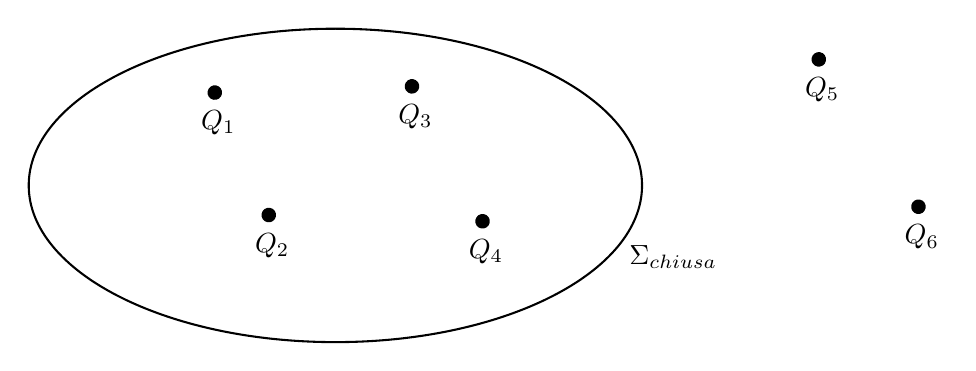
\begin{tikzpicture}[x=0.75pt,y=0.75pt,yscale=-1,xscale=1]
	%uncomment if require: \path (0,300); %set diagram left start at 0, and has height of 300

	%Shape: Ellipse [id:dp6166042155684706] 
	\draw   (100,109.5) .. controls (100,67.8) and (166.15,34) .. (247.75,34) .. controls (329.35,34) and (395.5,67.8) .. (395.5,109.5) .. controls (395.5,151.2) and (329.35,185) .. (247.75,185) .. controls (166.15,185) and (100,151.2) .. (100,109.5) -- cycle ;
	%Shape: Circle [id:dp4500030224947258] 
	\draw  [fill={rgb, 255:red, 0; green, 0; blue, 0 }  ,fill opacity=1 ] (187.14,63.15) .. controls (188.04,61.76) and (189.89,61.36) .. (191.29,62.25) .. controls (192.68,63.15) and (193.08,65.01) .. (192.18,66.4) .. controls (191.28,67.79) and (189.43,68.19) .. (188.03,67.3) .. controls (186.64,66.4) and (186.24,64.54) .. (187.14,63.15) -- cycle ;
	%Shape: Circle [id:dp9796248018777871] 
	\draw  [fill={rgb, 255:red, 0; green, 0; blue, 0 }  ,fill opacity=1 ] (282.14,60.15) .. controls (283.04,58.76) and (284.89,58.36) .. (286.29,59.25) .. controls (287.68,60.15) and (288.08,62.01) .. (287.18,63.4) .. controls (286.28,64.79) and (284.43,65.19) .. (283.03,64.3) .. controls (281.64,63.4) and (281.24,61.54) .. (282.14,60.15) -- cycle ;
	%Shape: Circle [id:dp09463099152199295] 
	\draw  [fill={rgb, 255:red, 0; green, 0; blue, 0 }  ,fill opacity=1 ] (213.14,122.15) .. controls (214.04,120.76) and (215.89,120.36) .. (217.29,121.25) .. controls (218.68,122.15) and (219.08,124.01) .. (218.18,125.4) .. controls (217.28,126.79) and (215.43,127.19) .. (214.03,126.3) .. controls (212.64,125.4) and (212.24,123.54) .. (213.14,122.15) -- cycle ;
	%Shape: Circle [id:dp33538641669305247] 
	\draw  [fill={rgb, 255:red, 0; green, 0; blue, 0 }  ,fill opacity=1 ] (316.14,125.15) .. controls (317.04,123.76) and (318.89,123.36) .. (320.29,124.25) .. controls (321.68,125.15) and (322.08,127.01) .. (321.18,128.4) .. controls (320.28,129.79) and (318.43,130.19) .. (317.03,129.3) .. controls (315.64,128.4) and (315.24,126.54) .. (316.14,125.15) -- cycle ;
	%Shape: Circle [id:dp8337517217710169] 
	\draw  [fill={rgb, 255:red, 0; green, 0; blue, 0 }  ,fill opacity=1 ] (478.14,47.15) .. controls (479.04,45.76) and (480.89,45.36) .. (482.29,46.25) .. controls (483.68,47.15) and (484.08,49.01) .. (483.18,50.4) .. controls (482.28,51.79) and (480.43,52.19) .. (479.03,51.3) .. controls (477.64,50.4) and (477.24,48.54) .. (478.14,47.15) -- cycle ;
	%Shape: Circle [id:dp4238901690042187] 
	\draw  [fill={rgb, 255:red, 0; green, 0; blue, 0 }  ,fill opacity=1 ] (526.14,118.15) .. controls (527.04,116.76) and (528.89,116.36) .. (530.29,117.25) .. controls (531.68,118.15) and (532.08,120.01) .. (531.18,121.4) .. controls (530.28,122.79) and (528.43,123.19) .. (527.03,122.3) .. controls (525.64,121.4) and (525.24,119.54) .. (526.14,118.15) -- cycle ;

	% Text Node
	\draw (191.33,79.42) node    {$Q_{1}$};
	% Text Node
	\draw (286.33,76.42) node    {$Q_{3}$};
	% Text Node
	\draw (217.33,138.42) node    {$Q_{2}$};
	% Text Node
	\draw (320.33,141.42) node    {$Q_{4}$};
	% Text Node
	\draw (482.33,63.42) node    {$Q_{5}$};
	% Text Node
	\draw (530.33,134.42) node    {$Q_{6}$};
	% Text Node
	\draw (410.5,144) node    {$\Sigma _{\text{chiusa}}$};

	\end{tikzpicture}
\end{figure}
\FloatBarrier

Se abbiamo un vero e proprio oggetto all'interno di $\Sigma$, dobbiamo andare a considerare la densità di carica di volume. E quindi:

\[
	Q_{\text{tot}}^{\text{interna a } \Sigma} = \int_{\tau}\rho d\tau
\]

\subsection{Applicazione del teorema di Gauss}

La legge di Gauss diventa uno strumento molto potente per determinare
il campo $\vec{E}$ nei casi in cui la distribuzione di carica che genera il campo presenti un elevato grado di \emph{simmetria} (sferica, cilindrica, piana). In queste condizioni di norma è facile individuare a priori l'andamento delle linee di forza e trovare di conseguenza delle superfici chiuse nei cui punti il campo è parallelo o ortogonale alla superficie stessa, per cui i contributi $\vec{E} \cdot \vec{n} \,dS$ o sono nulli o si scrivono facilmente.

\begin{figure}[htpb]
	\centering

	\tikzset{every picture/.style={line width=0.75pt}} %set default line width to 0.75pt        

	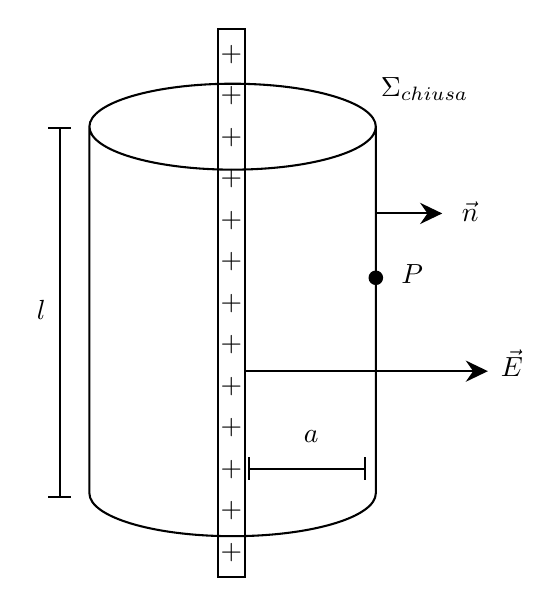
\begin{tikzpicture}[x=0.75pt,y=0.75pt,yscale=-1,xscale=1]
	%uncomment if require: \path (0,300); %set diagram left start at 0, and has height of 300

	%Shape: Rectangle [id:dp6271259438150636] 
	\draw   (230,11) -- (243,11) -- (243,275) -- (230,275) -- cycle ;
	%Straight Lines [id:da30089470945639274] 
	\draw    (243,176) -- (357,176) ;
	\draw [shift={(360,176)}, rotate = 180] [fill={rgb, 255:red, 0; green, 0; blue, 0 }  ][line width=0.08]  [draw opacity=0] (10.72,-5.15) -- (0,0) -- (10.72,5.15) -- (7.12,0) -- cycle    ;
	%Straight Lines [id:da9835619887853664] 
	\draw    (245,223) -- (301,223) ;
	\draw [shift={(301,223)}, rotate = 180] [color={rgb, 255:red, 0; green, 0; blue, 0 }  ][line width=0.75]    (0,5.59) -- (0,-5.59)   ;
	\draw [shift={(245,223)}, rotate = 180] [color={rgb, 255:red, 0; green, 0; blue, 0 }  ][line width=0.75]    (0,5.59) -- (0,-5.59)   ;
	%Shape: Circle [id:dp6971224069947288] 
	\draw  [fill={rgb, 255:red, 0; green, 0; blue, 0 }  ,fill opacity=1 ] (303,131) .. controls (303,129.34) and (304.34,128) .. (306,128) .. controls (307.66,128) and (309,129.34) .. (309,131) .. controls (309,132.66) and (307.66,134) .. (306,134) .. controls (304.34,134) and (303,132.66) .. (303,131) -- cycle ;
	%Straight Lines [id:da7901589292957081] 
	\draw    (153.67,236.5) -- (153.67,58.83) ;
	\draw [shift={(153.67,58.83)}, rotate = 450] [color={rgb, 255:red, 0; green, 0; blue, 0 }  ][line width=0.75]    (0,5.59) -- (0,-5.59)   ;
	\draw [shift={(153.67,236.5)}, rotate = 450] [color={rgb, 255:red, 0; green, 0; blue, 0 }  ][line width=0.75]    (0,5.59) -- (0,-5.59)   ;
	%Shape: Can [id:dp5914560994290878] 
	\draw   (306,58.2) -- (306,234.8) .. controls (306,246.23) and (275.11,255.5) .. (237,255.5) .. controls (198.89,255.5) and (168,246.23) .. (168,234.8) -- (168,58.2) .. controls (168,46.77) and (198.89,37.5) .. (237,37.5) .. controls (275.11,37.5) and (306,46.77) .. (306,58.2) .. controls (306,69.63) and (275.11,78.9) .. (237,78.9) .. controls (198.89,78.9) and (168,69.63) .. (168,58.2) ;
	%Straight Lines [id:da18093708742362602] 
	\draw    (306,100) -- (335,100) ;
	\draw [shift={(338,100)}, rotate = 180] [fill={rgb, 255:red, 0; green, 0; blue, 0 }  ][line width=0.08]  [draw opacity=0] (10.72,-5.15) -- (0,0) -- (10.72,5.15) -- (7.12,0) -- cycle    ;

	% Text Node
	\draw (236.4,23.4) node    {$+$};
	% Text Node
	\draw (236.4,43.4) node    {$+$};
	% Text Node
	\draw (236.4,63.4) node    {$+$};
	% Text Node
	\draw (236.4,83.4) node    {$+$};
	% Text Node
	\draw (236.4,103.4) node    {$+$};
	% Text Node
	\draw (236.4,123.4) node    {$+$};
	% Text Node
	\draw (236.4,143.4) node    {$+$};
	% Text Node
	\draw (236.4,163.4) node    {$+$};
	% Text Node
	\draw (236.4,183.4) node    {$+$};
	% Text Node
	\draw (236.4,203.4) node    {$+$};
	% Text Node
	\draw (236.4,223.4) node    {$+$};
	% Text Node
	\draw (236.4,243.4) node    {$+$};
	% Text Node
	\draw (236.4,263.4) node    {$+$};
	% Text Node
	\draw (323.5,129) node    {$P$};
	% Text Node
	\draw (274.83,207.33) node    {$a$};
	% Text Node
	\draw (144.83,146.67) node    {$l$};
	% Text Node
	\draw (371.5,172) node    {$\vec{E}$};
	% Text Node
	\draw (351.5,99) node    {$\vec{n}$};
	% Text Node
	\draw (329.5,40) node    {$\Sigma _{\text{chiusa}}$};

	\end{tikzpicture}
\end{figure}
\FloatBarrier

Consideriamo un filo rettilineo infinito carico con densità di carica lineare costante $\lambda$. Vogliamo determinare l'entità del campo elettrico in un certo punto $P$ ad una certa distanza. Il campo deve essere dotato di simmetria cilindrica. Significa che possiamo in generale scriverlo in tal modo:

\[
	\vec{E} (P) = E(a) \vec{n}
\]

Per applicare il teorema di Gauss dovremo immaginare una superficie astratta, che prende il nome di \textbf{superficie gaussiana}.
Consideriamo una superficie gaussiana che abbia la stessa simmetria cilindrica. Le due basi tuttavia non contribuiscono al flusso totale perché il prodotto scalare fra $\vec{E}$ e $\vec{n}$ sarà zero.

\[
	\Phi (\vec{E}) = \int_{\Sigma} \vec{E} \cdot \vec{n} dS = \Phi_{\text{base 1}} (\vec{E}) + \Phi_{\text{base 2}} (\vec{E}) + \Phi_{\text{sup. laterale}} (\vec{E})
\]

Il versore normale $\vec{n}$ coincide con $\vec{u}_r$ per tutti i punti della superficie laterale. Il primo risultato dell'aver scelto una superficie con la stessa simmetria del campo è che abbiamo semplificato la parte vettoriale. Stiamo calcolando questo integrale su una superficie cilindrica laterale che per definizione è il luogo dei punti equidistanti dal centro dall'asse, tutti alla distanza $a$. $\vec{E}(a)$ è costante, essendo funzione della posizione. Possiamo portare quindi il termine fuori dall'integrale.

\begin{align*}
	\Phi (\vec{E}) &= \int_{\text{sup. laterale}} E(a)\vec{u}_r \cdot \vec{n} dS \\
	\frac{Q_{\text{tot}}^{\Sigma}}{\varepsilon_0} &= E(a) \int_{\text{sup. laterale}} dS \tag*{T. di Gauss a primo membro} \\
	\frac{\int\lambda\,dl}{\varepsilon_0} &= E(a) \; 2\pi a\;l \\
	\frac{\lambda\,l}{\varepsilon_0} &= E(a) \; 2\pi a\;l \tag*{$\lambda$ è costante} \\
	E(a) &= \frac{\lambda}{2\pi a\varepsilon_0} \tag*{Campo elettrico generato da un filo} \\
\end{align*}

\section{I Equazione di Maxwell (anche in regime tempovariante)}

Si ricava a partire dal teorema di Gauss per il campo elettrico e dal teorema della Divergenza.
Data una superficie $\Sigma$ chiusa, di volume $\tau$ e densità di carica volumetrica $\rho (x,y,z)$ si ha

\[
	\Phi_{\Sigma}(\vec{E}) = \int_{\Sigma}\vec{E} \cdot \vec{n} dS = \frac{Q_{\text{tot}}^{\text{int}}}{\varepsilon_0}
\]

L'espressione della carica interna risulta essere

\[
	Q_{\text{tot}}^{\text{int}} = \int_{\tau} \rho (x,y,z)d\tau
\]

Sostituendola nell'espressione del flusso e applicando il teorema della divergenza si ottiene

\[
	\int_{\tau} \frac{\rho (x,y,z)}{\varepsilon_0}d\tau = \int_{\Sigma}\vec{E} \cdot \vec{n} dS = \int_{\tau} \text{div}\vec{E} \;d\tau
\]

Dal momento che gli integrali non dipendono né da $ \rho (x,y,z) $ né dalla forma della superficie, le funzioni integrande del primo e del terzo integrale devono essere uguali. Per cui

\[
	\boxed{\text{div}\vec{E} = \vec{\nabla} \cdot \vec{E} = \frac{\rho (x,y,z)}{\varepsilon_0}}
\]

Questa equazione ottenuta è detta anche \textbf{prima equazione di Maxwell} ed è in pratica la trasposizione in forma locale del teorema di Gauss. Essa ci dice che se in una regione dello spazio ho una densità di carica maggiore di zero, allora la divergenza è maggiore di zero. Significa che in quel punto c'è la sorgente positiva delle linee di flusso. Se abbiamo cariche negative varrà esattamente il contrario. Se $\rho$ è uguale a zero vale la proprietà sopra citata per il tubo di flusso.
Da questa equazione ricaviamo che:

\[
	\text{div}\vec{E} d\tau =\frac{\rho d\tau}{\varepsilon_0} = \frac{dq}{\varepsilon_0} = d\Phi (\vec{E}) \implies \text{div}\vec{E} = \frac{d\Phi (\vec{E})}{d\tau}
\]

\subsection{Calcolo della divergenza}

Esiste una formula pratica alternativa per calcolare la divergenza. Scegliamo un sistema di coordinate cartesiane per rappresentare il campo vettoriale.

\[
	\vec{v}(P) = v_x(x,y,z)\vec{u}_x + v_y(x,y,z)\vec{u}_y + v_z(x,y,z)\vec{u}_z
\]

Si può dimostrare che la divergenza del campo $\vec{v}$ è:

\[
	\text{div}\vec{v} = \frac{\partial v_x}{\partial x} + \frac{\partial v_y}{\partial y} + \frac{\partial v_z}{\partial z}
\]

Nel caso di altri sistemi di riferimento la formula può apparire molto più complicata. Ciascuno dei tre componenti dipende da tutte e tre le coordinate dello spazio.

\begin{figure}[htpb]
	\centering

	\tikzset{every picture/.style={line width=0.75pt}} %set default line width to 0.75pt        

	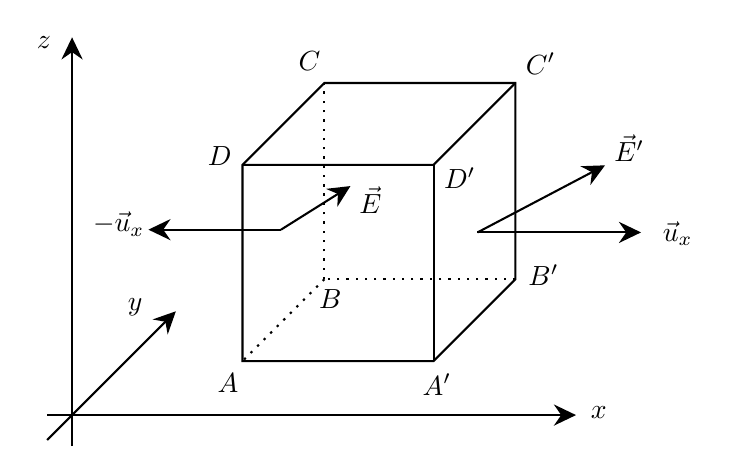
\begin{tikzpicture}[x=0.75pt,y=0.75pt,yscale=-1,xscale=1]
	%uncomment if require: \path (0,300); %set diagram left start at 0, and has height of 300

	%Straight Lines [id:da5013518463598057] 
	\draw    (130.88,228) -- (382.67,228) ;
	\draw [shift={(385.67,228)}, rotate = 180] [fill={rgb, 255:red, 0; green, 0; blue, 0 }  ][line width=0.08]  [draw opacity=0] (10.72,-5.15) -- (0,0) -- (10.72,5.15) -- (7.12,0) -- cycle    ;
	%Straight Lines [id:da6443750190887165] 
	\draw    (142.88,243) -- (142.88,49) ;
	\draw [shift={(142.88,46)}, rotate = 450] [fill={rgb, 255:red, 0; green, 0; blue, 0 }  ][line width=0.08]  [draw opacity=0] (10.72,-5.15) -- (0,0) -- (10.72,5.15) -- (7.12,0) -- cycle    ;
	%Straight Lines [id:da8305005539386254] 
	\draw    (130.88,240) -- (190.76,180.12) ;
	\draw [shift={(192.88,178)}, rotate = 495] [fill={rgb, 255:red, 0; green, 0; blue, 0 }  ][line width=0.08]  [draw opacity=0] (10.72,-5.15) -- (0,0) -- (10.72,5.15) -- (7.12,0) -- cycle    ;
	%Shape: Cube [id:dp6333624936608848] 
	\draw   (225,107.45) -- (264.45,68) -- (356.5,68) -- (356.5,162.55) -- (317.05,202) -- (225,202) -- cycle ; \draw   (356.5,68) -- (317.05,107.45) -- (225,107.45) ; \draw   (317.05,107.45) -- (317.05,202) ;
	%Straight Lines [id:da0547620432904663] 
	\draw  [dash pattern={on 0.84pt off 2.51pt}]  (264.45,162.55) -- (264.45,68) ;
	%Straight Lines [id:da7246817021460845] 
	\draw  [dash pattern={on 0.84pt off 2.51pt}]  (356.5,162.55) -- (264,162.55) ;
	%Straight Lines [id:da9803429259301326] 
	\draw  [dash pattern={on 0.84pt off 2.51pt}]  (264.45,162.55) -- (225.33,201.67) ;
	%Straight Lines [id:da5389134330495531] 
	\draw    (338.21,140) -- (414,140) ;
	\draw [shift={(417,140)}, rotate = 180] [fill={rgb, 255:red, 0; green, 0; blue, 0 }  ][line width=0.08]  [draw opacity=0] (10.72,-5.15) -- (0,0) -- (10.72,5.15) -- (7.12,0) -- cycle    ;
	%Straight Lines [id:da1347325077764896] 
	\draw    (338.21,140) -- (397.01,109.06) ;
	\draw [shift={(399.67,107.67)}, rotate = 512.25] [fill={rgb, 255:red, 0; green, 0; blue, 0 }  ][line width=0.08]  [draw opacity=0] (10.72,-5.15) -- (0,0) -- (10.72,5.15) -- (7.12,0) -- cycle    ;
	%Straight Lines [id:da48588431974198354] 
	\draw    (243.55,138.67) -- (182.67,138.67) ;
	\draw [shift={(179.67,138.67)}, rotate = 360] [fill={rgb, 255:red, 0; green, 0; blue, 0 }  ][line width=0.08]  [draw opacity=0] (10.72,-5.15) -- (0,0) -- (10.72,5.15) -- (7.12,0) -- cycle    ;
	%Straight Lines [id:da7358212844953658] 
	\draw    (243.55,138.67) -- (274.46,119.26) ;
	\draw [shift={(277,117.67)}, rotate = 507.88] [fill={rgb, 255:red, 0; green, 0; blue, 0 }  ][line width=0.08]  [draw opacity=0] (10.72,-5.15) -- (0,0) -- (10.72,5.15) -- (7.12,0) -- cycle    ;

	% Text Node
	\draw (396.67,226.67) node    {$x$};
	% Text Node
	\draw (129.33,48.67) node    {$z$};
	% Text Node
	\draw (173.33,176) node    {$y$};
	% Text Node
	\draw (218,212.67) node    {$A$};
	% Text Node
	\draw (318.67,213.33) node    {$A'$};
	% Text Node
	\draw (370,160.67) node    {$B'$};
	% Text Node
	\draw (267.33,172.33) node    {$B$};
	% Text Node
	\draw (214,103.33) node    {$D$};
	% Text Node
	\draw (257.33,57.33) node    {$C$};
	% Text Node
	\draw (368.67,58.67) node    {$C'$};
	% Text Node
	\draw (329.67,114) node    {$D'$};
	% Text Node
	\draw (434.67,140.67) node    {$\vec{u}_{x}$};
	% Text Node
	\draw (411.33,99.33) node    {$\vec{E} '$};
	% Text Node
	\draw (286.67,124.67) node    {$\vec{E}$};
	% Text Node
	\draw (165.33,136) node    {$-\vec{u}_{x}$};

	\end{tikzpicture}
\end{figure}
\FloatBarrier

\emph{Dimostrazione.} Consideriamo un parallelepipedo infinitesimo con gli spigoli $dx$, $dy$, $dz$ paralleli agli assi che che contiene la carica $dq=\rho(x,y,z) d\tau $, essendo $d\tau = dx\ dy\ dz$ il volume del parallelepipedo. Il flusso attraverso la superficie $A' B' C' D'$, perpendicolare all'asse $x$, è dato da:

\[
	\vec{E}' \vec{u}_x dydz = E_x'dydz
\]

Se indichiamo con $E_x'$ la componente di $\vec{E}'$ parallela all'asse $x$. Analogamente, il flusso attraverso la faccia $ABCD$ è:

\[
	\vec{E} (-\vec{u}_x)dydz = -E_x dydz
\]

Infatti la normale alla superficie orientata verso l'esterno è $-\vec{u}_x$ per la faccia $ABCD$. Complessivamente

\[
	(E_x'-E_x)dydz = \frac{\partial E_x}{\partial x} dx\,dy\,dz
\]
È il flusso attraverso le due superfici considerate. Espressioni simili si hanno per le altre coppie di superficie e quindi il flusso attraverso la superficie del parallelepipedo è:

\begin{align*}
	d\Phi &= \left( \frac{\partial E_x}{\partial x} +\frac{\partial E_y}{\partial y} + \frac{\partial E_z}{\partial z}  \right) dx\,dy\,dz \\
	&= \left( \frac{\partial E_x}{\partial x} +\frac{\partial E_y}{\partial y} + \frac{\partial E_z}{\partial z}  \right) d\tau
\end{align*}

Si ha che la divergenza del campo $\vec{E}$ è:

\[
	\boxed{\text{div}\vec{E} = \vec{\nabla} \cdot \vec{E} = \frac{d\Phi}{d\tau} = \frac{\partial E_x}{\partial x} + \frac{\partial E_y}{\partial y} + \frac{\partial E_z}{\partial z}}
\]

La divergenza del campo nel punto $P$ è data dal rapporto tra il flusso attraverso la superficie di un parallelepipedo infinitesimo centrato su $P$ e il volume del parallelepipedo.

\section{Conservatività del Campo Elettrico}

Come già affrontato in Fisica I, si dimostra che il lavoro compiuto dalla risultante delle forze agenti sull'oggetto, $\vec{R}$, è uguale alla variazione di energia cinetica dell'oggetto. In genere il lavoro dipende anche dal percorso scelto per andare da $A$ a $B$. Nel caso del teorema dell'energia cinetica, a parità di punti $A$ e $B$ e di velocità iniziale, a seconda del percorso che scelgo potrei avere la velocità finale diversa. Tuttavia talvolta possiamo lavorare con campi di forza di particolari proprietà.

Nel caso di forze conservative, qualunque sia la traiettoria seguita, la somma dei lavori compiuti è sempre la stessa, basta che siano fissati $A$ e $B$. Accade che allora possiamo esprimere il lavoro con un campo scalare che chiamiamo energia potenziale. Il lavoro di $\vec{R}$ lungo una traiettoria si può scrivere come la differenza fra l'energia potenziale nel punto di partenza e quella nel punto di arrivo. Lavoro ed energia si misurano in Joule.
Nel caso più generale in cui il nostro oggetto si muova in presenza sia di forze conservative che di forze non conservative, si dimostra un bilancio energetico molto importante. Definita energia meccanica dell'oggetto come la somma dell'energia cinetica $K$ e dell'energia potenziale $U$ del nostro oggetto, si dimostra che da $A$ a $B$ la variazione dell'energia meccanica è uguale al lavoro delle forze non conservative

\[
	\Delta E_{\text{mecc}} = E(B) - E(A) = \mathcal{L}_{NC}
\]

Se le forze non conservative sono nulle, allora vale il principio di conservazione dell'energia meccanica. Utilizzeremo questa proprietà quando ci occuperemo del moto di cariche elettriche.
Durante il moto delle particelle l'energia totale, somma dell'energia cinetica e dell'energia potenziale, rimane costante:

\[
	\Delta E_K + \Delta E_p = 0
\]

Dalla formula si vede chiaramente che scegliendo opportunamente il segno della differenza di potenziale è possibile accelerare la particella, trasformando l'energia potenziale in energia cinetica. Una carica positiva è accelerata se $V(A)>V(B)$ mentre una carica negativa è accelerata se $V(B)>V(A)$. Se $V(B)=V(A)$ non c'è alcun effetto complessivo; ciò non vuol dire che tra $A$ e $B$ non c'è campo, ma semplicemente che nel percorso $A\to B$ ci sono zone in cui l'effetto è accelerante e altre in cui è decelerante. In particolare $V(A)=V(B)$ se $A$ e $B$ coincidono. Alla fine di un percorso chiuso l'energia cinetica è la stessa che all'inizio, può essere cambiata in direzione, ma non di modulo.
Per le forze conservative vale anche un corollario. Se consideriamo un percorso $\Gamma$ in cui l'oggetto parte da $A$ e ritorna in $A$, allora in questo caso il lavoro compiuto dalla forza è zero.

\[
	\mathcal{L}_{AB}^{(FC)} = \oint_{\gamma} \vec{F}_cd\vec{l} = 0 = U(A) - U(A)
\]

Chiameremo l'integrale di linea su una linea chiusa \textbf{circuitazione}.

Sia una carica $Q$ fissa nello spazio ed una seconda carica esploratrice $q$ che si muove da un punto $A$ ad un punto $B$ sotto l'influenza di $Q$.

\begin{figure}[htpb]
	\centering

	\tikzset{every picture/.style={line width=0.75pt}} %set default line width to 0.75pt        

	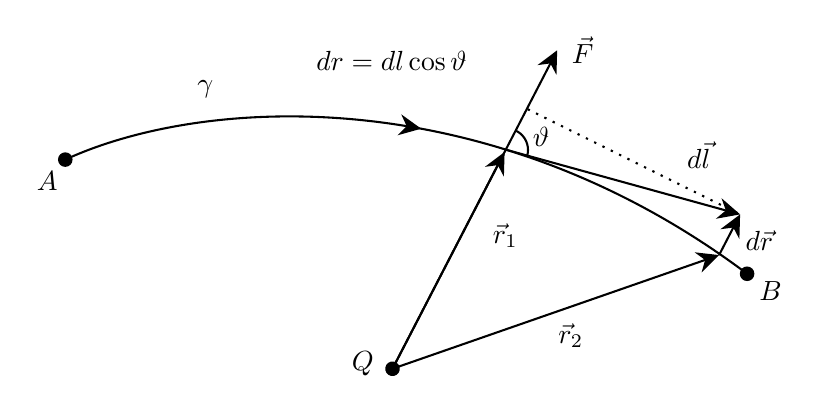
\begin{tikzpicture}[x=0.75pt,y=0.75pt,yscale=-1,xscale=1]
	%uncomment if require: \path (0,300); %set diagram left start at 0, and has height of 300

	%Curve Lines [id:da26092883666409095] 
	\draw    (80,106) .. controls (147.5,75) and (284.5,68) .. (408.5,161) ;
	\draw [shift={(251.49,91.11)}, rotate = 190.1] [fill={rgb, 255:red, 0; green, 0; blue, 0 }  ][line width=0.08]  [draw opacity=0] (10.72,-5.15) -- (0,0) -- (10.72,5.15) -- (7.12,0) -- cycle    ;
	%Shape: Circle [id:dp8590828188159274] 
	\draw  [fill={rgb, 255:red, 0; green, 0; blue, 0 }  ,fill opacity=1 ] (235.14,205.15) .. controls (236.04,203.76) and (237.89,203.36) .. (239.29,204.25) .. controls (240.68,205.15) and (241.08,207.01) .. (240.18,208.4) .. controls (239.28,209.79) and (237.43,210.19) .. (236.03,209.3) .. controls (234.64,208.4) and (234.24,206.54) .. (235.14,205.15) -- cycle ;
	%Straight Lines [id:da42137116431156296] 
	\draw    (237.66,206.77) -- (315.62,56) ;
	\draw [shift={(317,53.33)}, rotate = 477.34] [fill={rgb, 255:red, 0; green, 0; blue, 0 }  ][line width=0.08]  [draw opacity=0] (10.72,-5.15) -- (0,0) -- (10.72,5.15) -- (7.12,0) -- cycle    ;
	%Straight Lines [id:da9044377847250542] 
	\draw    (237.66,206.77) -- (290.29,104.99) ;
	\draw [shift={(291.67,102.33)}, rotate = 477.34] [fill={rgb, 255:red, 0; green, 0; blue, 0 }  ][line width=0.08]  [draw opacity=0] (10.72,-5.15) -- (0,0) -- (10.72,5.15) -- (7.12,0) -- cycle    ;
	%Straight Lines [id:da7481439852023828] 
	\draw    (237.66,206.77) -- (392.17,152.99) ;
	\draw [shift={(395,152)}, rotate = 520.81] [fill={rgb, 255:red, 0; green, 0; blue, 0 }  ][line width=0.08]  [draw opacity=0] (10.72,-5.15) -- (0,0) -- (10.72,5.15) -- (7.12,0) -- cycle    ;
	%Straight Lines [id:da34856183856557954] 
	\draw    (292.67,101.33) -- (402.24,131.6) ;
	\draw [shift={(405.13,132.4)}, rotate = 195.44] [fill={rgb, 255:red, 0; green, 0; blue, 0 }  ][line width=0.08]  [draw opacity=0] (10.72,-5.15) -- (0,0) -- (10.72,5.15) -- (7.12,0) -- cycle    ;
	%Shape: Boxed Line [id:dp6249319096386896] 
	\draw    (395,152) -- (403.76,135.06) ;
	\draw [shift={(405.13,132.4)}, rotate = 477.34] [fill={rgb, 255:red, 0; green, 0; blue, 0 }  ][line width=0.08]  [draw opacity=0] (10.72,-5.15) -- (0,0) -- (10.72,5.15) -- (7.12,0) -- cycle    ;
	%Straight Lines [id:da14116411953143926] 
	\draw  [dash pattern={on 0.84pt off 2.51pt}]  (302.8,81.73) -- (405.13,132.4) ;
	%Shape: Arc [id:dp31567400253761524] 
	\draw  [draw opacity=0] (296.84,91.94) .. controls (300.44,93.54) and (302.94,97.14) .. (302.94,101.33) .. controls (302.94,102.26) and (302.82,103.16) .. (302.58,104.01) -- (292.67,101.33) -- cycle ; \draw   (296.84,91.94) .. controls (300.44,93.54) and (302.94,97.14) .. (302.94,101.33) .. controls (302.94,102.26) and (302.82,103.16) .. (302.58,104.01) ;
	%Shape: Circle [id:dp4555289917735088] 
	\draw  [fill={rgb, 255:red, 0; green, 0; blue, 0 }  ,fill opacity=1 ] (77,106) .. controls (77,104.34) and (78.34,103) .. (80,103) .. controls (81.66,103) and (83,104.34) .. (83,106) .. controls (83,107.66) and (81.66,109) .. (80,109) .. controls (78.34,109) and (77,107.66) .. (77,106) -- cycle ;
	%Shape: Circle [id:dp09958237772920753] 
	\draw  [fill={rgb, 255:red, 0; green, 0; blue, 0 }  ,fill opacity=1 ] (405.5,161) .. controls (405.5,159.34) and (406.84,158) .. (408.5,158) .. controls (410.16,158) and (411.5,159.34) .. (411.5,161) .. controls (411.5,162.66) and (410.16,164) .. (408.5,164) .. controls (406.84,164) and (405.5,162.66) .. (405.5,161) -- cycle ;

	% Text Node
	\draw (223.33,204.42) node    {$Q$};
	% Text Node
	\draw (329.33,53.33) node    {$\vec{F}$};
	% Text Node
	\draw (292,142.67) node    {$\vec{r}_{1}$};
	% Text Node
	\draw (309.2,94.87) node    {$\vartheta $};
	% Text Node
	\draw (147.5,72.07) node    {$\gamma $};
	% Text Node
	\draw (323.6,190.67) node    {$\vec{r}_{2}$};
	% Text Node
	\draw (414.4,145.07) node    {$d\vec{r}$};
	% Text Node
	\draw (385.2,103.87) node    {$d\vec{l}$};
	% Text Node
	\draw (237.2,58.67) node    {$dr=dl\cos \vartheta $};
	% Text Node
	\draw (71.33,116.42) node    {$A$};
	% Text Node
	\draw (419.83,169.42) node    {$B$};

	\end{tikzpicture}
\end{figure}
\FloatBarrier

La forza agente sulla carica sarà repulsiva e sappiamo calcolarla grazie alla legge di Coulomb.
Calcoliamo il lavoro che $\vec{F}$ compie nello spostare $q$ da $A$ a $B$.

\begin{align*}
	\mathcal{L}_{AB,\gamma} = \int_{A,\gamma}^B \vec{F} \cdot d\vec{l} &= \int_A^B \frac{Qq\vec{u}_r\cdot d\vec{l}}{4\pi \varepsilon_0 r^2}   \tag*{$\vec{u}_r\cdot d\vec{l} = dl\,\cos \vartheta $} \\
	&= \int_A^B \frac{Qq\,dl\,\cos \vartheta}{4\pi \varepsilon_0 r^2} \tag*{$dl\,\cos \vartheta = dr $}\\
	&= \int_A^B \frac{Qq\,dr}{4\pi \varepsilon_0 r^2} \\
	&= \frac{Qq}{4\pi \varepsilon_0}\int_{r_A}^{r_B} \frac{dr}{r^2} \\
	&= \frac{Qq}{4\pi \varepsilon_0} \left[ -\frac{1}{r} \right]_{r_A}^{r_B} = \underbrace{\frac{Qq}{4\pi \varepsilon_0 r_A}}_{U(A)} - \underbrace{\frac{Qq}{4\pi \varepsilon_0 r_B}}_{U(B)}
\end{align*}

Vediamo che $\vec{F}$ è conservativa perché dipende solo dal punto di partenza e da quello di arrivo. L'energia potenziale elettrostatica sarà quindi data da:

\[
	\boxed{U_{\text{elettrostatica}} = \frac{Qq}{4\pi \varepsilon_0 r}}
\]

La convenzione è che l'energia potenziale sia nulla all'infinito ($U(\infty)=0$), tuttavia è pur sempre possibile definire l'energia potenziale elettrostatica a meno di una costante.
La forza coulombiana è una forza conservativa. Sappiamo che è possibile esprimere $\vec{F}$ se conosciamo il valore del campo elettrico nel punto occupato dalla carica esploratrice $ \vec{F} (P) = q\vec{E} (P) $. Possiamo sostituire questa uguaglianza nell'espressione del lavoro e otterremo che:

\begin{align*}
	\mathcal{L}_{AB} &= \int_A^B  \vec{F} \cdot d\vec{l}  = \int_A^B  q\vec{E} (P) \cdot d\vec{l} = q \int_A^B \vec{E} (P) \cdot d\vec{l} \\
	\frac{\mathcal{L}_{AB}}{q} &= \int_A^B \vec{E} (P) \cdot d\vec{l} \\
	\frac{U(A) - U(B)}{q}&= \int_A^B \vec{E} (P) \cdot d\vec{l} \\
	\underbrace{\frac{U(A)}{q}}_{V(A)} - \underbrace{\frac{U(B)}{q}}_{V(B)} &= \int_A^B \vec{E} (P) \cdot d\vec{l} \\
	V(A) - V(B) &= \int_A^B \vec{E} (P) \cdot d\vec{l} \\
	- \Delta V &= \int_A^B \vec{E} (P) \cdot d\vec{l}
\end{align*}

Chiamiamo l'espressione

\[
	\boxed{V(P) = \frac{U(P)}{q}}
\]
\textbf{potenziale elettrostatico} generato nel punto $P$ dalla carica sorgente $Q$. Avendo già definito l'energia potenziale elettrostatica, risulta che:

\[
	V(P) = \frac{U(P)}{q} = \frac{\frac{Qq}{4\pi \varepsilon_0 r}}{q} = \frac{Q}{4\pi \varepsilon_0 r}
\]

La dipendenza dalla carica esploratrice scompare. Anche l'energia potenziale è definita a meno di una costante ma ciò non ha rilevanza perché noi avremo sempre a che fare con delle differenze. Le dimensioni di questa nuova funzione introdotta sono quelle di una energia su una carica e dunque l'unità di misura sarebbe:

\[
	\frac{[E]}{[C]} = \left( \frac{J}{C} \right) = V \quad \text{Volt}
\]

Il potenziale ha una importanza notevole nella teoria dell'elettromagnetismo, quindi ribattezziamo questa unità di misura con un nome proprio, il Volt. Fissato il potenziale all'infinito pari a $0$, possiamo immaginare il potenziale in un punto $P$ come il lavoro che la forza elettrica compie per spostare una carica positiva unitaria da quel punto all'infinito.
L'integrale trovato

\[
	\boxed{\int_A^B \vec{E} \cdot d\vec{l} = V(A) - V(B)}
\]

dipende solo dai valori che la funzione $V(P)$ assume nel punto di partenza e di arrivo. Questa proprietà ci ricorda quella delle forze conservative. Tale considerazione ci permette di estendere il concetto di conservatività a qualunque campo vettoriale. Diciamo che \emph{un campo vettoriale è conservativo se l'integrale di linea in $d\vec{l}$ dipende solo dagli estremi e non dal percorso}. In questa accezione il campo elettrostatico è un campo conservativo. I campi elettrici non statici ma variabili nel tempo \emph{possono non essere conservativi}.

Tornando a considerare il lavoro compiuto dalla forza $\vec{F}$ per spostare $q$ da $A$ a $B$ una volta introdotto il potenziale elettrostatico, vediamo che esso si può anche riscrivere come:

\begin{gather*}
	\mathcal{L} = U(A) - U(B) = qV(A) - qV(B) = q[V(A)-V(B)] = -q\Delta V \\
	\boxed{\mathcal{L} = - q\Delta V}
\end{gather*}

Se vogliamo sapere il lavoro che le forze di Coulomb compiono per spostare la carica da $A$ a $B$, basta conoscere il potenziale elettrostatico in $A$ e in $B$. Ecco perché una delle unità di misura che ricorrono per il lavoro è l'\textbf{elettronvolt}, $eV$. Esso rappresenta l'energia acquisita da un elettrone quando si sposta di una differenza di potenziale di un Volt. Un elettronvolt è $1.6\times 10^{-19}$ Joule.
Un caso particolare è quello in cui eseguiamo una traiettoria chiusa in cui partendo dal punto $A$ torniamo ad $A$:

\[
	\oint_A \vec{E} \cdot d\vec{l} = V(A) - V(B) = 0 \quad \text{dato che} \quad V(A)=V(B)
\]

\begin{figure}[htpb]
	\centering

	\tikzset{every picture/.style={line width=0.75pt}} %set default line width to 0.75pt        

	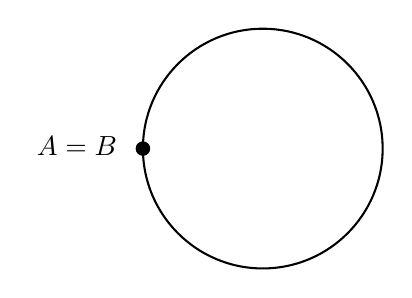
\begin{tikzpicture}[x=0.75pt,y=0.75pt,yscale=-1,xscale=1]
	%uncomment if require: \path (0,300); %set diagram left start at 0, and has height of 300

	%Shape: Circle [id:dp5572441369467569] 
	\draw   (207,110.75) .. controls (207,78.86) and (232.86,53) .. (264.75,53) .. controls (296.64,53) and (322.5,78.86) .. (322.5,110.75) .. controls (322.5,142.64) and (296.64,168.5) .. (264.75,168.5) .. controls (232.86,168.5) and (207,142.64) .. (207,110.75) -- cycle ;
	%Shape: Circle [id:dp7421877036925102] 
	\draw  [fill={rgb, 255:red, 0; green, 0; blue, 0 }  ,fill opacity=1 ] (204,110.75) .. controls (204,109.09) and (205.34,107.75) .. (207,107.75) .. controls (208.66,107.75) and (210,109.09) .. (210,110.75) .. controls (210,112.41) and (208.66,113.75) .. (207,113.75) .. controls (205.34,113.75) and (204,112.41) .. (204,110.75) -- cycle ;

	% Text Node
	\draw (175.2,109.4) node    {$A=B$};

	\end{tikzpicture}
\end{figure}
\FloatBarrier

Qualunque sia la linea chiusa, la circuitazione del campo elettrostatico è nulla. Ciò vale in generale nel caso di un campo conservativo. Se consideriamo una distribuzione di carica che genera questo campo elettrostatico, possiamo sempre immaginare che essa si possa scomporre in tante cariche puntiformi che eserciteranno sulla carica esploratrice una forza conservativa e quindi, ricordando che per le forze vale il principio di sovrapposizione degli effetti, \emph{la somma delle forze agenti sarà anch'essa conservativa}.
Ci sono diverse modalità per calcolare il potenziale elettrico in un punto.
Supponiamo di voler calcolare il potenziale di un punto particolare $P$ supponendo di conoscere il campo elettrico di qualsiasi punto dello spazio. Posso fissare il potenziale zero in un punto $P_0$, dal momento che è importante solo la differenza di potenziale. Avremo:

\[
	V(P) - \underbrace{V(P_0)}_{=0} = \int_{P_0}^P \vec{V} (P)d\vec{l} = V(P)
\]

Possiamo considerare anche più cariche puntiformi e sotto la loro influenza studiare il moto di una carica esploratrice $q$ da un punto $A$ a $B$. Per il principio di sovrapposizione degli effetti il campo elettrico totale in $P$ è la sommatoria del campi elettrici generati da ciascuna carica in $P$.

\begin{align*}
	V_{\text{tot}} (A) - V_{\text{tot}} (B) &= \int_A^B \vec{E}_{\text{tot}}d\vec{l} \\
	&= \int_A^B \left( \sum\nolimits_i \vec{E}_i   \right) \cdot  d\vec{l} \\
	&= \sum\nolimits_i \int_A^B \vec{E}_i\cdot d\vec{l} \\
	&= \sum\nolimits_i \left[ V(A)_i - V(B)_i   \right]
\end{align*}

Il potenziale totale generato da questa distribuzione di carica è la somma dei potenziali generati da ciascuna delle cariche presenti. Questo comporta che \emph{anche per il potenziale elettrostatico vale il principio della sovrapposizione degli effetti}. Possiamo allora estendere il ragionamento a una distribuzione di carica qualsiasi.

\begin{itemize}
	\item \emph{Potenziale generato da un volume} $\rho (x',y',z') $ \\
	Consideriamo ora un cubetto di volume $d\tau$ e carica $dq$ centrato in $P'(x',y',z')$. Sia $\vec{r}'$ variabile e $\vec{r}$ costante. Esprimiamo la carica $ dq = \rho (x',y',z') d\tau  $ e il potenziale infinitesimo $ dV = \frac{dq (\vec{r} -\vec{r}_i )}{4\pi \varepsilon_0 |\vec{r} -\vec{r}_i |^2} $ generato dalla distribuzione di carica nel punto $P$. Allora
	\begin{align*}
		V (P) = \int_{\text{oggetto}} dV &= \int_{\text{ogg.}} \frac{dq (\vec{r} -\vec{r}_i )}{4\pi \varepsilon_0 |\vec{r} -\vec{r}_i |^2}\\
		V (P) &= \int_{\tau} \frac{\rho (x',y',z') d\tau (\vec{r} -\vec{r}_i )}{4\pi \varepsilon_0 |\vec{r} -\vec{r}_i |^2} \\
		V (P) &= \int_{\tau} \frac{\rho (x',y',z') (\vec{r} -\vec{r}_i )}{4\pi \varepsilon_0 |\vec{r} -\vec{r}_i |^2}d\tau
	\end{align*}
	\begin{figure}[htpb]
		\centering
		

		\tikzset{every picture/.style={line width=0.75pt}} %set default line width to 0.75pt        

		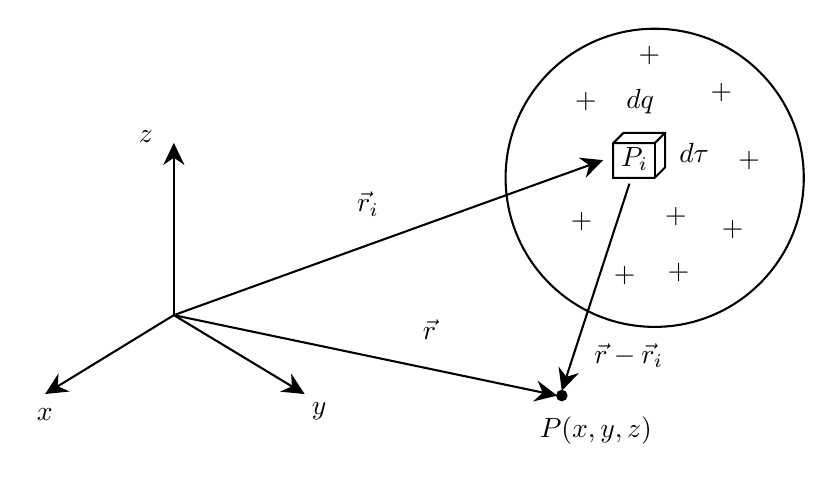
\begin{tikzpicture}[x=0.75pt,y=0.75pt,yscale=-1,xscale=1]
		%uncomment if require: \path (0,300); %set diagram left start at 0, and has height of 300

		%Straight Lines [id:da1780203758056127] 
		\draw    (185.5,165.67) -- (185.5,85.67) ;
		\draw [shift={(185.5,82.67)}, rotate = 450] [fill={rgb, 255:red, 0; green, 0; blue, 0 }  ][line width=0.08]  [draw opacity=0] (10.72,-5.15) -- (0,0) -- (10.72,5.15) -- (7.12,0) -- cycle    ;
		%Straight Lines [id:da633348072374383] 
		\draw    (185.5,165.67) -- (245.93,202.12) ;
		\draw [shift={(248.5,203.67)}, rotate = 211.1] [fill={rgb, 255:red, 0; green, 0; blue, 0 }  ][line width=0.08]  [draw opacity=0] (10.72,-5.15) -- (0,0) -- (10.72,5.15) -- (7.12,0) -- cycle    ;
		%Straight Lines [id:da5798881183189684] 
		\draw    (185.5,165.67) -- (126.06,202.1) ;
		\draw [shift={(123.5,203.67)}, rotate = 328.5] [fill={rgb, 255:red, 0; green, 0; blue, 0 }  ][line width=0.08]  [draw opacity=0] (10.72,-5.15) -- (0,0) -- (10.72,5.15) -- (7.12,0) -- cycle    ;
		%Shape: Circle [id:dp3554852517874745] 
		\draw  [fill={rgb, 255:red, 0; green, 0; blue, 0 }  ,fill opacity=1 ] (370.17,204.42) .. controls (370.17,203.17) and (371.17,202.17) .. (372.42,202.17) .. controls (373.66,202.17) and (374.67,203.17) .. (374.67,204.42) .. controls (374.67,205.66) and (373.66,206.67) .. (372.42,206.67) .. controls (371.17,206.67) and (370.17,205.66) .. (370.17,204.42) -- cycle ;
		%Straight Lines [id:da32003343045753363] 
		\draw    (185.5,165.67) -- (389.51,92.02) ;
		\draw [shift={(392.33,91)}, rotate = 520.15] [fill={rgb, 255:red, 0; green, 0; blue, 0 }  ][line width=0.08]  [draw opacity=0] (10.72,-5.15) -- (0,0) -- (10.72,5.15) -- (7.12,0) -- cycle    ;
		%Straight Lines [id:da11503891049993031] 
		\draw    (185.5,165.67) -- (367.23,203.8) ;
		\draw [shift={(370.17,204.42)}, rotate = 191.85] [fill={rgb, 255:red, 0; green, 0; blue, 0 }  ][line width=0.08]  [draw opacity=0] (10.72,-5.15) -- (0,0) -- (10.72,5.15) -- (7.12,0) -- cycle    ;
		%Straight Lines [id:da044847521882755315] 
		\draw    (405,102.33) -- (373.35,199.31) ;
		\draw [shift={(372.42,202.17)}, rotate = 288.08] [fill={rgb, 255:red, 0; green, 0; blue, 0 }  ][line width=0.08]  [draw opacity=0] (10.72,-5.15) -- (0,0) -- (10.72,5.15) -- (7.12,0) -- cycle    ;
		%Shape: Circle [id:dp39528053403956975] 
		\draw   (345.33,99.5) .. controls (345.33,59.83) and (377.49,27.67) .. (417.17,27.67) .. controls (456.84,27.67) and (489,59.83) .. (489,99.5) .. controls (489,139.17) and (456.84,171.33) .. (417.17,171.33) .. controls (377.49,171.33) and (345.33,139.17) .. (345.33,99.5) -- cycle ;
		%Shape: Cube [id:dp9932780936605101] 
		\draw   (397.17,82.83) -- (402.17,77.83) -- (422.17,77.83) -- (422.17,94.5) -- (417.17,99.5) -- (397.17,99.5) -- cycle ; \draw   (422.17,77.83) -- (417.17,82.83) -- (397.17,82.83) ; \draw   (417.17,82.83) -- (417.17,99.5) ;

		% Text Node
		\draw (123.33,213.67) node    {$x$};
		% Text Node
		\draw (255.5,212.17) node    {$y$};
		% Text Node
		\draw (172,79.67) node    {$z$};
		% Text Node
		\draw (404.67,185) node    {$\vec{r} -\vec{r}_{i}$};
		% Text Node
		\draw (308.67,172.83) node    {$\vec{r}$};
		% Text Node
		\draw (279,112.17) node    {$\vec{r}_{i}$};
		% Text Node
		\draw (410.17,63) node    {$dq$};
		% Text Node
		\draw (388.83,221.33) node    {$P( x ,y,z)$};
		% Text Node
		\draw (414.67,40.67) node    {$+$};
		% Text Node
		\draw (449.33,58.67) node    {$+$};
		% Text Node
		\draw (462.67,91.33) node    {$+$};
		% Text Node
		\draw (454.67,124.67) node    {$+$};
		% Text Node
		\draw (428.67,145.33) node    {$+$};
		% Text Node
		\draw (402.67,146.67) node    {$+$};
		% Text Node
		\draw (382,120.67) node    {$+$};
		% Text Node
		\draw (384,62.67) node    {$+$};
		% Text Node
		\draw (427.33,118) node    {$+$};
		% Text Node
		\draw (407.5,90.33) node    {$P_{i}$};
		% Text Node
		\draw (436.17,87.67) node    {$d\tau $};

		\end{tikzpicture}
	\end{figure}
	\FloatBarrier

	\item \emph{Potenziale generato da una superfie} $\sigma (x',y',z') $ \\
	Consideriamo ora una superficie infinitesima $dS$ e carica $dq$ in $P'(x',y',z')$. Sia $\vec{r}'$ variabile e $\vec{r}$ costante. Esprimiamo la carica $ dq = \sigma(x',y',z') dS $ e il potenziale infinitesimo $ dV = \frac{dq (\vec{r} -\vec{r}_i )}{4\pi \varepsilon_0 |\vec{r} -\vec{r}_i |^2} $ generato dalla distribuzione di carica nel punto $P$. Allora
	\begin{align*}
		V (P) &= \int_{\Sigma} \frac{\sigma  (x',y',z') (\vec{r} -\vec{r}_i )}{4\pi \varepsilon_0 |\vec{r} -\vec{r}_i |^2}dS
	\end{align*}
	\begin{figure}[htpb]
		\centering
		

		\tikzset{every picture/.style={line width=0.75pt}} %set default line width to 0.75pt        

		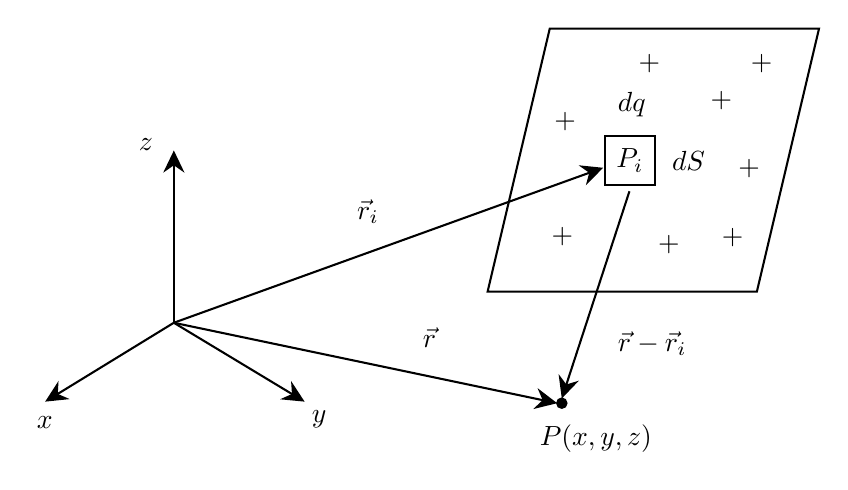
\begin{tikzpicture}[x=0.75pt,y=0.75pt,yscale=-1,xscale=1]
		%uncomment if require: \path (0,300); %set diagram left start at 0, and has height of 300

		%Straight Lines [id:da8132437964757075] 
		\draw    (173.5,185.67) -- (173.5,105.67) ;
		\draw [shift={(173.5,102.67)}, rotate = 450] [fill={rgb, 255:red, 0; green, 0; blue, 0 }  ][line width=0.08]  [draw opacity=0] (10.72,-5.15) -- (0,0) -- (10.72,5.15) -- (7.12,0) -- cycle    ;
		%Straight Lines [id:da3778404924799825] 
		\draw    (173.5,185.67) -- (233.93,222.12) ;
		\draw [shift={(236.5,223.67)}, rotate = 211.1] [fill={rgb, 255:red, 0; green, 0; blue, 0 }  ][line width=0.08]  [draw opacity=0] (10.72,-5.15) -- (0,0) -- (10.72,5.15) -- (7.12,0) -- cycle    ;
		%Straight Lines [id:da6935075526188754] 
		\draw    (173.5,185.67) -- (114.06,222.1) ;
		\draw [shift={(111.5,223.67)}, rotate = 328.5] [fill={rgb, 255:red, 0; green, 0; blue, 0 }  ][line width=0.08]  [draw opacity=0] (10.72,-5.15) -- (0,0) -- (10.72,5.15) -- (7.12,0) -- cycle    ;
		%Shape: Circle [id:dp9243675757036502] 
		\draw  [fill={rgb, 255:red, 0; green, 0; blue, 0 }  ,fill opacity=1 ] (358.17,224.42) .. controls (358.17,223.17) and (359.17,222.17) .. (360.42,222.17) .. controls (361.66,222.17) and (362.67,223.17) .. (362.67,224.42) .. controls (362.67,225.66) and (361.66,226.67) .. (360.42,226.67) .. controls (359.17,226.67) and (358.17,225.66) .. (358.17,224.42) -- cycle ;
		%Straight Lines [id:da37428712983736157] 
		\draw    (173.5,185.67) -- (377.51,112.02) ;
		\draw [shift={(380.33,111)}, rotate = 520.15] [fill={rgb, 255:red, 0; green, 0; blue, 0 }  ][line width=0.08]  [draw opacity=0] (10.72,-5.15) -- (0,0) -- (10.72,5.15) -- (7.12,0) -- cycle    ;
		%Straight Lines [id:da0777129682659603] 
		\draw    (173.5,185.67) -- (355.23,223.8) ;
		\draw [shift={(358.17,224.42)}, rotate = 191.85] [fill={rgb, 255:red, 0; green, 0; blue, 0 }  ][line width=0.08]  [draw opacity=0] (10.72,-5.15) -- (0,0) -- (10.72,5.15) -- (7.12,0) -- cycle    ;
		%Straight Lines [id:da4139198240649695] 
		\draw    (393,122.33) -- (361.35,219.31) ;
		\draw [shift={(360.42,222.17)}, rotate = 288.08] [fill={rgb, 255:red, 0; green, 0; blue, 0 }  ][line width=0.08]  [draw opacity=0] (10.72,-5.15) -- (0,0) -- (10.72,5.15) -- (7.12,0) -- cycle    ;
		%Flowchart: Data [id:dp9333451488015583] 
		\draw   (354.6,44) -- (484.33,44) -- (454.4,170.67) -- (324.67,170.67) -- cycle ;
		%Shape: Square [id:dp008818926916588365] 
		\draw   (381.17,95.5) -- (405.17,95.5) -- (405.17,119.5) -- (381.17,119.5) -- cycle ;

		% Text Node
		\draw (111.33,233.67) node    {$x$};
		% Text Node
		\draw (243.5,232.17) node    {$y$};
		% Text Node
		\draw (160,99.67) node    {$z$};
		% Text Node
		\draw (404,195.67) node    {$\vec{r} -\vec{r}_{i}$};
		% Text Node
		\draw (296.67,192.83) node    {$\vec{r}$};
		% Text Node
		\draw (267,132.17) node    {$\vec{r}_{i}$};
		% Text Node
		\draw (394.17,80.33) node    {$dq$};
		% Text Node
		\draw (376.83,241.33) node    {$P( x ,y,z)$};
		% Text Node
		\draw (402.67,60.67) node    {$+$};
		% Text Node
		\draw (437.33,78.67) node    {$+$};
		% Text Node
		\draw (450.67,111.33) node    {$+$};
		% Text Node
		\draw (442.67,144.67) node    {$+$};
		% Text Node
		\draw (456.67,60.67) node    {$+$};
		% Text Node
		\draw (360.67,144) node    {$+$};
		% Text Node
		\draw (362,88.67) node    {$+$};
		% Text Node
		\draw (412,148) node    {$+$};
		% Text Node
		\draw (393.17,107.5) node    {$P_{i}$};
		% Text Node
		\draw (421.5,107.67) node    {$dS$};

		\end{tikzpicture}
	\end{figure}
	\FloatBarrier

	\item \emph{Potenziale generato da una linea} $\lambda (x',y',z') $ \\
	Consideriamo ora un segmento infinitesimo $ dl   $ e carica $ dq $ in $ P'(x',y',z') $. Sia $ \vec{r}' $ variabile e $ \vec{r}  $ costante. Esprimiamo la carica $ dq = \lambda(x',y',z') dl $ e il potenziale infinitesimo $ dV = \frac{dq (\vec{r} -\vec{r}_i )}{4\pi \varepsilon_0 |\vec{r} -\vec{r}_i |^2} $ generato dalla distribuzione di carica nel punto $P$. Allora
	\begin{align*}
		V (P) &= \int_{\Lambda} \frac{\lambda  (x',y',z') (\vec{r} -\vec{r}_i )}{4\pi \varepsilon_0 |\vec{r} -\vec{r}_i |^2}dl
	\end{align*}
	\begin{figure}[htpb]
		\centering
		

		\tikzset{every picture/.style={line width=0.75pt}} %set default line width to 0.75pt        

		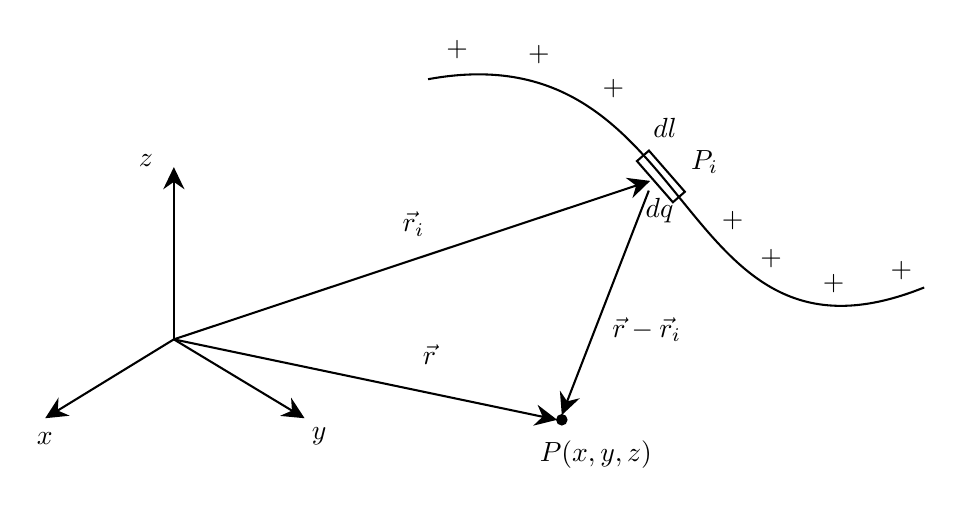
\begin{tikzpicture}[x=0.75pt,y=0.75pt,yscale=-1,xscale=1]
		%uncomment if require: \path (0,300); %set diagram left start at 0, and has height of 300

		%Straight Lines [id:da3248192246494668] 
		\draw    (168.5,188.67) -- (168.5,108.67) ;
		\draw [shift={(168.5,105.67)}, rotate = 450] [fill={rgb, 255:red, 0; green, 0; blue, 0 }  ][line width=0.08]  [draw opacity=0] (10.72,-5.15) -- (0,0) -- (10.72,5.15) -- (7.12,0) -- cycle    ;
		%Straight Lines [id:da20698176796558965] 
		\draw    (168.5,188.67) -- (228.93,225.12) ;
		\draw [shift={(231.5,226.67)}, rotate = 211.1] [fill={rgb, 255:red, 0; green, 0; blue, 0 }  ][line width=0.08]  [draw opacity=0] (10.72,-5.15) -- (0,0) -- (10.72,5.15) -- (7.12,0) -- cycle    ;
		%Straight Lines [id:da24095408360246595] 
		\draw    (168.5,188.67) -- (109.06,225.1) ;
		\draw [shift={(106.5,226.67)}, rotate = 328.5] [fill={rgb, 255:red, 0; green, 0; blue, 0 }  ][line width=0.08]  [draw opacity=0] (10.72,-5.15) -- (0,0) -- (10.72,5.15) -- (7.12,0) -- cycle    ;
		%Shape: Circle [id:dp8211498090043992] 
		\draw  [fill={rgb, 255:red, 0; green, 0; blue, 0 }  ,fill opacity=1 ] (353.17,227.42) .. controls (353.17,226.17) and (354.17,225.17) .. (355.42,225.17) .. controls (356.66,225.17) and (357.67,226.17) .. (357.67,227.42) .. controls (357.67,228.66) and (356.66,229.67) .. (355.42,229.67) .. controls (354.17,229.67) and (353.17,228.66) .. (353.17,227.42) -- cycle ;
		%Straight Lines [id:da4729626879808948] 
		\draw    (168.5,188.67) -- (395.15,113.28) ;
		\draw [shift={(398,112.33)}, rotate = 521.6] [fill={rgb, 255:red, 0; green, 0; blue, 0 }  ][line width=0.08]  [draw opacity=0] (10.72,-5.15) -- (0,0) -- (10.72,5.15) -- (7.12,0) -- cycle    ;
		%Straight Lines [id:da23097223788931975] 
		\draw    (168.5,188.67) -- (350.23,226.8) ;
		\draw [shift={(353.17,227.42)}, rotate = 191.85] [fill={rgb, 255:red, 0; green, 0; blue, 0 }  ][line width=0.08]  [draw opacity=0] (10.72,-5.15) -- (0,0) -- (10.72,5.15) -- (7.12,0) -- cycle    ;
		%Straight Lines [id:da9822371868780124] 
		\draw    (397.33,117) -- (356.5,222.37) ;
		\draw [shift={(355.42,225.17)}, rotate = 291.18] [fill={rgb, 255:red, 0; green, 0; blue, 0 }  ][line width=0.08]  [draw opacity=0] (10.72,-5.15) -- (0,0) -- (10.72,5.15) -- (7.12,0) -- cycle    ;
		%Curve Lines [id:da15270005504887885] 
		\draw    (291,63.33) .. controls (423.33,39) and (407.33,213) .. (530,163.67) ;
		%Shape: Rectangle [id:dp02403770120059212] 
		\draw   (397.4,97.73) -- (414.71,117.57) -- (408.94,122.61) -- (391.62,102.77) -- cycle ;

		% Text Node
		\draw (106.33,236.67) node    {$x$};
		% Text Node
		\draw (238.5,235.17) node    {$y$};
		% Text Node
		\draw (155,102.67) node    {$z$};
		% Text Node
		\draw (396.33,184) node    {$\vec{r} -\vec{r}_{i}$};
		% Text Node
		\draw (291.67,195.83) node    {$\vec{r}$};
		% Text Node
		\draw (284,133.17) node    {$\vec{r}_{i}$};
		% Text Node
		\draw (402.5,126.67) node    {$dq$};
		% Text Node
		\draw (371.83,244.33) node    {$P( x ,y,z)$};
		% Text Node
		\draw (305,49) node    {$+$};
		% Text Node
		\draw (380.33,67.67) node    {$+$};
		% Text Node
		\draw (456.33,149.67) node    {$+$};
		% Text Node
		\draw (486.33,161.67) node    {$+$};
		% Text Node
		\draw (344.33,51.67) node    {$+$};
		% Text Node
		\draw (519,155.67) node    {$+$};
		% Text Node
		\draw (424.17,103.17) node    {$P_{i}$};
		% Text Node
		\draw (405.17,86.67) node    {$dl$};
		% Text Node
		\draw (437.67,131.67) node    {$+$};

		\end{tikzpicture}
	\end{figure}
	\FloatBarrier

\end{itemize}

Consideriamo il caso di una carica che si sposta da $A$ a $B$ in un campo di forze conservative. L'energia meccanica totale sarà costante lungo la traiettoria. Avendo introdotto il potenziale, l'energia potenziale si può scrivere come il prodotto della carica $q$ per il potenziale generato da $Q$ in $P$. $ \Delta E = 0 \implies E(A)=E(B) $.
Le cariche elettriche se si muovono di moto accelerato emettono onde. Dunque il principio di conservazione dell'energia meccanica va preso con le pinze. Se la carica si muove lentamente la perdita di energia per irraggiamento è trascurabile. Se invece la particella accelera considerevolmente, è come se si muovesse in un fluido viscoso in cui viene rallentata perdendo energia sottoforma di onde elettromagnetiche. Nella meccanica relativistica questo fenomeno accade. Pertanto il principio di conservazione dell'energia meccanica ha dei limiti. Un fenomeno di questo tipo è osservabile anche nel mondo macroscopico: infatti le grandi masse quando accelerano emettono onde gravitazionali che portano via energia. Tuttavia è un energia molto più piccola rispetto a quella che porta via l'irraggiamento di onde elettromagnetiche.

\section{Energia elettrostatica}

L'energia elettrostatica di una distribuzione di carica è il lavoro che qualche forza esterna ha dovuto spendere per creare tale distribuzione. Cominciamo con il considerare una prima carica puntiforme $q_1$ dello spazio. Poniamo di voler portare in un punto $B$ una certa carica $q_2$ lungo un qualunque percorso. Chiamiamo la distanza fra le cariche $r_{12} $. Mentre portiamo $q_2$ dall'infinito a $B$, le cariche si respingono. Avremo una forza di repulsione da vincere per avvicinarle. Dovremo opporre alla forza di repulsione una forza esterna che la bilanci esattamente punto per punto.

\begin{figure}[htpb]
	\centering

	\tikzset{every picture/.style={line width=0.75pt}} %set default line width to 0.75pt        

	\begin{tikzpicture}[x=0.75pt,y=0.75pt,yscale=-1,xscale=1]
	%uncomment if require: \path (0,300); %set diagram left start at 0, and has height of 300

	%Curve Lines [id:da2598890702736305] 
	\draw    (270,123) .. controls (372.5,37) and (410.5,213) .. (515.5,134) ;
	\draw [shift={(392.88,126.58)}, rotate = 33.35] [fill={rgb, 255:red, 0; green, 0; blue, 0 }  ][line width=0.08]  [draw opacity=0] (10.72,-5.15) -- (0,0) -- (10.72,5.15) -- (7.12,0) -- cycle    ;
	%Shape: Circle [id:dp5297886834493957] 
	\draw  [fill={rgb, 255:red, 0; green, 0; blue, 0 }  ,fill opacity=1 ] (218.14,80.15) .. controls (219.04,78.76) and (220.89,78.36) .. (222.29,79.25) .. controls (223.68,80.15) and (224.08,82.01) .. (223.18,83.4) .. controls (222.28,84.79) and (220.43,85.19) .. (219.03,84.3) .. controls (217.64,83.4) and (217.24,81.54) .. (218.14,80.15) -- cycle ;
	%Shape: Circle [id:dp5663783446802324] 
	\draw  [fill={rgb, 255:red, 0; green, 0; blue, 0 }  ,fill opacity=1 ] (371.98,114.12) .. controls (372.88,112.73) and (374.73,112.33) .. (376.13,113.23) .. controls (377.52,114.13) and (377.92,115.98) .. (377.02,117.38) .. controls (376.12,118.77) and (374.27,119.17) .. (372.87,118.27) .. controls (371.48,117.37) and (371.08,115.52) .. (371.98,114.12) -- cycle ;
	%Straight Lines [id:da4768868780179971] 
	\draw    (374.5,115.75) -- (368.83,63.98) ;
	\draw [shift={(368.5,61)}, rotate = 443.75] [fill={rgb, 255:red, 0; green, 0; blue, 0 }  ][line width=0.08]  [draw opacity=0] (10.72,-5.15) -- (0,0) -- (10.72,5.15) -- (7.12,0) -- cycle    ;
	%Shape: Circle [id:dp8854072211352453] 
	\draw  [fill={rgb, 255:red, 0; green, 0; blue, 0 }  ,fill opacity=1 ] (199.14,176.15) .. controls (200.04,174.76) and (201.89,174.36) .. (203.29,175.25) .. controls (204.68,176.15) and (205.08,178.01) .. (204.18,179.4) .. controls (203.28,180.79) and (201.43,181.19) .. (200.03,180.3) .. controls (198.64,179.4) and (198.24,177.54) .. (199.14,176.15) -- cycle ;
	%Straight Lines [id:da10607471226633058] 
	\draw    (380.17,167.52) -- (374.5,115.75) ;
	\draw [shift={(380.5,170.5)}, rotate = 263.75] [fill={rgb, 255:red, 0; green, 0; blue, 0 }  ][line width=0.08]  [draw opacity=0] (10.72,-5.15) -- (0,0) -- (10.72,5.15) -- (7.12,0) -- cycle    ;

	% Text Node
	\draw (206.33,79.42) node    {$q_{2}$};
	% Text Node
	\draw (389.33,102.92) node    {$q_{3}$};
	% Text Node
	\draw (209.83,193.92) node    {$B$};
	% Text Node
	\draw (539.33,118.42) node    {$A( \infty )$};
	% Text Node
	\draw (187.33,175.42) node    {$q_{1}$};
	% Text Node
	\draw (276.83,135.92) node    {$C$};
	% Text Node
	\draw (389.33,62.92) node    {$\vec{F}_{c}$};
	% Text Node
	\draw (401.33,174.92) node    {$\vec{F}_{est}$};

	\end{tikzpicture}
\end{figure}
\FloatBarrier

Cerchiamo di capire qual è il lavoro che la forza esterna deve compiere per portare $q_2$ in $B$. Per calcolarlo sappiamo che:

\begin{align*}
	\mathcal{L} = \int_A^B \vec{F}_{\text{esterna}} \cdot d\vec{l} &= - \int_A^B \vec{F}_{\text{Coulomb}} \cdot d\vec{l} \\
	&= - [ q_2 \underbrace{V_1(A)}_{=0} - q_2V_1(B) ] \\
	&= q_2 V_1(B) = q_2 \, \frac{q_1}{4\pi \varepsilon_0 r_{12}} = U_e
\end{align*}

Chiameremo questa quantità \textbf{energia elettrostatica della distribuzione di cariche}. Se metto insieme delle cariche immagazzino in esse dell'energia e quando queste vengono liberate essa viene restituita. La distribuzione di carica è come un accumulatore di energia.
Se consideriamo la possibilità di avvicinare al sistema una terza carica $q_3$, quello che succederà è che il lavoro delle forze esterne per portare un'altra carica da $A$ a $C$ sarà uguale a:

\[
	\mathcal{L}_{AC}^{F_{\text{est}}}  = q_3 V_1(C) + q_3V_2(C) = \frac{q_3q_1}{4\pi \varepsilon_0 r_{31}} + \frac{q_3q_2}{4\pi \varepsilon_0 r_{32}}
\]

Questo è un lavoro aggiuntivo che si somma a quello compiuto prima per avvicinare le cariche. L'energia elettrostatica sarà la somma del lavoro per avvicinare tutte e tre le cariche.
In generale si ha:

\[
	\boxed{U_e = \frac{1}{2} \sum_{i\neq j} \frac{q_iq_j}{4\pi \varepsilon_0 r_{ij}}}
\]

Siccome $r_{ij} = r_{ji}$, risulta evidente che ogni contributo compare due volte e pertanto il risultato è quello sopra.

\section{Il campo come gradiente del potenziale}

Immaginiamo due punti $A$ e $B$ molto vicini fra loro, separati da uno spostamento infinitesimo $d\vec{l}$. Supponiamo che in tale regione ci sia un campo elettrico.

\begin{figure}[htpb]
	\centering

	\tikzset{every picture/.style={line width=0.75pt}} %set default line width to 0.75pt        

	\begin{tikzpicture}[x=0.75pt,y=0.75pt,yscale=-1,xscale=1]
	%uncomment if require: \path (0,300); %set diagram left start at 0, and has height of 300

	%Straight Lines [id:da3608378869469364] 
	\draw    (395.72,126.13) -- (223.66,195.77) ;
	\draw [shift={(398.5,125)}, rotate = 157.96] [fill={rgb, 255:red, 0; green, 0; blue, 0 }  ][line width=0.08]  [draw opacity=0] (10.72,-5.15) -- (0,0) -- (10.72,5.15) -- (7.12,0) -- cycle    ;
	%Shape: Circle [id:dp385616927332582] 
	\draw  [fill={rgb, 255:red, 0; green, 0; blue, 0 }  ,fill opacity=1 ] (220.66,195.77) .. controls (220.66,194.12) and (222,192.77) .. (223.66,192.77) .. controls (225.32,192.77) and (226.66,194.12) .. (226.66,195.77) .. controls (226.66,197.43) and (225.32,198.77) .. (223.66,198.77) .. controls (222,198.77) and (220.66,197.43) .. (220.66,195.77) -- cycle ;
	%Straight Lines [id:da7031984861555005] 
	\draw    (254.84,57.93) -- (223.66,195.77) ;
	\draw [shift={(255.5,55)}, rotate = 102.74] [fill={rgb, 255:red, 0; green, 0; blue, 0 }  ][line width=0.08]  [draw opacity=0] (10.72,-5.15) -- (0,0) -- (10.72,5.15) -- (7.12,0) -- cycle    ;
	%Shape: Circle [id:dp6419156930896248] 
	\draw  [fill={rgb, 255:red, 0; green, 0; blue, 0 }  ,fill opacity=1 ] (399.5,123) .. controls (399.5,121.34) and (400.84,120) .. (402.5,120) .. controls (404.16,120) and (405.5,121.34) .. (405.5,123) .. controls (405.5,124.66) and (404.16,126) .. (402.5,126) .. controls (400.84,126) and (399.5,124.66) .. (399.5,123) -- cycle ;

	% Text Node
	\draw (210.33,204.42) node    {$A$};
	% Text Node
	\draw (419.33,127.42) node    {$B$};
	% Text Node
	\draw (318.33,172.42) node    {$d\vec{l}$};
	% Text Node
	\draw (229.33,113.42) node    {$\vec{E}$};

	\end{tikzpicture}
\end{figure}
\FloatBarrier

Si ha che la variazione infinitesima di potenziale da $A$ a $B$ è uguale a:

\begin{gather*}
	V(A)-V(B) = \vec{E} \cdot d\vec{l} \\
	\boxed{-dV = \vec{E} \cdot d\vec{l}}
\end{gather*}

Possiamo anche scrivere

\[
	\left. \begin{array}{r}
	 	d\vec{l} =dx\vec{u}_x+dy\vec{u}_y+dz\vec{u}_z \\
		\vec{E} = E_x\vec{u}_x + E_y\vec{u}_y + E_z\vec{u}_z
	\end{array} \right\} \implies dV = - [E_xdx + E_ydy + E_zdz]
\]

D'altra parte, per il \textbf{teorema del differenziale totale} la variazione infinitesima $dV$ può essere vista come la somma di tre contributi di variazione nelle tre direzioni

\begin{gather*}
	\underbrace{dV=\frac{\partial V}{\partial x} dx + \frac{\partial V}{\partial y} dy + \frac{\partial V}{\partial z} dz}_{\text{teorema del differenziale totale}} = - [E_xdx + E_ydy + E_zdz] \\
	\Downarrow \\
	E_x = -\frac{\partial V}{\partial x} \qquad E_y = -\frac{\partial V}{\partial y} \qquad E_z = -\frac{\partial V}{\partial z} \\
	\boxed{\vec{E} = - \text{grad}V = - \vec{\nabla} V}
\end{gather*}

Il simbolo $ \text{grad}V $ indica il gradiente della funzione $V$.
Il gradiente di $V$ è quel vettore tale che il suo prodotto scalare per il vettore spostamento infinitesimo $ dl $, dà la variazione di $V$ in corrispondenza di quello spostamento.
Se abbiamo già calcolato in precedenza il potenziale $V$ in tutti i punti dello spazio, con una semplice operazione di derivazione parziale possiamo ottenere le componenti del campo elettrico.

\section{Superficie equipotenziali}

Abbiamo visto che in presenza di un campo vettoriale possiamo utilizzare metodo di rappresentazione grafica delle linee di flusso. Anche l'andamento del potenziale è visualizzatile ricorrendo al metodo di \textbf{rappresentazione delle superficie di livello}.
Supponiamo di aver definito in campo scalare $f$. Chiamiamo superficie di livello una superficie dello spazio tridimensionale nei cui punti la funzione $f$ ha lo stesso valore:

\[
	f(x,y,z) = \text{costante} = f_0
\]

Nel caso in cui $f$ sia la funzione potenziale, le chiameremo superfici di livello equipotenziali. Al variare del valore della costante, si ha tutta una famiglia di superficie equipotenziali. È chiaro che queste non si intersecano: in un punto passa una ed una sola superficie equipotenziale, essendo il potenziale una funzione univoca.
Immaginiamo che ci sia in una regione dello spazio un campo elettrico, e poniamo che in sua corrispondenza ci sia una certa funzione potenziale. In particolare consideriamo una superficie equipotenziale e prendiamo un punto $A$ su tale superficie. Consideriamo lo spostamento infinitesimo che ci porti da un punto $A$ ad un $B$ della superficie.

\begin{figure}[htpb]
	\centering

	\tikzset{every picture/.style={line width=0.75pt}} %set default line width to 0.75pt        

	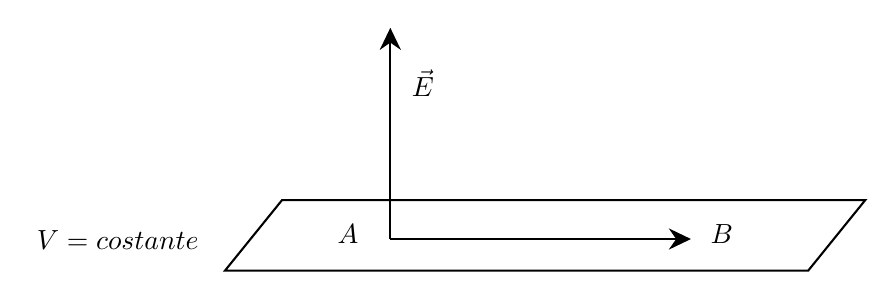
\begin{tikzpicture}[x=0.75pt,y=0.75pt,yscale=-1,xscale=1]
	%uncomment if require: \path (0,300); %set diagram left start at 0, and has height of 300

	%Shape: Parallelogram [id:dp65389199804943] 
	\draw   (203.5,153) -- (484.5,153) -- (457,187) -- (176,187) -- cycle ;
	%Straight Lines [id:da3668762040266511] 
	\draw    (397.5,171.77) -- (255.66,171.77) ;
	\draw [shift={(400.5,171.77)}, rotate = 180] [fill={rgb, 255:red, 0; green, 0; blue, 0 }  ][line width=0.08]  [draw opacity=0] (10.72,-5.15) -- (0,0) -- (10.72,5.15) -- (7.12,0) -- cycle    ;
	%Straight Lines [id:da939309199569287] 
	\draw    (255.66,73) -- (255.66,171.77) ;
	\draw [shift={(255.66,70)}, rotate = 90] [fill={rgb, 255:red, 0; green, 0; blue, 0 }  ][line width=0.08]  [draw opacity=0] (10.72,-5.15) -- (0,0) -- (10.72,5.15) -- (7.12,0) -- cycle    ;

	% Text Node
	\draw (235.33,169.42) node    {$A$};
	% Text Node
	\draw (415.33,169.42) node    {$B$};
	% Text Node
	\draw (271.33,96.42) node    {$\vec{E}$};
	% Text Node
	\draw (124.33,172.42) node    {$V=\text{costante}$};

	\end{tikzpicture}
\end{figure}
\FloatBarrier

\begin{align*}
	dV = \underbrace{V(B)-V(A)}_{=0} = \vec{\nabla} V\,d\vec{l} = -\vec{E} \cdot d\vec{l}
\end{align*}

Se ci spostiamo lungo la superficie equipotenziale, il potenziale non cambia e quindi il gradiente è ortogonale in ogni punto ad essa. Questa caratteristica si può generalizzare nel caso di una qualsiasi funzione. Il vettore gradiente di $f$ è sempre perpendicolare alle superfici $f_0$ di $f$ costante.
Nel caso di un campo elettrico generato da una carica, le superficie equipotenziali sono delle sfere centrate sulla carica stessa.
Se invece considero uno spostamento nella direzione del gradiente $d\vec{l}$ si ha:

\[
	dV = -\vec{E} \cdot d\vec{l} = |\vec{E}|\,|d\vec{l}|\cos \alpha
\]

Il caso di $ \alpha =0 $ è quello in cui otteniamo il massimo prodotto scalare. Ciò significa che se ci muoviamo nella direzione del gradiente di $f$, troviamo il massimo aumento di funzione $f$. Detto in altri termini, il vettore $ \vec{\nabla} f $ \emph{punta nella direzione di massima crescita della funzione}.

Concludiamo che il campo elettrostatico in ogni punto è perpendicolare alla superficie equipotenziale che passa per quel punto e il suo verso indica il verso di diminuzione del potenziale, visto il segno negativo. Dunque il campo elettrico è sempre diretto dal potenziale più alto a quello più basso. Tali superficie sono dunque ortogonali alle linee di forza.

Notiamo che se rappresentiamo le superfici equipotenziali con un certo passo fisso $ \Delta V $, le superficie equipotenziali si infittiscono nelle zone in cui il campo è maggiore; in un campo uniforme esse sono equispaziate.

\section{II Equazione di Maxwell (solo in regime stazionario)}

Il concetto di conservatività introdotto per i campi di forza si può estendere a un qualunque campo vettoriale. Abbiamo tuttavia studiato che se un campo elettrico è conservativo la sua circuitazione lungo un qualsiasi percorso chiuso è sempre zero.

\[
	\oint_{\gamma} \vec{E} \cdot d\vec{l} = 0 \qquad \forall \gamma \quad \text{chiusa}
\]

Per il teorema di Stokes:

\[
	0 = \oint_{\gamma} \vec{E} \cdot d\vec{l} =\int_{\Sigma}(\text{rot}\vec{E} )\cdot \vec{n} dS \implies \boxed{\text{rot}\vec{E} = 0}
\]

L'equazione ottenuta è la \textbf{II Equazione di Maxwell}. Mentre la prima vale in qualsiasi regime, \emph{la seconda vale solo in campi elettrostatici}. È possibile estenderla per i campi variabili nel tempo, non avremo più $0$ ma un altro termine. L'annullamento del rotore di un campo vettoriale in un qualunque punto dello spazio è una proprietà molto particolare. Se ciò accade diciamo che è un \textbf{campo vettoriale irrotazionale}.
$ \text{rot}\vec{v} =0 $ ovunque equivale a dire che il campo vettoriale è conservativo. Questo perché se il rotore è zero per il teorema di Stokes anche la circuitazione lo sarà.

Abbiamo visto che il legame fra $\vec{E}$ e il potenziale $V$ è pari a $ \vec{E} = - \text{grad}V $.
Anche questo è un modo per esprimere la conservatività di un campo. Quando si può scrivere un'espressione di questo tipo, il campo è automaticamente conservativo.
Abbiamo visto che:

\begin{gather*}
	\text{rot}\vec{v} = \vec{u}_x\left( \frac{\partial v_z}{\partial y} -\frac{\partial v_y}{\partial z}  \right)  +
	\vec{u}_y\left( \frac{\partial v_x}{\partial z} -\frac{\partial v_z}{\partial x}  \right)  +
	\vec{u}_z\left( \frac{\partial v_y}{\partial x} -\frac{\partial v_x}{\partial y}  \right) \\
	\text{rot}\vec{E} = \text{rot}(-\text{grad}V) = - \text{rot}(\text{grad}V) \\
	\text{grad}V = \frac{\partial V}{\partial x} \vec{u}_x + \frac{\partial V}{\partial y} \vec{u}_y + \frac{\partial V}{\partial z} \vec{u}_z \\
	\Downarrow \\
	\text{rot}\vec{E} = \vec{u}_x \left( \frac{\partial^2 V}{\partial z \partial y} - \frac{\partial^2 V}{\partial y \partial z}\right) + \vec{u}_y \left( \frac{\partial^2 V}{\partial z \partial x} - \frac{\partial^2 V}{\partial x \partial z}\right) + \vec{u}_z \left( \frac{\partial^2 V}{\partial y \partial x} - \frac{\partial^2 V}{\partial x \partial y}\right)
\end{gather*}

I termini tra parentesi sono tutti nulli per la proprietà delle derivate seconde miste di essere indipendenti dall'ordine di derivazione (\textbf{teorema di Schwarz}).
Quindi anche così si trova che il rotore è nullo e che \emph{un campo conservativo è irrotazionale}.

\[
	\vec{\nabla} \times (\vec{\nabla} f)=(\vec{\nabla} \times \vec{\nabla} ) f = 0
\]

Se moltiplico un vettore per se stesso il risultato è $0$, perché il prodotto vettoriale fra i vettori contiene il seno di $0$. In altre parole, l'applicazione successiva delle due operazioni di gradiente e di rotore dà risultato nullo.

Il fatto che $ \text{rot}\vec{E} =0 $ implica che abbia una struttura particolare, ossia, imponendo le componenti del rotore uguali a zero:

\begin{gather*}
	\frac{\partial E_z}{\partial y} = \frac{\partial E_y}{\partial z} \;\;\;\;\;\;\;
	\frac{\partial E_x}{\partial z} = \frac{\partial E_z}{\partial x} \;\;\;\;\;\;\;
	\frac{\partial E_y}{\partial x} = \frac{\partial E_x}{\partial y}
\end{gather*}

Un'altra considerazione importante è la seguente: se un campo $\vec{v}$ ha delle linee chiuse, allora non può essere conservativo, perché la circuitazione lungo quelle linee chiuse non sarebbe nullo.

\begin{figure}[htpb]
	\centering

	\tikzset{every picture/.style={line width=0.75pt}} %set default line width to 0.75pt        

	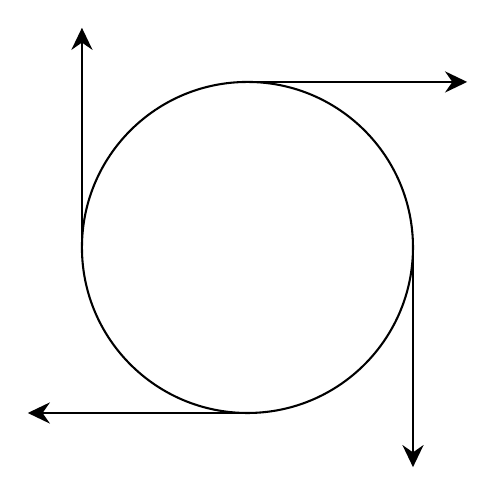
\begin{tikzpicture}[x=0.75pt,y=0.75pt,yscale=-1,xscale=1]
	%uncomment if require: \path (0,300); %set diagram left start at 0, and has height of 300

	%Shape: Circle [id:dp19640274429346416] 
	\draw   (184,145.75) .. controls (184,101.71) and (219.71,66) .. (263.75,66) .. controls (307.79,66) and (343.5,101.71) .. (343.5,145.75) .. controls (343.5,189.79) and (307.79,225.5) .. (263.75,225.5) .. controls (219.71,225.5) and (184,189.79) .. (184,145.75) -- cycle ;
	%Straight Lines [id:da389688705422198] 
	\draw    (366.59,66) -- (263.75,66) ;
	\draw [shift={(369.59,66)}, rotate = 180] [fill={rgb, 255:red, 0; green, 0; blue, 0 }  ][line width=0.08]  [draw opacity=0] (10.72,-5.15) -- (0,0) -- (10.72,5.15) -- (7.12,0) -- cycle    ;
	%Straight Lines [id:da45319967518017834] 
	\draw    (263.75,225.5) -- (160.91,225.5) ;
	\draw [shift={(157.91,225.5)}, rotate = 360] [fill={rgb, 255:red, 0; green, 0; blue, 0 }  ][line width=0.08]  [draw opacity=0] (10.72,-5.15) -- (0,0) -- (10.72,5.15) -- (7.12,0) -- cycle    ;
	%Straight Lines [id:da4667229649898803] 
	\draw    (343.5,248.59) -- (343.5,145.75) ;
	\draw [shift={(343.5,251.59)}, rotate = 270] [fill={rgb, 255:red, 0; green, 0; blue, 0 }  ][line width=0.08]  [draw opacity=0] (10.72,-5.15) -- (0,0) -- (10.72,5.15) -- (7.12,0) -- cycle    ;
	%Straight Lines [id:da9470975002641668] 
	\draw    (184,145.75) -- (184,42.91) ;
	\draw [shift={(184,39.91)}, rotate = 450] [fill={rgb, 255:red, 0; green, 0; blue, 0 }  ][line width=0.08]  [draw opacity=0] (10.72,-5.15) -- (0,0) -- (10.72,5.15) -- (7.12,0) -- cycle    ;

	\end{tikzpicture}
\end{figure}
\FloatBarrier

Il significato dell'operatore rotore è il seguente: esso ci dice sono i vortici, ci indica il piano in cui si svolgono e, in base al segno, ci dice il verso in cui ruotano.

\section{Equazioni di Poisson e di Laplace}

Essendo $\vec{E}$ conservativo possiamo esprimere il suo potenziale come $\vec{E} = -\vec{\nabla} V$. Inoltre, usando la I Equazione di Maxwell

\[
	\text{div}\vec{E} = \frac{\rho}{\varepsilon_0}\implies \vec{\nabla} \cdot (-\vec{\nabla} V)=\frac{\rho}{\varepsilon_0} \implies \nabla^2 V=-\frac{\rho}{\varepsilon_0}
\]

L'operatore $ \nabla^2 $ è noto come \textbf{operatore Laplaciano} o \textbf{operatore di Laplace}

\[
	\nabla^2 = \frac{\partial^2}{\partial x^2} + \frac{\partial^2}{\partial y^2} + \frac{\partial^2}{\partial z^2}
\]

Mentre l'ultima relazione è nota come \textbf{Equazione di Poisson}

\[
	\boxed{\nabla^2V = \frac{\partial^2 V}{\partial x^2} + \frac{\partial^2 V}{\partial y^2} + \frac{\partial^2 V}{\partial z^2} = - \frac{\rho(x,y,z)}{\varepsilon_0}}
\]

Se la densità di carica è nulla, ad esempio dentro un conduttore, l'equazione diventa nota come \textbf{Equazione di Laplace}:

\[
	\nabla^2 V=0
\]

L'integrazione di tale equazione con determinate condizioni al
contorno permette di determinare univocamente il potenziale $ V(x,y,z) $ e da questo il campo elettrico attraverso l'operazione di gradiente. In effetti in Analisi II si dimostra il cosiddetto \emph{teorema di unicità della soluzione dell'equazione di Poisson}, secondo il quale, se si impone al potenziale di annullarsi all'infinito insieme a tutte le sue derivate (e quindi è nullo all'infinito anche il campo) e si fissa una certa distribuzione di carica $ \rho (x,y,z)$ contenuta in una regione finita di spazio, la soluzione dell'equazione di Poisson è data da:

\[
	V(P)= \int_{\tau}\frac{\rho (x,y,z) d\tau}{4\pi \varepsilon_0 |\vec{r} -\vec{r'}|} = \int_{\tau} \frac{\rho (x,y,z) dx'dy'dz'}{4\pi \varepsilon_0 \sqrt{(x-x')^2 + (y-y')^2} +(z-z')^2}
\]

Se poniamo che il potenziale $V$ abbia un certo valore assegnato $V_s $ su $\Sigma$, condizione al contorno, allora si dimostra che la soluzione all'equazione di Poisson esiste ed è unica. Una volta che assegnamo le cariche dentro una certa superficie sigma, si dimostra che l'equazione ha soluzione unica.

Se facciamo tendere $\Sigma$ ad infinito, se fissiamo il valore del potenziale all'infinito ad un certo valore che scegliamo noi, se è diversa da zero in una regione limitata dello spazio e se imponiamo che il potenziale $V$ vada come $1/r$ quando ci allontaniamo verso l'infinito e che il modulo del campo elettrico decresce come $1/r^2$, allora anche in questo caso la soluzione dell'equazione esiste ed è unica.

In analisi matematica, quando un equazione soddisfa l'equazione di Laplace si dice \textbf{armonica}. Per le funzioni armoniche vale il teorema della media. Tale teorema dice che se prendiamo un punto $P$ e immaginiamo una sfera $ \Sigma  $ che lo circonda e la funzione è armonica, allora il valore che la funzione assume nel punto $O$ nel centro è uguale al valore medio di $V$ sulla sfera.
Se vale il teorema della media allora vuol dire che questa funzione non può assumere né minimi né massimi. In generale per le funzioni armoniche si può affermare che non hanno punti di minimo o massimo. Una volta stabilito che in una regione dello spazio il potenziale non ha minimi o massimi, nemmeno l'energia potenziale della carica ne ha. I punti di minimo di energia potenziale sono punti di equilibrio stabile. Ciò significa che in tale regione non ci sono punti di equilibrio né stabili né instabili. Se mettiamo la carica in un punto rimane ferma. Nella fisica delle particelle non è possibile usare solo campi elettrici per tenere ferme le cariche perché non si riesce mai a ottenere una zona di equilibrio. Per queste applicazioni si usano i campi magnetici. Per far sì che la materia rimanga stabile gli elettroni orbitano, questo perché le forze elettrostatiche non danno punti di equilibrio. La struttura della materia è stabile perché è una struttura dinamica.

\section{Condizioni al contorno per il campo elettrostatico}

Consideriamo il caso generale di una superficie $\Sigma$ di separazione fra due regioni dello spazio che chiameremo $1$ e $2$. Si tratta di mezzi differenti, ad esempio la regione $2$ potrebbe essere occupata da un conduttore mentre la $1$ essere vuota. Assumiamo che sulla superficie sia presente anche della carica elettrica positiva. Poniamo di conoscere la densità di carica superficiale in ogni punto della essa. Consideriamo in particolare un punto $P$ e i campi elettrici presenti \emph{in prossimità} del punto $P$ dal lato $1$ e dal lato $2$.

\begin{figure}[htpb]
	\centering

	\tikzset{every picture/.style={line width=0.75pt}} %set default line width to 0.75pt        

	\begin{tikzpicture}[x=0.75pt,y=0.75pt,yscale=-1,xscale=1]
	%uncomment if require: \path (0,300); %set diagram left start at 0, and has height of 300

	%Straight Lines [id:da9167485757937464] 
	\draw    (154,165) -- (483.5,165) ;
	%Shape: Circle [id:dp7785704410574901] 
	\draw  [fill={rgb, 255:red, 0; green, 0; blue, 0 }  ,fill opacity=1 ] (296.99,165.11) .. controls (296.99,163.45) and (298.34,162.11) .. (299.99,162.11) .. controls (301.65,162.11) and (302.99,163.45) .. (302.99,165.11) .. controls (302.99,166.77) and (301.65,168.11) .. (299.99,168.11) .. controls (298.34,168.11) and (296.99,166.77) .. (296.99,165.11) -- cycle ;
	%Straight Lines [id:da49790538469185663] 
	\draw    (299.99,165.11) -- (340.44,74.74) ;
	\draw [shift={(341.67,72)}, rotate = 474.11] [fill={rgb, 255:red, 0; green, 0; blue, 0 }  ][line width=0.08]  [draw opacity=0] (10.72,-5.15) -- (0,0) -- (10.72,5.15) -- (7.12,0) -- cycle    ;
	%Straight Lines [id:da5337472774971028] 
	\draw    (234.5,230) -- (297.86,167.22) ;
	\draw [shift={(299.99,165.11)}, rotate = 495.26] [fill={rgb, 255:red, 0; green, 0; blue, 0 }  ][line width=0.08]  [draw opacity=0] (10.72,-5.15) -- (0,0) -- (10.72,5.15) -- (7.12,0) -- cycle    ;

	% Text Node
	\draw (170,156) node    {$+$};
	% Text Node
	\draw (134,135) node    {$1$};
	% Text Node
	\draw (134,196) node    {$2$};
	% Text Node
	\draw (190,156) node    {$+$};
	% Text Node
	\draw (210,156) node    {$+$};
	% Text Node
	\draw (230,156) node    {$+$};
	% Text Node
	\draw (250,156) node    {$+$};
	% Text Node
	\draw (270,156) node    {$+$};
	% Text Node
	\draw (290,156) node    {$+$};
	% Text Node
	\draw (310,156) node    {$+$};
	% Text Node
	\draw (330,156) node    {$+$};
	% Text Node
	\draw (350,156) node    {$+$};
	% Text Node
	\draw (370,156) node    {$+$};
	% Text Node
	\draw (390,156) node    {$+$};
	% Text Node
	\draw (410,156) node    {$+$};
	% Text Node
	\draw (430,156) node    {$+$};
	% Text Node
	\draw (450,156) node    {$+$};
	% Text Node
	\draw (470,156) node    {$+$};
	% Text Node
	\draw (312.33,181) node    {$P$};
	% Text Node
	\draw (354.67,78.33) node    {$\vec{E}_{1}$};
	% Text Node
	\draw (269,223) node    {$\vec{E}_{2}$};
	% Text Node
	\draw (498.67,165) node    {$\Sigma $};

	\end{tikzpicture}
\end{figure}
\FloatBarrier

Vorremmo trovare un legame fra questi due campi elettrici in funzione della densità di carica superficiale $\sigma$. Tali legami sono detti \textbf{condizioni al contorno del campo elettrostatico}. A questo fine, sfruttiamo il fatto Che il campo elettrostatico è conservativo e che gode del teorema di Gauss.

Sia $\Sigma$ la superficie di separazione tra le regioni $1$ e $2$. Siano $E_1$ e $E_2$ i campi valutati in prossimità della superficie.

In prossimità della superficie possiamo assumerla piatta anziché curva. Consideriamo un percorso $\gamma$ chiuso come in figura, supponiamo inoltre $dl\gg dh $, ossia $dl$ è un infinitesimo di ordine superiore rispetto a $dh$.

\begin{figure}[htpb]
	\centering

	\tikzset{every picture/.style={line width=0.75pt}} %set default line width to 0.75pt        

	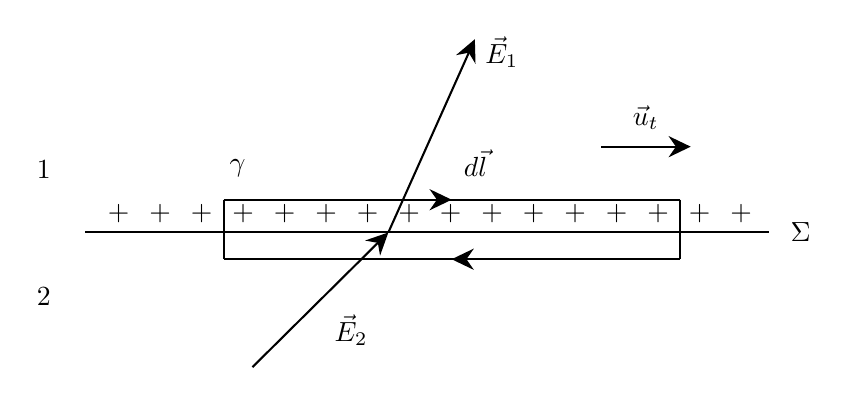
\begin{tikzpicture}[x=0.75pt,y=0.75pt,yscale=-1,xscale=1]
	%uncomment if require: \path (0,300); %set diagram left start at 0, and has height of 300

	%Straight Lines [id:da07387856013103389] 
	\draw    (174,185) -- (503.5,185) ;
	%Straight Lines [id:da261458001336919] 
	\draw    (319.99,185.11) -- (360.44,94.74) ;
	\draw [shift={(361.67,92)}, rotate = 474.11] [fill={rgb, 255:red, 0; green, 0; blue, 0 }  ][line width=0.08]  [draw opacity=0] (10.72,-5.15) -- (0,0) -- (10.72,5.15) -- (7.12,0) -- cycle    ;
	%Straight Lines [id:da3092345576534641] 
	\draw    (240.67,169.33) -- (460.33,169.33) ;
	\draw [shift={(350.5,169.33)}, rotate = 180] [fill={rgb, 255:red, 0; green, 0; blue, 0 }  ][line width=0.08]  [draw opacity=0] (10.72,-5.15) -- (0,0) -- (10.72,5.15) -- (7.12,0) -- cycle    ;
	%Straight Lines [id:da2617769489963089] 
	\draw    (240.67,198) -- (460.33,198) ;
	\draw [shift={(350.5,198)}, rotate = 0] [fill={rgb, 255:red, 0; green, 0; blue, 0 }  ][line width=0.08]  [draw opacity=0] (10.72,-5.15) -- (0,0) -- (10.72,5.15) -- (7.12,0) -- cycle    ;
	%Straight Lines [id:da294234843216612] 
	\draw    (460.33,169.33) -- (460.33,198) ;
	%Straight Lines [id:da09868490023182708] 
	\draw    (240.67,169.33) -- (240.67,198) ;
	%Straight Lines [id:da6190495865255945] 
	\draw    (422.66,143.77) -- (462.67,143.77) ;
	\draw [shift={(465.67,143.77)}, rotate = 180] [fill={rgb, 255:red, 0; green, 0; blue, 0 }  ][line width=0.08]  [draw opacity=0] (10.72,-5.15) -- (0,0) -- (10.72,5.15) -- (7.12,0) -- cycle    ;
	%Straight Lines [id:da15065625656460369] 
	\draw    (254.5,250) -- (317.86,187.22) ;
	\draw [shift={(319.99,185.11)}, rotate = 495.26] [fill={rgb, 255:red, 0; green, 0; blue, 0 }  ][line width=0.08]  [draw opacity=0] (10.72,-5.15) -- (0,0) -- (10.72,5.15) -- (7.12,0) -- cycle    ;

	% Text Node
	\draw (190,176) node    {$+$};
	% Text Node
	\draw (154,155) node    {$1$};
	% Text Node
	\draw (154,216) node    {$2$};
	% Text Node
	\draw (210,176) node    {$+$};
	% Text Node
	\draw (230,176) node    {$+$};
	% Text Node
	\draw (250,176) node    {$+$};
	% Text Node
	\draw (270,176) node    {$+$};
	% Text Node
	\draw (290,176) node    {$+$};
	% Text Node
	\draw (310,176) node    {$+$};
	% Text Node
	\draw (330,176) node    {$+$};
	% Text Node
	\draw (350,176) node    {$+$};
	% Text Node
	\draw (370,176) node    {$+$};
	% Text Node
	\draw (390,176) node    {$+$};
	% Text Node
	\draw (410,176) node    {$+$};
	% Text Node
	\draw (430,176) node    {$+$};
	% Text Node
	\draw (450,176) node    {$+$};
	% Text Node
	\draw (470,176) node    {$+$};
	% Text Node
	\draw (490,176) node    {$+$};
	% Text Node
	\draw (374.67,98.33) node    {$\vec{E}_{1}$};
	% Text Node
	\draw (302,232) node    {$\vec{E}_{2}$};
	% Text Node
	\draw (518.67,185) node    {$\Sigma $};
	% Text Node
	\draw (362,151.67) node    {$d\vec{l}$};
	% Text Node
	\draw (444,129.67) node    {$\vec{u}_{t}$};
	% Text Node
	\draw (247.33,154.33) node    {$\gamma $};

	\end{tikzpicture}
\end{figure}
\FloatBarrier

Ricordiamo inoltre la conservatività del campo $\vec{E}$:

\[
	\oint_{\gamma} \vec{E} \cdot d\vec{l} = 0
\]

Allora,

\begin{gather*}
	\oint_{\gamma} \vec{E} \cdot d\vec{l} \sim \vec{E}_1 \cdot (dl\vec{u}_t)+\vec{E}_2\cdot (-dl\vec{u}_t)=0 \implies \\
	(\vec{E}_1\cdot \vec{u}_t-\vec{E}_2\cdot \vec{u}_t)dl=0
\end{gather*}

Ma chiamando

\begin{gather*}
	E_{t1}= \vec{E}_1\cdot \vec{u}_t \\
	E_{t2}= \vec{E}_2\cdot \vec{u}_t
\end{gather*}

Si ottiene la seguente \textbf{condizione al contorno di tangenza}:

\[
	\boxed{E_{t1}=E_{t2}}
\]

Per ricavare informazioni sulle altre componenti del campo elettrico utilizziamo il teorema di Gauss. Useremo una superficie chiusa gaussiana $\Sigma_g$ di forma cilindrica a cavallo della superficie di separazione $\Sigma$ fra i due mezzi $1$ e $2$. Le basi sono parallele alla superficie sigma. Assumeremo che l'altezza del cilindro sia molto più piccola rispetto al raggio delle basi in modo da poter trascurare il flusso sulla superficie laterale.

\begin{figure}[htpb]
	\centering

	\tikzset{every picture/.style={line width=0.75pt}} %set default line width to 0.75pt        

	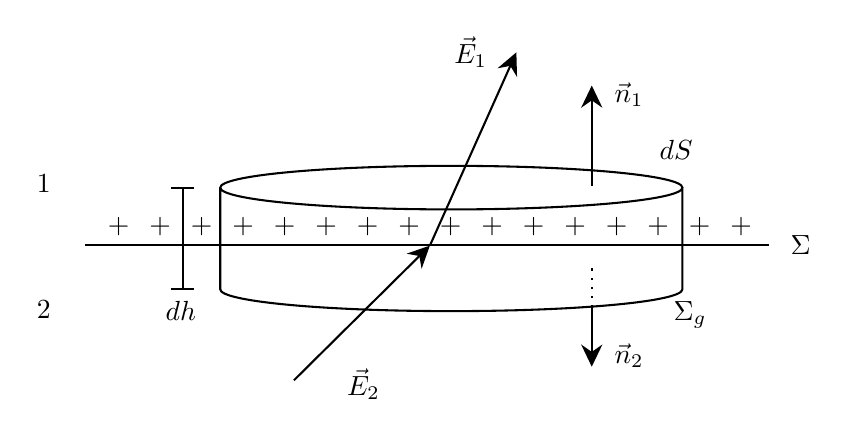
\begin{tikzpicture}[x=0.75pt,y=0.75pt,yscale=-1,xscale=1]
	%uncomment if require: \path (0,300); %set diagram left start at 0, and has height of 300

	%Straight Lines [id:da7426419768038623] 
	\draw    (159.33,194.33) -- (488.83,194.33) ;
	%Straight Lines [id:da13934423773510995] 
	\draw    (325.33,194.44) -- (365.77,104.07) ;
	\draw [shift={(367,101.33)}, rotate = 474.11] [fill={rgb, 255:red, 0; green, 0; blue, 0 }  ][line width=0.08]  [draw opacity=0] (10.72,-5.15) -- (0,0) -- (10.72,5.15) -- (7.12,0) -- cycle    ;
	%Shape: Can [id:dp7867133226586538] 
	\draw   (447,166.5) -- (447,215.5) .. controls (447,221.3) and (397.15,226) .. (335.67,226) .. controls (274.18,226) and (224.33,221.3) .. (224.33,215.5) -- (224.33,166.5) .. controls (224.33,160.7) and (274.18,156) .. (335.67,156) .. controls (397.15,156) and (447,160.7) .. (447,166.5) .. controls (447,172.3) and (397.15,177) .. (335.67,177) .. controls (274.18,177) and (224.33,172.3) .. (224.33,166.5) ;
	%Straight Lines [id:da48378000565482004] 
	\draw    (206.33,215.5) -- (206.33,166.5) ;
	\draw [shift={(206.33,166.5)}, rotate = 450] [color={rgb, 255:red, 0; green, 0; blue, 0 }  ][line width=0.75]    (0,5.59) -- (0,-5.59)   ;
	\draw [shift={(206.33,215.5)}, rotate = 450] [color={rgb, 255:red, 0; green, 0; blue, 0 }  ][line width=0.75]    (0,5.59) -- (0,-5.59)   ;
	%Straight Lines [id:da8031343165266469] 
	\draw    (403.33,165.77) -- (403.33,120.33) ;
	\draw [shift={(403.33,117.33)}, rotate = 450] [fill={rgb, 255:red, 0; green, 0; blue, 0 }  ][line width=0.08]  [draw opacity=0] (10.72,-5.15) -- (0,0) -- (10.72,5.15) -- (7.12,0) -- cycle    ;
	%Straight Lines [id:da922014640142611] 
	\draw    (403.33,249.77) -- (403.33,224.33) ;
	\draw [shift={(403.33,252.77)}, rotate = 270] [fill={rgb, 255:red, 0; green, 0; blue, 0 }  ][line width=0.08]  [draw opacity=0] (10.72,-5.15) -- (0,0) -- (10.72,5.15) -- (7.12,0) -- cycle    ;
	%Straight Lines [id:da24191265700742415] 
	\draw  [dash pattern={on 0.84pt off 2.51pt}]  (403.33,224.33) -- (403.33,204.33) ;
	%Straight Lines [id:da8876126540739697] 
	\draw    (259.83,259.33) -- (323.2,196.55) ;
	\draw [shift={(325.33,194.44)}, rotate = 495.26] [fill={rgb, 255:red, 0; green, 0; blue, 0 }  ][line width=0.08]  [draw opacity=0] (10.72,-5.15) -- (0,0) -- (10.72,5.15) -- (7.12,0) -- cycle    ;

	% Text Node
	\draw (175.33,185.33) node    {$+$};
	% Text Node
	\draw (139.33,164.33) node    {$1$};
	% Text Node
	\draw (139.33,225.33) node    {$2$};
	% Text Node
	\draw (195.33,185.33) node    {$+$};
	% Text Node
	\draw (215.33,185.33) node    {$+$};
	% Text Node
	\draw (235.33,185.33) node    {$+$};
	% Text Node
	\draw (255.33,185.33) node    {$+$};
	% Text Node
	\draw (275.33,185.33) node    {$+$};
	% Text Node
	\draw (295.33,185.33) node    {$+$};
	% Text Node
	\draw (315.33,185.33) node    {$+$};
	% Text Node
	\draw (335.33,185.33) node    {$+$};
	% Text Node
	\draw (355.33,185.33) node    {$+$};
	% Text Node
	\draw (375.33,185.33) node    {$+$};
	% Text Node
	\draw (395.33,185.33) node    {$+$};
	% Text Node
	\draw (415.33,185.33) node    {$+$};
	% Text Node
	\draw (435.33,185.33) node    {$+$};
	% Text Node
	\draw (455.33,185.33) node    {$+$};
	% Text Node
	\draw (475.33,185.33) node    {$+$};
	% Text Node
	\draw (345,101.33) node    {$\vec{E}_{1}$};
	% Text Node
	\draw (293.33,261) node    {$\vec{E}_{2}$};
	% Text Node
	\draw (504,194.33) node    {$\Sigma $};
	% Text Node
	\draw (444,148.33) node    {$dS$};
	% Text Node
	\draw (205.33,225.67) node    {$dh$};
	% Text Node
	\draw (421.33,121.67) node    {$\vec{n}_{1}$};
	% Text Node
	\draw (421.33,247.33) node    {$\vec{n}_{2}$};
	% Text Node
	\draw (450.67,227.67) node    {$\Sigma _{g}$};

	\end{tikzpicture}
\end{figure}
\FloatBarrier

La carica interna a $\Sigma_g$ è semplicemente pari a:

\[
	Q_{\text{tot}}^{\text{int a } \Sigma} = \sigma \,dS
\]

Applicando il teorema di Gauss quindi si ha:

\[
	\Phi_{\Sigma_g}(\vec{E}) = \int_{\Sigma_g} \vec{E} \cdot \vec{n} \, dS = \frac{Q_{\text{tot}}^{\text{int a } \Sigma}}{\varepsilon_0} = \frac{\sigma \,dS}{\varepsilon_0}
\]

Siccome le basi sono di area infinitesima possiamo eliminare l'integrale approssimando il flusso semplicemente come:

\begin{align*}
	\Phi_{\Sigma_g} (\vec{E}) &\simeq \vec{E}_1\vec{n}_1dS + \vec{E}_2\vec{n}_2dS \\
	\Phi_{\Sigma_g} &= (\vec{E}_1 \vec{n} - \vec{E}_2\vec{n} ) dS = \frac{\sigma \, dS}{\varepsilon_0} \tag*{$\vec{n} = \vec{n}_1\quad \vec{n} = - \vec{n}_2  $} \\
	& \qquad \underbrace{\vec{E}_1\vec{n}}_{E_{n1}} - \underbrace{\vec{E}_2\vec{n}}_{E_{n2}} = \frac{\sigma}{\varepsilon_0}
\end{align*}

La componente normale del campo elettrico presenta una discontinuità quando cambio mezzo legata alla densità di carica. Se non ci sono carice in mezzo ci aspettiamo che tutte le componenti del campo elettrico infatti siano continue.

\[
	\boxed{E_{n1} - E_{n2} = \frac{\sigma}{\varepsilon_0}}
\]

\section{Dipoli elettrici}

Chiamiamo \textbf{dipolo elettrico} una distribuzione di carica composta da una carica positiva e una carica negativa separate da una certa distanza rappresentata da un vettore d che punta sempre come in figura. 

\begin{figure}[htpb]
	\centering

	\tikzset{every picture/.style={line width=0.75pt}} %set default line width to 0.75pt        

	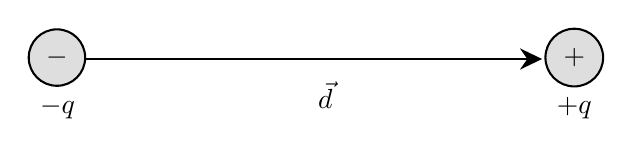
\begin{tikzpicture}[x=0.75pt,y=0.75pt,yscale=-1,xscale=1]
	%uncomment if require: \path (0,300); %set diagram left start at 0, and has height of 300

	%Straight Lines [id:da3549766989431007] 
	\draw    (208.33,171.44) -- (425.5,171.44) ;
	\draw [shift={(428.5,171.44)}, rotate = 180] [fill={rgb, 255:red, 0; green, 0; blue, 0 }  ][line width=0.08]  [draw opacity=0] (10.72,-5.15) -- (0,0) -- (10.72,5.15) -- (7.12,0) -- cycle    ;

	% Text Node
	\draw  [fill={rgb, 255:red, 222; green, 222; blue, 222 }  ,fill opacity=1 ]  (194.75, 170.75) circle [x radius= 13.6, y radius= 13.6]   ;
	\draw (194.75,170.75) node    {$-$};
	% Text Node
	\draw  [fill={rgb, 255:red, 222; green, 222; blue, 222 }  ,fill opacity=1 ]  (444, 170.75) circle [x radius= 13.9, y radius= 13.9]   ;
	\draw (444,170.75) node    {$+$};
	% Text Node
	\draw (195,195) node    {$-q$};
	% Text Node
	\draw (444,195) node    {$+q$};
	% Text Node
	\draw (324,189) node    {$\vec{d}$};

	\end{tikzpicture}
\end{figure}
\FloatBarrier

Le proprietà del dipolo possono essere riassunte da una quantità nota come \textbf{momento di dipolo}:

\[
	\vec{p} =q\,\vec{d}
\]

\paragraph{La materia e la polarizzazione.} Un atomo è costituito da un nucleo positivo attorno al quale orbita una nube di elettroni (carica negativa). Se applichiamo a un atomo un campo elettrico, il nucleo positivo vorrà andare nella sua stessa direzione, mentre l'intera nuvola negativa vorrà spostarsi verso sinistra. Il nucleo non sarà più corrispondente al baricentro nella nube negativa. Se immaginiamo di concentrare la nube nel baricentro, abbiamo due cariche separate da una certa distanza. Questo è un fenomeno che accade a tutti gli atomi, parziale separazione di carica. Tutta la materia reagisce ai campi elettrici in termine di polarizzazione.

\begin{figure}[htpb]
	\centering

	\tikzset{every picture/.style={line width=0.75pt}} %set default line width to 0.75pt        

	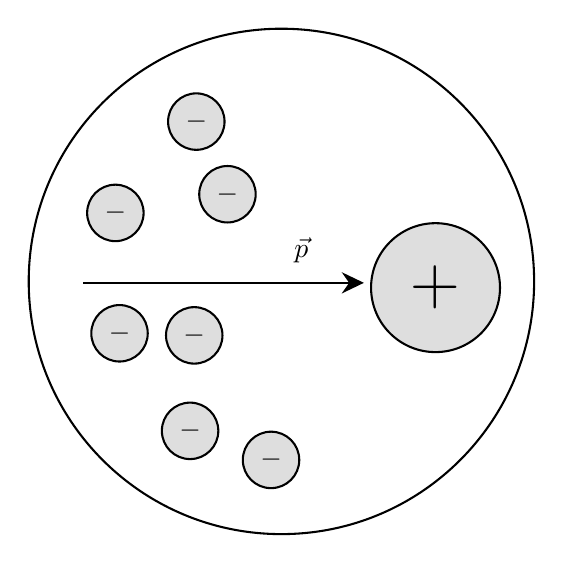
\begin{tikzpicture}[x=0.75pt,y=0.75pt,yscale=-1,xscale=1]
	%uncomment if require: \path (0,300); %set diagram left start at 0, and has height of 300

	%Shape: Circle [id:dp3548704480985345] 
	\draw   (172,160.75) .. controls (172,93.51) and (226.51,39) .. (293.75,39) .. controls (360.99,39) and (415.5,93.51) .. (415.5,160.75) .. controls (415.5,227.99) and (360.99,282.5) .. (293.75,282.5) .. controls (226.51,282.5) and (172,227.99) .. (172,160.75) -- cycle ;
	%Straight Lines [id:da6906697877581127] 
	\draw    (198.33,161.44) -- (330.5,161.44) ;
	\draw [shift={(333.5,161.44)}, rotate = 180] [fill={rgb, 255:red, 0; green, 0; blue, 0 }  ][line width=0.08]  [draw opacity=0] (10.72,-5.15) -- (0,0) -- (10.72,5.15) -- (7.12,0) -- cycle    ;

	% Text Node
	\draw  [fill={rgb, 255:red, 222; green, 222; blue, 222 }  ,fill opacity=1 ]  (368, 163.75) circle [x radius= 31.06, y radius= 31.06]   ;
	\draw (368,163.75) node  [font=\Huge]  {$+$};
	% Text Node
	\draw  [fill={rgb, 255:red, 222; green, 222; blue, 222 }  ,fill opacity=1 ]  (252.75, 83.75) circle [x radius= 13.6, y radius= 13.6]   ;
	\draw (252.75,83.75) node    {$-$};
	% Text Node
	\draw  [fill={rgb, 255:red, 222; green, 222; blue, 222 }  ,fill opacity=1 ]  (213.75, 127.75) circle [x radius= 13.6, y radius= 13.6]   ;
	\draw (213.75,127.75) node    {$-$};
	% Text Node
	\draw  [fill={rgb, 255:red, 222; green, 222; blue, 222 }  ,fill opacity=1 ]  (267.75, 118.75) circle [x radius= 13.6, y radius= 13.6]   ;
	\draw (267.75,118.75) node    {$-$};
	% Text Node
	\draw  [fill={rgb, 255:red, 222; green, 222; blue, 222 }  ,fill opacity=1 ]  (215.75, 185.75) circle [x radius= 13.6, y radius= 13.6]   ;
	\draw (215.75,185.75) node    {$-$};
	% Text Node
	\draw  [fill={rgb, 255:red, 222; green, 222; blue, 222 }  ,fill opacity=1 ]  (249.75, 232.75) circle [x radius= 13.6, y radius= 13.6]   ;
	\draw (249.75,232.75) node    {$-$};
	% Text Node
	\draw  [fill={rgb, 255:red, 222; green, 222; blue, 222 }  ,fill opacity=1 ]  (251.75, 186.75) circle [x radius= 13.6, y radius= 13.6]   ;
	\draw (251.75,186.75) node    {$-$};
	% Text Node
	\draw  [fill={rgb, 255:red, 222; green, 222; blue, 222 }  ,fill opacity=1 ]  (288.75, 246.75) circle [x radius= 13.6, y radius= 13.6]   ;
	\draw (288.75,246.75) node    {$-$};
	% Text Node
	\draw (303.34,146) node    {$\vec{p}$};

	\end{tikzpicture}
\end{figure}
\FloatBarrier

\paragraph{Potenziale elettrico generato da un bipolo.} Supponiamo di avere un bipolo fatto come in figura e di voler calcolare Il potenziale elettrostatico da esso generato in un punto $P$. Questo si può calcolare con il principio di sovrapposizione degli effetti, pur di conoscere la distanza del punto $P$ dalle cariche:

\[
	V(P)=\frac{q}{4\pi \varepsilon_0 r_1} - \frac{q}{4\pi \varepsilon_0 r_2} = \frac{q(r_2-r_1  )}{4\pi \varepsilon_0 r_1 r_2}
\]

Vogliamo tuttavia trovare un'approssimazione che ci dica come varia questo potenziale asintoticamente, allontanandoci molto.

\begin{figure}[htpb]
	\centering

	\tikzset{every picture/.style={line width=0.75pt}} %set default line width to 0.75pt        

	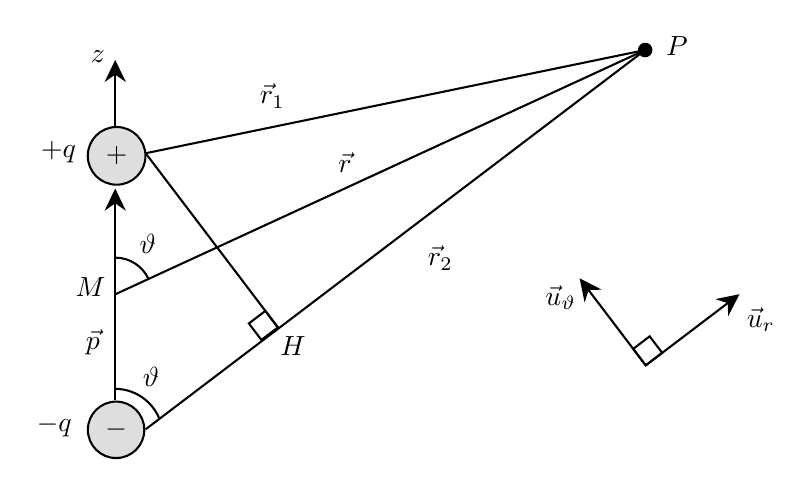
\begin{tikzpicture}[x=0.75pt,y=0.75pt,yscale=-1,xscale=1]
	%uncomment if require: \path (0,300); %set diagram left start at 0, and has height of 300

	%Straight Lines [id:da4699866327560356] 
	\draw    (232.33,235.44) -- (232.33,136.5) ;
	\draw [shift={(232.33,133.5)}, rotate = 450] [fill={rgb, 255:red, 0; green, 0; blue, 0 }  ][line width=0.08]  [draw opacity=0] (10.72,-5.15) -- (0,0) -- (10.72,5.15) -- (7.12,0) -- cycle    ;
	%Straight Lines [id:da36083572492704663] 
	\draw    (232.33,105.44) -- (232.33,74.5) ;
	\draw [shift={(232.33,71.5)}, rotate = 450] [fill={rgb, 255:red, 0; green, 0; blue, 0 }  ][line width=0.08]  [draw opacity=0] (10.72,-5.15) -- (0,0) -- (10.72,5.15) -- (7.12,0) -- cycle    ;
	%Shape: Circle [id:dp40738493154038635] 
	\draw  [fill={rgb, 255:red, 0; green, 0; blue, 0 }  ,fill opacity=1 ] (484.66,66.77) .. controls (484.66,65.12) and (486,63.77) .. (487.66,63.77) .. controls (489.32,63.77) and (490.66,65.12) .. (490.66,66.77) .. controls (490.66,68.43) and (489.32,69.77) .. (487.66,69.77) .. controls (486,69.77) and (484.66,68.43) .. (484.66,66.77) -- cycle ;
	%Straight Lines [id:da5192933348938815] 
	\draw    (247,116.5) -- (487.66,66.77) ;
	%Straight Lines [id:da6350346320756566] 
	\draw    (247,249.5) -- (487.66,66.77) ;
	%Straight Lines [id:da896914496459934] 
	\draw    (232.33,184.47) -- (487.66,66.77) ;
	%Straight Lines [id:da8701075468927895] 
	\draw    (247,116.5) -- (310.7,200.4) ;
	%Shape: Square [id:dp13013832557219307] 
	\draw   (296.72,198.51) -- (304.66,192.46) -- (310.7,200.4) -- (302.77,206.44) -- cycle ;
	%Shape: Arc [id:dp8640724180283808] 
	\draw  [draw opacity=0] (232.48,166.8) .. controls (239.49,166.86) and (245.53,171) .. (248.33,176.97) -- (232.33,184.47) -- cycle ; \draw   (232.48,166.8) .. controls (239.49,166.86) and (245.53,171) .. (248.33,176.97) ;
	%Shape: Arc [id:dp9712219715449886] 
	\draw  [draw opacity=0] (232.37,230) .. controls (242.02,230.08) and (250.26,236.07) .. (253.65,244.53) -- (232.18,253.11) -- cycle ; \draw   (232.37,230) .. controls (242.02,230.08) and (250.26,236.07) .. (253.65,244.53) ;
	%Straight Lines [id:da2281231996191373] 
	\draw    (487.93,218.7) -- (530.72,186.21) ;
	\draw [shift={(533.11,184.4)}, rotate = 502.79] [fill={rgb, 255:red, 0; green, 0; blue, 0 }  ][line width=0.08]  [draw opacity=0] (10.72,-5.15) -- (0,0) -- (10.72,5.15) -- (7.12,0) -- cycle    ;
	%Straight Lines [id:da5625694167837756] 
	\draw    (457.91,179.16) -- (487.93,218.7) ;
	\draw [shift={(456.1,176.77)}, rotate = 52.79] [fill={rgb, 255:red, 0; green, 0; blue, 0 }  ][line width=0.08]  [draw opacity=0] (10.72,-5.15) -- (0,0) -- (10.72,5.15) -- (7.12,0) -- cycle    ;
	%Shape: Square [id:dp9703624883708826] 
	\draw   (481.89,210.76) -- (489.83,204.72) -- (495.87,212.66) -- (487.93,218.7) -- cycle ;

	% Text Node
	\draw  [fill={rgb, 255:red, 222; green, 222; blue, 222 }  ,fill opacity=1 ]  (232.75, 249.75) circle [x radius= 13.6, y radius= 13.6]   ;
	\draw (232.75,249.75) node    {$-$};
	% Text Node
	\draw  [fill={rgb, 255:red, 222; green, 222; blue, 222 }  ,fill opacity=1 ]  (233, 117.75) circle [x radius= 13.9, y radius= 13.9]   ;
	\draw (233,117.75) node    {$+$};
	% Text Node
	\draw (203,248) node    {$-q$};
	% Text Node
	\draw (205,116) node    {$+q$};
	% Text Node
	\draw (221.6,207.6) node    {$\vec{p}$};
	% Text Node
	\draw (224,70) node    {$z$};
	% Text Node
	\draw (503,65) node    {$P$};
	% Text Node
	\draw (308,89) node    {$\vec{r}_{1}$};
	% Text Node
	\draw (389,167) node    {$\vec{r}_{2}$};
	% Text Node
	\draw (343,121) node    {$\vec{r}$};
	% Text Node
	\draw (248,160) node    {$\vartheta $};
	% Text Node
	\draw (249.6,224.4) node    {$\vartheta $};
	% Text Node
	\draw (220.4,181.2) node    {$M$};
	% Text Node
	\draw (318,209.2) node    {$H$};
	% Text Node
	\draw (543.4,196.6) node    {$\vec{u}_{r}$};
	% Text Node
	\draw (447,186.2) node    {$\vec{u}_{\vartheta }$};

	\end{tikzpicture}
\end{figure}
\FloatBarrier

Consideriamo il punto medio $M$ della distanza fra le cariche e supponiamo che $r = MP$ (rappresentato in figura) sia molto maggiore della separazione $d$ fra le due cariche: $ r \gg d $.
Sia $ \vartheta  $ l'angolo formato da $r$ e $d$. Se immaginiamo che il punto $P$ si trovi a distanza infinita, $r$ ed $ r_2  $ finiscono per essere paralleli ed anche l'angolo formato da $d$ ed $ r_2  $ sarà pari a $ \vartheta  $.
All'infinito possiamo dire che:

\[
	\left. \begin{array}{r}
	 	PH \simeq r_1  \\
		r_2 -r_1  \simeq + d\,\cos \vartheta \\
		r_1 r_2 \simeq r^2
	\end{array} \right\} V(P) \simeq \frac{\overbrace{qd}^p\cos \vartheta}{4\pi \varepsilon_0 r^2} = \frac{\overbrace{p\cos \vartheta}^{\vec{p} \cdot \vec{u}_r}}{4\pi \varepsilon_0 r^2} = \frac{\vec{p} \cdot \vec{u}_r}{4\pi \varepsilon_0 r^2}
\]

A grandi distanze dal dipolo quindi il potenziale da esso generato sarà:

\[
	\boxed{V(P) = \frac{\vec{p} \cdot \vec{u}_r}{4\pi \varepsilon_0 r^2}} \qquad  \propto \frac{1}{r^2}
\]

Notiamo come l'unica grandezza caratteristica del dipolo è il momento $ \vec{p}  $ e non $q$ e $d$ separatamente: ciò indica che da misure di potenziale possiamo ricavare informazioni su $\vec{p}$, ma non sulla costituzione del sistema.
Poniamoci in un sistema di coordinate in cui chiamiamo $ \vec{u}_r $ il versore diretto come $ r $ e $ \vec{u}_{\vartheta} $ quello perpendicolare a $ \vec{u}_r $. Si avrà che il campo elettrico generato dal dipolo sarà:

\begin{align*}
	\vec{E} &= - \vec{\nabla} V = -\frac{\partial V}{\partial r} \vec{u}_r - \frac{1}{r} \frac{\partial V}{\partial \vartheta} \vec{u}_{\vartheta} \tag*{regola della catena}\\
	&= \frac{2p\cos \vartheta}{4\pi \varepsilon_0 r^3} \vec{u}_r + \frac{p\sin \vartheta}{4\pi \varepsilon_0 r^3} \vec{u}_{\vartheta} \tag*{derivando} \\
	&= \frac{3p\cos \vartheta}{4\pi \varepsilon_0 r^3}\vec{u}_r - \frac{\vec{p}}{4\pi \varepsilon_0 r^3} \tag*{$\vec{p} =p\cos \vartheta \vec{u}_r - p \sin \vartheta \vec{u}_{\vartheta}$} \\
	&= \frac{1}{4\pi \varepsilon_0 r^3}[3(\vec{p} \cdot \vec{u}_r)\vec{u}_r-\vec{p}] \qquad \propto \frac{1}{r^3}
\end{align*}

\paragraph{Andamento asintotico e sviluppo in serie di multipoli.}Riassumiamo nella seguente tabella gli andamenti asintotici del potenziale e del campo elettrico a distanza infinita per generati rispettivamente da una carica puntiforme e da un bipolo.

\begin{table}[htpb]
	\centering
	\begin{tabular}{r|c|c}
		& carica puntiforme & dipolo \\
		\hline
		$V(r)$ & $ \propto 1/r $ & $ \propto 1/r^2  $ \\
		\hline
		$ |\vec{E} (r)| $ & $ \propto 1/r^2 $ & $ \propto 1/r^3  $
	\end{tabular}
\end{table}

Potremmo anche considerare un quadripolo, e in quel caso si avrebbe:

\[
	|\vec{E} (r)| \propto 1/r^4 \qquad V(r) \propto 1/r^3
\]

Quando dobbiamo calcolare il potenziale prodotto da una certa distribuzione di carica $ \rho  $ abbiamo due approcci.

\begin{itemize}
	\item Uno si basa su una formula precisa calcolata in precedenza utilizzando il principio di sovrapposizione degli effetti:
	\[
		V(P) = \int_{\tau}\frac{\rho (x',y',z') d\tau}{4\pi \varepsilon_0 |\vec{r} - \vec{r'}|}
	\]
	\item Un altro approccio si basa su una approssimazione in serie del potenziale. Abbiamo visto che il potenziale può andare come $1/r$, $1/r^2$ e via dicendo. Allora poniamo che $V(P)$ si possa vedere come una sommatoria:
	\[
		V(P) = \sum_{i=1}^n \frac{k_i}{r^i}
	\]
\end{itemize}

Il terimine $i=1$ corrisponde al caso in cui abbiamo una carica puntiforme. Facendo uno sviluppo in serie del potenziale, lo vediamo come somma dei potenziali generati dalla carica puntiforme, multiforme, quadriforme ecc... Se la distribuzione di carica ha una carica totale diversa da zero, il termine preponderante a grande distanza è quello della carica puntiforme. La funzione $1/r$ decresce più lentamente inoltre rispetto agli altri termini, che diventano insignificanti. Se la distribuzione di carica ha una carica totale pari a $0$, il termine di carica puntiforme scompare, ma abbiamo un dipolo. A questo punto il termine che diventa preponderante è quello del dipolo, $1/r^2$. Nello sviluppo in serie \emph{ci si ferma al primo termine più importante degli altri}, che decresce più lentamente. Questo sviluppo in serie prende il nome di \textbf{sviluppo in serie di multipoli}. Quindi non sempre l'andamento del campo elettrico è quello di una carica puntiforme.

\section{Interazione fra un dipolo e un campo elettrico}

\subsection{Caso I: Campo elettrico uniforme}

I seguenti ragionamenti sono attuati basandosi sull'ipotesi che il bipolo di cui ci stiamo occupando sia \emph{rigido}, ossia che la distanza fra la carica positiva e quella negativa sia sempre costante. Consideriamo il caso di un dipolo immerso in un campo elettrico uniforme. Questo significa che il vettore $\vec{E}$ è costante in tutti i punti dello spazio.

\begin{figure}[htpb]
	\centering

	\tikzset{every picture/.style={line width=0.75pt}} %set default line width to 0.75pt        

	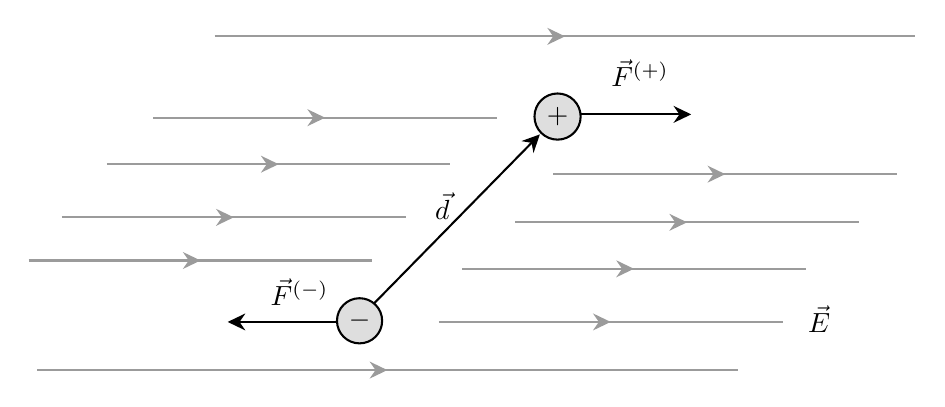
\begin{tikzpicture}[x=0.75pt,y=0.75pt,yscale=-0.8,xscale=0.8]
	%uncomment if require: \path (0,300); %set diagram left start at 0, and has height of 300

	%Straight Lines [id:da3173086254193631] 
	\draw    (245.33,223.44) -- (343.23,123.64) ;
	\draw [shift={(345.33,121.5)}, rotate = 494.45] [fill={rgb, 255:red, 0; green, 0; blue, 0 }  ][line width=0.08]  [draw opacity=0] (10.72,-5.15) -- (0,0) -- (10.72,5.15) -- (7.12,0) -- cycle    ;
	%Straight Lines [id:da3908064807839329] 
	\draw    (357.33,109.44) -- (433.5,109.44) ;
	\draw [shift={(436.5,109.44)}, rotate = 180] [fill={rgb, 255:red, 0; green, 0; blue, 0 }  ][line width=0.08]  [draw opacity=0] (10.72,-5.15) -- (0,0) -- (10.72,5.15) -- (7.12,0) -- cycle    ;
	%Straight Lines [id:da3972074201231366] 
	\draw    (160.33,234.44) -- (236.5,234.44) ;
	\draw [shift={(157.33,234.44)}, rotate = 0] [fill={rgb, 255:red, 0; green, 0; blue, 0 }  ][line width=0.08]  [draw opacity=0] (10.72,-5.15) -- (0,0) -- (10.72,5.15) -- (7.12,0) -- cycle    ;
	%Straight Lines [id:da19936120489500797] 
	\draw [color={rgb, 255:red, 155; green, 155; blue, 155 }  ,draw opacity=1 ]   (112.5,111.44) -- (319.5,111.44) ;
	\draw [shift={(216,111.44)}, rotate = 180] [fill={rgb, 255:red, 155; green, 155; blue, 155 }  ,fill opacity=1 ][line width=0.08]  [draw opacity=0] (10.72,-5.15) -- (0,0) -- (10.72,5.15) -- (7.12,0) -- cycle    ;
	%Straight Lines [id:da5411513941269097] 
	\draw [color={rgb, 255:red, 155; green, 155; blue, 155 }  ,draw opacity=1 ]   (84.5,139.44) -- (291.5,139.44) ;
	\draw [shift={(188,139.44)}, rotate = 180] [fill={rgb, 255:red, 155; green, 155; blue, 155 }  ,fill opacity=1 ][line width=0.08]  [draw opacity=0] (10.72,-5.15) -- (0,0) -- (10.72,5.15) -- (7.12,0) -- cycle    ;
	%Straight Lines [id:da47310294529851005] 
	\draw [color={rgb, 255:red, 155; green, 155; blue, 155 }  ,draw opacity=1 ]   (57.5,171.44) -- (264.5,171.44) ;
	\draw [shift={(161,171.44)}, rotate = 180] [fill={rgb, 255:red, 155; green, 155; blue, 155 }  ,fill opacity=1 ][line width=0.08]  [draw opacity=0] (10.72,-5.15) -- (0,0) -- (10.72,5.15) -- (7.12,0) -- cycle    ;
	%Straight Lines [id:da33896527031281387] 
	\draw [color={rgb, 255:red, 155; green, 155; blue, 155 }  ,draw opacity=1 ]   (37.5,197.44) -- (244.5,197.44) ;
	\draw [shift={(141,197.44)}, rotate = 180] [fill={rgb, 255:red, 155; green, 155; blue, 155 }  ,fill opacity=1 ][line width=0.08]  [draw opacity=0] (10.72,-5.15) -- (0,0) -- (10.72,5.15) -- (7.12,0) -- cycle    ;
	%Straight Lines [id:da6784200085632801] 
	\draw [color={rgb, 255:red, 155; green, 155; blue, 155 }  ,draw opacity=1 ]   (42.5,263.44) -- (464.5,263.44) ;
	\draw [shift={(253.5,263.44)}, rotate = 180] [fill={rgb, 255:red, 155; green, 155; blue, 155 }  ,fill opacity=1 ][line width=0.08]  [draw opacity=0] (10.72,-5.15) -- (0,0) -- (10.72,5.15) -- (7.12,0) -- cycle    ;
	%Straight Lines [id:da7175663365447602] 
	\draw [color={rgb, 255:red, 155; green, 155; blue, 155 }  ,draw opacity=1 ]   (284.5,234.44) -- (491.5,234.44) ;
	\draw [shift={(388,234.44)}, rotate = 180] [fill={rgb, 255:red, 155; green, 155; blue, 155 }  ,fill opacity=1 ][line width=0.08]  [draw opacity=0] (10.72,-5.15) -- (0,0) -- (10.72,5.15) -- (7.12,0) -- cycle    ;
	%Straight Lines [id:da5808798540953077] 
	\draw [color={rgb, 255:red, 155; green, 155; blue, 155 }  ,draw opacity=1 ]   (298.5,202.44) -- (505.5,202.44) ;
	\draw [shift={(402,202.44)}, rotate = 180] [fill={rgb, 255:red, 155; green, 155; blue, 155 }  ,fill opacity=1 ][line width=0.08]  [draw opacity=0] (10.72,-5.15) -- (0,0) -- (10.72,5.15) -- (7.12,0) -- cycle    ;
	%Straight Lines [id:da03928239258857458] 
	\draw [color={rgb, 255:red, 155; green, 155; blue, 155 }  ,draw opacity=1 ]   (330.5,174.44) -- (537.5,174.44) ;
	\draw [shift={(434,174.44)}, rotate = 180] [fill={rgb, 255:red, 155; green, 155; blue, 155 }  ,fill opacity=1 ][line width=0.08]  [draw opacity=0] (10.72,-5.15) -- (0,0) -- (10.72,5.15) -- (7.12,0) -- cycle    ;
	%Straight Lines [id:da7787315920071702] 
	\draw [color={rgb, 255:red, 155; green, 155; blue, 155 }  ,draw opacity=1 ]   (353.5,145.44) -- (560.5,145.44) ;
	\draw [shift={(457,145.44)}, rotate = 180] [fill={rgb, 255:red, 155; green, 155; blue, 155 }  ,fill opacity=1 ][line width=0.08]  [draw opacity=0] (10.72,-5.15) -- (0,0) -- (10.72,5.15) -- (7.12,0) -- cycle    ;
	%Straight Lines [id:da9988803146962861] 
	\draw [color={rgb, 255:red, 155; green, 155; blue, 155 }  ,draw opacity=1 ]   (149.5,62.44) -- (571.5,62.44) ;
	\draw [shift={(360.5,62.44)}, rotate = 180] [fill={rgb, 255:red, 155; green, 155; blue, 155 }  ,fill opacity=1 ][line width=0.08]  [draw opacity=0] (10.72,-5.15) -- (0,0) -- (10.72,5.15) -- (7.12,0) -- cycle    ;

	% Text Node
	\draw  [fill={rgb, 255:red, 222; green, 222; blue, 222 }  ,fill opacity=1 ]  (236.75, 233.75) circle [x radius= 13.6, y radius= 13.6]   ;
	\draw (236.75,233.75) node    {$-$};
	% Text Node
	\draw  [fill={rgb, 255:red, 222; green, 222; blue, 222 }  ,fill opacity=1 ]  (356, 110.75) circle [x radius= 13.9, y radius= 13.9]   ;
	\draw (356,110.75) node    {$+$};
	% Text Node
	\draw (286.6,164.6) node    {$\vec{d}$};
	% Text Node
	\draw (405.6,84.6) node    {$\vec{F}^{( +)}$};
	% Text Node
	\draw (200.6,216.6) node    {$\vec{F}^{( -)}$};
	% Text Node
	\draw (513.6,232.6) node    {$\vec{E}$};

	\end{tikzpicture}
\end{figure}
\FloatBarrier

\[
	\vec{F}^{(+)} = q\vec{E}_0 \qquad \vec{F}^{(-)} = -q\vec{E}_0 \qquad \implies \qquad \boxed{\vec{R} = 0}
\]

Possiamo dire che se immergiamo un dipolo in un campo elettrico uniforme, la risultante delle forze è nulla e quindi anche l'accelerazione del centro di massa. Ricordando che il momento di una forza rispetto a un polo $ o $ vale:

\[
	\vec{M}^{(o)} = \vec{r} \times \vec{R}
\]

Si dimostra che nel caso in cui un sistema di forze è costituito da una coppia di forze $-\vec{F}$ e $\vec{F}$ disposte in direzione tale per cui la risultante $\vec{R}$ sia nulla, come in questo caso, $\vec{M}$ \emph{non dipende dalla scelta del polo}. Scegliamo quindi a nostra preferenza come polo il punto $O$, coincidente con la carica negativa. In questo caso il contributo del momento delle forze in $-q$ è nullo e si ha:

\[
	\vec{M} =\vec{d} \times \vec{F}^{(+)} = \vec{d} \times q\vec{E}_0 = q\vec{d} \times \vec{E}_0 = \boxed{\vec{M} = \vec{p} \times \vec{E}}
\]

Troviamo così il \textbf{momento di dipolo elettrico}. Il verso del momento dice anche il senso di rotazione (oraria in questo caso) che le forze impongono. L'effetto delle forze è quello di portare il dipolo allineato con il campo elettrico, poiché dato che il momento delle forze si annulla proprio in queste condizioni.

\subsection{Caso II: Campo elettrico non uniforme}

Consideriamo il caso in cui il campo elettrico non è uniforme.
In tali condizioni la risultante delle forze non è zero. Assumiamo che la distanza tra le due cariche sia piccola, sostanzialmente infinitesima.

\[
	\vec{d} =dx\vec{u}_x + dy\vec{u}_y+dz\vec{u}_z
\]

Il campo elettrico generato su $+q$ e $-q$ sarà rispettivamente:

\begin{align*}
	\vec{E}^{(-)} &= \vec{E} (x,y,z) \\
	\vec{E}^{(+)} &= \vec{E} (x+dx,y+dy,z+dz)
\end{align*}

\begin{figure}[htpb]
	\centering

	\tikzset{every picture/.style={line width=0.75pt}} %set default line width to 0.75pt        

	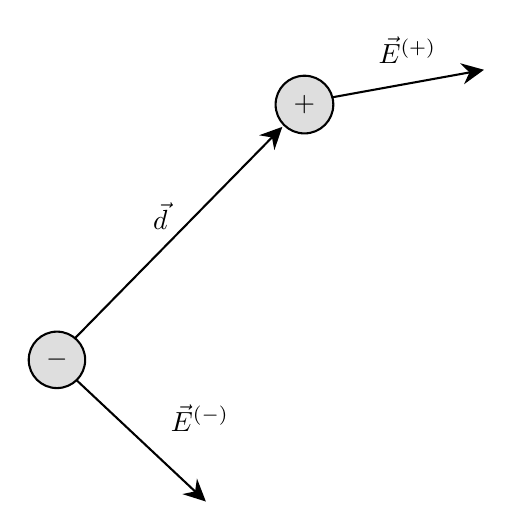
\begin{tikzpicture}[x=0.75pt,y=0.75pt,yscale=-1,xscale=1]
	%uncomment if require: \path (0,300); %set diagram left start at 0, and has height of 300

	%Straight Lines [id:da6757843094824549] 
	\draw    (261.33,198.44) -- (359.23,98.64) ;
	\draw [shift={(361.33,96.5)}, rotate = 494.45] [fill={rgb, 255:red, 0; green, 0; blue, 0 }  ][line width=0.08]  [draw opacity=0] (10.72,-5.15) -- (0,0) -- (10.72,5.15) -- (7.12,0) -- cycle    ;
	%Straight Lines [id:da6715254387985528] 
	\draw    (373.33,84.44) -- (455.55,69.54) ;
	\draw [shift={(458.5,69)}, rotate = 529.72] [fill={rgb, 255:red, 0; green, 0; blue, 0 }  ][line width=0.08]  [draw opacity=0] (10.72,-5.15) -- (0,0) -- (10.72,5.15) -- (7.12,0) -- cycle    ;
	%Straight Lines [id:da506216469916128] 
	\draw    (322.31,274.95) -- (252.5,209.44) ;
	\draw [shift={(324.5,277)}, rotate = 223.18] [fill={rgb, 255:red, 0; green, 0; blue, 0 }  ][line width=0.08]  [draw opacity=0] (10.72,-5.15) -- (0,0) -- (10.72,5.15) -- (7.12,0) -- cycle    ;

	% Text Node
	\draw  [fill={rgb, 255:red, 222; green, 222; blue, 222 }  ,fill opacity=1 ]  (252.75, 208.75) circle [x radius= 13.6, y radius= 13.6]   ;
	\draw (252.75,208.75) node    {$-$};
	% Text Node
	\draw  [fill={rgb, 255:red, 222; green, 222; blue, 222 }  ,fill opacity=1 ]  (372, 85.75) circle [x radius= 13.9, y radius= 13.9]   ;
	\draw (372,85.75) node    {$+$};
	% Text Node
	\draw (302.6,139.6) node    {$\vec{d}$};
	% Text Node
	\draw (421.6,59.6) node    {$\vec{E}^{( +)}$};
	% Text Node
	\draw (321.6,236.6) node    {$\vec{E}^{( -)}$};

	\end{tikzpicture}
\end{figure}
\FloatBarrier

Otteniamo allora che la risultante delle forze è pari a:

\[
	\vec{R} = q\left( \vec{E}^{(+)} - \vec{E}^{(-)}\right) = q\left[ \vec{E} (x+dx,y+dy,z+dz) - \vec{E} (x,y,z) \right]
\]

Procediamo con il ragionamento concentrandoci sulla componente $R_x$ della risultante, con la consapevolezza che esso è analogo per le altri componenti e che le conclusioni a cui arriveremo potranno essere estese a $R_y$ e $R_z$.

\begin{align*}
	R_x &=  q [ \underbrace{E_x  (x+dx,y+dy,z+dz)}_{E_x(x,y,z) +dE_x} - E_x  (x,y,z) ]  \tag*{teo. differenziale totale} \\
	&= q [E_x  (x,y,z) + dE_x - E_x  (x,y,z)] = q[dE_x ] \\
	&= q\left[ \frac{\partial E_x}{\partial x} dx + \frac{\partial E_x}{\partial y} dy + \frac{\partial E_x}{\partial z} dz \right] \\
	&= q \left[ \vec{\nabla} E_x \cdot \vec{d} \right] = \vec{p} \cdot \vec{\nabla} E_x
\end{align*}

Possiamo vedere $\vec{p} \cdot \vec{\nabla}$ come un unico operatore e scrivere:

\begin{gather*}
	R_x  = \left( \vec{p} \cdot \vec{\nabla}  \right)  E_x \qquad R_y  = \left( \vec{p} \cdot \vec{\nabla}  \right)  E_y \qquad R_z  = \left( \vec{p} \cdot \vec{\nabla}  \right)  E_z \\
	\boxed{\vec{R} = \left( \vec{p} \cdot \vec{\nabla}  \right)E_x\vec{u}_x + \left( \vec{p} \cdot \vec{\nabla}  \right) E_y\vec{u}_y + \left( \vec{p} \cdot \vec{\nabla}  \right) E_z\vec{u}_z = \left( \vec{p} \cdot \vec{\nabla}  \right)\vec{E}} \\
	\text{dove} \quad \vec{p} \cdot \vec{\nabla} = p_x \frac{\partial}{\partial x} + p_y \frac{\partial}{\partial y} + p_z \frac{\partial}{\partial z}
\end{gather*}

Se il campo elettrico fosse uniforme le derivate sarebbero tutte zero e ci ricondurremmo al caso precedente.

\section{Energia elettrostatica di un dipolo immerso in un campo elettrico}

Immaginiamo un caso in cui il dipolo è immerso in un campo elettrostatico non uniforme, ma conservativo.

\begin{figure}[htpb]
	\centering

	\tikzset{every picture/.style={line width=0.75pt}} %set default line width to 0.75pt        

	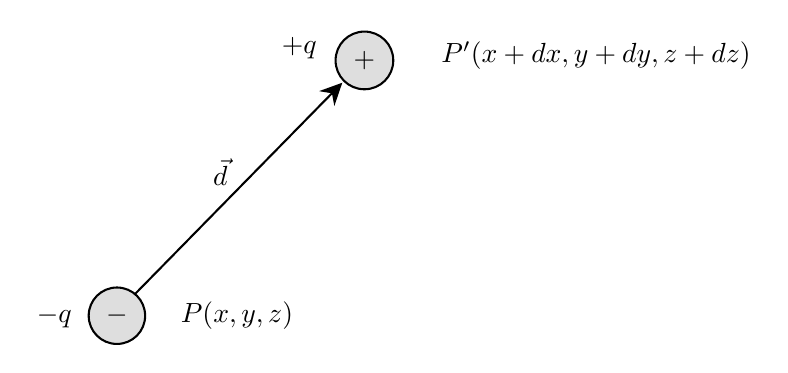
\begin{tikzpicture}[x=0.75pt,y=0.75pt,yscale=-1,xscale=1]
	%uncomment if require: \path (0,300); %set diagram left start at 0, and has height of 300

	%Straight Lines [id:da8155935001916037] 
	\draw    (253.33,181.44) -- (351.23,81.64) ;
	\draw [shift={(353.33,79.5)}, rotate = 494.45] [fill={rgb, 255:red, 0; green, 0; blue, 0 }  ][line width=0.08]  [draw opacity=0] (10.72,-5.15) -- (0,0) -- (10.72,5.15) -- (7.12,0) -- cycle    ;

	% Text Node
	\draw  [fill={rgb, 255:red, 222; green, 222; blue, 222 }  ,fill opacity=1 ]  (244.75, 191.75) circle [x radius= 13.6, y radius= 13.6]   ;
	\draw (244.75,191.75) node    {$-$};
	% Text Node
	\draw  [fill={rgb, 255:red, 222; green, 222; blue, 222 }  ,fill opacity=1 ]  (364, 68.75) circle [x radius= 13.9, y radius= 13.9]   ;
	\draw (364,68.75) node    {$+$};
	% Text Node
	\draw (294.6,122.6) node    {$\vec{d}$};
	% Text Node
	\draw (475.6,66.6) node    {$P'( x+dx,y+dy,z+dz)$};
	% Text Node
	\draw (302.6,191.6) node    {$P( x,y,z)$};
	% Text Node
	\draw (214.6,192.6) node    {$-q$};
	% Text Node
	\draw (332.6,62.6) node    {$+q$};

	\end{tikzpicture}
\end{figure}
\FloatBarrier

L'energia elettrostatica di un dipolo immerso in un campo elettrico:

\begin{align*}
	U_e &= qV(P') - qV(P) = q \left[ V(P')-V(P) \right] = q\,dV \\
	&= q\left[ \vec{\nabla} V \cdot \vec{d}  \right] =\vec{\nabla} V \cdot q\vec{d} =\vec{\nabla} V \cdot \vec{p} = \vec{p} \cdot \vec{\nabla} V = - \vec{p} \cdot \vec{E}
\end{align*}

Possiamo usare ragionamenti energetici per calcolare la risultante delle forze $\vec{R}$. Il lavoro compiuto da essa per spostare il dipolo di un tratto infinitesimo $d\vec{r}$ sarà pari a:

\[
	d\mathcal{L} = \vec{R} \cdot d\vec{r}
\]

Se c'è un lavoro positivo avremo una diminuzione dell'energia potenziale. Essendo infatti il campo conservativo, l'energia per compierlo viene sottratta da quella elettrostatica.

\begin{align*}
	d\mathcal{L} &= -dU_e \tag*{conservatività del campo}\\
		&= - \vec{\nabla} U_e \cdot d\vec{r}  \tag*{teorema del differenziale totale}  \\
		&= - \vec{\nabla} (- \vec{p} \cdot \vec{E}) \cdot d\vec{r} \tag*{risultato ottenuto prima} \\
		&= \vec{\nabla} (\vec{p} \cdot \vec{E}) \cdot d\vec{r} \\
		d\mathcal{L} &= \vec{R} \cdot d\vec{r} \tag*{definizione di lavoro}
\end{align*}

\begin{gather*}
	\implies \boxed{\vec{R} = \vec{\nabla} (\vec{p} \cdot \vec{E})} \quad \text{per campi conservativi} \\
	\boxed{\vec{R} = (\vec{p} \cdot \vec{\nabla} )\vec{E}} \quad \text{per tutti i campi}
\end{gather*}

Questo risultato (il primo) significa che il dipolo, una volta allineato, tende a portarsi nei punti in cui il campo è più intenso se il momento $\vec{p}$ è concorde al campo, mentre ad allontanarsene se $\vec{p}$ è discorde al campo.

\section{I conduttori}

Il conduttore è un qualunque materiale caratterizzato dal fatto che al suo interno sono verificate particolari condizioni per cui è possibile il moto di alcune delle cariche che lo costituiscono. Un esempio di conduzione è ciò che accade ad esempio in una soluzione salina all'interno di una cella elettrolitica, in cui si osserva un moto ambipolare di ioni (entrambe le polarità si muovono). Questo corso tuttavia si limita allo studio di conduttori allo stato solido, che generalmente sono di carattere metallico. Solitamente in un conduttore metallico ogni atomo mette in compartecipazione con l'intero sistema uno dei suoi elettroni o più. Questa situazione può essere schematizzata come un gas di elettroni libero di muoversi all'interno del materiale. Se esso è imperturbato, ossia se non agisce un campo elettrico esterno, le cariche si muovono, come in un gas, di moto puramente caotico. Quando parliamo di campo elettrico del materiale non ci occupiamo del campo elettrico microscopico. Se lo facessimo infatti basterebbe spostarsi di un solo angstrom per avere delle perturbazioni enormi su scala spaziale. Tali perturbazioni avvengono anche su scala temporale, perché l'elettrone sta orbitando quindi quando esso si sposta il campo elettrico cambia. Non possiamo quindi studiare le proprietà elettriche su scala realmente microscopica ma introdurremo le varie grandezze su scala media. Ad esempio considereremo il campo elettrico medio presente in un cubetto microscopico (in cui ho comunque un numero molto elevato di atomi). Questo vale per il campo elettrico così come per altre considerazioni. Lo stesso approccio infatti ci porta anche a dire che la velocità vettoriale media delle particelle è pari a zero. Questo perché in un conduttore non sottoposto a campi elettrici, per ogni elettrone che si muove verso il basso ce ne sarà uno che si muove verso l'alto. Quando parliamo di tutte queste quantità, stiamo parlando di grandezze mediate su scale sufficientemente grandi ma sufficientemente piccole dal punto di vista macroscopico.

\section{Conduttori in equilibrio elettrostatico}

Ci occuperemo in particolare di conduttori in equilibrio elettrostatico. Questo significa che se consideriamo un oggetto composto da materiale conduttore e vi deponiamo una carica, assumeremo che essa si distribuisca su di esso, ma attenderemo un tempo sufficientemente lungo per permettere al sistema di raggiungere una situazione stazionaria. Le cariche così saranno all'equilibrio compensando perfettamente tutte le forze di interazione fra di loro.
Nei conduttori sono gli elettroni a muoversi. Se vogliamo quindi caricare positivamente un oggetto quello che dobbiamo fare è andare a sottrarre degli elettroni. Siccome utilizzare questa logica risulta più contorto, quello che facciamo è di immaginare che sia possibile caricare un conduttore sia aggiungendo cariche positive che negative. Si tratta di una convenzione che non cambia nulla dal punto di vista concettuale.

\paragraph{Proprietà dei conduttori.} Supponiamo di aver caricato un conduttore. Nel momento in cui viene raggiunto l'equilibrio elettrostatico, il campo elettrico all'interno di tale conduttore è nullo. Esso contiene al suo interno un'enorme quantità di cariche libere di muoversi. Se $\vec{E} $ fosse diverso da zero, agirebbe una forza coulombiana che farebbe spostare le cariche, esse nel nostro caso però sono ferme. Questa è la proprietà fondamentale da cui deriveranno tutte le altre proprietà.
Ora consideriamo un punto $P$ qualsiasi all'interno del nostro conduttore. Ivi il campo elettrico, per quanto appena detto, è pari a zero e allo stesso tempo la prima equazione di Maxwell deve essere verificata:

\[
	\text{div}\vec{E} (P)=\frac{\rho (P)}{\varepsilon_0} = 0 \implies \rho (P)=0
\]

Troviamo che la densità di carica in tale punto deve essere nulla. Questo potrebbe sembrare un paradosso. Tuttavia tale densità deve essere interpretata in modo fisico come densità di carica netta. Questo significa che se consideriamo un cubettino piccolissimo, di dimensioni infinitesime, la somma delle cariche elettriche in quel punto è zero, ma non vuol dire che queste non siano presenti. Il numero di cariche positive è pari al numero di cariche negative: in ogni punto del conduttore c'è un bilanciamento perfetto fra $+$ e $-$. Se aggiungiamo della carica ad un conduttore essa non può andare a finire all'interno, l'unico punti in cui si può distribuire è la superficie. A questo punto consideriamo un percorso $ \gamma  $ che congiunge due punti all'interno del conduttore $P$ e $P'$. Possiamo osservare che, ricordando il fatto che $\vec{E} $ è nullo all'equilibrio:

\[
	V(P)-V(P') = \int_{\gamma}\vec{E} \cdot d\vec{l} =0 \implies V(P') = V(P)
\]

\begin{figure}[htpb]
	\centering

	% Pattern Info
	 
	\tikzset{
	pattern size/.store in=\mcSize, 
	pattern size = 5pt,
	pattern thickness/.store in=\mcThickness, 
	pattern thickness = 0.3pt,
	pattern radius/.store in=\mcRadius, 
	pattern radius = 1pt}
	\makeatletter
	\pgfutil@ifundefined{pgf@pattern@name@_axll6w49l}{
	\pgfdeclarepatternformonly[\mcThickness,\mcSize]{_axll6w49l}
	{\pgfqpoint{0pt}{0pt}}
	{\pgfpoint{\mcSize+\mcThickness}{\mcSize+\mcThickness}}
	{\pgfpoint{\mcSize}{\mcSize}}
	{
	\pgfsetcolor{\tikz@pattern@color}
	\pgfsetlinewidth{\mcThickness}
	\pgfpathmoveto{\pgfqpoint{0pt}{0pt}}
	\pgfpathlineto{\pgfpoint{\mcSize+\mcThickness}{\mcSize+\mcThickness}}
	\pgfusepath{stroke}
	}}
	\makeatother
	\tikzset{every picture/.style={line width=0.75pt}} %set default line width to 0.75pt        

	\begin{tikzpicture}[x=0.75pt,y=0.75pt,yscale=-1,xscale=1]
	%uncomment if require: \path (0,300); %set diagram left start at 0, and has height of 300

	%Shape: Circle [id:dp18105265613022237] 
	\draw  [pattern=_axll6w49l,pattern size=6pt,pattern thickness=0.75pt,pattern radius=0pt, pattern color={rgb, 255:red, 222; green, 222; blue, 222}] (192,145.25) .. controls (192,90.44) and (236.44,46) .. (291.25,46) .. controls (346.06,46) and (390.5,90.44) .. (390.5,145.25) .. controls (390.5,200.06) and (346.06,244.5) .. (291.25,244.5) .. controls (236.44,244.5) and (192,200.06) .. (192,145.25) -- cycle ;
	%Curve Lines [id:da6091614584116016] 
	\draw    (247,141) .. controls (268.5,100) and (322.5,199) .. (347,141) ;
	%Shape: Circle [id:dp1808319466488788] 
	\draw  [fill={rgb, 255:red, 0; green, 0; blue, 0 }  ,fill opacity=1 ] (245.14,141) .. controls (245.14,139.97) and (245.97,139.14) .. (247,139.14) .. controls (248.03,139.14) and (248.86,139.97) .. (248.86,141) .. controls (248.86,142.03) and (248.03,142.86) .. (247,142.86) .. controls (245.97,142.86) and (245.14,142.03) .. (245.14,141) -- cycle ;
	%Shape: Circle [id:dp4526096831203399] 
	\draw  [fill={rgb, 255:red, 0; green, 0; blue, 0 }  ,fill opacity=1 ] (345.14,141) .. controls (345.14,139.97) and (345.97,139.14) .. (347,139.14) .. controls (348.03,139.14) and (348.86,139.97) .. (348.86,141) .. controls (348.86,142.03) and (348.03,142.86) .. (347,142.86) .. controls (345.97,142.86) and (345.14,142.03) .. (345.14,141) -- cycle ;

	% Text Node
	\draw (291.25,36) node    {$+$};
	% Text Node
	\draw (291.25,256) node    {$+$};
	% Text Node
	\draw (401.25,146) node    {$+$};
	% Text Node
	\draw (181.25,146) node    {$+$};
	% Text Node
	\draw (369.03,68.22) node    {$+$};
	% Text Node
	\draw (213.47,223.78) node    {$+$};
	% Text Node
	\draw (369.03,223.78) node    {$+$};
	% Text Node
	\draw (213.47,68.22) node    {$+$};
	% Text Node
	\draw (334.23,44.74) node    {$+$};
	% Text Node
	\draw (248.27,247.26) node    {$+$};
	% Text Node
	\draw (392.51,188.98) node    {$+$};
	% Text Node
	\draw (189.99,103.02) node    {$+$};
	% Text Node
	\draw (393.24,104.79) node    {$+$};
	% Text Node
	\draw (189.26,187.21) node    {$+$};
	% Text Node
	\draw (332.46,247.99) node    {$+$};
	% Text Node
	\draw (250.04,44.01) node    {$+$};
	% Text Node
	\draw (238.57,150.73) node    {$P$};
	% Text Node
	\draw (359.42,134.73) node    {$P'$};
	% Text Node
	\draw (305.99,135.31) node    {$\gamma $};

	\end{tikzpicture}
\end{figure}
\FloatBarrier

Ciò significa che \textbf{il conduttore è equipotenziale}, tutti i punti al suo interno lo sono. Il risultato varrebbe anche se il punto $P'$ stesse sulla superficie. Se chiamiamo $ \Sigma  $ una superficie al suo interno, sarà sempre tale.

\section{Il teorema di Coulomb}

Applichiamo ora le condizioni al contorno anche al conduttore, per legare i valori che assume all'interno con quelli che ha all'esterno. Chiamiamo $1$ la regione del vuoto che circonda il conduttore e $2$ quella del conduttore stesso. Come abbiamo visto in precedenza, possiamo legare fra di loro i valori dei campi elettrici in prossimità di un punto sulla superficie di separazione da un lato e dall'altro. Chiamiamoli rispettivamente $\vec{E}_1$ ed $\vec{E}_2$.

\begin{align*}
	E_{1t} &= \vec{E}_1\cdot \vec{u}_t \\
	E_{2t} &= \vec{E}_2\cdot \vec{u}_t = 0\\
\end{align*}

Ci aspettiamo che il campo elettrico $\vec{E}_1$ sulla superficie sia perpendicolare ad essa. Se esso avesse una componente tangente infatti le cariche presenti sulla superficie comincerebbero a circolare. Inoltre tale superficie è equipotenziale, ed essendo $ \vec{E} = -\text{grad}V $, il campo elettrico deve essere perpendicolare ad essa. Introduciamo poi una normale $n$ alla superficie e le componenti normali:

\begin{align*}
	E_{1n} &= \vec{E}_1\cdot \vec{n} \\
	E_{2n} &= \vec{E}_2\cdot \vec{n} = 0
\end{align*}

Applicando la condizione al contorno otteniamo che:

\[
	E_{1n} - \underbrace{E_{2n}}_{=0} = \frac{\sigma}{\varepsilon_0}  \implies \boxed{\vec{E}_1 = \frac{\sigma}{\varepsilon_0}\vec{n}}
\]

Questo risultato prende il nome di \textbf{teorema di Coulomb}.

\begin{figure}[htpb]
	\centering

	% Pattern Info
	 
	\tikzset{
	pattern size/.store in=\mcSize, 
	pattern size = 5pt,
	pattern thickness/.store in=\mcThickness, 
	pattern thickness = 0.3pt,
	pattern radius/.store in=\mcRadius, 
	pattern radius = 1pt}
	\makeatletter
	\pgfutil@ifundefined{pgf@pattern@name@_mrblqmza0}{
	\pgfdeclarepatternformonly[\mcThickness,\mcSize]{_mrblqmza0}
	{\pgfqpoint{0pt}{0pt}}
	{\pgfpoint{\mcSize+\mcThickness}{\mcSize+\mcThickness}}
	{\pgfpoint{\mcSize}{\mcSize}}
	{
	\pgfsetcolor{\tikz@pattern@color}
	\pgfsetlinewidth{\mcThickness}
	\pgfpathmoveto{\pgfqpoint{0pt}{0pt}}
	\pgfpathlineto{\pgfpoint{\mcSize+\mcThickness}{\mcSize+\mcThickness}}
	\pgfusepath{stroke}
	}}
	\makeatother
	\tikzset{every picture/.style={line width=0.75pt}} %set default line width to 0.75pt        

	\begin{tikzpicture}[x=0.75pt,y=0.75pt,yscale=-1,xscale=1]
	%uncomment if require: \path (0,300); %set diagram left start at 0, and has height of 300

	%Shape: Circle [id:dp3658297706442104] 
	\draw  [pattern=_mrblqmza0,pattern size=6pt,pattern thickness=0.75pt,pattern radius=0pt, pattern color={rgb, 255:red, 222; green, 222; blue, 222}] (212,165.25) .. controls (212,110.44) and (256.44,66) .. (311.25,66) .. controls (366.06,66) and (410.5,110.44) .. (410.5,165.25) .. controls (410.5,220.06) and (366.06,264.5) .. (311.25,264.5) .. controls (256.44,264.5) and (212,220.06) .. (212,165.25) -- cycle ;
	%Straight Lines [id:da9128998526785432] 
	\draw    (396,113.67) -- (341.97,30.52) ;
	\draw [shift={(340.33,28)}, rotate = 416.98] [fill={rgb, 255:red, 0; green, 0; blue, 0 }  ][line width=0.08]  [draw opacity=0] (10.72,-5.15) -- (0,0) -- (10.72,5.15) -- (7.12,0) -- cycle    ;
	%Straight Lines [id:da35503145261724756] 
	\draw    (396,113.67) -- (479.15,59.63) ;
	\draw [shift={(481.67,58)}, rotate = 506.98] [fill={rgb, 255:red, 0; green, 0; blue, 0 }  ][line width=0.08]  [draw opacity=0] (10.72,-5.15) -- (0,0) -- (10.72,5.15) -- (7.12,0) -- cycle    ;
	%Straight Lines [id:da4195765778648737] 
	\draw    (394,110.67) -- (437.32,82.52) ;
	\draw [shift={(439.83,80.88)}, rotate = 506.98] [fill={rgb, 255:red, 0; green, 0; blue, 0 }  ][line width=0.08]  [draw opacity=0] (10.72,-5.15) -- (0,0) -- (10.72,5.15) -- (7.12,0) -- cycle    ;

	% Text Node
	\draw (311.25,56) node    {$+$};
	% Text Node
	\draw (311.25,276) node    {$+$};
	% Text Node
	\draw (421.25,166) node    {$+$};
	% Text Node
	\draw (201.25,166) node    {$+$};
	% Text Node
	\draw (389.03,88.22) node    {$+$};
	% Text Node
	\draw (233.47,243.78) node    {$+$};
	% Text Node
	\draw (389.03,243.78) node    {$+$};
	% Text Node
	\draw (233.47,88.22) node    {$+$};
	% Text Node
	\draw (354.23,64.74) node    {$+$};
	% Text Node
	\draw (268.27,267.26) node    {$+$};
	% Text Node
	\draw (412.51,208.98) node    {$+$};
	% Text Node
	\draw (209.99,123.02) node    {$+$};
	% Text Node
	\draw (413.24,124.79) node    {$+$};
	% Text Node
	\draw (209.26,207.21) node    {$+$};
	% Text Node
	\draw (352.46,267.99) node    {$+$};
	% Text Node
	\draw (270.04,64.01) node    {$+$};
	% Text Node
	\draw (365.56,37.41) node    {$\vec{u}_{t}$};
	% Text Node
	\draw (495.56,66.08) node    {$\vec{u}_{n}$};
	% Text Node
	\draw (413.56,75.41) node    {$\vec{E}_{1}$};
	% Text Node
	\draw (311.25,165.25) node    {$\vec{E}_{2} =0$};

	\end{tikzpicture}
\end{figure}
\FloatBarrier

Una volta notato il fatto che la superficie esterna è equipotenziale, c'è un altra condizione che permette di dimostrare subito che il potenziale è costante anche dentro il conduttore. Infatti, se consideriamo ancora una volta il nostro conduttore carico, possiamo ricorrere all'equazione di Poisson:

\[
	\nabla^2 V = -\frac{\rho}{\varepsilon_0} = 0 \implies \nabla^2 V = 0\quad \text{sul conduttore}
\]

Ottenendo così l'equazione omogenea associata, che abbiamo visto essere l'equazione di Laplace. A questo punto ricordiamo che il teorema della media afferma che una funzione che soddisfa l'equazione di Laplace non ha né punti di minimo né di massimo. Ma siccome stiamo già vincolando il potenziale ad essere costante sulla superficie, deve essere costante anche in tutti gli altri punti del conduttore. La funzione potenziale è un equazione armonica, ecco perché il conduttore è equipotenziale non solo sulla superficie ma anche all'interno.

\section{Il potere delle punte}

Immaginiamo di considerare due conduttori sferici: uno di raggio $R_1 $ e uno un po' più piccolo di raggio $R_2<R_1$. Poniamo di collegarli con un filo conduttore e assumiamo che tale filo abbia una quantità di carica trascurabile.

In questo modo si viene a costituire un unico corpo conduttore e in equilibrio vale ovunque la condizione $\vec{E}=0 $, $V=\text{costante}$: i conduttori a contatto hanno lo stesso potenziale. Inoltre poniamo che i conduttori siano molto lontani fra di loro, di modo tale che non si influenzino l'un con l'altro tramite i campi elettrici: sono praticamente isolati. Siccome tutto il sistema è conduttore, tutti i conduttori sono allo stesso potenziale. Chiamiamo $V_1$ il potenziale del conduttore più grande e $V_2$ quello di quello più piccolo.

\begin{figure}[htpb]
	\centering

	% Pattern Info
	 
	\tikzset{
	pattern size/.store in=\mcSize, 
	pattern size = 5pt,
	pattern thickness/.store in=\mcThickness, 
	pattern thickness = 0.3pt,
	pattern radius/.store in=\mcRadius, 
	pattern radius = 1pt}
	\makeatletter
	\pgfutil@ifundefined{pgf@pattern@name@_zaytzot61}{
	\pgfdeclarepatternformonly[\mcThickness,\mcSize]{_zaytzot61}
	{\pgfqpoint{0pt}{0pt}}
	{\pgfpoint{\mcSize+\mcThickness}{\mcSize+\mcThickness}}
	{\pgfpoint{\mcSize}{\mcSize}}
	{
	\pgfsetcolor{\tikz@pattern@color}
	\pgfsetlinewidth{\mcThickness}
	\pgfpathmoveto{\pgfqpoint{0pt}{0pt}}
	\pgfpathlineto{\pgfpoint{\mcSize+\mcThickness}{\mcSize+\mcThickness}}
	\pgfusepath{stroke}
	}}
	\makeatother

	% Pattern Info
	 
	\tikzset{
	pattern size/.store in=\mcSize, 
	pattern size = 5pt,
	pattern thickness/.store in=\mcThickness, 
	pattern thickness = 0.3pt,
	pattern radius/.store in=\mcRadius, 
	pattern radius = 1pt}
	\makeatletter
	\pgfutil@ifundefined{pgf@pattern@name@_sxfafmyuk}{
	\pgfdeclarepatternformonly[\mcThickness,\mcSize]{_sxfafmyuk}
	{\pgfqpoint{0pt}{0pt}}
	{\pgfpoint{\mcSize+\mcThickness}{\mcSize+\mcThickness}}
	{\pgfpoint{\mcSize}{\mcSize}}
	{
	\pgfsetcolor{\tikz@pattern@color}
	\pgfsetlinewidth{\mcThickness}
	\pgfpathmoveto{\pgfqpoint{0pt}{0pt}}
	\pgfpathlineto{\pgfpoint{\mcSize+\mcThickness}{\mcSize+\mcThickness}}
	\pgfusepath{stroke}
	}}
	\makeatother
	\tikzset{every picture/.style={line width=0.75pt}} %set default line width to 0.75pt        

	\begin{tikzpicture}[x=0.75pt,y=0.75pt,yscale=-0.8,xscale=0.8]
	%uncomment if require: \path (0,300); %set diagram left start at 0, and has height of 300

	%Shape: Circle [id:dp628173292640839] 
	\draw  [pattern=_zaytzot61,pattern size=6pt,pattern thickness=0.75pt,pattern radius=0pt, pattern color={rgb, 255:red, 222; green, 222; blue, 222}] (75,144.25) .. controls (75,89.44) and (119.44,45) .. (174.25,45) .. controls (229.06,45) and (273.5,89.44) .. (273.5,144.25) .. controls (273.5,199.06) and (229.06,243.5) .. (174.25,243.5) .. controls (119.44,243.5) and (75,199.06) .. (75,144.25) -- cycle ;
	%Straight Lines [id:da5492081302142064] 
	\draw    (174.25,144.25) -- (174.25,45) ;
	%Shape: Ellipse [id:dp9195499353482499] 
	\draw  [pattern=_sxfafmyuk,pattern size=6pt,pattern thickness=0.75pt,pattern radius=0pt, pattern color={rgb, 255:red, 222; green, 222; blue, 222}] (448.57,141.56) .. controls (448.57,112.03) and (472.5,88.09) .. (502.03,88.09) .. controls (531.56,88.09) and (555.5,112.03) .. (555.5,141.56) .. controls (555.5,171.09) and (531.56,195.02) .. (502.03,195.02) .. controls (472.5,195.02) and (448.57,171.09) .. (448.57,141.56) -- cycle ;
	%Straight Lines [id:da08931752397680315] 
	\draw    (502.03,140.56) -- (502.03,82.09) ;
	%Curve Lines [id:da21347577099567938] 
	\draw [line width=2.25]    (273.5,144.25) .. controls (336.5,57) and (398.5,229) .. (448.57,141.56) ;

	% Text Node
	\draw (174.25,35) node    {$+$};
	% Text Node
	\draw (174.25,255) node    {$+$};
	% Text Node
	\draw (284.25,145) node    {$+$};
	% Text Node
	\draw (64.25,145) node    {$+$};
	% Text Node
	\draw (252.03,67.22) node    {$+$};
	% Text Node
	\draw (96.47,222.78) node    {$+$};
	% Text Node
	\draw (252.03,222.78) node    {$+$};
	% Text Node
	\draw (96.47,67.22) node    {$+$};
	% Text Node
	\draw (217.23,43.74) node    {$+$};
	% Text Node
	\draw (131.27,246.26) node    {$+$};
	% Text Node
	\draw (275.51,187.98) node    {$+$};
	% Text Node
	\draw (72.99,102.02) node    {$+$};
	% Text Node
	\draw (276.24,103.79) node    {$+$};
	% Text Node
	\draw (72.26,186.21) node    {$+$};
	% Text Node
	\draw (215.46,246.99) node    {$+$};
	% Text Node
	\draw (133.04,43.01) node    {$+$};
	% Text Node
	\draw (189.56,98.41) node    {$R_{1}$};
	% Text Node
	\draw (269.56,41.41) node    {$Q_{1} ,V_{1}$};
	% Text Node
	\draw (502.03,76.2) node    {$+$};
	% Text Node
	\draw (502.03,205.8) node    {$+$};
	% Text Node
	\draw (566.84,141) node    {$+$};
	% Text Node
	\draw (437.23,141) node    {$+$};
	% Text Node
	\draw (547.86,95.18) node    {$+$};
	% Text Node
	\draw (456.21,186.82) node    {$+$};
	% Text Node
	\draw (547.86,186.82) node    {$+$};
	% Text Node
	\draw (456.21,95.18) node    {$+$};
	% Text Node
	\draw (527.35,81.35) node    {$+$};
	% Text Node
	\draw (476.71,200.65) node    {$+$};
	% Text Node
	\draw (561.68,166.32) node    {$+$};
	% Text Node
	\draw (442.38,115.68) node    {$+$};
	% Text Node
	\draw (562.12,116.72) node    {$+$};
	% Text Node
	\draw (441.95,165.28) node    {$+$};
	% Text Node
	\draw (526.31,201.08) node    {$+$};
	% Text Node
	\draw (477.76,80.92) node    {$+$};
	% Text Node
	\draw (516.05,113.55) node    {$R_{2}$};
	% Text Node
	\draw (576.18,77.98) node    {$Q_{2} ,V_{2}$};

	\end{tikzpicture}
\end{figure}
\FloatBarrier

Si trova che:

\begin{gather*}
	V(\infty) = 0 \qquad V_1=\frac{Q_1}{4\pi \varepsilon_0 R_1} \qquad V_2=\frac{Q_2}{4\pi \varepsilon_0 R_2} \qquad V_1=V_2 \\
	\frac{Q_1}{4\pi \varepsilon_0 R_1} = \frac{Q_2}{4\pi \varepsilon_0 R_2} \implies \frac{Q_1}{Q_2} = \frac{R_1}{R_2} \\
	\frac{\sigma_1}{\sigma_2} = \frac{\frac{Q_1}{4\pi R_1^2}}{\frac{Q_2}{4\pi R_2^2}} = \frac{Q_1}{Q_2} \frac{R_2^2}{R_1^2} = \frac{R_1}{R_2} \frac{R_2^2}{R_1^2} = \frac{R_2}{R_1} \\
	\boxed{\frac{\sigma_1}{\sigma_2} = \frac{R_2}{R_1}}
\end{gather*}

Otteniamo che la densità di carica superficiale è inversamente proporzionale al suo raggio di curvatura.

\begin{figure}[htpb]
	\centering

	\tikzset{every picture/.style={line width=0.75pt}} %set default line width to 0.75pt        

	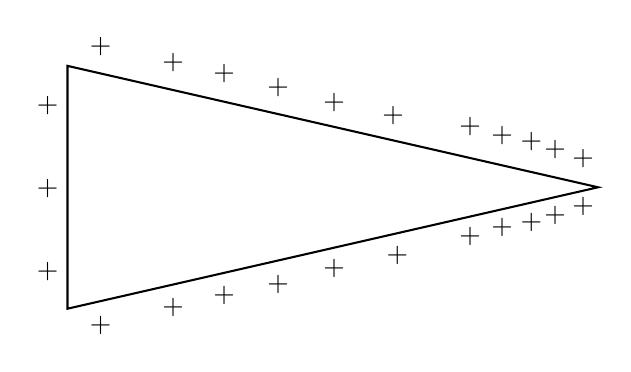
\begin{tikzpicture}[x=0.75pt,y=0.75pt,yscale=-1,xscale=1]
	%uncomment if require: \path (0,300); %set diagram left start at 0, and has height of 300

	%Shape: Triangle [id:dp6864512559833931] 
	\draw   (370.65,122.5) -- (115,181) -- (115,64) -- cycle ;

	% Text Node
	\draw (105.46,82.99) node    {$+$};
	% Text Node
	\draw (105.46,122.99) node    {$+$};
	% Text Node
	\draw (105.46,162.99) node    {$+$};
	% Text Node
	\draw (363.46,108.49) node    {$+$};
	% Text Node
	\draw (349.96,104.49) node    {$+$};
	% Text Node
	\draw (338.46,100.49) node    {$+$};
	% Text Node
	\draw (324.46,97.49) node    {$+$};
	% Text Node
	\draw (308.96,93.49) node    {$+$};
	% Text Node
	\draw (271.96,87.99) node    {$+$};
	% Text Node
	\draw (243.46,81.49) node    {$+$};
	% Text Node
	\draw (216.46,74.49) node    {$+$};
	% Text Node
	\draw (190.46,67.49) node    {$+$};
	% Text Node
	\draw (165.96,62.49) node    {$+$};
	% Text Node
	\draw (130.96,54.49) node    {$+$};
	% Text Node
	\draw (363.46,131.54) node  [rotate=-180,xscale=-1]  {$+$};
	% Text Node
	\draw (349.96,135.96) node  [rotate=-180,xscale=-1]  {$+$};
	% Text Node
	\draw (338.46,139.38) node  [rotate=-180,xscale=-1]  {$+$};
	% Text Node
	\draw (324.46,141.69) node  [rotate=-180,xscale=-1]  {$+$};
	% Text Node
	\draw (308.96,146.11) node  [rotate=-180,xscale=-1]  {$+$};
	% Text Node
	\draw (273.96,155.19) node  [rotate=-180,xscale=-1]  {$+$};
	% Text Node
	\draw (243.46,161.37) node  [rotate=-180,xscale=-1]  {$+$};
	% Text Node
	\draw (216.46,169.1) node  [rotate=-180,xscale=-1]  {$+$};
	% Text Node
	\draw (190.46,174.84) node  [rotate=-180,xscale=-1]  {$+$};
	% Text Node
	\draw (165.96,180.36) node  [rotate=-180,xscale=-1]  {$+$};
	% Text Node
	\draw (130.96,189.2) node  [rotate=-180,xscale=-1]  {$+$};

	\end{tikzpicture}
\end{figure}
\FloatBarrier

Supponiamo di avere un conduttore dalla forma appuntita come in figura. In una certa posizione, il raggio di curvatura è piccolissimo. Siccome qui accade ciò, la densità di carica è molto elevata. Ecco quindi che la carica si distribuisce in modo più fitto in prossimità della punta. In quel punto avremo un campo elettrico molto intenso. Questa proprietà prende il nome di \textbf{potere delle punte}. Sperimentalmente si osserva che se prendiamo un conduttore con una punta e lo carichiamo, in prossimità di essa avremo un campo elettrico molto intenso tale da poter ionizzare le molecole d'aria intorno ad essa. Da questo effetto hanno origine svariati fenomeni, come la formazione di scintille tra elettrodi di forma appuntita in ambiente gassoso o l'effluvio di elettroni da punte cariche negativamente, che avviene anche nel vuoto.
Il parafulmine si basa su questo principio, la punta ionizza l'aria in prossimità e il fulmine cade in quel luogo perché c'è già un percorso conduttivo pronto. Vi sono moltissime altre applicazioni pratiche di questo concetto.

\section{Conduttori cavi}

Un conduttore cavo è un conduttore che al suo interno ha una cavità vuota. Supponiamo di averne uno caricato come in figura.

Non potrebbe darsi che la carica sulla superficie attraversi la parete e si depositi sulla superficie interna?
\emph{Dimostrazione per assurdo.} Se consideriamo una superficie astratta gaussiana all'interno del conduttore e applichiamo ad essa il teorema di Gauss si ha che:

\begin{gather*}
	\Phi_{\Sigma_g}(\vec{E}) = \frac{Q_{\text{tot}}}{\varepsilon_0} = \int_{\Sigma_g} \vec{E} \cdot \vec{n} dS = 0 \implies Q_{\text{tot}} = 0
\end{gather*}

Quindi questa carica interna non può esistere perché il campo nel conduttore è nullo, e quindi anche il suo flusso attraverso la superficie $ \Sigma_g  $.

Supponiamo che per qualche motivo si formino cariche di segno opposto ai due estremi della cavità. Se il numero di cariche positive è uguale a quello di cariche negative, le condizioni riguardanti l'equilibrio elettrostatico del sistema non vengono violate. Tuttavia questa situazione non è possibile: per negare questa circostanza si ricorre alla proprietà di conservatività. Scegliamo un percorso chiuso che si ottiene come in figura.

\begin{gather*}
	\oint_{\gamma} \vec{E} \cdot d\vec{l} = 0 = \int_{\text{cavità}} \vec{E} \cdot d\vec{l}  + \underbrace{\int_{\text{conduttore}} \vec{E} \cdot d\vec{l}}_{=0} \\
	\implies \int_{\text{cavità}} \vec{E} \cdot d\vec{l} = 0
\end{gather*}

Arriviamo così ad un paradosso: la proprietà di circuitazione pari a $0$ ci dice che non ci può essere un campo elettrico all'interno della cavità. Ma allora non ci possono nemmeno essere cariche di segno opposto disposte in tal modo. Quindi è impossibile una separazione di carica sulle pareti della cavità. Qualunque sia la quantità di carica deposta sul conduttore, sulla superficie della cavità la carica elettrica va a zero. Inoltre è chiaro che il potenziale in un qualsiasi punto della cavità è uguale a quello del conduttore: se ci fosse una d.d.p. dovrebbe infatti esserci un campo diverso da $0$. In conclusione, \emph{la carica di un conduttore in equilibrio si distribuisce sempre e soltanto sulla superficie esterna, anche se il conduttore è cavo}.
È come se la cavità non risentisse dei fenomeni elettrostatici che avvengono al di fuori. Un'oggetto del genere viene chiamato \textbf{schermo elettrostatico}, tutto si arresta alla superficie, non penetra nel conduttore. Quando vogliamo proteggere un oggetto da fenomeni elettrostatici, basta circondarlo con un materiale conduttore. La gabbia metallica, chiamata anche \emph{gabbia di Faraday}, si basa proprio su questo principio ed è un modo per protegger qualcosa da disturbi elettromagnetici.

\begin{figure}[htpb]
	\centering

	% Pattern Info
	 
	\tikzset{
	pattern size/.store in=\mcSize, 
	pattern size = 5pt,
	pattern thickness/.store in=\mcThickness, 
	pattern thickness = 0.3pt,
	pattern radius/.store in=\mcRadius, 
	pattern radius = 1pt}
	\makeatletter
	\pgfutil@ifundefined{pgf@pattern@name@_n77hebug6}{
	\pgfdeclarepatternformonly[\mcThickness,\mcSize]{_n77hebug6}
	{\pgfqpoint{0pt}{0pt}}
	{\pgfpoint{\mcSize+\mcThickness}{\mcSize+\mcThickness}}
	{\pgfpoint{\mcSize}{\mcSize}}
	{
	\pgfsetcolor{\tikz@pattern@color}
	\pgfsetlinewidth{\mcThickness}
	\pgfpathmoveto{\pgfqpoint{0pt}{0pt}}
	\pgfpathlineto{\pgfpoint{\mcSize+\mcThickness}{\mcSize+\mcThickness}}
	\pgfusepath{stroke}
	}}
	\makeatother

	% Pattern Info
	 
	\tikzset{
	pattern size/.store in=\mcSize, 
	pattern size = 5pt,
	pattern thickness/.store in=\mcThickness, 
	pattern thickness = 0.3pt,
	pattern radius/.store in=\mcRadius, 
	pattern radius = 1pt}
	\makeatletter
	\pgfutil@ifundefined{pgf@pattern@name@_ly2th85di}{
	\pgfdeclarepatternformonly[\mcThickness,\mcSize]{_ly2th85di}
	{\pgfqpoint{0pt}{0pt}}
	{\pgfpoint{\mcSize+\mcThickness}{\mcSize+\mcThickness}}
	{\pgfpoint{\mcSize}{\mcSize}}
	{
	\pgfsetcolor{\tikz@pattern@color}
	\pgfsetlinewidth{\mcThickness}
	\pgfpathmoveto{\pgfqpoint{0pt}{0pt}}
	\pgfpathlineto{\pgfpoint{\mcSize+\mcThickness}{\mcSize+\mcThickness}}
	\pgfusepath{stroke}
	}}
	\makeatother

	% Pattern Info
	 
	\tikzset{
	pattern size/.store in=\mcSize, 
	pattern size = 5pt,
	pattern thickness/.store in=\mcThickness, 
	pattern thickness = 0.3pt,
	pattern radius/.store in=\mcRadius, 
	pattern radius = 1pt}
	\makeatletter
	\pgfutil@ifundefined{pgf@pattern@name@_1wjb81hf8}{
	\pgfdeclarepatternformonly[\mcThickness,\mcSize]{_1wjb81hf8}
	{\pgfqpoint{0pt}{0pt}}
	{\pgfpoint{\mcSize+\mcThickness}{\mcSize+\mcThickness}}
	{\pgfpoint{\mcSize}{\mcSize}}
	{
	\pgfsetcolor{\tikz@pattern@color}
	\pgfsetlinewidth{\mcThickness}
	\pgfpathmoveto{\pgfqpoint{0pt}{0pt}}
	\pgfpathlineto{\pgfpoint{\mcSize+\mcThickness}{\mcSize+\mcThickness}}
	\pgfusepath{stroke}
	}}
	\makeatother
	\tikzset{every picture/.style={line width=0.75pt}} %set default line width to 0.75pt        

	\begin{tikzpicture}[x=0.75pt,y=0.75pt,yscale=-0.6,xscale=0.6]
	%uncomment if require: \path (0,352); %set diagram left start at 0, and has height of 352

	%Shape: Path Data [id:dp44392596580582233] 
	\draw  [pattern=_n77hebug6,pattern size=6pt,pattern thickness=0.75pt,pattern radius=0pt, pattern color={rgb, 255:red, 222; green, 222; blue, 222}] (105.06,83.91) .. controls (152.78,83.91) and (191.47,122.6) .. (191.47,170.33) .. controls (191.47,218.06) and (152.78,256.75) .. (105.06,256.75) .. controls (57.33,256.75) and (18.64,218.06) .. (18.64,170.33) .. controls (18.64,122.6) and (57.33,83.91) .. (105.06,83.91) -- cycle (59.13,170.33) .. controls (59.13,195.7) and (79.69,216.26) .. (105.06,216.26) .. controls (130.42,216.26) and (150.98,195.7) .. (150.98,170.33) .. controls (150.98,144.96) and (130.42,124.4) .. (105.06,124.4) .. controls (79.69,124.4) and (59.13,144.96) .. (59.13,170.33) -- cycle ;
	%Shape: Path Data [id:dp25138489216387905] 
	\draw  [pattern=_ly2th85di,pattern size=6pt,pattern thickness=0.75pt,pattern radius=0pt, pattern color={rgb, 255:red, 222; green, 222; blue, 222}] (346.26,83.91) .. controls (393.99,83.91) and (432.68,122.6) .. (432.68,170.33) .. controls (432.68,218.06) and (393.99,256.75) .. (346.26,256.75) .. controls (298.54,256.75) and (259.85,218.06) .. (259.85,170.33) .. controls (259.85,122.6) and (298.54,83.91) .. (346.26,83.91) -- cycle (300.33,170.33) .. controls (300.33,195.7) and (320.9,216.26) .. (346.26,216.26) .. controls (371.63,216.26) and (392.19,195.7) .. (392.19,170.33) .. controls (392.19,144.96) and (371.63,124.4) .. (346.26,124.4) .. controls (320.9,124.4) and (300.33,144.96) .. (300.33,170.33) -- cycle ;
	\draw  [line width=3]  (333.2,285.26) -- (358.89,310.95)(358.89,285.26) -- (333.2,310.95) ;
	%Shape: Path Data [id:dp03545183947977337] 
	\draw  [pattern=_1wjb81hf8,pattern size=6pt,pattern thickness=0.75pt,pattern radius=0pt, pattern color={rgb, 255:red, 222; green, 222; blue, 222}] (586.26,83.91) .. controls (633.99,83.91) and (672.68,122.6) .. (672.68,170.33) .. controls (672.68,218.06) and (633.99,256.75) .. (586.26,256.75) .. controls (538.54,256.75) and (499.85,218.06) .. (499.85,170.33) .. controls (499.85,122.6) and (538.54,83.91) .. (586.26,83.91) -- cycle (540.33,170.33) .. controls (540.33,195.7) and (560.9,216.26) .. (586.26,216.26) .. controls (611.63,216.26) and (632.19,195.7) .. (632.19,170.33) .. controls (632.19,144.96) and (611.63,124.4) .. (586.26,124.4) .. controls (560.9,124.4) and (540.33,144.96) .. (540.33,170.33) -- cycle ;
	%Shape: Ellipse [id:dp7252735373705406] 
	\draw  [dash pattern={on 0.84pt off 2.51pt}] (523.79,170.55) .. controls (523.79,135.92) and (551.86,107.86) .. (586.48,107.86) .. controls (621.1,107.86) and (649.17,135.92) .. (649.17,170.55) .. controls (649.17,205.17) and (621.1,233.24) .. (586.48,233.24) .. controls (551.86,233.24) and (523.79,205.17) .. (523.79,170.55) -- cycle ;
	\draw  [line width=3]  (573.2,285.26) -- (598.89,310.95)(598.89,285.26) -- (573.2,310.95) ;
	%Shape: Ellipse [id:dp10723301414510167] 
	\draw  [dash pattern={on 0.84pt off 2.51pt}] (291.4,205.2) .. controls (291.4,191.28) and (317.01,180) .. (348.6,180) .. controls (380.19,180) and (405.8,191.28) .. (405.8,205.2) .. controls (405.8,219.12) and (380.19,230.4) .. (348.6,230.4) .. controls (317.01,230.4) and (291.4,219.12) .. (291.4,205.2) -- cycle ;
	%Straight Lines [id:da7941270572000036] 
	\draw [line width=3]    (92,303) -- (104,315) ;
	%Straight Lines [id:da5628523951031692] 
	\draw [line width=3]    (119.5,287.25) -- (104,315) ;

	% Text Node
	\draw (105.06,75.21) node    {$+$};
	% Text Node
	\draw (105.06,266.76) node    {$+$};
	% Text Node
	\draw (200.83,170.98) node    {$+$};
	% Text Node
	\draw (9.28,170.98) node    {$+$};
	% Text Node
	\draw (172.78,103.26) node    {$+$};
	% Text Node
	\draw (37.33,238.71) node    {$+$};
	% Text Node
	\draw (172.78,238.71) node    {$+$};
	% Text Node
	\draw (37.33,103.26) node    {$+$};
	% Text Node
	\draw (142.48,82.82) node    {$+$};
	% Text Node
	\draw (67.63,259.14) node    {$+$};
	% Text Node
	\draw (193.22,208.41) node    {$+$};
	% Text Node
	\draw (16.89,133.56) node    {$+$};
	% Text Node
	\draw (193.86,135.1) node    {$+$};
	% Text Node
	\draw (16.25,206.86) node    {$+$};
	% Text Node
	\draw (140.93,259.78) node    {$+$};
	% Text Node
	\draw (69.18,82.18) node    {$+$};
	% Text Node
	\draw (346.26,75.21) node    {$+$};
	% Text Node
	\draw (346.26,266.76) node    {$+$};
	% Text Node
	\draw (442.04,170.98) node    {$+$};
	% Text Node
	\draw (250.49,170.98) node    {$+$};
	% Text Node
	\draw (413.99,103.26) node    {$+$};
	% Text Node
	\draw (278.54,238.71) node    {$+$};
	% Text Node
	\draw (413.99,238.71) node    {$+$};
	% Text Node
	\draw (278.54,103.26) node    {$+$};
	% Text Node
	\draw (383.69,82.82) node    {$+$};
	% Text Node
	\draw (308.84,259.14) node    {$+$};
	% Text Node
	\draw (434.43,208.41) node    {$+$};
	% Text Node
	\draw (258.1,133.56) node    {$+$};
	% Text Node
	\draw (435.06,135.1) node    {$+$};
	% Text Node
	\draw (257.46,206.86) node    {$+$};
	% Text Node
	\draw (382.14,259.78) node    {$+$};
	% Text Node
	\draw (310.38,82.18) node    {$+$};
	% Text Node
	\draw (346.26,130.19) node    {$+$};
	% Text Node
	\draw (346.26,204.81) node    {$-$};
	% Text Node
	\draw (383.58,167.5) node    {$-$};
	% Text Node
	\draw (308.95,167.5) node    {$+$};
	% Text Node
	\draw (372.65,141.12) node    {$-$};
	% Text Node
	\draw (319.88,193.88) node    {$+$};
	% Text Node
	\draw (372.65,193.88) node    {$-$};
	% Text Node
	\draw (319.88,141.12) node    {$+$};
	% Text Node
	\draw (412.16,186.89) node    {$\gamma $};
	% Text Node
	\draw (586.26,75.21) node    {$+$};
	% Text Node
	\draw (586.26,266.76) node    {$+$};
	% Text Node
	\draw (682.04,170.98) node    {$+$};
	% Text Node
	\draw (490.49,170.98) node    {$+$};
	% Text Node
	\draw (653.99,103.26) node    {$+$};
	% Text Node
	\draw (518.54,238.71) node    {$+$};
	% Text Node
	\draw (653.99,238.71) node    {$+$};
	% Text Node
	\draw (518.54,103.26) node    {$+$};
	% Text Node
	\draw (623.69,82.82) node    {$+$};
	% Text Node
	\draw (548.84,259.14) node    {$+$};
	% Text Node
	\draw (674.43,208.41) node    {$+$};
	% Text Node
	\draw (498.1,133.56) node    {$+$};
	% Text Node
	\draw (675.06,135.1) node    {$+$};
	% Text Node
	\draw (497.46,206.86) node    {$+$};
	% Text Node
	\draw (622.14,259.78) node    {$+$};
	% Text Node
	\draw (550.38,82.18) node    {$+$};
	% Text Node
	\draw (586.26,130.19) node    {$+$};
	% Text Node
	\draw (586.26,204.81) node    {$+$};
	% Text Node
	\draw (623.58,167.5) node    {$+$};
	% Text Node
	\draw (548.95,167.5) node    {$+$};
	% Text Node
	\draw (612.65,141.12) node    {$+$};
	% Text Node
	\draw (559.88,193.88) node    {$+$};
	% Text Node
	\draw (612.65,193.88) node    {$+$};
	% Text Node
	\draw (559.88,141.12) node    {$+$};
	% Text Node
	\draw (578.16,98.89) node    {$\Sigma $};

	\end{tikzpicture}
\end{figure}
\FloatBarrier

Questa proprietà funziona anche nell'altro senso. Lo schermo elettrostatico infatti scherma anche quello che accade nella cavità dall'esterno. Poniamo di essere in grado di portare all'interno della cavità una carica positiva $Q$. Chiamiamo $Q_1$ la quantità di carica che si forma sulla superficie della cavità. Sulla superficie all'esterno si distribuirà allora una carica positiva per permettere di mantenere l'equilibrio elettrostatico (la somma delle cariche è sempre la stessa). Scegliamo una superficie astratta gaussiana completamente contenuta nel conduttore e applichiamo il teorema di Gauss.

\begin{gather*}
	\left. \begin{array}{r}
	  	\Phi_{\Sigma_g}(\vec{E} ) = \frac{Q_{\text{tot}}}{\varepsilon_0} = \frac{Q+Q_1}{\varepsilon_0} \\
		\Phi_{\Sigma_g}(\vec{E} ) = \int_{\Sigma_g}\vec{E} \cdot \vec{n} dS = 0
	 \end{array} \right\} \implies Q + Q_1 = 0 \\
	 Q_1 = -Q \qquad Q_2 = -Q_1 = -(-Q) = Q
\end{gather*}

La carica puntiforme più grande, \emph{conducente}, ha indotto una carica negativa uguale al suo opposto sulla superficie interna e automaticamente una carica positiva esattamente pari in modulo sulla superficie esterna. Quando la carica elettrica indotta sulla superficie di un conduttore è esattamente opposta alla carica inducente, si parla di \textbf{induzione elettrostatica completa}.

\begin{figure}[htpb]
	\centering

	% Pattern Info
	 
	\tikzset{
	pattern size/.store in=\mcSize, 
	pattern size = 5pt,
	pattern thickness/.store in=\mcThickness, 
	pattern thickness = 0.3pt,
	pattern radius/.store in=\mcRadius, 
	pattern radius = 1pt}
	\makeatletter
	\pgfutil@ifundefined{pgf@pattern@name@_40ui31n0d}{
	\pgfdeclarepatternformonly[\mcThickness,\mcSize]{_40ui31n0d}
	{\pgfqpoint{0pt}{0pt}}
	{\pgfpoint{\mcSize+\mcThickness}{\mcSize+\mcThickness}}
	{\pgfpoint{\mcSize}{\mcSize}}
	{
	\pgfsetcolor{\tikz@pattern@color}
	\pgfsetlinewidth{\mcThickness}
	\pgfpathmoveto{\pgfqpoint{0pt}{0pt}}
	\pgfpathlineto{\pgfpoint{\mcSize+\mcThickness}{\mcSize+\mcThickness}}
	\pgfusepath{stroke}
	}}
	\makeatother
	\tikzset{every picture/.style={line width=0.75pt}} %set default line width to 0.75pt        

	\begin{tikzpicture}[x=0.75pt,y=0.75pt,yscale=-0.8,xscale=0.8]
	%uncomment if require: \path (0,384); %set diagram left start at 0, and has height of 384

	%Shape: Path Data [id:dp9078267867868894] 
	\draw  [pattern=_40ui31n0d,pattern size=6pt,pattern thickness=0.75pt,pattern radius=0pt, pattern color={rgb, 255:red, 222; green, 222; blue, 222}] (309.64,72.54) .. controls (374.27,72.54) and (426.67,124.94) .. (426.67,189.57) .. controls (426.67,254.2) and (374.27,306.6) .. (309.64,306.6) .. controls (245.01,306.6) and (192.61,254.2) .. (192.61,189.57) .. controls (192.61,124.94) and (245.01,72.54) .. (309.64,72.54) -- cycle (247.44,189.57) .. controls (247.44,223.92) and (275.29,251.77) .. (309.64,251.77) .. controls (343.99,251.77) and (371.84,223.92) .. (371.84,189.57) .. controls (371.84,155.22) and (343.99,127.37) .. (309.64,127.37) .. controls (275.29,127.37) and (247.44,155.22) .. (247.44,189.57) -- cycle ;
	%Shape: Ellipse [id:dp18926462592798] 
	\draw  [dash pattern={on 0.84pt off 2.51pt}] (217.46,188.99) .. controls (217.46,138.16) and (258.66,96.97) .. (309.48,96.97) .. controls (360.3,96.97) and (401.5,138.16) .. (401.5,188.99) .. controls (401.5,239.81) and (360.3,281) .. (309.48,281) .. controls (258.66,281) and (217.46,239.81) .. (217.46,188.99) -- cycle ;

	% Text Node
	\draw (309.64,60.75) node    {$+$};
	% Text Node
	\draw (309.64,320.16) node    {$+$};
	% Text Node
	\draw (439.34,190.45) node    {$+$};
	% Text Node
	\draw (179.94,190.45) node    {$+$};
	% Text Node
	\draw (401.35,98.74) node    {$+$};
	% Text Node
	\draw (217.93,282.17) node    {$+$};
	% Text Node
	\draw (401.35,282.17) node    {$+$};
	% Text Node
	\draw (217.93,98.74) node    {$+$};
	% Text Node
	\draw (360.32,71.06) node    {$+$};
	% Text Node
	\draw (258.96,309.84) node    {$+$};
	% Text Node
	\draw (429.03,241.13) node    {$+$};
	% Text Node
	\draw (190.25,139.77) node    {$+$};
	% Text Node
	\draw (429.9,141.86) node    {$+$};
	% Text Node
	\draw (189.38,239.04) node    {$+$};
	% Text Node
	\draw (358.23,310.71) node    {$+$};
	% Text Node
	\draw (261.05,70.19) node    {$+$};
	% Text Node
	\draw  [fill={rgb, 255:red, 222; green, 222; blue, 222 }  ,fill opacity=1 ]  (310, 188.75) circle [x radius= 13.9, y radius= 13.9]   ;
	\draw (310,188.75) node    {$+$};
	% Text Node
	\draw (329.15,141.5) node    {$-$};
	% Text Node
	\draw (290.13,233.4) node    {$-$};
	% Text Node
	\draw (355.59,206.96) node    {$-$};
	% Text Node
	\draw (263.69,167.95) node    {$-$};
	% Text Node
	\draw (355.93,168.75) node    {$-$};
	% Text Node
	\draw (263.35,206.15) node    {$-$};
	% Text Node
	\draw (328.34,233.74) node    {$-$};
	% Text Node
	\draw (290.94,141.17) node    {$-$};
	% Text Node
	\draw (334.44,185.17) node    {$Q$};
	% Text Node
	\draw (360.94,134.17) node    {$Q_{1}$};
	% Text Node
	\draw (420.94,116.67) node    {$Q_{2}$};
	% Text Node
	\draw (297.27,83.8) node    {$\Sigma $};

	\end{tikzpicture}
\end{figure}
\FloatBarrier

Quando il conduttore circonda completamente la carica indotta si verifica questa situazione.
Se sposto un po' nella cavità la carica puntiforme, le cariche negative sulla superficie interna si spostano per schermare tale cambiamento in modo che all'interno del conduttore il campo elettrico rimanga zero. Le cariche positive sulla superficie esterna non si accorgono di nulla, vedono sempre un campo pari a $0$. Le due aree sono separate da una regione morta di campo elettrico nullo che blocca qualsiasi possibilità di trasferire informazione.

\section{Legame fra carica presente in un conduttore e potenziale}

Consideriamo un conduttore il quale è stato caricato positivamente e immaginiamo di voler calcolare il potenziale generato da esso, $V_0$, conoscendo il campo elettrico. Prendiamo un percorso qualunque da un punto sulla superficie fino al punto del potenziale di riferimento $V(\infty)$, $P_0$.

\begin{figure}[htpb]
	\centering

	% Pattern Info
	 
	\tikzset{
	pattern size/.store in=\mcSize, 
	pattern size = 5pt,
	pattern thickness/.store in=\mcThickness, 
	pattern thickness = 0.3pt,
	pattern radius/.store in=\mcRadius, 
	pattern radius = 1pt}
	\makeatletter
	\pgfutil@ifundefined{pgf@pattern@name@_z18cobwuy}{
	\pgfdeclarepatternformonly[\mcThickness,\mcSize]{_z18cobwuy}
	{\pgfqpoint{0pt}{0pt}}
	{\pgfpoint{\mcSize+\mcThickness}{\mcSize+\mcThickness}}
	{\pgfpoint{\mcSize}{\mcSize}}
	{
	\pgfsetcolor{\tikz@pattern@color}
	\pgfsetlinewidth{\mcThickness}
	\pgfpathmoveto{\pgfqpoint{0pt}{0pt}}
	\pgfpathlineto{\pgfpoint{\mcSize+\mcThickness}{\mcSize+\mcThickness}}
	\pgfusepath{stroke}
	}}
	\makeatother
	\tikzset{every picture/.style={line width=0.75pt}} %set default line width to 0.75pt        

	\begin{tikzpicture}[x=0.75pt,y=0.75pt,yscale=-1,xscale=1]
	%uncomment if require: \path (0,300); %set diagram left start at 0, and has height of 300

	%Shape: Circle [id:dp10009141917725017] 
	\draw  [pattern=_z18cobwuy,pattern size=6pt,pattern thickness=0.75pt,pattern radius=0pt, pattern color={rgb, 255:red, 222; green, 222; blue, 222}] (95,164.25) .. controls (95,109.44) and (139.44,65) .. (194.25,65) .. controls (249.06,65) and (293.5,109.44) .. (293.5,164.25) .. controls (293.5,219.06) and (249.06,263.5) .. (194.25,263.5) .. controls (139.44,263.5) and (95,219.06) .. (95,164.25) -- cycle ;
	%Curve Lines [id:da36827921476913694] 
	\draw [line width=0.75]    (293.5,164.25) .. controls (356.5,77) and (418.5,249) .. (468.57,161.56) ;
	\draw [shift={(383.21,161.07)}, rotate = 215.04] [fill={rgb, 255:red, 0; green, 0; blue, 0 }  ][line width=0.08]  [draw opacity=0] (10.72,-5.15) -- (0,0) -- (10.72,5.15) -- (7.12,0) -- cycle    ;
	%Shape: Circle [id:dp033532967118578005] 
	\draw  [fill={rgb, 255:red, 0; green, 0; blue, 0 }  ,fill opacity=1 ] (465.57,161.56) .. controls (465.57,159.9) and (466.91,158.56) .. (468.57,158.56) .. controls (470.22,158.56) and (471.57,159.9) .. (471.57,161.56) .. controls (471.57,163.22) and (470.22,164.56) .. (468.57,164.56) .. controls (466.91,164.56) and (465.57,163.22) .. (465.57,161.56) -- cycle ;
	%Shape: Circle [id:dp01084754965521828] 
	\draw  [fill={rgb, 255:red, 0; green, 0; blue, 0 }  ,fill opacity=1 ] (290.5,164.25) .. controls (290.5,162.59) and (291.84,161.25) .. (293.5,161.25) .. controls (295.16,161.25) and (296.5,162.59) .. (296.5,164.25) .. controls (296.5,165.91) and (295.16,167.25) .. (293.5,167.25) .. controls (291.84,167.25) and (290.5,165.91) .. (290.5,164.25) -- cycle ;

	% Text Node
	\draw (194.25,55) node    {$+$};
	% Text Node
	\draw (194.25,275) node    {$+$};
	% Text Node
	\draw (304.25,165) node    {$+$};
	% Text Node
	\draw (84.25,165) node    {$+$};
	% Text Node
	\draw (272.03,87.22) node    {$+$};
	% Text Node
	\draw (116.47,242.78) node    {$+$};
	% Text Node
	\draw (272.03,242.78) node    {$+$};
	% Text Node
	\draw (116.47,87.22) node    {$+$};
	% Text Node
	\draw (237.23,63.74) node    {$+$};
	% Text Node
	\draw (151.27,266.26) node    {$+$};
	% Text Node
	\draw (295.51,207.98) node    {$+$};
	% Text Node
	\draw (92.99,122.02) node    {$+$};
	% Text Node
	\draw (296.24,123.79) node    {$+$};
	% Text Node
	\draw (92.26,206.21) node    {$+$};
	% Text Node
	\draw (235.46,266.99) node    {$+$};
	% Text Node
	\draw (153.04,63.01) node    {$+$};
	% Text Node
	\draw (295.96,90.21) node    {$V_{0}$};
	% Text Node
	\draw (500,160) node    {$P_{0}( \infty )$};
	% Text Node
	\draw (280,163) node    {$P$};

	\end{tikzpicture}
\end{figure}
\FloatBarrier

\begin{align*}
	V(P) - \underbrace{V(P_0=\infty)}_{=0} &= \int_P^{P_0 = \infty} \vec{E} \cdot d\vec{l} \\
	V(P)=V_0 &= \int_P^{P_0} \vec{E} \cdot d\vec{l}
\end{align*}

Nello spazio vuoto $ \rho =0 $. Qui la funzione $V$ deve soddisfare l'equazione di Poisson. Però se trascuriamo eventuali cariche presenti nello spazio, la relazione si riduce alla semplice equazione di Laplace:

\[
	\nabla^2 V = -\frac{\rho}{\varepsilon_0} = 0
\]

Fissate le condizioni al contorno, esiste una e una sola funzione $V(x,y,z)$ che ha queste condizioni al contorno, per la proprietà dell'equazione di Laplace.

Supponiamo di conoscere il potenziale. Possiamo calcolare il campo elettrico in tutti i punti dello spazio, perché esso è l'opposto del gradiente del potenziale. Date queste condizioni anche il campo elettrico è unico. C'è un unica distribuzione di carica possibile che deriva da queste condizioni al contorno.

Sulla superficie sigma: $ \vec{E} = \frac{\sigma}{\varepsilon_0} \vec{n}  $.
Se vogliamo calcolare la carica $Q$ presente sul conduttore, essa è: $ Q = \int_{\Sigma}\sigma \,dS  $.

Fissato un potenziale, automaticamente è fissata la carica presente sul conduttore. Si può facilmente verificare che se raddoppiamo la carica sul conduttore allora deve necessariamente raddoppiare anche il potenziale.
Si arriva a concludere che, pur di porre potenziale all'infinito pari a zero, il rapporto $ \frac{Q}{V_0} = C $ è costante ed indipendente dal valore di $Q$. Questa quantità $C$ si chiama \textbf{capacità del conduttore}. Le sue dimensioni sono:

\[
	\left[ \frac{Q}{V} \right] = \left( \frac{C}{V} \right) = F \quad \text{farad}
\]

Se abbiamo un conduttore sferico di raggio $R$ e vi deponiamo una certa carica $Q$, sono in grado di calcolare il potenziale ovunque come:

\[
	V_0 = \frac{Q}{4\pi \varepsilon_0 R} \implies C = \frac{Q}{V_0} = \frac{Q}{\frac{Q}{4\pi \varepsilon_0 R}} = 4\pi \varepsilon_0 R \sim 10^{-12} \quad \text{farad}
\]

Vediamo come il farad è un unità di misura estremamente sovradimensionata. Molto spesso le capacità con cui abbiamo a che fare sono frazioni molto più piccole del farad, $nF$, $\mu F$ e via dicendo.

\section{Sistemi di conduttori in equilibrio statico}

Estendiamo questo problema a un caso più generale. Supponiamo di avere più conduttori ($1$, $2$ e $3$) e di voler stabilire una relazione fra i potenziali che ciascuno di essi assume all'equilibrio e le rispettive cariche. Immaginiamo che i conduttori $2$ e $3$ siano inizialmente neutri e che venga posta della carica $ Q_1  $ sul conduttore $1$.

\begin{figure}[htpb]
	\centering

	% Pattern Info
	 
	\tikzset{
	pattern size/.store in=\mcSize, 
	pattern size = 5pt,
	pattern thickness/.store in=\mcThickness, 
	pattern thickness = 0.3pt,
	pattern radius/.store in=\mcRadius, 
	pattern radius = 1pt}
	\makeatletter
	\pgfutil@ifundefined{pgf@pattern@name@_t0rw7xdim}{
	\pgfdeclarepatternformonly[\mcThickness,\mcSize]{_t0rw7xdim}
	{\pgfqpoint{0pt}{0pt}}
	{\pgfpoint{\mcSize+\mcThickness}{\mcSize+\mcThickness}}
	{\pgfpoint{\mcSize}{\mcSize}}
	{
	\pgfsetcolor{\tikz@pattern@color}
	\pgfsetlinewidth{\mcThickness}
	\pgfpathmoveto{\pgfqpoint{0pt}{0pt}}
	\pgfpathlineto{\pgfpoint{\mcSize+\mcThickness}{\mcSize+\mcThickness}}
	\pgfusepath{stroke}
	}}
	\makeatother

	% Pattern Info
	 
	\tikzset{
	pattern size/.store in=\mcSize, 
	pattern size = 5pt,
	pattern thickness/.store in=\mcThickness, 
	pattern thickness = 0.3pt,
	pattern radius/.store in=\mcRadius, 
	pattern radius = 1pt}
	\makeatletter
	\pgfutil@ifundefined{pgf@pattern@name@_ia5eax6xo}{
	\pgfdeclarepatternformonly[\mcThickness,\mcSize]{_ia5eax6xo}
	{\pgfqpoint{0pt}{0pt}}
	{\pgfpoint{\mcSize+\mcThickness}{\mcSize+\mcThickness}}
	{\pgfpoint{\mcSize}{\mcSize}}
	{
	\pgfsetcolor{\tikz@pattern@color}
	\pgfsetlinewidth{\mcThickness}
	\pgfpathmoveto{\pgfqpoint{0pt}{0pt}}
	\pgfpathlineto{\pgfpoint{\mcSize+\mcThickness}{\mcSize+\mcThickness}}
	\pgfusepath{stroke}
	}}
	\makeatother

	% Pattern Info
	 
	\tikzset{
	pattern size/.store in=\mcSize, 
	pattern size = 5pt,
	pattern thickness/.store in=\mcThickness, 
	pattern thickness = 0.3pt,
	pattern radius/.store in=\mcRadius, 
	pattern radius = 1pt}
	\makeatletter
	\pgfutil@ifundefined{pgf@pattern@name@_ucmmzdmku}{
	\pgfdeclarepatternformonly[\mcThickness,\mcSize]{_ucmmzdmku}
	{\pgfqpoint{0pt}{0pt}}
	{\pgfpoint{\mcSize+\mcThickness}{\mcSize+\mcThickness}}
	{\pgfpoint{\mcSize}{\mcSize}}
	{
	\pgfsetcolor{\tikz@pattern@color}
	\pgfsetlinewidth{\mcThickness}
	\pgfpathmoveto{\pgfqpoint{0pt}{0pt}}
	\pgfpathlineto{\pgfpoint{\mcSize+\mcThickness}{\mcSize+\mcThickness}}
	\pgfusepath{stroke}
	}}
	\makeatother
	\tikzset{every picture/.style={line width=0.75pt}} %set default line width to 0.75pt        

	\begin{tikzpicture}[x=0.75pt,y=0.75pt,yscale=-0.5,xscale=0.5]
	%uncomment if require: \path (0,507); %set diagram left start at 0, and has height of 507

	%Shape: Circle [id:dp463892695966174] 
	\draw  [pattern=_t0rw7xdim,pattern size=6pt,pattern thickness=0.75pt,pattern radius=0pt, pattern color={rgb, 255:red, 222; green, 222; blue, 222}] (95,164.25) .. controls (95,109.44) and (139.44,65) .. (194.25,65) .. controls (249.06,65) and (293.5,109.44) .. (293.5,164.25) .. controls (293.5,219.06) and (249.06,263.5) .. (194.25,263.5) .. controls (139.44,263.5) and (95,219.06) .. (95,164.25) -- cycle ;
	%Shape: Ellipse [id:dp3622162768048902] 
	\draw  [pattern=_ia5eax6xo,pattern size=6pt,pattern thickness=0.75pt,pattern radius=0pt, pattern color={rgb, 255:red, 222; green, 222; blue, 222}] (386.57,102.56) .. controls (386.57,73.03) and (410.5,49.09) .. (440.03,49.09) .. controls (469.56,49.09) and (493.5,73.03) .. (493.5,102.56) .. controls (493.5,132.09) and (469.56,156.02) .. (440.03,156.02) .. controls (410.5,156.02) and (386.57,132.09) .. (386.57,102.56) -- cycle ;
	%Shape: Ellipse [id:dp2897197347426077] 
	\draw  [pattern=_ucmmzdmku,pattern size=6pt,pattern thickness=0.75pt,pattern radius=0pt, pattern color={rgb, 255:red, 222; green, 222; blue, 222}] (378.58,294.76) .. controls (378.58,254.53) and (411.2,221.91) .. (451.43,221.91) .. controls (491.66,221.91) and (524.28,254.53) .. (524.28,294.76) .. controls (524.28,334.99) and (491.66,367.61) .. (451.43,367.61) .. controls (411.2,367.61) and (378.58,334.99) .. (378.58,294.76) -- cycle ;

	% Text Node
	\draw (194.25,55) node    {$+$};
	% Text Node
	\draw (194.25,275) node    {$+$};
	% Text Node
	\draw (304.25,165) node    {$+$};
	% Text Node
	\draw (84.25,165) node    {$+$};
	% Text Node
	\draw (272.03,87.22) node    {$+$};
	% Text Node
	\draw (116.47,242.78) node    {$+$};
	% Text Node
	\draw (272.03,242.78) node    {$+$};
	% Text Node
	\draw (116.47,87.22) node    {$+$};
	% Text Node
	\draw (237.23,63.74) node    {$+$};
	% Text Node
	\draw (151.27,266.26) node    {$+$};
	% Text Node
	\draw (295.51,207.98) node    {$+$};
	% Text Node
	\draw (92.99,122.02) node    {$+$};
	% Text Node
	\draw (296.24,123.79) node    {$+$};
	% Text Node
	\draw (92.26,206.21) node    {$+$};
	% Text Node
	\draw (235.46,266.99) node    {$+$};
	% Text Node
	\draw (153.04,63.01) node    {$+$};
	% Text Node
	\draw (194.25,164.25) node    {$1$};
	% Text Node
	\draw (440.03,37.2) node    {$-$};
	% Text Node
	\draw (440.03,166.8) node    {$+$};
	% Text Node
	\draw (504.84,102) node    {$+$};
	% Text Node
	\draw (375.23,102) node    {$-$};
	% Text Node
	\draw (485.86,56.18) node    {$+$};
	% Text Node
	\draw (394.21,147.82) node    {$-$};
	% Text Node
	\draw (485.86,147.82) node    {$+$};
	% Text Node
	\draw (394.21,56.18) node    {$-$};
	% Text Node
	\draw (465.35,42.35) node    {$+$};
	% Text Node
	\draw (414.71,161.65) node    {$-$};
	% Text Node
	\draw (499.68,127.32) node    {$+$};
	% Text Node
	\draw (380.38,76.68) node    {$-$};
	% Text Node
	\draw (500.12,77.72) node    {$+$};
	% Text Node
	\draw (379.95,126.28) node    {$-$};
	% Text Node
	\draw (464.31,162.08) node    {$+$};
	% Text Node
	\draw (415.76,41.92) node    {$-$};
	% Text Node
	\draw (440.03,102.56) node    {$2$};
	% Text Node
	\draw (451.43,205.7) node    {$-$};
	% Text Node
	\draw (451.43,382.3) node    {$+$};
	% Text Node
	\draw (539.72,294) node    {$+$};
	% Text Node
	\draw (363.13,294) node    {$-$};
	% Text Node
	\draw (513.86,231.57) node    {$+$};
	% Text Node
	\draw (389,356.43) node    {$-$};
	% Text Node
	\draw (513.86,356.43) node    {$+$};
	% Text Node
	\draw (389,231.57) node    {$-$};
	% Text Node
	\draw (485.93,212.72) node    {$+$};
	% Text Node
	\draw (416.93,375.28) node    {$-$};
	% Text Node
	\draw (532.71,328.5) node    {$+$};
	% Text Node
	\draw (370.15,259.5) node    {$-$};
	% Text Node
	\draw (533.3,260.92) node    {$+$};
	% Text Node
	\draw (369.56,327.08) node    {$-$};
	% Text Node
	\draw (484.51,375.87) node    {$+$};
	% Text Node
	\draw (418.35,212.13) node    {$-$};
	% Text Node
	\draw (451.43,294.76) node    {$3$};

	\end{tikzpicture}
\end{figure}
\FloatBarrier

Essa provoca per induzione elettrostatica uno spostamento di carica nei conduttori $2$ e $3$: anche se rimarranno complessivamente neutri, tali cariche una volta spostate saranno soggette a un campo elettrico, che andrà a influenzare tutti i conduttori, compreso il primo. Stabilire qual è la situazione definitiva non è così banale a causa di questa retroazione fra i conduttori. Facciamo un ragionamento simile a quello fatto nel caso di un conduttore: fissiamo la condizione al contorno che il potenziale all'infinito sia pari a $0$ e assuma un certo valore sulle varie superfici dei conduttori. Per l'unicità della soluzione dell'equazione di Laplace, sappiamo che ci sarà una sola funzione che soddisfa tali condizioni: possiamo calcolare in modo univoco il campo elettrico ovunque e di conseguenza in prossimità delle superfici dei vari conduttori potremo calcolare anche la densità di carica superficiale.
Per il teorema di Coulomb sappiamo che sul conduttore:

\[
	\vec{E} = - \vec{\nabla} V = \frac{\sigma}{\varepsilon_0}\vec{n}
\]

La carica $ Q_1  $ può inoltre essere scritta come: $ Q_1 = \int_{\Sigma_1}\sigma_1\,dS$. Per il principio di conservazione della carica, dato che i conduttore $2$ e $3$ erano inizialmente neutri, se su di essi non abbiamo portato carica in più, gli integrali:

\[
	Q_2=\int_{\Sigma_2}\sigma_2\,dS \qquad Q_3=\int_{\Sigma_3}\sigma_3\,dS
\]

devono valere $0$.
Fatte tali considerazioni, immaginiamo di moltiplicare il potenziale per una costante $ \alpha  $.

\[
	V'(x,y,z) = \alpha V(x,y,z)
\]

Con questa operazione, anche il campo elettrico aumenta di un fattore moltiplicativo $ \alpha  $. Ma allora, siccome tale campo elettrico lo possiamo calcolare ovunque, anche tutte le densità di carica e di conseguenza le cariche stesse aumenteranno di un fattore $\alpha$.

\begin{gather*}
	\vec{E}'(x,y,z) = \alpha \vec{E} (x,y,z) \\
	\Downarrow \\
	\sigma_i'=\sigma_i \\
	\Downarrow \\
	Q_i' = \alpha Q_i
\end{gather*}

In particolare per le cariche si avrà che:

\[
	Q_1' = \alpha Q_1 \qquad Q_2'=0 \qquad Q_3'= 0
\]

Se aumentiamo il potenziale di un fattore $\alpha$, esso aumenta anche sulle superfici dei conduttori.

\[
	V_1'=\alpha V_1 \qquad V_2'=\alpha V_2 \qquad V_3'=\alpha V_3
\]

Notiamo che il potenziale sul conduttore $1$ sicuramente è proporzionale alla sua carica. Ma anche i potenziali sugli altri conduttori devono essere proporzionali alla carica sul primo. Tutto ciò consente di affermare che il potenziale sul conduttore $i$-esimo si può scrivere come:

\[
	V_i = a_{ij}Q_j
\]

Nel caso ancora più generale in cui le cariche sono diverse da zero anche sugli altri $n-1$ conduttori, si considera altre $n-1$ situazioni del tipo appena visto in cui è diversa da zero la carica sull'$i$-esimo conduttore ed è nulla su tutti gli $n-1$ restanti. E quindi, a norma della proprietà additiva dei potenziali, il potenziale complessivo di ciascun conduttore si ottiene dalla somma dei singoli potenziali:
E\[
	V_i = \sum_{i,j}^n a_{ij}Q_j
\]

Dove i coefficienti $ a_{ij}  $ sono detti \textbf{coefficienti di potenziale}. Siccome la soluzione all'equazione di Laplace è unica, questo sistema di equazioni è sempre dotato di soluzione. Il determinante del sistema di equazioni è diverso da $0$. Il sistema allora è invertibile e possiamo trovare le cariche in funzione dei potenziali.

\[
	Q_i = \sum_{i,j}^n C_{ij}V_j
\]

Se $i=j$, $C_{ii} $ prende il nome di \textbf{coefficiente di capacità}, perché lega la carica al potenziale presente sul singolo conduttore. È in pratica la capacità del conduttore. Se $i\neq j$, il coefficiente prende il nome di \textbf{coefficiente di induzione}. Ci sta dicendo che effetto ha il potenziale su un conduttore sulla carica di un altro conduttore, descrive la loro interazione mutua.
Notiamo inoltre che:

\[
	a_{ij} = a_{ji}
\]

Questo significa semplicemente che il conduttore $i$ agisce su $j$ come $j$ agisce su $i$, i due coefficienti descrivono la stessa interazione.
Tutti questi coefficienti sono positivi perché una carica di un certo segno da un potenziale dello stesso segno.

\section{Condensatori}

Poniamo di avere un conduttore cavo all'interno del quale poniamo un conduttore più piccolo. Se deponiamo sul conduttore $1$ della carica $Q_1$, ci troviamo di fronte a un caso di induzione elettrostatica completa. Sulla faccia della cavità interna si troveranno delle cariche negative tali che $Q_2=-Q_1$. All'esterno si formerà una carica positiva $Q_3$ sempre pari a $Q_1$. Un oggetto di questo tipo si chiama \textbf{condensatore}. Si tratta di un sistema di due conduttori in induzione elettrostatica completa.

\begin{figure}[htpb]
	\centering

	% Pattern Info
	 
	\tikzset{
	pattern size/.store in=\mcSize, 
	pattern size = 5pt,
	pattern thickness/.store in=\mcThickness, 
	pattern thickness = 0.3pt,
	pattern radius/.store in=\mcRadius, 
	pattern radius = 1pt}
	\makeatletter
	\pgfutil@ifundefined{pgf@pattern@name@_8tylpfyc0}{
	\pgfdeclarepatternformonly[\mcThickness,\mcSize]{_8tylpfyc0}
	{\pgfqpoint{0pt}{0pt}}
	{\pgfpoint{\mcSize+\mcThickness}{\mcSize+\mcThickness}}
	{\pgfpoint{\mcSize}{\mcSize}}
	{
	\pgfsetcolor{\tikz@pattern@color}
	\pgfsetlinewidth{\mcThickness}
	\pgfpathmoveto{\pgfqpoint{0pt}{0pt}}
	\pgfpathlineto{\pgfpoint{\mcSize+\mcThickness}{\mcSize+\mcThickness}}
	\pgfusepath{stroke}
	}}
	\makeatother

	% Pattern Info
	 
	\tikzset{
	pattern size/.store in=\mcSize, 
	pattern size = 5pt,
	pattern thickness/.store in=\mcThickness, 
	pattern thickness = 0.3pt,
	pattern radius/.store in=\mcRadius, 
	pattern radius = 1pt}
	\makeatletter
	\pgfutil@ifundefined{pgf@pattern@name@_d6zmalwtt}{
	\pgfdeclarepatternformonly[\mcThickness,\mcSize]{_d6zmalwtt}
	{\pgfqpoint{0pt}{0pt}}
	{\pgfpoint{\mcSize+\mcThickness}{\mcSize+\mcThickness}}
	{\pgfpoint{\mcSize}{\mcSize}}
	{
	\pgfsetcolor{\tikz@pattern@color}
	\pgfsetlinewidth{\mcThickness}
	\pgfpathmoveto{\pgfqpoint{0pt}{0pt}}
	\pgfpathlineto{\pgfpoint{\mcSize+\mcThickness}{\mcSize+\mcThickness}}
	\pgfusepath{stroke}
	}}
	\makeatother
	\tikzset{every picture/.style={line width=0.75pt}} %set default line width to 0.75pt        

	\begin{tikzpicture}[x=0.75pt,y=0.75pt,yscale=-1,xscale=1]
	%uncomment if require: \path (0,373); %set diagram left start at 0, and has height of 373

	%Shape: Path Data [id:dp7080683984931779] 
	\draw  [pattern=_8tylpfyc0,pattern size=6pt,pattern thickness=0.75pt,pattern radius=0pt, pattern color={rgb, 255:red, 222; green, 222; blue, 222}] (296.63,59.47) .. controls (360.94,59.47) and (413.09,111.61) .. (413.09,175.93) .. controls (413.09,240.25) and (360.94,292.39) .. (296.63,292.39) .. controls (232.31,292.39) and (180.16,240.25) .. (180.16,175.93) .. controls (180.16,111.61) and (232.31,59.47) .. (296.63,59.47) -- cycle (207.7,175.93) .. controls (207.7,225.04) and (247.51,264.86) .. (296.63,264.86) .. controls (345.74,264.86) and (385.55,225.04) .. (385.55,175.93) .. controls (385.55,126.81) and (345.74,87) .. (296.63,87) .. controls (247.51,87) and (207.7,126.81) .. (207.7,175.93) -- cycle ;
	%Shape: Ellipse [id:dp3439458197477021] 
	\draw  [pattern=_d6zmalwtt,pattern size=6pt,pattern thickness=0.75pt,pattern radius=0pt, pattern color={rgb, 255:red, 222; green, 222; blue, 222}] (258.7,175.93) .. controls (258.7,154.98) and (275.68,138) .. (296.63,138) .. controls (317.57,138) and (334.55,154.98) .. (334.55,175.93) .. controls (334.55,196.88) and (317.57,213.86) .. (296.63,213.86) .. controls (275.68,213.86) and (258.7,196.88) .. (258.7,175.93) -- cycle ;

	% Text Node
	\draw (296.63,128.56) node    {$+$};
	% Text Node
	\draw (296.63,219.05) node    {$+$};
	% Text Node
	\draw (341.87,173.81) node    {$+$};
	% Text Node
	\draw (251.38,173.81) node    {$+$};
	% Text Node
	\draw (328.62,141.81) node    {$+$};
	% Text Node
	\draw (264.63,205.8) node    {$+$};
	% Text Node
	\draw (328.62,205.8) node    {$+$};
	% Text Node
	\draw (264.63,141.81) node    {$+$};
	% Text Node
	\draw (314.3,132.16) node    {$+$};
	% Text Node
	\draw (278.95,215.46) node    {$+$};
	% Text Node
	\draw (338.27,191.49) node    {$+$};
	% Text Node
	\draw (254.98,156.13) node    {$+$};
	% Text Node
	\draw (338.58,156.86) node    {$+$};
	% Text Node
	\draw (254.67,190.76) node    {$+$};
	% Text Node
	\draw (313.57,215.76) node    {$+$};
	% Text Node
	\draw (279.68,131.86) node    {$+$};
	% Text Node
	\draw (348,136) node    {$Q_{1}$};
	% Text Node
	\draw (296.63,46.96) node    {$-$};
	% Text Node
	\draw (296.63,300.66) node    {$-$};
	% Text Node
	\draw (423.47,173.81) node    {$-$};
	% Text Node
	\draw (169.78,173.81) node    {$-$};
	% Text Node
	\draw (386.32,84.11) node    {$-$};
	% Text Node
	\draw (206.93,263.5) node    {$-$};
	% Text Node
	\draw (386.32,263.5) node    {$-$};
	% Text Node
	\draw (206.93,84.11) node    {$-$};
	% Text Node
	\draw (346.19,57.04) node    {$-$};
	% Text Node
	\draw (247.06,290.57) node    {$-$};
	% Text Node
	\draw (413.39,223.37) node    {$-$};
	% Text Node
	\draw (179.86,124.24) node    {$-$};
	% Text Node
	\draw (414.24,126.29) node    {$-$};
	% Text Node
	\draw (179.01,221.33) node    {$-$};
	% Text Node
	\draw (344.14,291.42) node    {$-$};
	% Text Node
	\draw (249.11,56.2) node    {$-$};
	% Text Node
	\draw (420,99) node    {$Q_{2}$};

	\end{tikzpicture}
\end{figure}
\FloatBarrier

Se colleghiamo il conduttore esterno a terra, le cariche esterne tendono ad allontanarsi perché si respingono e fuggono tutte verso terra (si dice verso massa). Ciò che si trova all'interno della cavità non si accorge di questo cambiamento, quindi le cariche interne rimarranno inalterate.
Vediamo come varia il potenziale:

\[
	V_1 = a_{11}Q_1 + a_{12}Q_2 \qquad V_2=a_{21}Q_1+a_{22}Q_2
\]

Essendo in induzione completa $ Q_1=-Q_2   $ e ricordando $ a_{ij}=a_{ji}   $:

\begin{gather*}
	V_1 = a_{11}Q_1 + a_{12}Q_2 \qquad V_2=a_{21}Q_1+a_{22}Q_2 \\
	V_1 = a_{11}Q_1 - a_{12}Q_1 \qquad V_2=a_{12}Q_1-a_{22}Q_1 \\
	\Delta V = V_1 - V_2 = a_{11}Q_1 - a_{12}Q_1  - a_{12}Q_1 + a_{22}Q_1  \\
	\Delta V = Q_1 \underbrace{[a_{11} - 2a_{12} + a_{22}]}_{1/C}
\end{gather*}

Abbiamo ottenuto che la differenza di potenziale fra i due conduttori è proporzionale alla carica $ Q_1  $. Evidentemente il rapporto $ Q_1/\Delta V  $ è anche esso una costante. Per analogia questo rapporto prende il nome di \textbf{capacità del condensatore}. Anche tale rapporto è funzione della geometria del condensatore

\[
	C = \frac{Q}{\Delta V}
\]

Molto spesso i due conduttori che costituiscono il condensatore prendono il nome di \textbf{armature del condensatore}. Il condensatore sferico è l'unico per il quale sicuramente siamo in induzione completa. Molto spesso vengono chiamati condensatori oggetti che non lo sono davvero a rigore. Per esempio viene considerato condensatore anche una struttura composta da due porzioni di superfici cilindriche coassiali, una di raggio $ R_1  $ e un'altra di raggio $ R_2 > R_1   $, di eguale lunghezza $d$, grande rispetto ai raggi. Si parla di \textbf{condensatore cilindrico}.
Un altro esempio di condensatore è il \textbf{condensatore piano}. Esso è costituito da due conduttori piani paralleli. La carica positiva q è distribuita con densità uniforme sull'armatura positiva e quella negativa con densità uniforme sull'altra armatura.

Questi conduttori non sono in induzione elettrostatica completa. Solo in quest'ultimo caso le cariche sono esattamente l'una l'opposto dell'alta. Consideriamo il caso in figura. La superficie gaussiana che potrei rappresentare è in parte interna al metallo. Ma c'è una porzione di superficie che si trova nello spazio vuoto. Nessuno ci garantisce che il flusso del campo elettrico attraverso tale parte di superficie sia zero, come potremmo dire nel caso del condensatore sferico. Le configurazioni regolari del campo $\vec{E}$ infatti non sono realmente realizzabili nella pratica. Esse sarebbero corrette se l'estensione fosse indefinita; per una dimensione finita si avrebbe, nella zona del bordo, un passaggio brusco dalla regione in cui esiste un campo elettrico regolare alla regione con un campo elettrico nullo e sarebbe possibile trovare un percorso chiuso $ \gamma  $ come in figura tale che:

\[
	\oint_{\gamma} \vec{E} \cdot d\vec{l} \neq 0
\]

\begin{figure}[htpb]
	\centering

	% Pattern Info
	 
	\tikzset{
	pattern size/.store in=\mcSize, 
	pattern size = 5pt,
	pattern thickness/.store in=\mcThickness, 
	pattern thickness = 0.3pt,
	pattern radius/.store in=\mcRadius, 
	pattern radius = 1pt}
	\makeatletter
	\pgfutil@ifundefined{pgf@pattern@name@_3ubi1q8ek}{
	\pgfdeclarepatternformonly[\mcThickness,\mcSize]{_3ubi1q8ek}
	{\pgfqpoint{0pt}{0pt}}
	{\pgfpoint{\mcSize+\mcThickness}{\mcSize+\mcThickness}}
	{\pgfpoint{\mcSize}{\mcSize}}
	{
	\pgfsetcolor{\tikz@pattern@color}
	\pgfsetlinewidth{\mcThickness}
	\pgfpathmoveto{\pgfqpoint{0pt}{0pt}}
	\pgfpathlineto{\pgfpoint{\mcSize+\mcThickness}{\mcSize+\mcThickness}}
	\pgfusepath{stroke}
	}}
	\makeatother

	% Pattern Info
	 
	\tikzset{
	pattern size/.store in=\mcSize, 
	pattern size = 5pt,
	pattern thickness/.store in=\mcThickness, 
	pattern thickness = 0.3pt,
	pattern radius/.store in=\mcRadius, 
	pattern radius = 1pt}
	\makeatletter
	\pgfutil@ifundefined{pgf@pattern@name@_b3y094ngj}{
	\pgfdeclarepatternformonly[\mcThickness,\mcSize]{_b3y094ngj}
	{\pgfqpoint{0pt}{0pt}}
	{\pgfpoint{\mcSize+\mcThickness}{\mcSize+\mcThickness}}
	{\pgfpoint{\mcSize}{\mcSize}}
	{
	\pgfsetcolor{\tikz@pattern@color}
	\pgfsetlinewidth{\mcThickness}
	\pgfpathmoveto{\pgfqpoint{0pt}{0pt}}
	\pgfpathlineto{\pgfpoint{\mcSize+\mcThickness}{\mcSize+\mcThickness}}
	\pgfusepath{stroke}
	}}
	\makeatother
	\tikzset{every picture/.style={line width=0.75pt}} %set default line width to 0.75pt        

	\begin{tikzpicture}[x=0.75pt,y=0.75pt,yscale=-1,xscale=1]
	%uncomment if require: \path (0,300); %set diagram left start at 0, and has height of 300

	%Shape: Rectangle [id:dp6085496164711728] 
	\draw  [pattern=_3ubi1q8ek,pattern size=6pt,pattern thickness=0.75pt,pattern radius=0pt, pattern color={rgb, 255:red, 222; green, 222; blue, 222}] (196,49) -- (214.5,49) -- (214.5,271.75) -- (196,271.75) -- cycle ;
	%Shape: Rectangle [id:dp781196133860844] 
	\draw  [pattern=_b3y094ngj,pattern size=6pt,pattern thickness=0.75pt,pattern radius=0pt, pattern color={rgb, 255:red, 222; green, 222; blue, 222}] (356,49) -- (374.5,49) -- (374.5,271.75) -- (356,271.75) -- cycle ;
	%Straight Lines [id:da16020172523607368] 
	\draw    (215,70) -- (352.67,70) ;
	\draw [shift={(355.67,70)}, rotate = 180] [fill={rgb, 255:red, 0; green, 0; blue, 0 }  ][line width=0.08]  [draw opacity=0] (10.72,-5.15) -- (0,0) -- (10.72,5.15) -- (7.12,0) -- cycle    ;
	%Straight Lines [id:da7517143629477214] 
	\draw    (215,100) -- (352.67,100) ;
	\draw [shift={(355.67,100)}, rotate = 180] [fill={rgb, 255:red, 0; green, 0; blue, 0 }  ][line width=0.08]  [draw opacity=0] (10.72,-5.15) -- (0,0) -- (10.72,5.15) -- (7.12,0) -- cycle    ;
	%Straight Lines [id:da06685263891412374] 
	\draw    (215,130) -- (352.67,130) ;
	\draw [shift={(355.67,130)}, rotate = 180] [fill={rgb, 255:red, 0; green, 0; blue, 0 }  ][line width=0.08]  [draw opacity=0] (10.72,-5.15) -- (0,0) -- (10.72,5.15) -- (7.12,0) -- cycle    ;
	%Straight Lines [id:da6077615910716951] 
	\draw    (215,160) -- (352.67,160) ;
	\draw [shift={(355.67,160)}, rotate = 180] [fill={rgb, 255:red, 0; green, 0; blue, 0 }  ][line width=0.08]  [draw opacity=0] (10.72,-5.15) -- (0,0) -- (10.72,5.15) -- (7.12,0) -- cycle    ;
	%Straight Lines [id:da18653546680564426] 
	\draw    (215,190) -- (352.67,190) ;
	\draw [shift={(355.67,190)}, rotate = 180] [fill={rgb, 255:red, 0; green, 0; blue, 0 }  ][line width=0.08]  [draw opacity=0] (10.72,-5.15) -- (0,0) -- (10.72,5.15) -- (7.12,0) -- cycle    ;
	%Straight Lines [id:da31737719728233493] 
	\draw    (215,220) -- (352.67,220) ;
	\draw [shift={(355.67,220)}, rotate = 180] [fill={rgb, 255:red, 0; green, 0; blue, 0 }  ][line width=0.08]  [draw opacity=0] (10.72,-5.15) -- (0,0) -- (10.72,5.15) -- (7.12,0) -- cycle    ;
	%Straight Lines [id:da8133959062018439] 
	\draw    (215,250) -- (352.67,250) ;
	\draw [shift={(355.67,250)}, rotate = 180] [fill={rgb, 255:red, 0; green, 0; blue, 0 }  ][line width=0.08]  [draw opacity=0] (10.72,-5.15) -- (0,0) -- (10.72,5.15) -- (7.12,0) -- cycle    ;
	%Curve Lines [id:da7774271303818328] 
	\draw    (356,49) .. controls (321.7,25.15) and (251.87,23.4) .. (216.61,47.49) ;
	\draw [shift={(214.5,49)}, rotate = 323.35] [fill={rgb, 255:red, 0; green, 0; blue, 0 }  ][line width=0.08]  [draw opacity=0] (10.72,-5.15) -- (0,0) -- (10.72,5.15) -- (7.12,0) -- cycle    ;
	%Shape: Rectangle [id:dp07531599169392056] 
	\draw   (242.8,241.4) -- (317,241.4) -- (317,288) -- (242.8,288) -- cycle ;
	\draw   (282.6,283.6) -- (291.4,288) -- (282.6,292.4) ;

	% Text Node
	\draw (206.06,59) node    {$+$};
	% Text Node
	\draw (206.06,79) node    {$+$};
	% Text Node
	\draw (206.06,99) node    {$+$};
	% Text Node
	\draw (206.06,119) node    {$+$};
	% Text Node
	\draw (206.06,139) node    {$+$};
	% Text Node
	\draw (206.06,159) node    {$+$};
	% Text Node
	\draw (206.06,179) node    {$+$};
	% Text Node
	\draw (206.06,199) node    {$+$};
	% Text Node
	\draw (206.06,219) node    {$+$};
	% Text Node
	\draw (206.06,239) node    {$+$};
	% Text Node
	\draw (206.06,259) node    {$+$};
	% Text Node
	\draw (365.06,59) node    {$-$};
	% Text Node
	\draw (365.06,79) node    {$-$};
	% Text Node
	\draw (365.06,99) node    {$-$};
	% Text Node
	\draw (365.06,119) node    {$-$};
	% Text Node
	\draw (365.06,139) node    {$-$};
	% Text Node
	\draw (365.06,159) node    {$-$};
	% Text Node
	\draw (365.06,179) node    {$-$};
	% Text Node
	\draw (365.06,199) node    {$-$};
	% Text Node
	\draw (365.06,219) node    {$-$};
	% Text Node
	\draw (365.06,239) node    {$-$};
	% Text Node
	\draw (365.06,259) node    {$-$};
	% Text Node
	\draw (231.66,280.6) node    {$\gamma $};

	\end{tikzpicture}
\end{figure}
\FloatBarrier

Vi è infatti un contributo positivo nella parte interna al condensatore, mentre nella parte esterna non troviamo contributo né positivo né negativo. Essendo il campo conservativo, questa possibilità va esclusa e in effetti il campo è regolare solo nella zona centrale del condensatore, mentre vicino ai bordi le linee di forza sono deformate ed escono all'esterno, assumendo una configurazione che assicura la nullità della circuitazione del campo elettrico; il valore del campo elettrico è ad ogni modo rapidamente decrescente verso l'esterno.
Trascurando gli effetti di bordo, ponendo $ \vec{E} =0 $ all'esterno del condensatore, allora possiamo dire che le due cariche sulle armature sono esattamente l'una l'opposto dell'altra, ma questa è un'approssimazione.

Consideriamo un condensatore a due lastre parallele.

\begin{figure}[htpb]
	\centering

	% Pattern Info
	 
	\tikzset{
	pattern size/.store in=\mcSize, 
	pattern size = 5pt,
	pattern thickness/.store in=\mcThickness, 
	pattern thickness = 0.3pt,
	pattern radius/.store in=\mcRadius, 
	pattern radius = 1pt}
	\makeatletter
	\pgfutil@ifundefined{pgf@pattern@name@_vqzqwkgac}{
	\pgfdeclarepatternformonly[\mcThickness,\mcSize]{_vqzqwkgac}
	{\pgfqpoint{0pt}{0pt}}
	{\pgfpoint{\mcSize+\mcThickness}{\mcSize+\mcThickness}}
	{\pgfpoint{\mcSize}{\mcSize}}
	{
	\pgfsetcolor{\tikz@pattern@color}
	\pgfsetlinewidth{\mcThickness}
	\pgfpathmoveto{\pgfqpoint{0pt}{0pt}}
	\pgfpathlineto{\pgfpoint{\mcSize+\mcThickness}{\mcSize+\mcThickness}}
	\pgfusepath{stroke}
	}}
	\makeatother

	% Pattern Info
	 
	\tikzset{
	pattern size/.store in=\mcSize, 
	pattern size = 5pt,
	pattern thickness/.store in=\mcThickness, 
	pattern thickness = 0.3pt,
	pattern radius/.store in=\mcRadius, 
	pattern radius = 1pt}
	\makeatletter
	\pgfutil@ifundefined{pgf@pattern@name@_nrv1g1isg}{
	\pgfdeclarepatternformonly[\mcThickness,\mcSize]{_nrv1g1isg}
	{\pgfqpoint{0pt}{0pt}}
	{\pgfpoint{\mcSize+\mcThickness}{\mcSize+\mcThickness}}
	{\pgfpoint{\mcSize}{\mcSize}}
	{
	\pgfsetcolor{\tikz@pattern@color}
	\pgfsetlinewidth{\mcThickness}
	\pgfpathmoveto{\pgfqpoint{0pt}{0pt}}
	\pgfpathlineto{\pgfpoint{\mcSize+\mcThickness}{\mcSize+\mcThickness}}
	\pgfusepath{stroke}
	}}
	\makeatother
	\tikzset{every picture/.style={line width=0.75pt}} %set default line width to 0.75pt        

	\begin{tikzpicture}[x=0.75pt,y=0.75pt,yscale=-1,xscale=1]
	%uncomment if require: \path (0,369); %set diagram left start at 0, and has height of 369

	%Shape: Rectangle [id:dp6987487718206593] 
	\draw  [pattern=_vqzqwkgac,pattern size=6pt,pattern thickness=0.75pt,pattern radius=0pt, pattern color={rgb, 255:red, 222; green, 222; blue, 222}] (216,46.6) -- (234.5,46.6) -- (234.5,269.35) -- (216,269.35) -- cycle ;
	%Shape: Rectangle [id:dp03229727638294522] 
	\draw  [pattern=_nrv1g1isg,pattern size=6pt,pattern thickness=0.75pt,pattern radius=0pt, pattern color={rgb, 255:red, 222; green, 222; blue, 222}] (376,46.6) -- (394.5,46.6) -- (394.5,269.35) -- (376,269.35) -- cycle ;
	%Straight Lines [id:da8987019493735644] 
	\draw    (235,67.6) -- (372.67,67.6) ;
	\draw [shift={(375.67,67.6)}, rotate = 180] [fill={rgb, 255:red, 0; green, 0; blue, 0 }  ][line width=0.08]  [draw opacity=0] (10.72,-5.15) -- (0,0) -- (10.72,5.15) -- (7.12,0) -- cycle    ;
	%Straight Lines [id:da7199404640623852] 
	\draw    (235,97.6) -- (372.67,97.6) ;
	\draw [shift={(375.67,97.6)}, rotate = 180] [fill={rgb, 255:red, 0; green, 0; blue, 0 }  ][line width=0.08]  [draw opacity=0] (10.72,-5.15) -- (0,0) -- (10.72,5.15) -- (7.12,0) -- cycle    ;
	%Straight Lines [id:da9957718405450486] 
	\draw    (235,127.6) -- (372.67,127.6) ;
	\draw [shift={(375.67,127.6)}, rotate = 180] [fill={rgb, 255:red, 0; green, 0; blue, 0 }  ][line width=0.08]  [draw opacity=0] (10.72,-5.15) -- (0,0) -- (10.72,5.15) -- (7.12,0) -- cycle    ;
	%Straight Lines [id:da9804821897489686] 
	\draw    (235,157.6) -- (372.67,157.6) ;
	\draw [shift={(375.67,157.6)}, rotate = 180] [fill={rgb, 255:red, 0; green, 0; blue, 0 }  ][line width=0.08]  [draw opacity=0] (10.72,-5.15) -- (0,0) -- (10.72,5.15) -- (7.12,0) -- cycle    ;
	%Straight Lines [id:da5064027925429426] 
	\draw    (235,187.6) -- (372.67,187.6) ;
	\draw [shift={(375.67,187.6)}, rotate = 180] [fill={rgb, 255:red, 0; green, 0; blue, 0 }  ][line width=0.08]  [draw opacity=0] (10.72,-5.15) -- (0,0) -- (10.72,5.15) -- (7.12,0) -- cycle    ;
	%Straight Lines [id:da4067274419286031] 
	\draw    (235,217.6) -- (372.67,217.6) ;
	\draw [shift={(375.67,217.6)}, rotate = 180] [fill={rgb, 255:red, 0; green, 0; blue, 0 }  ][line width=0.08]  [draw opacity=0] (10.72,-5.15) -- (0,0) -- (10.72,5.15) -- (7.12,0) -- cycle    ;
	%Straight Lines [id:da9046841925696891] 
	\draw    (235,247.6) -- (372.67,247.6) ;
	\draw [shift={(375.67,247.6)}, rotate = 180] [fill={rgb, 255:red, 0; green, 0; blue, 0 }  ][line width=0.08]  [draw opacity=0] (10.72,-5.15) -- (0,0) -- (10.72,5.15) -- (7.12,0) -- cycle    ;
	%Curve Lines [id:da35438118374229366] 
	\draw    (376,46.6) .. controls (341.7,22.75) and (271.87,21) .. (236.61,45.09) ;
	\draw [shift={(234.5,46.6)}, rotate = 323.35] [fill={rgb, 255:red, 0; green, 0; blue, 0 }  ][line width=0.08]  [draw opacity=0] (10.72,-5.15) -- (0,0) -- (10.72,5.15) -- (7.12,0) -- cycle    ;
	%Straight Lines [id:da6301391204108429] 
	\draw    (235,287.6) -- (375.67,287.6) ;
	\draw [shift={(375.67,287.6)}, rotate = 180] [color={rgb, 255:red, 0; green, 0; blue, 0 }  ][line width=0.75]    (0,5.59) -- (0,-5.59)   ;
	\draw [shift={(235,287.6)}, rotate = 180] [color={rgb, 255:red, 0; green, 0; blue, 0 }  ][line width=0.75]    (0,5.59) -- (0,-5.59)   ;

	% Text Node
	\draw (305.66,299.2) node    {$d$};
	% Text Node
	\draw (313.66,15.2) node    {$\Delta V$};
	% Text Node
	\draw (384.66,33.2) node    {$-\sigma $};
	% Text Node
	\draw (221.66,33.2) node    {$+\sigma $};
	% Text Node
	\draw (199.66,149.2) node    {$A$};

	\end{tikzpicture}
\end{figure}
\FloatBarrier

Chiamiamo $A$ l'area delle due lastre. Se immaginiamo di avere una carica positiva $Q$ a sinistra, trascurando gli effetti di bordo, avremo una carica $-Q$ a destra. Calcoliamo la densità superficiale di carica $\sigma$ come rapporto: $ \sigma = \frac{Q}{A} $.
Se introduciamo la normale $ \vec{n}  $, sappiamo che il campo elettrico in prossimità del bordo lo possiamo scrivere come:

\[
	\vec{E} =\frac{\sigma}{\varepsilon_0}\vec{n} = \frac{Q}{\varepsilon_0 A} \vec{n}
\]

Tale condizione vale anche a destra. Quello che possiamo dire è che il campo elettrico è lo stesso ovunque, anche nello spazio circostante compreso tra le armature. Si fa infatti l'ipotesi di avere un campo elettrico uniforme.
Calcolando il potenziale si ha:

\[
	\Delta V = \int_{\gamma} \vec{E} \cdot d\vec{l} =\frac{Q\vec{n}}{\varepsilon_0 A} \underbrace{\left( \int_{\gamma}\vec{n} dl  \right)}_{\vec{n} d}= \frac{Qd}{\varepsilon_0 A}
\]

Si deduce quindi che la capacità di un condensatore piano è data da:

\[
	C = \frac{Q}{\Delta V} = \frac{Q}{\frac{Qd}{\varepsilon_0 A}} = \frac{\varepsilon_0 A}{d}
\]

\section{Collegamento di condensatori}

Può apparire interessante studiare cosa accade quando colleghiamo fra di loro più condensatori. Tramite opportuni collegamenti conduttivi esterni è possibile far fluire la carica negativa da un'armatura all'altra, generando una corrente elettrica che scarica il condensatore. Esistono sostanzialmente due grandi famiglie di connessioni fra oggetti. La prima che andiamo a considerare è la connessione in parallelo.

\subsection{Condensatori in parallelo}

Supponiamo di conoscere le capacità dei condensatori e che questi siano collegati fra due punti di cui chiamiamo $\Delta V$ la differenza di potenziale. La differenza di potenziale è la stessa ai capi di tutti i condensatori.

\begin{figure}[htpb]
	\centering

	\tikzset{every picture/.style={line width=0.75pt}} %set default line width to 0.75pt        

	\begin{tikzpicture}[x=0.75pt,y=0.75pt,yscale=-1,xscale=1]
	%uncomment if require: \path (0,300); %set diagram left start at 0, and has height of 300

	%Shape: Capacitor [id:dp558240700229865] 
	\draw   (168,109) -- (168,145) (188,153) -- (148,153) (188,145) -- (148,145) (168,153) -- (168,189) ;
	%Straight Lines [id:da8359633083468658] 
	\draw    (168,109) -- (368,109) ;
	%Shape: Capacitor [id:dp9010751755313184] 
	\draw   (368,109) -- (368,145) (388,153) -- (348,153) (388,145) -- (348,145) (368,153) -- (368,189) ;
	%Shape: Capacitor [id:dp5238033061656202] 
	\draw   (268,109) -- (268,145) (288,153) -- (248,153) (288,145) -- (248,145) (268,153) -- (268,189) ;
	%Straight Lines [id:da24800240212761704] 
	\draw    (168,189) -- (368,189) ;
	%Straight Lines [id:da4614347285040261] 
	\draw    (268,109) -- (268,76.5) ;
	%Straight Lines [id:da8785973966177691] 
	\draw    (268,221.5) -- (268,189) ;
	%Curve Lines [id:da026221795222580502] 
	\draw    (138,189) .. controls (129.23,164.14) and (125.2,141.65) .. (137.06,111.35) ;
	\draw [shift={(138,109)}, rotate = 472.43] [fill={rgb, 255:red, 0; green, 0; blue, 0 }  ][line width=0.08]  [draw opacity=0] (10.72,-5.15) -- (0,0) -- (10.72,5.15) -- (7.12,0) -- cycle    ;

	% Text Node
	\draw (112,148) node    {$\Delta V$};

	\end{tikzpicture}
\end{figure}
\FloatBarrier

Avremo determinate quantità di carica su ogni condensatore. Vorremmo legame la carica totale alla differenza di potenziale. Notiamo che essa può essere vista come:

\[
	Q_{\text{tot}}=\sum_{i=1}^n Q_i
\]

Possiamo in pratica riscrivere la le cariche come:

\[
	Q_1=C_1\Delta V \qquad Q_2=C_2\Delta V  \qquad Q_3=C_3\Delta V
\]

Questo sistema di condensatori si sta comportando come se fosse un unico condensatore tale per cui, applicata ai suoi cavi una differenza di potenziale $ \Delta V $, avrà una carica sulle armature pari a $Q_{\text{tot}}$. Chiameremo la capacità di questo condensatore $C_{\text{equivalente}}$. Essa per definizione è:

\[
	\boxed{C_{\text{equivalente}}^{\text{parallelo}} = \frac{Q_{\text{tot}}}{\Delta V} = \frac{\Delta V \sum_{i=1}^n C_i}{\Delta V} = \sum_{i=1}^n C_i}
\]

\subsection{Collegamento in serie}

Un altro tipico modo di collegare i condensatori è la connessione in serie.
Supponiamo di applicare a questi condensatori una differenza di potenziale $\Delta V$.

\begin{figure}[htpb]
	\centering

	\tikzset{every picture/.style={line width=0.75pt}} %set default line width to 0.75pt        

	\begin{tikzpicture}[x=0.75pt,y=0.75pt,yscale=-1,xscale=1]
	%uncomment if require: \path (0,300); %set diagram left start at 0, and has height of 300

	%Shape: Capacitor [id:dp4523136331925126] 
	\draw   (112.51,159) -- (163.27,159) (174.55,139) -- (174.55,179) (163.27,139) -- (163.27,179) (174.55,159) -- (225.32,159) ;
	%Shape: Capacitor [id:dp26663032854279867] 
	\draw   (225.32,159) -- (276.08,159) (287.36,139) -- (287.36,179) (276.08,139) -- (276.08,179) (287.36,159) -- (338.12,159) ;
	%Shape: Capacitor [id:dp034889466412811654] 
	\draw   (338.12,159) -- (388.88,159) (400.16,139) -- (400.16,179) (388.88,139) -- (388.88,179) (400.16,159) -- (450.92,159) ;
	%Shape: Rectangle [id:dp34598128118367466] 
	\draw  [dash pattern={on 0.84pt off 2.51pt}] (169.63,117.6) -- (281,117.6) -- (281,200.4) -- (169.63,200.4) -- cycle ;
	%Shape: Circle [id:dp745967235012474] 
	\draw  [fill={rgb, 255:red, 0; green, 0; blue, 0 }  ,fill opacity=1 ] (110.42,159) .. controls (110.42,157.85) and (111.36,156.91) .. (112.51,156.91) .. controls (113.66,156.91) and (114.6,157.85) .. (114.6,159) .. controls (114.6,160.15) and (113.66,161.09) .. (112.51,161.09) .. controls (111.36,161.09) and (110.42,160.15) .. (110.42,159) -- cycle ;
	%Shape: Circle [id:dp1899769930971913] 
	\draw  [fill={rgb, 255:red, 0; green, 0; blue, 0 }  ,fill opacity=1 ] (223.23,159) .. controls (223.23,157.85) and (224.16,156.91) .. (225.32,156.91) .. controls (226.47,156.91) and (227.4,157.85) .. (227.4,159) .. controls (227.4,160.15) and (226.47,161.09) .. (225.32,161.09) .. controls (224.16,161.09) and (223.23,160.15) .. (223.23,159) -- cycle ;
	%Shape: Circle [id:dp39131917210538325] 
	\draw  [fill={rgb, 255:red, 0; green, 0; blue, 0 }  ,fill opacity=1 ] (336.03,159) .. controls (336.03,157.85) and (336.97,156.91) .. (338.12,156.91) .. controls (339.27,156.91) and (340.21,157.85) .. (340.21,159) .. controls (340.21,160.15) and (339.27,161.09) .. (338.12,161.09) .. controls (336.97,161.09) and (336.03,160.15) .. (336.03,159) -- cycle ;
	%Shape: Circle [id:dp7997296340536011] 
	\draw  [fill={rgb, 255:red, 0; green, 0; blue, 0 }  ,fill opacity=1 ] (448.84,159) .. controls (448.84,157.85) and (449.77,156.91) .. (450.92,156.91) .. controls (452.08,156.91) and (453.01,157.85) .. (453.01,159) .. controls (453.01,160.15) and (452.08,161.09) .. (450.92,161.09) .. controls (449.77,161.09) and (448.84,160.15) .. (448.84,159) -- cycle ;

	% Text Node
	\draw (108.99,172) node    {$A$};
	% Text Node
	\draw (226.02,173) node    {$P_{1}$};
	% Text Node
	\draw (338.82,173) node    {$P_{2}$};
	% Text Node
	\draw (451.63,172) node    {$B$};
	% Text Node
	\draw (150.02,133) node    {$Q$};
	% Text Node
	\draw (190.02,133) node    {$-Q$};
	% Text Node
	\draw (263.02,133) node    {$Q$};
	% Text Node
	\draw (303.02,133) node    {$-Q$};
	% Text Node
	\draw (376.02,133) node    {$Q$};
	% Text Node
	\draw (416.02,133) node    {$-Q$};

	\end{tikzpicture}
\end{figure}
\FloatBarrier

La parte del sistema racchiusa nella parte tratteggiata è un conduttore isolato. Quindi la carica totale su di esso, se inizialmente era zero, deve essere ancora tale.
Quindi per induzione ho la stessa carica $Q$ anche sul secondo condensatore. E via dicendo per tutti i condensatori.  Al di là del valore delle varie capacità, la carica presente sui vari condensatori è la stessa. Se inseriamo dei punti intermedi, possiamo attuare una operazione di questo tipo:

\begin{align*}
	\Delta V &= V_A-V_B \\
	&= V_A-V_{P_1}+V_{P_1} -V_{P_2}+V_{P_2} - V_B \\
	&= \Delta V_1 + \Delta V_2 + \Delta V_3
\end{align*}

Posso riscrivere $ \Delta V $ come

\[
	\Delta V = \sum_{i=1}^n \Delta V_i = \sum_{i=1}^n \frac{Q}{C_i} = Q \sum_{i=1}^n \frac{1}{C_i}
\]

Posso anche in questo caso introdurre una capacità equivalente per un condensatore equivalente, che può essere vista come:

\[
	\frac{\Delta V}{Q} = \boxed{\frac{1}{C_{\text{equivalente}}^{\text{serie}}} = \sum_{i=1}^n \frac{1}{C_i}}
\]

Possiamo a questo punto determinare la capacità equivalente di un circuito equivalente quanto complesso si voglia.
\emph{Notiamo che le connessioni in serie o in parallelo sono significative, dal punto di vista della capacità equivalente, solo se i valori delle capacità non sono molto diversi tra loro. In caso contrario, nel parallelo predomina la capacità maggiore, nella serie quella minore.}

\section{Energia elettrostatica di un condensatore carico}

Quando consideriamo un sistema di cariche puntiformi, è necessario, come abbiamo visto, spendere energia. Questa energia viene detta \textbf{energia elettrostatica} e può essere scritta come:

\[
	U_e =\frac{1}{2} \sum_{i\neq j} \frac{q_iq_j}{4\pi \varepsilon_0 r_{ij}} = \frac{1}{2} \sum_{i\neq j} V_{ji}Q_i
\]

Dove ciascuno dei contributi della sommatoria rappresenta il lavoro necessario per portare la carica $ q_i  $ dall'infinito, dove il potenziale vale zero, a distanza $ r_{ij}  $. Poiché la sommatoria è simmetrica negli indici, cioè conta per ogni coppia sia il lavoro per portare $ q_i  $ nel campo di $ q_j  $ sia l'opposto, ci vuole il fattore $1/2$. Vorremmo generalizzare questo calcolo alla situazione in cui abbiamo, invece di una distribuzione di carica discreta, una distribuzione di carica continua. Per una generica distribuzione di carica lineare, superficiale, o di volume, si scrive rispettivamente:

\[
	U_e=\frac{1}{2} \int_{\Lambda}\lambda V dl \qquad U_e=\int_{\Sigma}\sigma V dS \qquad U_e=\frac{1}{2} \int_{\tau}\rho V d\tau
\]

Applichiamo questa generalizzazione al caso dei conduttori. Supponiamo di avere un conduttore carico positivamente e chiamiamo $ V_c  $ il potenziale sul conduttore. Vogliamo capire quanta energia si deve spendere per portare le cariche sul conduttore:

\[
	U_e = \frac{1}{2} \int_{\Sigma}\sigma V dS= \frac{1}{2} V_c \int_{\Sigma}\sigma dS = \frac{1}{2} V_c Q
\]

Di conseguenza

\[
	C=\frac{Q}{V} \implies U_e = \frac{1}{2} CV_c^2 = \frac{1}{2} \frac{Q^2}{C}
\]

Sapendo come calcolare l'energia per caricare un conduttore, possiamo anche calcolare l'energia per caricare un condensatore. Il processo di carica di un condensatore consiste infatti in una definitiva separazione di cariche e richiede un determinato lavoro che, essendo il campo conservativo, dipende solo dallo stato iniziale e dallo stato finale, ma non dalle modalità con cui avviene il processo. Il lavoro compiuto in questo processo viene effettuato contro la forza elettrostatica, che si oppone ad un accumulo di cariche dello stesso segno e viene immagazzinato nel sistema sotto forma di energia potenziale elettrostatica.

\begin{align*}
	U_e &= \frac{1}{2} Q_1V_1 + \frac{1}{2}  Q_2V_2 \\
	&= \frac{1}{2} Q_1V_1 - \frac{1}{2}  Q_1V_2 \\
	&= \frac{1}{2} Q_1 (V_1 - V_2) \\
	&= \frac{1}{2} Q \Delta V
\end{align*}

Possiamo scrivere $Q$ invece di $ Q_1  $ ricordando che la intendiamo positiva. Analogamente a prima si ha:

\[
	\boxed{U_e = \frac{1}{2} Q\Delta V = \frac{1}{2} C \Delta V^2 = \frac{1}{2} \frac{Q^2}{C}}
\]

Il condensatore viene spesso usato come metodo per conservare energia all'interno del sistema.
Alle stesse espressioni si arriva per l'energia elettrostatica di un conduttore carico isolato immaginando il processo di carica come un trasporto di carica dall'infinito, dove $V=0$, alla superficie del conduttore. Ciò torna formalmente con l'idea di considerare un conduttore isolato come un condensatore con un'armatura all'infinito.

\section{Densità di energia elettrostatica}

Il ragionamento svolto per il calcolo dell'energia del condensatore lega l'energia alle cariche, che la possiedono in quanto si trovano ad un certo potenziale: l'energia totale è la somma delle energie potenziali delle singole cariche. È però possibile trovare un'espressione alternativa dell'energia, legata al campo prodotto dal sistema di cariche piuttosto che alle sorgenti del campo stesso.
Consideriamo una distribuzione di carica con una certa densità di carica di volume $\rho$ e poniamo di conoscere il potenziale in ogni punto dello spazio. L'energia elettrostatica si può calcolare come: $ U_e = \frac{1}{2} \int_{\tau}\rho Vd\tau$.
Il contributo all'integrale della regione esterna è nullo perché $ \rho  $ è pari a zero all'esterno di quella distribuzione. Riprendiamo la prima equazione di Maxwell secondo la quale: $\text{div}\vec{E} =\frac{\rho}{\varepsilon_0} \implies \rho = \varepsilon_0 \text{div}\vec{E} $.
Allora

\[
	U_e=\frac{1}{2} \int_{\tau}(\varepsilon_0 \text{div}\vec{E} ) Vd\tau = \frac{1}{2} \varepsilon_0\int_{\tau}V \text{div}\vec{E} d\tau
\]

Siano ora

\begin{itemize}
	\item $ \vec{v} =\vec{v} (x,y,z)  $ un campo vettoriale
	\item $ f=f(x,y,z)  $ un campo scalare
\end{itemize}

Allora

\[
	\text{div}[f\vec{v}] = \vec{\nabla} \cdot [f\vec{v}] = (\vec{\nabla} \cdot \vec{v} )f + \vec{v} \cdot \vec{\nabla} f = f\text{div}\vec{v} +\vec{v} \cdot \text{grad}f
\]

Quindi

\[
	f\text{div}\vec{v} = \text{div}[f\vec{v}] - \vec{v} \cdot \text{grad}f
\]

Ora considerando $V$ come il campo $ f $ ed $ \vec{E}  $ come il campo $ \vec{v}  $ si ha

\[
	 V\text{div}\vec{E} = \text{div}[V\vec{E}] - \vec{E} \cdot \text{grad}V = \text{div}[V\vec{E}] + E^2
\]

Sostituendo il risultato nella relazione di prima si ha:

\begin{align*}
	U_e &= \frac{1}{2} \varepsilon_0\int_{\tau}  \{\text{div}[V\vec{E}] + E^2 \}  d\tau \\
	&=  \frac{1}{2} \varepsilon_0\int_{\tau}  \text{div}[V\vec{E}] d\tau + \frac{1}{2} \varepsilon_0\int_{\tau} E^2  d\tau \\
	&= \frac{1}{2} \varepsilon_0 \underbrace{\int_{\Sigma}  V\vec{E}\cdot \vec{n} dS}_{\Phi_{\Sigma}(V\vec{E})} + \frac{1}{2} \varepsilon_0\int_{\tau} E^2  d\tau
\end{align*}

Dove l'ultimo passaggio è giustificato applicando il teorema della Divergenza. Ora consideriamo cosa accade per $ r \to \infty  $

\begin{gather*}
	V \propto  \frac{1}{r} \qquad
	|\vec{E} | \propto \frac{1}{r^2} \qquad
	A_{\Sigma} \propto r^2  \\
	\implies  V\vec{E} \propto \frac{1}{r^3} \implies \Phi_{\Sigma}(V\vec{E}) \propto \frac{1}{r} \xrightarrow{r\rightarrow \infty} 0
\end{gather*}

\begin{figure}[htpb]
	\centering

	\tikzset{every picture/.style={line width=0.75pt}} %set default line width to 0.75pt        

	\begin{tikzpicture}[x=0.75pt,y=0.75pt,yscale=-1,xscale=1]
	%uncomment if require: \path (0,300); %set diagram left start at 0, and has height of 300

	%Shape: Circle [id:dp619797634009047] 
	\draw   (195,148.75) .. controls (195,85.38) and (246.38,34) .. (309.75,34) .. controls (373.12,34) and (424.5,85.38) .. (424.5,148.75) .. controls (424.5,212.12) and (373.12,263.5) .. (309.75,263.5) .. controls (246.38,263.5) and (195,212.12) .. (195,148.75) -- cycle ;
	%Shape: Cloud [id:dp2524059018632465] 
	\draw   (270.37,134.35) .. controls (269.53,128.14) and (272.3,122) .. (277.51,118.52) .. controls (282.72,115.05) and (289.46,114.85) .. (294.86,118.02) .. controls (296.78,114.41) and (300.28,111.92) .. (304.31,111.29) .. controls (308.35,110.67) and (312.44,112) .. (315.34,114.86) .. controls (316.97,111.59) and (320.18,109.39) .. (323.81,109.05) .. controls (327.45,108.7) and (331.01,110.26) .. (333.22,113.17) .. controls (336.17,109.7) and (340.86,108.24) .. (345.26,109.42) .. controls (349.66,110.6) and (352.98,114.21) .. (353.79,118.68) .. controls (357.4,119.67) and (360.4,122.17) .. (362.03,125.55) .. controls (363.66,128.93) and (363.74,132.85) .. (362.27,136.29) .. controls (365.83,140.92) and (366.66,147.09) .. (364.46,152.5) .. controls (362.25,157.9) and (357.35,161.73) .. (351.57,162.56) .. controls (351.53,167.63) and (348.75,172.29) .. (344.3,174.73) .. controls (339.86,177.18) and (334.43,177.03) .. (330.13,174.34) .. controls (328.29,180.42) and (323.13,184.89) .. (316.87,185.82) .. controls (310.61,186.75) and (304.38,183.98) .. (300.86,178.71) .. controls (296.55,181.31) and (291.38,182.06) .. (286.51,180.78) .. controls (281.64,179.51) and (277.49,176.33) .. (274.99,171.95) .. controls (270.58,172.46) and (266.32,170.18) .. (264.32,166.23) .. controls (262.32,162.28) and (263.01,157.5) .. (266.04,154.27) .. controls (262.11,151.95) and (260.11,147.36) .. (261.07,142.88) .. controls (262.04,138.41) and (265.75,135.06) .. (270.28,134.59) ; \draw   (266.04,154.27) .. controls (267.9,155.36) and (270.04,155.86) .. (272.18,155.69)(274.99,171.95) .. controls (275.91,171.84) and (276.81,171.61) .. (277.67,171.27)(300.86,178.71) .. controls (300.21,177.73) and (299.67,176.69) .. (299.24,175.6)(330.13,174.34) .. controls (330.46,173.23) and (330.68,172.09) .. (330.77,170.94)(351.57,162.56) .. controls (351.61,157.16) and (348.55,152.21) .. (343.69,149.85)(362.27,136.29) .. controls (361.48,138.13) and (360.28,139.76) .. (358.76,141.06)(353.79,118.68) .. controls (353.92,119.43) and (353.98,120.18) .. (353.97,120.94)(333.22,113.17) .. controls (332.49,114.04) and (331.88,115) .. (331.43,116.04)(315.34,114.86) .. controls (314.95,115.65) and (314.66,116.48) .. (314.47,117.34)(294.86,118.02) .. controls (296,118.69) and (297.06,119.49) .. (298.01,120.42)(270.37,134.35) .. controls (270.49,135.21) and (270.67,136.05) .. (270.92,136.88) ;
	%Straight Lines [id:da48436721532501514] 
	\draw    (307.5,160) -- (227.82,225.1) ;
	\draw [shift={(225.5,227)}, rotate = 320.75] [fill={rgb, 255:red, 0; green, 0; blue, 0 }  ][line width=0.08]  [draw opacity=0] (10.72,-5.15) -- (0,0) -- (10.72,5.15) -- (7.12,0) -- cycle    ;

	% Text Node
	\draw (217,60) node    {$\Sigma $};
	% Text Node
	\draw (313,143) node    {$\rho ( x,y,z)$};
	% Text Node
	\draw (273,55) node    {$\tau $};
	% Text Node
	\draw (349,215) node    {$\rho =0$};
	% Text Node
	\draw (257,214) node    {$r$};

	\end{tikzpicture}
\end{figure}
\FloatBarrier

Quindi facendo tendere $ r \to \infty  $ l'espressione diventa

\[
	\boxed{U_e= \int_{\text{tutto lo spazio}}   \frac{1}{2} \varepsilon_0 E^2  d\tau}
\]

La quantità all'interno dell'integrale moltiplicata per il volume dà un'energia. Quindi la quantità:

\[
	\boxed{u_e = \frac{1}{2} \varepsilon_0 E^2}
\]

ha la dimensione di un volume e viene chiamata \textbf{densità di energia elettrostatica per unità di volume}.
Quando ho un campo elettrico, ad esso ad ogni punto dello spazio si associa una densità di energia. Per creare un campo elettrico, dobbiamo creare una distribuzione e per farla si deve spendere del lavoro. Ecco perché ad $\vec{E}$ si associa un'energia per unità di volume, punto per punto. Questo non vale solo nel caso statico, anche le onde elettromagnetiche, composte da un campo elettrico e uno magnetico oscillanti, sono caratterizzate da una certa densità di energia. Notiamo subito la generalità di questa formula, in cui non compare alcun elemento caratteristico del sistema per cui il calcolo è stato eseguito, ma soltanto il valore del campo e una proprietà del mezzo (in questo caso il vuoto).

\emph{Esempio: energia elettrostatica di un conduttore.} Consideriamo un conduttore sferico di raggio $R$. Se volessi calcolare l'energia elettrostatica di tale componente possiamo utilizzare due approcci differenti:

\begin{itemize}
	\item Utilizzare la formula: $ U_e=\frac{1}{2} QV_c = \frac{1}{2} Q \frac{Q}{4\pi \varepsilon_0 R} = \frac{Q^2}{8\pi \varepsilon_0 R} $
	\item Calcolare la densità di energia elettrostatica e integrarla su tutto lo spazio. È possibile attuare questo metodo nel momento in cui siamo a conoscenza del campo elettrico presente in ogni punto dello spazio.
	\[
		\vec{E} = \left\{ \begin{array}{ll}
		 	0 & r<R \\
			\frac{Q}{4\pi \varepsilon_0 r^2} & r>R
		\end{array} \right. \qquad U_e = \int_{\tau}\frac{1}{2} \varepsilon_0 E^2 d\tau
	\]
	Per calcolare tale integrale, immaginiamo che il volume infinitesimo $ d\tau  $ possa essere visto come un guscio sferico che circonda il nostro conduttore. Il volume che corrisponde a questo elemento si può calcolare come superficie del guscio moltiplicata per lo spessore: $ d\tau =4\pi r^2 dr $. E l'energia elettrostatica sarà data da:
	\begin{align*}
		U_e&=\int_R^{\infty} \frac{1}{2} \varepsilon_0 \frac{Q^2}{(4\pi \varepsilon_0 r^2 )^2} \overbrace{4\pi r^2 dr}^{d\tau} = \int_R^{\infty} \frac{\varepsilon_0 Q^2}{8\pi \varepsilon_0^2 r^2} dr \\
		&= \frac{Q^2}{8\pi \varepsilon_0} \int_R^{\infty} \frac{dr}{r^2} = \frac{Q^2}{8\pi \varepsilon_0}\left[ -\frac{1}{r} \right]_R^{\infty} = \frac{Q^2}{8\pi \varepsilon_0 R}
	\end{align*}
\end{itemize}

\emph{Esempio: energia elettrostatica di un condensatore piano.} Immaginiamo un condensatore piano in cui trascuriamo gli effetti di bordo.
Avevamo già calcolato la capacità del condensatore come:

\[
	C=\frac{\varepsilon_0 S}{d} \qquad U_e=\frac{1}{2} \frac{Q^2}{C} = \frac{Q^2d}{2\varepsilon_0 S}
\]

Per il teorema di Coulomb sappiamo inoltre che:

\[
	\vec{E} = \frac{\sigma}{\varepsilon_0} \vec{u}_n = \frac{Q}{\varepsilon_0 S}\vec{n}
\]

Calcoliamo l'energia elettrostatica come l'integrale della densità di energia. Il campo elettrico al di fuori del condensatore è nullo perché stiamo trascurando gli effetti di bordo.

\begin{align*}
	U_e &= \int_{\text{spazio}}\frac{1}{2} \varepsilon_0 E^2 d\tau = \int_{\text{condensatore}} \frac{1}{2} \varepsilon_0 E^2 d\tau \\
	&= \frac{1}{2} \varepsilon_0 E^2 \int_{\text{condensatore}}d\tau = \frac{1}{2} \varepsilon_0 E^2 Sd \\
	&=\frac{1}{2} \varepsilon_0 \left( \frac{Q}{\varepsilon_0 S} \right)^2 Sd = \frac{Q^2 d}{2\varepsilon_0 S}
\end{align*}

E vediamo che otteniamo la stessa energia elettrostatica ottenuta con l'altra modalità di calcolo:

\[
	U_e = \frac{1}{2} Q V_c
\]

\section{Forza tra le armature di un condensatore: pressione elettrostatica}

\subsection{Caso I: Carica costante}

Consideriamo ancora un condensatore piano. Tra le armature, cariche di segno opposto, si esercita una forza $\vec{F}$ attrattiva che, per ragioni di simmetria, è parallela al campo, cioè ortogonale alle armature. Supponiamo di mantenere fissa l'armatura negativa e di lasciare avvicinare, sotto l'azione della forza, l'armatura positiva di una quantità $dx$.

\begin{figure}[htpb]
	\centering

	% Pattern Info
	 
	\tikzset{
	pattern size/.store in=\mcSize, 
	pattern size = 5pt,
	pattern thickness/.store in=\mcThickness, 
	pattern thickness = 0.3pt,
	pattern radius/.store in=\mcRadius, 
	pattern radius = 1pt}
	\makeatletter
	\pgfutil@ifundefined{pgf@pattern@name@_ssq9nr2n6}{
	\pgfdeclarepatternformonly[\mcThickness,\mcSize]{_ssq9nr2n6}
	{\pgfqpoint{0pt}{0pt}}
	{\pgfpoint{\mcSize+\mcThickness}{\mcSize+\mcThickness}}
	{\pgfpoint{\mcSize}{\mcSize}}
	{
	\pgfsetcolor{\tikz@pattern@color}
	\pgfsetlinewidth{\mcThickness}
	\pgfpathmoveto{\pgfqpoint{0pt}{0pt}}
	\pgfpathlineto{\pgfpoint{\mcSize+\mcThickness}{\mcSize+\mcThickness}}
	\pgfusepath{stroke}
	}}
	\makeatother

	% Pattern Info
	 
	\tikzset{
	pattern size/.store in=\mcSize, 
	pattern size = 5pt,
	pattern thickness/.store in=\mcThickness, 
	pattern thickness = 0.3pt,
	pattern radius/.store in=\mcRadius, 
	pattern radius = 1pt}
	\makeatletter
	\pgfutil@ifundefined{pgf@pattern@name@_gqzuhdnmb}{
	\pgfdeclarepatternformonly[\mcThickness,\mcSize]{_gqzuhdnmb}
	{\pgfqpoint{0pt}{0pt}}
	{\pgfpoint{\mcSize+\mcThickness}{\mcSize+\mcThickness}}
	{\pgfpoint{\mcSize}{\mcSize}}
	{
	\pgfsetcolor{\tikz@pattern@color}
	\pgfsetlinewidth{\mcThickness}
	\pgfpathmoveto{\pgfqpoint{0pt}{0pt}}
	\pgfpathlineto{\pgfpoint{\mcSize+\mcThickness}{\mcSize+\mcThickness}}
	\pgfusepath{stroke}
	}}
	\makeatother
	\tikzset{every picture/.style={line width=0.75pt}} %set default line width to 0.75pt        

	\begin{tikzpicture}[x=0.75pt,y=0.75pt,yscale=-1,xscale=1]
	%uncomment if require: \path (0,378); %set diagram left start at 0, and has height of 378

	%Shape: Rectangle [id:dp498484159010417] 
	\draw  [pattern=_ssq9nr2n6,pattern size=6pt,pattern thickness=0.75pt,pattern radius=0pt, pattern color={rgb, 255:red, 222; green, 222; blue, 222}] (376,51) -- (394.5,51) -- (394.5,273.75) -- (376,273.75) -- cycle ;
	%Shape: Rectangle [id:dp6143944971864774] 
	\draw  [pattern=_gqzuhdnmb,pattern size=6pt,pattern thickness=0.75pt,pattern radius=0pt, pattern color={rgb, 255:red, 222; green, 222; blue, 222}] (216,51) -- (234.5,51) -- (234.5,273.75) -- (216,273.75) -- cycle ;
	%Straight Lines [id:da24065184641167936] 
	\draw    (162,291) -- (455.5,291) ;
	\draw [shift={(458.5,291)}, rotate = 180] [fill={rgb, 255:red, 0; green, 0; blue, 0 }  ][line width=0.08]  [draw opacity=0] (10.72,-5.15) -- (0,0) -- (10.72,5.15) -- (7.12,0) -- cycle    ;
	%Straight Lines [id:da7699557261492547] 
	\draw    (225,284.25) -- (225,297.5) ;
	%Straight Lines [id:da07913726278772404] 
	\draw    (385,284.25) -- (385,297.5) ;
	%Straight Lines [id:da09060319574415887] 
	\draw    (376.5,157) -- (305,157) ;
	\draw [shift={(302,157)}, rotate = 360] [fill={rgb, 255:red, 0; green, 0; blue, 0 }  ][line width=0.08]  [draw opacity=0] (10.72,-5.15) -- (0,0) -- (10.72,5.15) -- (7.12,0) -- cycle    ;

	% Text Node
	\draw (386.06,61) node    {$+$};
	% Text Node
	\draw (386.06,81) node    {$+$};
	% Text Node
	\draw (386.06,101) node    {$+$};
	% Text Node
	\draw (386.06,121) node    {$+$};
	% Text Node
	\draw (386.06,141) node    {$+$};
	% Text Node
	\draw (386.06,161) node    {$+$};
	% Text Node
	\draw (386.06,181) node    {$+$};
	% Text Node
	\draw (386.06,201) node    {$+$};
	% Text Node
	\draw (386.06,221) node    {$+$};
	% Text Node
	\draw (386.06,241) node    {$+$};
	% Text Node
	\draw (386.06,261) node    {$+$};
	% Text Node
	\draw (225.06,61) node    {$-$};
	% Text Node
	\draw (225.06,81) node    {$-$};
	% Text Node
	\draw (225.06,101) node    {$-$};
	% Text Node
	\draw (225.06,121) node    {$-$};
	% Text Node
	\draw (225.06,141) node    {$-$};
	% Text Node
	\draw (225.06,161) node    {$-$};
	% Text Node
	\draw (225.06,181) node    {$-$};
	% Text Node
	\draw (225.06,201) node    {$-$};
	% Text Node
	\draw (225.06,221) node    {$-$};
	% Text Node
	\draw (225.06,241) node    {$-$};
	% Text Node
	\draw (225.06,261) node    {$-$};
	% Text Node
	\draw (385,306.5) node    {$x$};
	% Text Node
	\draw (225,306.5) node    {$O$};
	% Text Node
	\draw (336.56,137.5) node    {$\vec{F}$};
	% Text Node
	\draw (385.06,35) node    {$+Q$};
	% Text Node
	\draw (225.06,35) node    {$-Q$};

	\end{tikzpicture}
\end{figure}
\FloatBarrier

Non potrei calcolare tale forza $\vec{F}$ semplicemente come $\vec{F}=\vec{E}q$ perché il campo elettrico è la somma di quello dato da due cariche: quelle sull'armatura positiva e quelle sull'armatura negativa. Quando calcoliamo la forza elettrica sulla carica, dobbiamo considerare il campo generato da altre cariche, non da se stessa. Si procede quindi come segue.
Supponiamo che l'armatura positiva si avvicini all'armatura negativa
di un tratto infinitesimo. La forza $\vec{F}$ compirà un lavoro infinitesimo dato da:

\[
	d\mathcal{L} =\vec{F} \cdot d\vec{r} = F_x dx
\]

Quando abbiamo un sistema che non scambia energia ma può compiere lavoro, la variazione di energia interna dovrà essere compensata da una stessa variazione energetica di segno opposto da un'altra parte del sistema. La variazione di energia elettrostatica del condensatore è l'opposto del lavoro compiuto dalle forze elettrostatiche. Quindi scriviamo il bilancio energetico.

\[
	\boxed{dU_e = -d\mathcal{L}} = - F_xdx  \implies F_x = - \frac{\partial U_e}{\partial x} = - \frac{Q^2}{2\varepsilon_0 S}
\]

Otteniamo così che la derivata dell'energia elettrostatica rispetto alla distanza ci da automaticamente la forza agente. Nel caso tridimensionale avremo per le altre componenti forze analoghe, e si otterrà che:

\[
	\boxed{\vec{F} = - \vec{\nabla} U_e}
\]

Se ci calcoliamo il modulo della forza e dividiamo a destra e a sinistra per la superficie $S$:

\[
	|\vec{F}| = |F_x| = \frac{Q^2}{2\varepsilon_0 S} \implies \frac{|\vec{F}|}{S} = \frac{Q^2}{2\varepsilon_0 S^2} = \frac{1}{2\varepsilon_0} \left( \frac{Q}{S} \right)^2 = \frac{\sigma^2}{2\varepsilon_0}
\]

Se una forza $\vec{F}$ elettrostatica agisce su una superficie $S$, il rapporto fra l'area $S$ e la forza che vi agisce viene chiamato \textbf{pressione elettrostatica}.

\[
	\boxed{p_e = \frac{\sigma^2}{2\varepsilon_0}}
\]

Tale risultato può essere dimostrato anche considerando un elemento di carica $dq=\sigma dS$ sulla superficie di un conduttore sferico.

\begin{figure}[htpb]
	\centering

	\tikzset{every picture/.style={line width=0.75pt}} %set default line width to 0.75pt        

	\begin{tikzpicture}[x=0.75pt,y=0.75pt,yscale=-0.8,xscale=0.8]
	%uncomment if require: \path (0,300); %set diagram left start at 0, and has height of 300

	%Straight Lines [id:da7991625339498252] 
	\draw    (272,159) -- (320.75,159) ;
	\draw [shift={(269,159)}, rotate = 0] [fill={rgb, 255:red, 0; green, 0; blue, 0 }  ][line width=0.08]  [draw opacity=0] (10.72,-5.15) -- (0,0) -- (10.72,5.15) -- (7.12,0) -- cycle    ;
	%Shape: Circle [id:dp4399052341626799] 
	\draw   (29,154.75) .. controls (29,104.08) and (70.08,63) .. (120.75,63) .. controls (171.42,63) and (212.5,104.08) .. (212.5,154.75) .. controls (212.5,205.42) and (171.42,246.5) .. (120.75,246.5) .. controls (70.08,246.5) and (29,205.42) .. (29,154.75) -- cycle ;
	%Shape: Ellipse [id:dp7162737382390345] 
	\draw  [fill={rgb, 255:red, 222; green, 222; blue, 222 }  ,fill opacity=1 ] (176.85,105.38) .. controls (170.06,96.67) and (167.64,87.2) .. (171.45,84.23) .. controls (175.26,81.26) and (183.85,85.91) .. (190.65,94.62) .. controls (197.44,103.33) and (199.86,112.8) .. (196.05,115.77) .. controls (192.24,118.74) and (183.65,114.09) .. (176.85,105.38) -- cycle ;
	%Straight Lines [id:da0023035086983758113] 
	\draw    (181.75,95) -- (231.21,52.94) ;
	\draw [shift={(233.5,51)}, rotate = 499.63] [fill={rgb, 255:red, 0; green, 0; blue, 0 }  ][line width=0.08]  [draw opacity=0] (10.72,-5.15) -- (0,0) -- (10.72,5.15) -- (7.12,0) -- cycle    ;
	%Straight Lines [id:da6515601487889628] 
	\draw    (187.75,103) -- (217.22,77.94) ;
	\draw [shift={(219.51,76)}, rotate = 499.63] [fill={rgb, 255:red, 0; green, 0; blue, 0 }  ][line width=0.08]  [draw opacity=0] (10.72,-5.15) -- (0,0) -- (10.72,5.15) -- (7.12,0) -- cycle    ;
	%Shape: Ellipse [id:dp01894524455581892] 
	\draw  [fill={rgb, 255:red, 222; green, 222; blue, 222 }  ,fill opacity=1 ] (312,159) .. controls (312,147.95) and (315.92,139) .. (320.75,139) .. controls (325.58,139) and (329.5,147.95) .. (329.5,159) .. controls (329.5,170.05) and (325.58,179) .. (320.75,179) .. controls (315.92,179) and (312,170.05) .. (312,159) -- cycle ;
	%Straight Lines [id:da6725260589505533] 
	\draw    (320.75,159) -- (369.5,159) ;
	\draw [shift={(372.5,159)}, rotate = 180] [fill={rgb, 255:red, 0; green, 0; blue, 0 }  ][line width=0.08]  [draw opacity=0] (10.72,-5.15) -- (0,0) -- (10.72,5.15) -- (7.12,0) -- cycle    ;
	%Curve Lines [id:da587494170370523] 
	\draw    (479.5,77) .. controls (503.5,106) and (522.5,161) .. (504.5,235) ;

	% Text Node
	\draw (223,97) node    {$\vec{n}$};
	% Text Node
	\draw (244,49) node    {$\vec{E}$};
	% Text Node
	\draw (165,114) node    {$dS$};
	% Text Node
	\draw (364,136) node    {$\vec{E}_{1}$};
	% Text Node
	\draw (284,136) node    {$\vec{E}_{2}$};
	% Text Node
	\draw (564,150) node    {$\vec{E} =\overrightarrow{E'} +\vec{E}_{1}$};
	% Text Node
	\draw (464,150) node    {$\vec{E} =\overrightarrow{E'} +\vec{E}_{2}$};

	\end{tikzpicture}
\end{figure}
\FloatBarrier

Supponiamo di considerare una porzione $dS$ del conduttore e di conoscere la densità di carica superficiale $ \sigma  $. Il campo elettrico complessivo nelle immediate vicinanze di $dq$ all'esterno del conduttore, per il teorema di Coulomb vale:

\[
	\vec{E} = \frac{\sigma}{\varepsilon_0} \vec{n}
\]

Invece all'interno il campo è nullo. D'altro canto lo strato di carica $dq$ sulla superficie $dS$ genera nei punti immediatamente vicini il campo elettrico, rispettivamente all'interno e all'esterno:

\[
	\vec{E}_2 = - \frac{\sigma}{2\varepsilon_0} \vec{n} \qquad \vec{E}_1=\frac{\sigma}{2\varepsilon_0}\vec{n}
\]

Il campo complessivo $\vec{E}$ è dato dalla somma dei contributi dei campi elettrici generati da tutte le altre cariche sulla sfera, più quello generato da $dq$:

\begin{align*}
	\vec{E}' + \vec{E}_2 &= \vec{E}' - \frac{\sigma}{2\varepsilon_0}\vec{n} = 0 \\
	\vec{E}' + \vec{E}_1 &= \vec{E}' + \frac{\sigma}{2\varepsilon_0}\vec{n} = \frac{\sigma}{\varepsilon_0} \vec{n}
\end{align*}

Da queste relazioni segue immediatamente che il campo $\vec{E}'$ generato da tutte le altre cariche nella zona in cui si trova la carica $q$ è:

\[
	\vec{E}'=\frac{\sigma}{2\varepsilon_0} \vec{n}
\]

E questo è il campo che dobbiamo considerare per calcolare la forza subita da $dq$:

\[
	d\vec{F} = dq\,\vec{E}' = \sigma dS\,\vec{E}' = \frac{\sigma^2}{2\varepsilon_0}dS\vec{n}
\]

Diretta sempre verso l'esterno qualunque sia il segno della carica. A questa forza corrisponde la pressione:

\[
	p_e = \frac{d\vec{F} \cdot \vec{n}}{dS} = \frac{\sigma^2}{2\varepsilon_0}
\]
\textbf{Osservazione.} Ricordando quanto detto in precedenza sul potere delle punte, sappiamo che in prossimità di superfici di questo tipo (appuntite) la densità di carica è molto più elevata. Abbiamo ora gli strumenti per dire che ivi anche la pressione elettrostatica sarà di intensità notevole, talmente forte che alcune cariche saranno in grado di abbandonare il conduttore.

\subsection{Caso II: Potenziale costante}

Invece che a carica costante il processo di spostamento dell'armatura del condensatore può avvenire a potenziale costante. Si connettono le armature ai poli di un generatore di tensione che è un dispositivo in grado di mantenere costante la d.d.p. tra due conduttori ad esso collegati. Vorremmo calcolare la forza $\vec{F}$ con cui l'armatura negativa viene attratta verso l'armatura positiva.

\begin{figure}[htpb]
	\centering

	% Pattern Info
	 
	\tikzset{
	pattern size/.store in=\mcSize, 
	pattern size = 5pt,
	pattern thickness/.store in=\mcThickness, 
	pattern thickness = 0.3pt,
	pattern radius/.store in=\mcRadius, 
	pattern radius = 1pt}
	\makeatletter
	\pgfutil@ifundefined{pgf@pattern@name@_vz54ibxs5}{
	\pgfdeclarepatternformonly[\mcThickness,\mcSize]{_vz54ibxs5}
	{\pgfqpoint{0pt}{0pt}}
	{\pgfpoint{\mcSize+\mcThickness}{\mcSize+\mcThickness}}
	{\pgfpoint{\mcSize}{\mcSize}}
	{
	\pgfsetcolor{\tikz@pattern@color}
	\pgfsetlinewidth{\mcThickness}
	\pgfpathmoveto{\pgfqpoint{0pt}{0pt}}
	\pgfpathlineto{\pgfpoint{\mcSize+\mcThickness}{\mcSize+\mcThickness}}
	\pgfusepath{stroke}
	}}
	\makeatother

	% Pattern Info
	 
	\tikzset{
	pattern size/.store in=\mcSize, 
	pattern size = 5pt,
	pattern thickness/.store in=\mcThickness, 
	pattern thickness = 0.3pt,
	pattern radius/.store in=\mcRadius, 
	pattern radius = 1pt}
	\makeatletter
	\pgfutil@ifundefined{pgf@pattern@name@_0l43vzxrp}{
	\pgfdeclarepatternformonly[\mcThickness,\mcSize]{_0l43vzxrp}
	{\pgfqpoint{0pt}{0pt}}
	{\pgfpoint{\mcSize+\mcThickness}{\mcSize+\mcThickness}}
	{\pgfpoint{\mcSize}{\mcSize}}
	{
	\pgfsetcolor{\tikz@pattern@color}
	\pgfsetlinewidth{\mcThickness}
	\pgfpathmoveto{\pgfqpoint{0pt}{0pt}}
	\pgfpathlineto{\pgfpoint{\mcSize+\mcThickness}{\mcSize+\mcThickness}}
	\pgfusepath{stroke}
	}}
	\makeatother
	\tikzset{every picture/.style={line width=0.75pt}} %set default line width to 0.75pt        

	\begin{tikzpicture}[x=0.75pt,y=0.75pt,yscale=-1,xscale=1]
	%uncomment if require: \path (0,385); %set diagram left start at 0, and has height of 385

	%Shape: Rectangle [id:dp28459746051411217] 
	\draw  [pattern=_vz54ibxs5,pattern size=6pt,pattern thickness=0.75pt,pattern radius=0pt, pattern color={rgb, 255:red, 222; green, 222; blue, 222}] (395,76.5) -- (413.5,76.5) -- (413.5,299.25) -- (395,299.25) -- cycle ;
	%Shape: Rectangle [id:dp768785510835789] 
	\draw  [pattern=_0l43vzxrp,pattern size=6pt,pattern thickness=0.75pt,pattern radius=0pt, pattern color={rgb, 255:red, 222; green, 222; blue, 222}] (235,76.5) -- (253.5,76.5) -- (253.5,299.25) -- (235,299.25) -- cycle ;
	%Straight Lines [id:da25028214418576145] 
	\draw    (181,316.5) -- (474.5,316.5) ;
	\draw [shift={(477.5,316.5)}, rotate = 180] [fill={rgb, 255:red, 0; green, 0; blue, 0 }  ][line width=0.08]  [draw opacity=0] (10.72,-5.15) -- (0,0) -- (10.72,5.15) -- (7.12,0) -- cycle    ;
	%Straight Lines [id:da0685560206511322] 
	\draw    (244,309.75) -- (244,323) ;
	%Straight Lines [id:da3208800571656274] 
	\draw    (404,309.75) -- (404,323) ;
	%Straight Lines [id:da6933873827368091] 
	\draw    (395.5,182.5) -- (324,182.5) ;
	\draw [shift={(321,182.5)}, rotate = 360] [fill={rgb, 255:red, 0; green, 0; blue, 0 }  ][line width=0.08]  [draw opacity=0] (10.72,-5.15) -- (0,0) -- (10.72,5.15) -- (7.12,0) -- cycle    ;
	%Shape: Battery [id:dp9851220206275462] 
	\draw  [fill={rgb, 255:red, 0; green, 0; blue, 0 }  ,fill opacity=1 ] (245.5,43.25) -- (317.05,43.25) (332.95,13.25) -- (332.95,73.25) (332.95,43.25) -- (404.5,43.25) (310.69,28.25) -- (317.05,28.25) -- (317.05,58.25) -- (310.69,58.25) -- (310.69,28.25) -- cycle ;
	%Straight Lines [id:da9230478693041511] 
	\draw    (245.5,43.25) -- (245.5,76.5) ;
	%Straight Lines [id:da40213787812146173] 
	\draw    (404.5,43.25) -- (404.5,76.5) ;
	%Curve Lines [id:da8689710937205839] 
	\draw    (273.5,62.5) .. controls (303.39,88.23) and (340.48,91.14) .. (371.6,64.19) ;
	\draw [shift={(373.5,62.5)}, rotate = 497.61] [fill={rgb, 255:red, 0; green, 0; blue, 0 }  ][line width=0.08]  [draw opacity=0] (10.72,-5.15) -- (0,0) -- (10.72,5.15) -- (7.12,0) -- cycle    ;

	% Text Node
	\draw (405.06,86.5) node    {$+$};
	% Text Node
	\draw (405.06,106.5) node    {$+$};
	% Text Node
	\draw (405.06,126.5) node    {$+$};
	% Text Node
	\draw (405.06,146.5) node    {$+$};
	% Text Node
	\draw (405.06,166.5) node    {$+$};
	% Text Node
	\draw (405.06,186.5) node    {$+$};
	% Text Node
	\draw (405.06,206.5) node    {$+$};
	% Text Node
	\draw (405.06,226.5) node    {$+$};
	% Text Node
	\draw (405.06,246.5) node    {$+$};
	% Text Node
	\draw (405.06,266.5) node    {$+$};
	% Text Node
	\draw (405.06,286.5) node    {$+$};
	% Text Node
	\draw (244.06,86.5) node    {$-$};
	% Text Node
	\draw (244.06,106.5) node    {$-$};
	% Text Node
	\draw (244.06,126.5) node    {$-$};
	% Text Node
	\draw (244.06,146.5) node    {$-$};
	% Text Node
	\draw (244.06,166.5) node    {$-$};
	% Text Node
	\draw (244.06,186.5) node    {$-$};
	% Text Node
	\draw (244.06,206.5) node    {$-$};
	% Text Node
	\draw (244.06,226.5) node    {$-$};
	% Text Node
	\draw (244.06,246.5) node    {$-$};
	% Text Node
	\draw (244.06,266.5) node    {$-$};
	% Text Node
	\draw (244.06,286.5) node    {$-$};
	% Text Node
	\draw (404,332) node    {$x$};
	% Text Node
	\draw (244,332) node    {$O$};
	% Text Node
	\draw (355.56,163) node    {$\vec{F}$};
	% Text Node
	\draw (325.06,96) node    {$\Delta V$};

	\end{tikzpicture}
\end{figure}
\FloatBarrier

La formula vista prima: $U_e = \frac{Q^2 d}{2\varepsilon_0 S}$ vale solo nel momento in cui il condensatore è isolato, non collegato con un generatore.

\[
	C=\frac{\varepsilon_0 S}{x} \implies Q=C\Delta V=\frac{\varepsilon_0 S \Delta V}{x}
\]

Il lavoro compiuto deve essere fatto a scapito di qualche energia interna. Ma il nostro sistema comprende questa volta anche il generatore.
Abbiamo quindi due forme di energia interna: l'energia potenziale del generatore e l'energia elettrostatica accumulata nel condensatore. Andremo a scrivere che il lavoro della forza $\vec{F}$ sarà uguale alla somma di due variazioni energetiche.

\[
	\boxed{d\mathcal{L} = -d(U_e+U_g)} = -dU_e - dU_g
\]

Osserviamo che il generatore mentre l'armatura si sposta deve compiere del lavoro. Infatti quando $x$ diminuisce la capacita aumenta e se ciò accade la carica sulle armature del condensatore aumenta anch'essa in modulo. Vediamo come questa vada ad aumentare:

\[
	dQ=\frac{dQ}{dx}dx = \frac{d(C\Delta V)}{dx} dx = \frac{d}{dx} \left( \frac{\varepsilon_0 S\Delta V}{x} \right) dx = - \frac{\varepsilon_0 S\Delta V}{x^2} dx
\]

Se la carica aumenta significa che il condensatore la sposterà da un'armatura all'altra, facendole superare una certa differenza di potenziale e compiendo quindi un certo lavoro pari a:

\begin{gather*}
	d\mathcal{L}_g=dQ\cdot \Delta V =-\frac{\varepsilon_0 S\Delta V}{x^2}dx \cdot \Delta V = - \frac{\varepsilon_0 S\Delta V^2}{x^2} dx \\
	dU_g = -d\mathcal{L}_g = \frac{\varepsilon_0 S\Delta V^2}{x^2}dx
\end{gather*}

E la sola variazione di energia potenziale del generatore sarà data dall'opposto di tale lavoro compiuto. Sappiamo inoltre che l'energia potenziale elettrica del condensatore è data da:

\begin{gather*}
	U_e = \frac{1}{2} C\Delta V^2 = \frac{\varepsilon_0 S \Delta V^2}{2x} \\
	dU_e = \frac{dU_e}{dx} dx= - \frac{\varepsilon_0 S \Delta V^2}{2 x^2} \implies dU_g = -2dU_e
\end{gather*}

L'energia interna del generatore diminuisce, la metà dell'energia così resasi disponibile la ritroviamo sottoforma di energia elettrostatica, l'altra metà deve corrispondere al lavoro per avvicinare le armature.
Sostituendo questi risultati nell'espressione iniziale si ha:

\begin{align*}
	d\mathcal{L} &= -dU_e - dU_g \\
	d\mathcal{L} &= -dU_e - (-2dU_e) \\
	d\mathcal{L} &= -dU_e + 2dU_e \\
	\vec{F} \cdot d\vec{r} &= dU_e \\
	F_xdx &= dU_e \\
	F_x &= \frac{dU_e}{dx}
\end{align*}

Concludiamo osservando che spesso, anche per sistemi non complessi, il calcolo delle forze appare in generale più semplice se affrontato partendo dall'energia elettrostatica del sistema. Il calcolo diretto sulla base della legge di Coulomb richiede, anche nei casi più banali, conti laboriosi. Nota l'energia elettrostatica, la componente della forza nella direzione $x$ si ottiene derivando l'energia elettrostatica rispetto ad $x$. Bisogna avere l'avvertenza di verificare se il processo si svolge a carica costante o a potenziale costante.

\[
	\boxed{\begin{array}{rl}
		 	q = \text{costante} & F_x = - \frac{dU_e}{dx} \\ \\
			V = \text{costante} & F_x = + \frac{dU_e}{dx} \\
		\end{array}}
\]

\section{Dielettrici in equilibrio elettrostatico}

Abbiamo distinto i materiali in due grandi categorie in base alle proprietà elettrostatiche:

\begin{itemize}
	\item I conduttori, la cui carica può essere facilmente cambiata, dando origine a una nuova situazione elettrostatica. Le cariche infatti vengono facilmente sottratte o cedute attraverso il contatto con altri corpi carichi o il collegamento con generatori.
	\item Gli isolanti, in cui gli elettroni sono fortemente legati al loro atomo di appartenenza e non possono spostarsi.
\end{itemize}

I fenomeni che avvengono nei materiali dielettrici sono in realtà molto complessi. Cominciamo andando a studiare come viene modificato il campo elettrostatico nello spazio tra conduttori carichi quando questo viene riempito con un materiale isolante. Abbiamo visto che, considerato un condensatore piano con le due armature di area $A$ fra di loro distanti una quantità d e poste nel vuoto, se lo carichiamo di una carica $Q$, abbiamo una certa differenza di potenziale $\Delta V_0 $. Fra tale differenza e la carica vi è proporzionalità. Il loro rapporto è costante ed è pari a $ \varepsilon_0 A / d $. Nel 1831 Faraday comincio a condurre una serie di esperienze di carattere sistematico che mostrano che, nel momento in cui viene introdotta una lastra di materiale isolante (non permette il passaggio di carica) fra le armature del condensatore, la d.d.p. misurata è minore rispetto a quella osservata con lo stesso condensatore vuoto. Chiamando $ \Delta V_d  $ la differenza di potenziale in presenza del dielettrico si ha:

\[
	\Delta V_d < \Delta V_0
\]

Le sostanze isolanti che hanno questa proprietà di ridurre la differenza di potenziale tra le armature, e quindi il campo elettrico, si chiamano anche \emph{sostanze dielettriche o dielettrici}. La capacità del condensatore in presenza del dielettrico, in conseguenza alla diminuzione della d.d.p., sarà maggiore di quella dello stesso condensatore nel vuoto. Definiamo quindi, nel caso di un materiale omogeneo e isotropo, il rapporto adimensionale:

\[
	\varepsilon_r = \frac{C_d}{C_0} \qquad \text{costante dielettrica relativa del dielettrico}
\]

La capacità del condensatore aumenta di un fattore $ \varepsilon_r  $, lo stesso fattore di diminuzione del potenziale e del campo elettrico. Essendo la capacita $ C_d  $ sempre maggiore rispetto alla capacità del condensatore vuoto, la costante $ \varepsilon_r  $ è sempre maggiore o uguale a $1$. Ad esempio per l'aria $ \varepsilon_r \sim 1,0006 $ e per l'acqua $ \varepsilon_r \sim 80 $.
Il caso di $ C_d=C_0   $, si ha quando il mezzo è il vuoto. Anche esso infatti può essere assimilato a un dielettrico con costante dielettrica relativa pari a $1$. Per quanto detto finora, possiamo capire come le formule ottenute in precedenza sulle capacità del condensatore piano, cilindrico, sferico, restano valide purché si sostituisca a $ \varepsilon_0  $ la grandezza:

\[
	\varepsilon = \varepsilon_0 \varepsilon_r \qquad \text{costante dielettrica assoluta del materiale}
\]

Introdotte queste quantità possiamo scrivere esplicitamente che in un condensatore piano in presenza di dielettrico la capacità sarà

\[
	C_d=\varepsilon_r C_0 \qquad C_0=\frac{\varepsilon_0 A}{d} \qquad \implies C_d=\frac{\varepsilon_0 \varepsilon_r A}{d}=\frac{\varepsilon A}{d}
\]

Definiamo inoltre

\[
	\chi=\varepsilon_r -1 \qquad \text{suscettività elettrica, } \chi \geq 0
\]

\section{Polarizzazione dei dielettrici}

Dobbiamo ora chiederci quali siano i fenomeni microscopici che hanno luogo in un materiale isolante in presenza di campo elettrico. Ricordiamo come il fenomeno dell'induzione elettrostatica, che rende possibile la separazione delle cariche dei due segni nei conduttori, sia dovuto al fatto che nei conduttori un certo numero di elettroni per atomo è separato dall'atomo stesso: all'interno dei conduttori esiste un gas di elettroni praticamente liberi. Negli isolanti invece tutti gli elettroni sono legati agli atomi e non se ne allontanano spontaneamente. Per far avvenire la separazione occorre agire dall'esterno ad esempio tramite lo strofinio con un panno. Questo significa che normalmente qualunque pezzo di materiale isolante ha carica nulla: non possiamo estrarre o cedere cariche. Possiamo ad esempio introdurre una perturbazione molto forte, ad esempio sfregando il materiale molto intensamente o attraverso una scarica elettrica o ionizzare il materiale con i raggi X. A meno di non fare questo assumeremo che il materiale isolante sia sempre complessivamente neutro.
Se si applica al dielettrico un campo elettrico esterno avviene uno spostamento locale delle cariche che costituiscono gli atomi, viene indotta la presenza di dipoli elettrici. Possiamo quindi definire la polarizzazione di un dielettrico come la formazione di un dipolo orientato in modo tale da contrastare il campo elettrico esterno: tale dipolo è dato dalle deformazioni della struttura elettronica microscopica degli atomi attorno alla posizione di equilibrio, oppure dal loro orientamento. Questo rende possibile la distinzione di due tipi di polarizzazione: la polarizzazione per deformazione e la polarizzazione per orientamento.

\paragraph{Polarizzazione per deformazione.} Il primo ha luogo in qualunque materiale. In un atomo in condizioni normali e in assenza di campo elettrico esterno la distribuzione degli elettroni è in media simmetrica rispetto al nucleo: essa viene rappresentata come una nube di carica negativa che occupa una zona intorno al nucleo di raggio $R$ pari alle dimensioni dell'atomo. Il centro di massa della carica negativa $(-Ze)$ coincide con il nucleo positivo $(+Ze)$. Sotto l'azione di un campo $\vec{E}$ il centro (di massa) della nube negativa subisce uno spostamento in verso contrario al campo, il nucleo in senso concorde al campo e si raggiunge una posizione di equilibrio in cui questo effetto è bilanciato dall'attrazione fra le cariche di segno opposto. È come se potessimo imaginare che in questa condizione di equilibrio tutta la carica negativa sia concentrata nel baricentro della sfera. Avremo un piccolo dipolo in cui le due cariche si saranno separate di una certa distanza $\vec{r}$. Ha senso introdurre in questo modo un momento di dipolo, dato dal prodotto della carica $Ze$ per lo spostamento:

\[
	\boxed{\vec{p} = Ze\vec{r}}
\]

Questo processo prende in nome di \textbf{polarizzazione per deformazione}. Si dimostra che se il campo elettrico totale non è troppo intenso, lo spostamento $ \vec{r}  $ è proporzionale al campo elettrico esterno applicato.

\[
	\vec{r} \propto \vec{E}_l \implies \vec{p} \propto \vec{E}_l \implies \vec{p} = \alpha_d  \vec{E}_l
\]

Si dimostra che:

\[
	\alpha_d = 4\pi \varepsilon_0 R^3 \sim 10^{-41} \; Fm^2
\]

Si può comprendere quindi perché atomi con nucleo atomico maggiore sono più polarizzabili.
Se abbiamo tanti atomi concentrati in un cubetto e applichiamo ad esso un campo elettrico, vediamo che tutti i momenti degli gli atomi si orientano allo stesso modo e di conseguenza il momento di dipolo medio coincide con il momento di dipolo del singolo atomo. Il campo elettrico totale è la somma dei campi elettrici prodotti da tutte le sorgenti.

\[
	\langle \vec{p} \rangle = \frac{\sum_i \vec{p}_i}{N} = \frac{N\alpha_d \vec{E}_l}{N} = \alpha_d\vec{E}_l
\]

Il campo $ \vec{E}_{\text{locale}}  $ agente sul singolo atomo a rigore non coincide con il campo macroscopico $ \vec{E}  $ presente nel dielettrico, in cui è compreso il contributo dell'atomo interessato. Questo contributo è trascurabile in un gas in condizioni standard di temperatura e pressione. Allo stato condensato invece, la differenza tra campo totale e campo locale è molto più accentuata.

\paragraph{Polarizzazione per orientamento.} Esistono delle sostanze in cui le molecole presentano un \emph{momento di dipolo intrinseco}. Si tratta di molecole poliatomiche formate da specie atomiche diverse in cui il centro delle cariche positive non coincide con il centro delle cariche negative.

\begin{figure}[htpb]
	\centering

	\tikzset{every picture/.style={line width=0.75pt}} %set default line width to 0.75pt        

	\begin{tikzpicture}[x=0.75pt,y=0.75pt,yscale=-0.9,xscale=0.9]
	%uncomment if require: \path (0,300); %set diagram left start at 0, and has height of 300

	%Shape: Rectangle [id:dp6576962240219826] 
	\draw  [fill={rgb, 255:red, 222; green, 222; blue, 222 }  ,fill opacity=1 ] (56,77) -- (274.5,77) -- (274.5,218) -- (56,218) -- cycle ;
	%Straight Lines [id:da746633193541568] 
	\draw    (80,97) -- (124.1,130.2) ;
	\draw [shift={(126.5,132)}, rotate = 216.97] [fill={rgb, 255:red, 0; green, 0; blue, 0 }  ][line width=0.08]  [draw opacity=0] (10.72,-5.15) -- (0,0) -- (10.72,5.15) -- (7.12,0) -- cycle    ;
	%Shape: Rectangle [id:dp45155476595525257] 
	\draw  [fill={rgb, 255:red, 222; green, 222; blue, 222 }  ,fill opacity=1 ] (326,77) -- (544.5,77) -- (544.5,218) -- (326,218) -- cycle ;
	%Straight Lines [id:da1302435157948829] 
	\draw    (252,139) -- (220.8,112.92) ;
	\draw [shift={(218.5,111)}, rotate = 399.89] [fill={rgb, 255:red, 0; green, 0; blue, 0 }  ][line width=0.08]  [draw opacity=0] (10.72,-5.15) -- (0,0) -- (10.72,5.15) -- (7.12,0) -- cycle    ;
	%Straight Lines [id:da8601858024938456] 
	\draw    (185,191) -- (204.9,159.54) ;
	\draw [shift={(206.5,157)}, rotate = 482.31] [fill={rgb, 255:red, 0; green, 0; blue, 0 }  ][line width=0.08]  [draw opacity=0] (10.72,-5.15) -- (0,0) -- (10.72,5.15) -- (7.12,0) -- cycle    ;
	%Straight Lines [id:da9344740713006228] 
	\draw    (133,182) -- (84.43,192.37) ;
	\draw [shift={(81.5,193)}, rotate = 347.94] [fill={rgb, 255:red, 0; green, 0; blue, 0 }  ][line width=0.08]  [draw opacity=0] (10.72,-5.15) -- (0,0) -- (10.72,5.15) -- (7.12,0) -- cycle    ;
	%Straight Lines [id:da737086394537414] 
	\draw    (152,143) -- (161.91,93.94) ;
	\draw [shift={(162.5,91)}, rotate = 461.42] [fill={rgb, 255:red, 0; green, 0; blue, 0 }  ][line width=0.08]  [draw opacity=0] (10.72,-5.15) -- (0,0) -- (10.72,5.15) -- (7.12,0) -- cycle    ;
	%Straight Lines [id:da5569072759879605] 
	\draw    (219.5,90) -- (190.13,135.48) ;
	\draw [shift={(188.5,138)}, rotate = 302.86] [fill={rgb, 255:red, 0; green, 0; blue, 0 }  ][line width=0.08]  [draw opacity=0] (10.72,-5.15) -- (0,0) -- (10.72,5.15) -- (7.12,0) -- cycle    ;
	%Straight Lines [id:da3780313133880817] 
	\draw    (223,148) -- (238.56,195.15) ;
	\draw [shift={(239.5,198)}, rotate = 251.74] [fill={rgb, 255:red, 0; green, 0; blue, 0 }  ][line width=0.08]  [draw opacity=0] (10.72,-5.15) -- (0,0) -- (10.72,5.15) -- (7.12,0) -- cycle    ;
	%Straight Lines [id:da1755853991450964] 
	\draw    (165,180) -- (129.1,159.49) ;
	\draw [shift={(126.5,158)}, rotate = 389.74] [fill={rgb, 255:red, 0; green, 0; blue, 0 }  ][line width=0.08]  [draw opacity=0] (10.72,-5.15) -- (0,0) -- (10.72,5.15) -- (7.12,0) -- cycle    ;
	%Straight Lines [id:da5614600138989143] 
	\draw    (82,169) -- (101.02,135.61) ;
	\draw [shift={(102.5,133)}, rotate = 479.66] [fill={rgb, 255:red, 0; green, 0; blue, 0 }  ][line width=0.08]  [draw opacity=0] (10.72,-5.15) -- (0,0) -- (10.72,5.15) -- (7.12,0) -- cycle    ;
	%Straight Lines [id:da8579471343252436] 
	\draw    (362.5,116) -- (362.5,161) ;
	\draw [shift={(362.5,164)}, rotate = 270] [fill={rgb, 255:red, 0; green, 0; blue, 0 }  ][line width=0.08]  [draw opacity=0] (10.72,-5.15) -- (0,0) -- (10.72,5.15) -- (7.12,0) -- cycle    ;
	%Straight Lines [id:da15722289884503238] 
	\draw    (392.5,126) -- (392.5,171) ;
	\draw [shift={(392.5,174)}, rotate = 270] [fill={rgb, 255:red, 0; green, 0; blue, 0 }  ][line width=0.08]  [draw opacity=0] (10.72,-5.15) -- (0,0) -- (10.72,5.15) -- (7.12,0) -- cycle    ;
	%Straight Lines [id:da2301237669359808] 
	\draw    (422.5,116) -- (422.5,161) ;
	\draw [shift={(422.5,164)}, rotate = 270] [fill={rgb, 255:red, 0; green, 0; blue, 0 }  ][line width=0.08]  [draw opacity=0] (10.72,-5.15) -- (0,0) -- (10.72,5.15) -- (7.12,0) -- cycle    ;
	%Straight Lines [id:da19196603646506527] 
	\draw    (452.5,136) -- (452.5,181) ;
	\draw [shift={(452.5,184)}, rotate = 270] [fill={rgb, 255:red, 0; green, 0; blue, 0 }  ][line width=0.08]  [draw opacity=0] (10.72,-5.15) -- (0,0) -- (10.72,5.15) -- (7.12,0) -- cycle    ;
	%Straight Lines [id:da32584235732099254] 
	\draw    (482.5,116) -- (482.5,161) ;
	\draw [shift={(482.5,164)}, rotate = 270] [fill={rgb, 255:red, 0; green, 0; blue, 0 }  ][line width=0.08]  [draw opacity=0] (10.72,-5.15) -- (0,0) -- (10.72,5.15) -- (7.12,0) -- cycle    ;
	%Straight Lines [id:da5302442677332262] 
	\draw    (512.5,126) -- (512.5,171) ;
	\draw [shift={(512.5,174)}, rotate = 270] [fill={rgb, 255:red, 0; green, 0; blue, 0 }  ][line width=0.08]  [draw opacity=0] (10.72,-5.15) -- (0,0) -- (10.72,5.15) -- (7.12,0) -- cycle    ;

	% Text Node
	\draw (454,105) node    {$\vec{E}$};

	\end{tikzpicture}
\end{figure}
\FloatBarrier

In assenza di campo elettrico esterno i dipoli molecolari sono orientati a caso, per via degli urti dovuti ai moti di agitazione termica che distruggono eventuali configurazioni ordinate dovute alle interazione tra i dipoli. È per questo che se calcoliamo il momento di dipolo medio in un dielettrico in assenza di campi elettrici esterni, la somma di tutti i dipoli sarà zero. Se applichiamo al materiale un campo elettrico, su ciascuno dei dipoli agisce il momento delle forze:

\[
	\vec{M} =\vec{p} \times \vec{E}_l
\]

che ne causa un orientamento con il campo soltanto parziale perché disturbato dall'agitazione termica. Il grado di allineamento aumenta al diminuire della temperatura e all'aumentare dell'intensità del campo elettrico esterno.
Si dimostra tramite un ragionamento di tipo statistico che il momento di dipolo medio si può scrivere come:

\[
	\langle \vec{p} \rangle = \alpha_o \vec{E}_l
\]
$ \alpha_0  $ prende il nome di \emph{polarizzabilità per orientamento} e questo fenomeno è detto \textbf{polarizzazione per orientamento}.

\[
	\alpha_o \sim \frac{P_0^2}{3k_BT}
\]

Confermiamo che se $T$ aumenta aumentano le collisioni e diminuisce il valore medio del momento di dipolo. Viceversa se il momento di dipolo è molto alto, l'effetto di allineamento è più forte.

Introduciamo una nuova grandezza che ci descrive lo stato di polarizzazione all'interno del materiale punto per punto. Immaginiamo di avere un blocchetto sul quale un campo elettrico provoca un effetto di polarizzazione. Poniamo di prendere all'interno del materiale un punto P di volume macroscopico che chiamiamo $ \Delta \tau $. Se sommiamo i momenti di dipolo troveremo il momento di dipolo totale che chiamiamo $ \Delta \vec{p} $. Definiamo \textbf{vettore polarizzazione del dielettrico}:

\[
	\boxed{\vec{P} = \lim_{\Delta \tau  \to 0} \frac{\Delta \vec{p}}{\Delta \tau}}
\]

Il passaggio al limite si effettua immaginando di far tendere a zero il volume (anche il momento di dipolo totale tenderà a zero) e si ottiene un vettore che ha le dimensioni di un momento di dipolo per unità di volume. Se facciamo un analisi dimensionale si ha:

\[
	[\vec{P}] = \frac{[Q][L]}{[L^3]} = \frac{[Q]}{[L^2]} = \left( \frac{C}{m^2} \right)
\]

Troviamo le stesse dimensioni di una densità di carica superficiale. Possiamo calcolare il momento di dipolo totale del cubetto come:

\[
	\Delta \vec{p} = \langle \vec{p} \rangle \cdot \Delta N
\]

Dove $N$ rappresenta il numero di atomi o molecole contenuti nel volume considerato. Il vettore polarizzazione può allora essere scritto come:

\[
	\vec{P} (P) = \lim_{\Delta \tau  \to 0} \frac{\Delta \vec{p}}{\Delta \tau} = \lim_{\Delta \tau  \to 0} \langle \vec{p} \rangle \frac{\Delta N}{\Delta \tau} = \langle \vec{p} \rangle \underbrace{\lim_{\Delta \tau  \to 0} \frac{\Delta N}{\Delta \tau}}_n
\]
$n=$ numero di atomi o molecole per unità di volume.
Bisogna specificare che il passaggio al limite deve essere inteso nel senso che $ \Delta \tau  $ è piccolo su scala macroscopica, ma sempre abbastanza grande da contenere un numero tale di atomi per cui abbia senso affermare che $ \langle \vec{p} \rangle $ rappresenta il momento di dipolo elettrico medio di ciascun elemento.

\paragraph{Campo elettrico prodotto da un dielettrico polarizzato.}Consideriamo una lastra di materiale dielettrico polarizzato uniformemente. Ci aspettiamo che i momenti di dipolo medi siano allineati nella direzione di $\vec{E}$.

\begin{figure}[htpb]
	\centering

	\tikzset{every picture/.style={line width=0.75pt}} %set default line width to 0.75pt        

	\begin{tikzpicture}[x=0.75pt,y=0.75pt,yscale=-1,xscale=1]
	%uncomment if require: \path (0,300); %set diagram left start at 0, and has height of 300

	%Shape: Circle [id:dp19164084868005893] 
	\draw   (112.5,139.5) .. controls (112.5,135.36) and (115.86,132) .. (120,132) .. controls (124.14,132) and (127.5,135.36) .. (127.5,139.5) .. controls (127.5,143.64) and (124.14,147) .. (120,147) .. controls (115.86,147) and (112.5,143.64) .. (112.5,139.5) -- cycle ;

	%Shape: Circle [id:dp4711974201949678] 
	\draw   (94.5,139.5) .. controls (94.5,135.36) and (97.86,132) .. (102,132) .. controls (106.14,132) and (109.5,135.36) .. (109.5,139.5) .. controls (109.5,143.64) and (106.14,147) .. (102,147) .. controls (97.86,147) and (94.5,143.64) .. (94.5,139.5) -- cycle ;

	%Shape: Circle [id:dp1412969076711239] 
	\draw   (112.5,156.5) .. controls (112.5,152.36) and (115.86,149) .. (120,149) .. controls (124.14,149) and (127.5,152.36) .. (127.5,156.5) .. controls (127.5,160.64) and (124.14,164) .. (120,164) .. controls (115.86,164) and (112.5,160.64) .. (112.5,156.5) -- cycle ;

	%Shape: Circle [id:dp027966587924755926] 
	\draw   (94.5,156.5) .. controls (94.5,152.36) and (97.86,149) .. (102,149) .. controls (106.14,149) and (109.5,152.36) .. (109.5,156.5) .. controls (109.5,160.64) and (106.14,164) .. (102,164) .. controls (97.86,164) and (94.5,160.64) .. (94.5,156.5) -- cycle ;

	%Shape: Circle [id:dp6942327579518035] 
	\draw   (112.5,173.5) .. controls (112.5,169.36) and (115.86,166) .. (120,166) .. controls (124.14,166) and (127.5,169.36) .. (127.5,173.5) .. controls (127.5,177.64) and (124.14,181) .. (120,181) .. controls (115.86,181) and (112.5,177.64) .. (112.5,173.5) -- cycle ;

	%Shape: Circle [id:dp8714292795806315] 
	\draw   (94.5,173.5) .. controls (94.5,169.36) and (97.86,166) .. (102,166) .. controls (106.14,166) and (109.5,169.36) .. (109.5,173.5) .. controls (109.5,177.64) and (106.14,181) .. (102,181) .. controls (97.86,181) and (94.5,177.64) .. (94.5,173.5) -- cycle ;

	%Shape: Circle [id:dp2792300850364897] 
	\draw   (112.5,190.5) .. controls (112.5,186.36) and (115.86,183) .. (120,183) .. controls (124.14,183) and (127.5,186.36) .. (127.5,190.5) .. controls (127.5,194.64) and (124.14,198) .. (120,198) .. controls (115.86,198) and (112.5,194.64) .. (112.5,190.5) -- cycle ;

	%Shape: Circle [id:dp4704935059937605] 
	\draw   (94.5,190.5) .. controls (94.5,186.36) and (97.86,183) .. (102,183) .. controls (106.14,183) and (109.5,186.36) .. (109.5,190.5) .. controls (109.5,194.64) and (106.14,198) .. (102,198) .. controls (97.86,198) and (94.5,194.64) .. (94.5,190.5) -- cycle ;

	%Shape: Circle [id:dp3149780737642973] 
	\draw   (112.5,207.5) .. controls (112.5,203.36) and (115.86,200) .. (120,200) .. controls (124.14,200) and (127.5,203.36) .. (127.5,207.5) .. controls (127.5,211.64) and (124.14,215) .. (120,215) .. controls (115.86,215) and (112.5,211.64) .. (112.5,207.5) -- cycle ;

	%Shape: Circle [id:dp3792710061577118] 
	\draw   (94.5,207.5) .. controls (94.5,203.36) and (97.86,200) .. (102,200) .. controls (106.14,200) and (109.5,203.36) .. (109.5,207.5) .. controls (109.5,211.64) and (106.14,215) .. (102,215) .. controls (97.86,215) and (94.5,211.64) .. (94.5,207.5) -- cycle ;

	%Shape: Circle [id:dp25571012860277675] 
	\draw   (112.5,224.5) .. controls (112.5,220.36) and (115.86,217) .. (120,217) .. controls (124.14,217) and (127.5,220.36) .. (127.5,224.5) .. controls (127.5,228.64) and (124.14,232) .. (120,232) .. controls (115.86,232) and (112.5,228.64) .. (112.5,224.5) -- cycle ;

	%Shape: Circle [id:dp512259061057881] 
	\draw   (94.5,224.5) .. controls (94.5,220.36) and (97.86,217) .. (102,217) .. controls (106.14,217) and (109.5,220.36) .. (109.5,224.5) .. controls (109.5,228.64) and (106.14,232) .. (102,232) .. controls (97.86,232) and (94.5,228.64) .. (94.5,224.5) -- cycle ;

	%Shape: Circle [id:dp3302529449077396] 
	\draw   (162.5,139.5) .. controls (162.5,135.36) and (165.86,132) .. (170,132) .. controls (174.14,132) and (177.5,135.36) .. (177.5,139.5) .. controls (177.5,143.64) and (174.14,147) .. (170,147) .. controls (165.86,147) and (162.5,143.64) .. (162.5,139.5) -- cycle ;

	%Shape: Circle [id:dp26425636086936133] 
	\draw   (144.5,139.5) .. controls (144.5,135.36) and (147.86,132) .. (152,132) .. controls (156.14,132) and (159.5,135.36) .. (159.5,139.5) .. controls (159.5,143.64) and (156.14,147) .. (152,147) .. controls (147.86,147) and (144.5,143.64) .. (144.5,139.5) -- cycle ;

	%Shape: Circle [id:dp1245109699141056] 
	\draw   (162.5,156.5) .. controls (162.5,152.36) and (165.86,149) .. (170,149) .. controls (174.14,149) and (177.5,152.36) .. (177.5,156.5) .. controls (177.5,160.64) and (174.14,164) .. (170,164) .. controls (165.86,164) and (162.5,160.64) .. (162.5,156.5) -- cycle ;

	%Shape: Circle [id:dp46231724294315657] 
	\draw   (144.5,156.5) .. controls (144.5,152.36) and (147.86,149) .. (152,149) .. controls (156.14,149) and (159.5,152.36) .. (159.5,156.5) .. controls (159.5,160.64) and (156.14,164) .. (152,164) .. controls (147.86,164) and (144.5,160.64) .. (144.5,156.5) -- cycle ;

	%Shape: Circle [id:dp1900913512441038] 
	\draw   (162.5,173.5) .. controls (162.5,169.36) and (165.86,166) .. (170,166) .. controls (174.14,166) and (177.5,169.36) .. (177.5,173.5) .. controls (177.5,177.64) and (174.14,181) .. (170,181) .. controls (165.86,181) and (162.5,177.64) .. (162.5,173.5) -- cycle ;

	%Shape: Circle [id:dp9452779973114231] 
	\draw   (144.5,173.5) .. controls (144.5,169.36) and (147.86,166) .. (152,166) .. controls (156.14,166) and (159.5,169.36) .. (159.5,173.5) .. controls (159.5,177.64) and (156.14,181) .. (152,181) .. controls (147.86,181) and (144.5,177.64) .. (144.5,173.5) -- cycle ;

	%Shape: Circle [id:dp12026290511889726] 
	\draw   (162.5,190.5) .. controls (162.5,186.36) and (165.86,183) .. (170,183) .. controls (174.14,183) and (177.5,186.36) .. (177.5,190.5) .. controls (177.5,194.64) and (174.14,198) .. (170,198) .. controls (165.86,198) and (162.5,194.64) .. (162.5,190.5) -- cycle ;

	%Shape: Circle [id:dp676886513349807] 
	\draw   (144.5,190.5) .. controls (144.5,186.36) and (147.86,183) .. (152,183) .. controls (156.14,183) and (159.5,186.36) .. (159.5,190.5) .. controls (159.5,194.64) and (156.14,198) .. (152,198) .. controls (147.86,198) and (144.5,194.64) .. (144.5,190.5) -- cycle ;

	%Shape: Circle [id:dp7919018684910728] 
	\draw   (162.5,207.5) .. controls (162.5,203.36) and (165.86,200) .. (170,200) .. controls (174.14,200) and (177.5,203.36) .. (177.5,207.5) .. controls (177.5,211.64) and (174.14,215) .. (170,215) .. controls (165.86,215) and (162.5,211.64) .. (162.5,207.5) -- cycle ;

	%Shape: Circle [id:dp4593544722439482] 
	\draw   (144.5,207.5) .. controls (144.5,203.36) and (147.86,200) .. (152,200) .. controls (156.14,200) and (159.5,203.36) .. (159.5,207.5) .. controls (159.5,211.64) and (156.14,215) .. (152,215) .. controls (147.86,215) and (144.5,211.64) .. (144.5,207.5) -- cycle ;

	%Shape: Circle [id:dp5718514674723356] 
	\draw   (162.5,224.5) .. controls (162.5,220.36) and (165.86,217) .. (170,217) .. controls (174.14,217) and (177.5,220.36) .. (177.5,224.5) .. controls (177.5,228.64) and (174.14,232) .. (170,232) .. controls (165.86,232) and (162.5,228.64) .. (162.5,224.5) -- cycle ;

	%Shape: Circle [id:dp286314008013018] 
	\draw   (144.5,224.5) .. controls (144.5,220.36) and (147.86,217) .. (152,217) .. controls (156.14,217) and (159.5,220.36) .. (159.5,224.5) .. controls (159.5,228.64) and (156.14,232) .. (152,232) .. controls (147.86,232) and (144.5,228.64) .. (144.5,224.5) -- cycle ;

	%Shape: Circle [id:dp3350616079956419] 
	\draw   (212.5,139.5) .. controls (212.5,135.36) and (215.86,132) .. (220,132) .. controls (224.14,132) and (227.5,135.36) .. (227.5,139.5) .. controls (227.5,143.64) and (224.14,147) .. (220,147) .. controls (215.86,147) and (212.5,143.64) .. (212.5,139.5) -- cycle ;

	%Shape: Circle [id:dp9875918744845518] 
	\draw   (194.5,139.5) .. controls (194.5,135.36) and (197.86,132) .. (202,132) .. controls (206.14,132) and (209.5,135.36) .. (209.5,139.5) .. controls (209.5,143.64) and (206.14,147) .. (202,147) .. controls (197.86,147) and (194.5,143.64) .. (194.5,139.5) -- cycle ;

	%Shape: Circle [id:dp09009059961354371] 
	\draw   (212.5,156.5) .. controls (212.5,152.36) and (215.86,149) .. (220,149) .. controls (224.14,149) and (227.5,152.36) .. (227.5,156.5) .. controls (227.5,160.64) and (224.14,164) .. (220,164) .. controls (215.86,164) and (212.5,160.64) .. (212.5,156.5) -- cycle ;

	%Shape: Circle [id:dp04381701106928748] 
	\draw   (194.5,156.5) .. controls (194.5,152.36) and (197.86,149) .. (202,149) .. controls (206.14,149) and (209.5,152.36) .. (209.5,156.5) .. controls (209.5,160.64) and (206.14,164) .. (202,164) .. controls (197.86,164) and (194.5,160.64) .. (194.5,156.5) -- cycle ;

	%Shape: Circle [id:dp839790661869483] 
	\draw   (212.5,173.5) .. controls (212.5,169.36) and (215.86,166) .. (220,166) .. controls (224.14,166) and (227.5,169.36) .. (227.5,173.5) .. controls (227.5,177.64) and (224.14,181) .. (220,181) .. controls (215.86,181) and (212.5,177.64) .. (212.5,173.5) -- cycle ;

	%Shape: Circle [id:dp12769245667931517] 
	\draw   (194.5,173.5) .. controls (194.5,169.36) and (197.86,166) .. (202,166) .. controls (206.14,166) and (209.5,169.36) .. (209.5,173.5) .. controls (209.5,177.64) and (206.14,181) .. (202,181) .. controls (197.86,181) and (194.5,177.64) .. (194.5,173.5) -- cycle ;

	%Shape: Circle [id:dp47307370720138087] 
	\draw   (212.5,190.5) .. controls (212.5,186.36) and (215.86,183) .. (220,183) .. controls (224.14,183) and (227.5,186.36) .. (227.5,190.5) .. controls (227.5,194.64) and (224.14,198) .. (220,198) .. controls (215.86,198) and (212.5,194.64) .. (212.5,190.5) -- cycle ;

	%Shape: Circle [id:dp7906392079870947] 
	\draw   (194.5,190.5) .. controls (194.5,186.36) and (197.86,183) .. (202,183) .. controls (206.14,183) and (209.5,186.36) .. (209.5,190.5) .. controls (209.5,194.64) and (206.14,198) .. (202,198) .. controls (197.86,198) and (194.5,194.64) .. (194.5,190.5) -- cycle ;

	%Shape: Circle [id:dp6831223709389529] 
	\draw   (212.5,207.5) .. controls (212.5,203.36) and (215.86,200) .. (220,200) .. controls (224.14,200) and (227.5,203.36) .. (227.5,207.5) .. controls (227.5,211.64) and (224.14,215) .. (220,215) .. controls (215.86,215) and (212.5,211.64) .. (212.5,207.5) -- cycle ;

	%Shape: Circle [id:dp27793654220673414] 
	\draw   (194.5,207.5) .. controls (194.5,203.36) and (197.86,200) .. (202,200) .. controls (206.14,200) and (209.5,203.36) .. (209.5,207.5) .. controls (209.5,211.64) and (206.14,215) .. (202,215) .. controls (197.86,215) and (194.5,211.64) .. (194.5,207.5) -- cycle ;

	%Shape: Circle [id:dp9378917273548486] 
	\draw   (212.5,224.5) .. controls (212.5,220.36) and (215.86,217) .. (220,217) .. controls (224.14,217) and (227.5,220.36) .. (227.5,224.5) .. controls (227.5,228.64) and (224.14,232) .. (220,232) .. controls (215.86,232) and (212.5,228.64) .. (212.5,224.5) -- cycle ;

	%Shape: Circle [id:dp2910685753031026] 
	\draw   (194.5,224.5) .. controls (194.5,220.36) and (197.86,217) .. (202,217) .. controls (206.14,217) and (209.5,220.36) .. (209.5,224.5) .. controls (209.5,228.64) and (206.14,232) .. (202,232) .. controls (197.86,232) and (194.5,228.64) .. (194.5,224.5) -- cycle ;

	%Shape: Circle [id:dp875640502618519] 
	\draw   (262.5,139.5) .. controls (262.5,135.36) and (265.86,132) .. (270,132) .. controls (274.14,132) and (277.5,135.36) .. (277.5,139.5) .. controls (277.5,143.64) and (274.14,147) .. (270,147) .. controls (265.86,147) and (262.5,143.64) .. (262.5,139.5) -- cycle ;

	%Shape: Circle [id:dp7726240726317197] 
	\draw   (244.5,139.5) .. controls (244.5,135.36) and (247.86,132) .. (252,132) .. controls (256.14,132) and (259.5,135.36) .. (259.5,139.5) .. controls (259.5,143.64) and (256.14,147) .. (252,147) .. controls (247.86,147) and (244.5,143.64) .. (244.5,139.5) -- cycle ;

	%Shape: Circle [id:dp42416738420649125] 
	\draw   (262.5,156.5) .. controls (262.5,152.36) and (265.86,149) .. (270,149) .. controls (274.14,149) and (277.5,152.36) .. (277.5,156.5) .. controls (277.5,160.64) and (274.14,164) .. (270,164) .. controls (265.86,164) and (262.5,160.64) .. (262.5,156.5) -- cycle ;

	%Shape: Circle [id:dp9792443489291947] 
	\draw   (244.5,156.5) .. controls (244.5,152.36) and (247.86,149) .. (252,149) .. controls (256.14,149) and (259.5,152.36) .. (259.5,156.5) .. controls (259.5,160.64) and (256.14,164) .. (252,164) .. controls (247.86,164) and (244.5,160.64) .. (244.5,156.5) -- cycle ;

	%Shape: Circle [id:dp8828004218874803] 
	\draw   (262.5,173.5) .. controls (262.5,169.36) and (265.86,166) .. (270,166) .. controls (274.14,166) and (277.5,169.36) .. (277.5,173.5) .. controls (277.5,177.64) and (274.14,181) .. (270,181) .. controls (265.86,181) and (262.5,177.64) .. (262.5,173.5) -- cycle ;

	%Shape: Circle [id:dp8135086241131206] 
	\draw   (244.5,173.5) .. controls (244.5,169.36) and (247.86,166) .. (252,166) .. controls (256.14,166) and (259.5,169.36) .. (259.5,173.5) .. controls (259.5,177.64) and (256.14,181) .. (252,181) .. controls (247.86,181) and (244.5,177.64) .. (244.5,173.5) -- cycle ;

	%Shape: Circle [id:dp8183070500746967] 
	\draw   (262.5,190.5) .. controls (262.5,186.36) and (265.86,183) .. (270,183) .. controls (274.14,183) and (277.5,186.36) .. (277.5,190.5) .. controls (277.5,194.64) and (274.14,198) .. (270,198) .. controls (265.86,198) and (262.5,194.64) .. (262.5,190.5) -- cycle ;

	%Shape: Circle [id:dp8771987952634577] 
	\draw   (244.5,190.5) .. controls (244.5,186.36) and (247.86,183) .. (252,183) .. controls (256.14,183) and (259.5,186.36) .. (259.5,190.5) .. controls (259.5,194.64) and (256.14,198) .. (252,198) .. controls (247.86,198) and (244.5,194.64) .. (244.5,190.5) -- cycle ;

	%Shape: Circle [id:dp8547826702722316] 
	\draw   (262.5,207.5) .. controls (262.5,203.36) and (265.86,200) .. (270,200) .. controls (274.14,200) and (277.5,203.36) .. (277.5,207.5) .. controls (277.5,211.64) and (274.14,215) .. (270,215) .. controls (265.86,215) and (262.5,211.64) .. (262.5,207.5) -- cycle ;

	%Shape: Circle [id:dp9809578657766269] 
	\draw   (244.5,207.5) .. controls (244.5,203.36) and (247.86,200) .. (252,200) .. controls (256.14,200) and (259.5,203.36) .. (259.5,207.5) .. controls (259.5,211.64) and (256.14,215) .. (252,215) .. controls (247.86,215) and (244.5,211.64) .. (244.5,207.5) -- cycle ;

	%Shape: Circle [id:dp8798473406470462] 
	\draw   (262.5,224.5) .. controls (262.5,220.36) and (265.86,217) .. (270,217) .. controls (274.14,217) and (277.5,220.36) .. (277.5,224.5) .. controls (277.5,228.64) and (274.14,232) .. (270,232) .. controls (265.86,232) and (262.5,228.64) .. (262.5,224.5) -- cycle ;

	%Shape: Circle [id:dp7853219619689527] 
	\draw   (244.5,224.5) .. controls (244.5,220.36) and (247.86,217) .. (252,217) .. controls (256.14,217) and (259.5,220.36) .. (259.5,224.5) .. controls (259.5,228.64) and (256.14,232) .. (252,232) .. controls (247.86,232) and (244.5,228.64) .. (244.5,224.5) -- cycle ;

	%Shape: Circle [id:dp9656716411444544] 
	\draw   (312.5,139.5) .. controls (312.5,135.36) and (315.86,132) .. (320,132) .. controls (324.14,132) and (327.5,135.36) .. (327.5,139.5) .. controls (327.5,143.64) and (324.14,147) .. (320,147) .. controls (315.86,147) and (312.5,143.64) .. (312.5,139.5) -- cycle ;

	%Shape: Circle [id:dp886437198293027] 
	\draw   (294.5,139.5) .. controls (294.5,135.36) and (297.86,132) .. (302,132) .. controls (306.14,132) and (309.5,135.36) .. (309.5,139.5) .. controls (309.5,143.64) and (306.14,147) .. (302,147) .. controls (297.86,147) and (294.5,143.64) .. (294.5,139.5) -- cycle ;

	%Shape: Circle [id:dp7420510641067599] 
	\draw   (312.5,156.5) .. controls (312.5,152.36) and (315.86,149) .. (320,149) .. controls (324.14,149) and (327.5,152.36) .. (327.5,156.5) .. controls (327.5,160.64) and (324.14,164) .. (320,164) .. controls (315.86,164) and (312.5,160.64) .. (312.5,156.5) -- cycle ;

	%Shape: Circle [id:dp27984106972355893] 
	\draw   (294.5,156.5) .. controls (294.5,152.36) and (297.86,149) .. (302,149) .. controls (306.14,149) and (309.5,152.36) .. (309.5,156.5) .. controls (309.5,160.64) and (306.14,164) .. (302,164) .. controls (297.86,164) and (294.5,160.64) .. (294.5,156.5) -- cycle ;

	%Shape: Circle [id:dp45267946605936715] 
	\draw   (312.5,173.5) .. controls (312.5,169.36) and (315.86,166) .. (320,166) .. controls (324.14,166) and (327.5,169.36) .. (327.5,173.5) .. controls (327.5,177.64) and (324.14,181) .. (320,181) .. controls (315.86,181) and (312.5,177.64) .. (312.5,173.5) -- cycle ;

	%Shape: Circle [id:dp47176953309178127] 
	\draw   (294.5,173.5) .. controls (294.5,169.36) and (297.86,166) .. (302,166) .. controls (306.14,166) and (309.5,169.36) .. (309.5,173.5) .. controls (309.5,177.64) and (306.14,181) .. (302,181) .. controls (297.86,181) and (294.5,177.64) .. (294.5,173.5) -- cycle ;

	%Shape: Circle [id:dp4522992215286874] 
	\draw   (312.5,190.5) .. controls (312.5,186.36) and (315.86,183) .. (320,183) .. controls (324.14,183) and (327.5,186.36) .. (327.5,190.5) .. controls (327.5,194.64) and (324.14,198) .. (320,198) .. controls (315.86,198) and (312.5,194.64) .. (312.5,190.5) -- cycle ;

	%Shape: Circle [id:dp80510293643717] 
	\draw   (294.5,190.5) .. controls (294.5,186.36) and (297.86,183) .. (302,183) .. controls (306.14,183) and (309.5,186.36) .. (309.5,190.5) .. controls (309.5,194.64) and (306.14,198) .. (302,198) .. controls (297.86,198) and (294.5,194.64) .. (294.5,190.5) -- cycle ;

	%Shape: Circle [id:dp6513760445442778] 
	\draw   (312.5,207.5) .. controls (312.5,203.36) and (315.86,200) .. (320,200) .. controls (324.14,200) and (327.5,203.36) .. (327.5,207.5) .. controls (327.5,211.64) and (324.14,215) .. (320,215) .. controls (315.86,215) and (312.5,211.64) .. (312.5,207.5) -- cycle ;

	%Shape: Circle [id:dp8348478744395829] 
	\draw   (294.5,207.5) .. controls (294.5,203.36) and (297.86,200) .. (302,200) .. controls (306.14,200) and (309.5,203.36) .. (309.5,207.5) .. controls (309.5,211.64) and (306.14,215) .. (302,215) .. controls (297.86,215) and (294.5,211.64) .. (294.5,207.5) -- cycle ;

	%Shape: Circle [id:dp7822794310209413] 
	\draw   (312.5,224.5) .. controls (312.5,220.36) and (315.86,217) .. (320,217) .. controls (324.14,217) and (327.5,220.36) .. (327.5,224.5) .. controls (327.5,228.64) and (324.14,232) .. (320,232) .. controls (315.86,232) and (312.5,228.64) .. (312.5,224.5) -- cycle ;

	%Shape: Circle [id:dp05820807585887722] 
	\draw   (294.5,224.5) .. controls (294.5,220.36) and (297.86,217) .. (302,217) .. controls (306.14,217) and (309.5,220.36) .. (309.5,224.5) .. controls (309.5,228.64) and (306.14,232) .. (302,232) .. controls (297.86,232) and (294.5,228.64) .. (294.5,224.5) -- cycle ;

	%Straight Lines [id:da8114546191950183] 
	\draw    (127.5,139.5) -- (144.5,139.5) ;
	%Straight Lines [id:da5397729772664339] 
	\draw    (127.5,156.5) -- (144.5,156.5) ;
	%Straight Lines [id:da22017195744423446] 
	\draw    (127.5,173.5) -- (144.5,173.5) ;
	%Straight Lines [id:da3280947652086823] 
	\draw    (127.5,190.5) -- (144.5,190.5) ;
	%Straight Lines [id:da6372066143296944] 
	\draw    (127.5,207.5) -- (144.5,207.5) ;
	%Straight Lines [id:da5472936403127473] 
	\draw    (127.5,224.5) -- (144.5,224.5) ;
	%Straight Lines [id:da3177974539882309] 
	\draw    (177.5,139.5) -- (194.5,139.5) ;
	%Straight Lines [id:da670731851387866] 
	\draw    (177.5,156.5) -- (194.5,156.5) ;
	%Straight Lines [id:da18046734708581846] 
	\draw    (177.5,173.5) -- (194.5,173.5) ;
	%Straight Lines [id:da8948129865243182] 
	\draw    (177.5,190.5) -- (194.5,190.5) ;
	%Straight Lines [id:da016270853134040975] 
	\draw    (177.5,207.5) -- (194.5,207.5) ;
	%Straight Lines [id:da8922634629198649] 
	\draw    (177.5,224.5) -- (194.5,224.5) ;
	%Straight Lines [id:da8219981603071091] 
	\draw    (227.5,139.5) -- (244.5,139.5) ;
	%Straight Lines [id:da4338403557538508] 
	\draw    (227.5,156.5) -- (244.5,156.5) ;
	%Straight Lines [id:da5080322322617772] 
	\draw    (227.5,173.5) -- (244.5,173.5) ;
	%Straight Lines [id:da9765484430266556] 
	\draw    (227.5,190.5) -- (244.5,190.5) ;
	%Straight Lines [id:da5331696213916248] 
	\draw    (227.5,207.5) -- (244.5,207.5) ;
	%Straight Lines [id:da3955648042053568] 
	\draw    (227.5,224.5) -- (244.5,224.5) ;
	%Straight Lines [id:da5902876054342023] 
	\draw    (277.5,139.5) -- (294.5,139.5) ;
	%Straight Lines [id:da7296681159520706] 
	\draw    (277.5,156.5) -- (294.5,156.5) ;
	%Straight Lines [id:da8121629814839808] 
	\draw    (277.5,173.5) -- (294.5,173.5) ;
	%Straight Lines [id:da8172817994404065] 
	\draw    (277.5,190.5) -- (294.5,190.5) ;
	%Straight Lines [id:da16045024607549663] 
	\draw    (277.5,207.5) -- (294.5,207.5) ;
	%Straight Lines [id:da22800502295434] 
	\draw    (277.5,224.5) -- (294.5,224.5) ;
	%Shape: Ellipse [id:dp5574870645017052] 
	\draw   (89.33,178.33) .. controls (89.33,144.64) and (94.71,117.33) .. (101.33,117.33) .. controls (107.96,117.33) and (113.33,144.64) .. (113.33,178.33) .. controls (113.33,212.02) and (107.96,239.33) .. (101.33,239.33) .. controls (94.71,239.33) and (89.33,212.02) .. (89.33,178.33) -- cycle ;
	%Shape: Ellipse [id:dp6391350284755926] 
	\draw   (309.33,178.33) .. controls (309.33,144.64) and (314.71,117.33) .. (321.33,117.33) .. controls (327.96,117.33) and (333.33,144.64) .. (333.33,178.33) .. controls (333.33,212.02) and (327.96,239.33) .. (321.33,239.33) .. controls (314.71,239.33) and (309.33,212.02) .. (309.33,178.33) -- cycle ;

	% Text Node
	\draw (102,137) node    {$-$};
	% Text Node
	\draw (120,137) node    {$+$};
	% Text Node
	\draw (102,154) node    {$-$};
	% Text Node
	\draw (120,154) node    {$+$};
	% Text Node
	\draw (102,188) node    {$-$};
	% Text Node
	\draw (120,188) node    {$+$};
	% Text Node
	\draw (102,171) node    {$-$};
	% Text Node
	\draw (120,171) node    {$+$};
	% Text Node
	\draw (102,222) node    {$-$};
	% Text Node
	\draw (120,222) node    {$+$};
	% Text Node
	\draw (102,205) node    {$-$};
	% Text Node
	\draw (120,205) node    {$+$};
	% Text Node
	\draw (152,222) node    {$-$};
	% Text Node
	\draw (170,222) node    {$+$};
	% Text Node
	\draw (152,205) node    {$-$};
	% Text Node
	\draw (170,205) node    {$+$};
	% Text Node
	\draw (152,188) node    {$-$};
	% Text Node
	\draw (170,188) node    {$+$};
	% Text Node
	\draw (152,171) node    {$-$};
	% Text Node
	\draw (170,171) node    {$+$};
	% Text Node
	\draw (152,154) node    {$-$};
	% Text Node
	\draw (170,154) node    {$+$};
	% Text Node
	\draw (152,137) node    {$-$};
	% Text Node
	\draw (170,137) node    {$+$};
	% Text Node
	\draw (202,222) node    {$-$};
	% Text Node
	\draw (220,222) node    {$+$};
	% Text Node
	\draw (202,205) node    {$-$};
	% Text Node
	\draw (220,205) node    {$+$};
	% Text Node
	\draw (202,188) node    {$-$};
	% Text Node
	\draw (220,188) node    {$+$};
	% Text Node
	\draw (202,171) node    {$-$};
	% Text Node
	\draw (220,171) node    {$+$};
	% Text Node
	\draw (202,154) node    {$-$};
	% Text Node
	\draw (220,154) node    {$+$};
	% Text Node
	\draw (202,137) node    {$-$};
	% Text Node
	\draw (220,137) node    {$+$};
	% Text Node
	\draw (252,222) node    {$-$};
	% Text Node
	\draw (270,222) node    {$+$};
	% Text Node
	\draw (252,205) node    {$-$};
	% Text Node
	\draw (270,205) node    {$+$};
	% Text Node
	\draw (252,188) node    {$-$};
	% Text Node
	\draw (270,188) node    {$+$};
	% Text Node
	\draw (252,171) node    {$-$};
	% Text Node
	\draw (270,171) node    {$+$};
	% Text Node
	\draw (252,154) node    {$-$};
	% Text Node
	\draw (270,154) node    {$+$};
	% Text Node
	\draw (252,137) node    {$-$};
	% Text Node
	\draw (270,137) node    {$+$};
	% Text Node
	\draw (302,222) node    {$-$};
	% Text Node
	\draw (320,222) node    {$+$};
	% Text Node
	\draw (302,205) node    {$-$};
	% Text Node
	\draw (320,205) node    {$+$};
	% Text Node
	\draw (302,188) node    {$-$};
	% Text Node
	\draw (320,188) node    {$+$};
	% Text Node
	\draw (302,171) node    {$-$};
	% Text Node
	\draw (320,171) node    {$+$};
	% Text Node
	\draw (302,154) node    {$-$};
	% Text Node
	\draw (320,154) node    {$+$};
	% Text Node
	\draw (302,137) node    {$-$};
	% Text Node
	\draw (320,137) node    {$+$};

	\end{tikzpicture}
\end{figure}
\FloatBarrier

Per ogni carica negativa c'è sempre un altra carica positiva, la somma di tutte le cariche sarà zero. Inoltre, se prendiamo un qualunque volumetto all'interno del materiale, avremo sempre un uguale numero di cariche positive e negative. Possiamo dire che all'interno del dielettrico polarizzato uniformemente avviene una compensazione delle cariche spostate dalle posizioni di equilibrio. Ciò non accade sulla superficie limite, dove la discontinuità del mezzo impedisce la compensazione. Qui la carica è localizzata entro uno strato di spessore pari alle dimensioni atomiche ed è a tutti gli effetti trattabile come una distribuzione superficiale di carica, localizzata sulle facce. Definiremo $ \sigma_{p1}  $ la distribuzione di carica positiva e $ \sigma_{p2}  $ la distribuzione di carica negativa. Queste cariche sono dette \textbf{cariche di polarizzazione} e non sono libere come nei conduttori: esse si manifestano a causa degli spostamenti microscopici locali ma rimangono vincolate agli atomi o alle molecole. Per lo stesso motivo, quando cerchiamo di prelevarne un campione non riusciamo ad asportarne nemmeno una piccola quantità misurabile. Per quantificare queste cariche, dobbiamo fare alcuni ragionamenti.
Prima di tutto si avrà:

\[
	\sigma_{p1} = \frac{Q_p}{S} = - \sigma_{p2}
\]

Consideriamo un cubetto infinitesimo.

\begin{figure}[htpb]
	\centering

	\tikzset{every picture/.style={line width=0.75pt}} %set default line width to 0.75pt        

	\begin{tikzpicture}[x=0.75pt,y=0.75pt,yscale=-1,xscale=1]
	%uncomment if require: \path (0,300); %set diagram left start at 0, and has height of 300

	%Shape: Cube [id:dp8215866987656137] 
	\draw   (245,127.45) -- (284.45,88) -- (376.5,88) -- (376.5,182.55) -- (337.05,222) -- (245,222) -- cycle ; \draw   (376.5,88) -- (337.05,127.45) -- (245,127.45) ; \draw   (337.05,127.45) -- (337.05,222) ;
	%Straight Lines [id:da7254517296928906] 
	\draw  [dash pattern={on 0.84pt off 2.51pt}]  (284.45,182.55) -- (284.45,88) ;
	%Straight Lines [id:da28526796535119736] 
	\draw  [dash pattern={on 0.84pt off 2.51pt}]  (376.5,182.55) -- (284,182.55) ;
	%Straight Lines [id:da46518653987443304] 
	\draw  [dash pattern={on 0.84pt off 2.51pt}]  (284.45,182.55) -- (245.33,221.67) ;
	%Straight Lines [id:da08935691832654435] 
	\draw    (358.21,160) -- (434,160) ;
	\draw [shift={(437,160)}, rotate = 180] [fill={rgb, 255:red, 0; green, 0; blue, 0 }  ][line width=0.08]  [draw opacity=0] (10.72,-5.15) -- (0,0) -- (10.72,5.15) -- (7.12,0) -- cycle    ;
	%Straight Lines [id:da011424130890764994] 
	\draw    (263.55,158.67) -- (202.67,158.67) ;
	\draw [shift={(199.67,158.67)}, rotate = 360] [fill={rgb, 255:red, 0; green, 0; blue, 0 }  ][line width=0.08]  [draw opacity=0] (10.72,-5.15) -- (0,0) -- (10.72,5.15) -- (7.12,0) -- cycle    ;
	%Straight Lines [id:da5620390285149068] 
	\draw    (262.88,172) -- (354.67,172) ;
	\draw [shift={(357.67,172)}, rotate = 180] [fill={rgb, 255:red, 0; green, 0; blue, 0 }  ][line width=0.08]  [draw opacity=0] (10.72,-5.15) -- (0,0) -- (10.72,5.15) -- (7.12,0) -- cycle    ;
	%Straight Lines [id:da6129228168046186] 
	\draw    (245.33,234.67) -- (334.05,234.67) ;
	\draw [shift={(337.05,234.67)}, rotate = 180] [fill={rgb, 255:red, 0; green, 0; blue, 0 }  ][line width=0.08]  [draw opacity=0] (10.72,-5.15) -- (0,0) -- (10.72,5.15) -- (7.12,0) -- cycle    ;

	% Text Node
	\draw (359,126.67) node    {$dS$};
	% Text Node
	\draw (447.33,156) node    {$\vec{n}$};
	% Text Node
	\draw (307.33,155.33) node    {$\vec{p}$};
	% Text Node
	\draw (185,155.33) node    {$-\vec{n}$};
	% Text Node
	\draw (272.33,115.33) node    {$-$};
	% Text Node
	\draw (258.33,134) node    {$-$};
	% Text Node
	\draw (269.67,143.33) node    {$-$};
	% Text Node
	\draw (252.33,172.67) node    {$-$};
	% Text Node
	\draw (269,178.67) node    {$-$};
	% Text Node
	\draw (255,192.67) node    {$-$};
	% Text Node
	\draw (346.33,198) node    {$+$};
	% Text Node
	\draw (355,186.67) node    {$+$};
	% Text Node
	\draw (365.67,172) node    {$+$};
	% Text Node
	\draw (346.33,158) node    {$+$};
	% Text Node
	\draw (363,148.67) node    {$+$};
	% Text Node
	\draw (347,140.67) node    {$+$};
	% Text Node
	\draw (366.33,110) node    {$+$};
	% Text Node
	\draw (294.67,244.67) node    {$l$};

	\end{tikzpicture}
\end{figure}
\FloatBarrier

Definiamo $\vec{l}$ il vettore parallelo allo spigolo. Chiamiamo $dS$ la superficie di una faccia del cubo. Il momento di dipolo infinitesimo si potrà calcolare in due modi.

\[
	\left. \begin{array}{r}
	 	d\vec{p} = \vec{P} d\tau = \vec{P} \,l\,dS = P\,dS\,\vec{l} \\
		d\vec{p} = \sigma_p\,dS\,\vec{l}
	\end{array} \right\} \implies P = \sigma_p
\]

Ecco perché le dimensioni di un vettore di polarizzazione sono quelle di una densità di carica superficiale.
Definendo i vettori normali alle superfici, $\vec{n}$ e $-\vec{n}$, si avrà:

\[
	\boxed{\sigma_p = \vec{P} \cdot \vec{n}}
\]

Possiamo estendere il risultato a un dielettrico di forma qualunque, sempre polarizzato uniformemente. Se introduciamo la normale $\vec{n}$ sulla faccia inclinata, abbiamo un certo angolo $\vartheta$ e calcolando la densità di carica troveremo:

\[
	\sigma_{p1} = P \cos \vartheta \implies |\sigma_{p1}| < |\sigma_{p2} |
\]

Possiamo allora dire che in generale la densità di carica superficiale delle cariche di polarizzazione in un dielettrico è uguale alla componente di $\vec{P}$ lungo la normale alla superficie. Se la polarizzazione è uniforme non si manifestano cariche all'interno del dielettrico e quindi la carica totale superficiale deve essere nulla. Di conseguenza avremo sempre una parte della superficie carica positivamente e l'altra carica negativamente.

\begin{figure}[htpb]
	\centering

	\tikzset{every picture/.style={line width=0.75pt}} %set default line width to 0.75pt        

	\begin{tikzpicture}[x=0.75pt,y=0.75pt,yscale=-1,xscale=1]
	%uncomment if require: \path (0,300); %set diagram left start at 0, and has height of 300

	%Shape: Circle [id:dp5674579527452632] 
	\draw   (157.5,99.5) .. controls (157.5,95.36) and (160.86,92) .. (165,92) .. controls (169.14,92) and (172.5,95.36) .. (172.5,99.5) .. controls (172.5,103.64) and (169.14,107) .. (165,107) .. controls (160.86,107) and (157.5,103.64) .. (157.5,99.5) -- cycle ;

	%Shape: Circle [id:dp31248580205689125] 
	\draw   (139.5,99.5) .. controls (139.5,95.36) and (142.86,92) .. (147,92) .. controls (151.14,92) and (154.5,95.36) .. (154.5,99.5) .. controls (154.5,103.64) and (151.14,107) .. (147,107) .. controls (142.86,107) and (139.5,103.64) .. (139.5,99.5) -- cycle ;

	%Shape: Circle [id:dp24973894309400047] 
	\draw   (157.5,116.5) .. controls (157.5,112.36) and (160.86,109) .. (165,109) .. controls (169.14,109) and (172.5,112.36) .. (172.5,116.5) .. controls (172.5,120.64) and (169.14,124) .. (165,124) .. controls (160.86,124) and (157.5,120.64) .. (157.5,116.5) -- cycle ;

	%Shape: Circle [id:dp5348710377486483] 
	\draw   (139.5,116.5) .. controls (139.5,112.36) and (142.86,109) .. (147,109) .. controls (151.14,109) and (154.5,112.36) .. (154.5,116.5) .. controls (154.5,120.64) and (151.14,124) .. (147,124) .. controls (142.86,124) and (139.5,120.64) .. (139.5,116.5) -- cycle ;

	%Shape: Circle [id:dp2624224603993852] 
	\draw   (157.5,133.5) .. controls (157.5,129.36) and (160.86,126) .. (165,126) .. controls (169.14,126) and (172.5,129.36) .. (172.5,133.5) .. controls (172.5,137.64) and (169.14,141) .. (165,141) .. controls (160.86,141) and (157.5,137.64) .. (157.5,133.5) -- cycle ;

	%Shape: Circle [id:dp9126413471984727] 
	\draw   (139.5,133.5) .. controls (139.5,129.36) and (142.86,126) .. (147,126) .. controls (151.14,126) and (154.5,129.36) .. (154.5,133.5) .. controls (154.5,137.64) and (151.14,141) .. (147,141) .. controls (142.86,141) and (139.5,137.64) .. (139.5,133.5) -- cycle ;

	%Shape: Circle [id:dp5137035004474502] 
	\draw   (157.5,150.5) .. controls (157.5,146.36) and (160.86,143) .. (165,143) .. controls (169.14,143) and (172.5,146.36) .. (172.5,150.5) .. controls (172.5,154.64) and (169.14,158) .. (165,158) .. controls (160.86,158) and (157.5,154.64) .. (157.5,150.5) -- cycle ;

	%Shape: Circle [id:dp08195447101411246] 
	\draw   (139.5,150.5) .. controls (139.5,146.36) and (142.86,143) .. (147,143) .. controls (151.14,143) and (154.5,146.36) .. (154.5,150.5) .. controls (154.5,154.64) and (151.14,158) .. (147,158) .. controls (142.86,158) and (139.5,154.64) .. (139.5,150.5) -- cycle ;

	%Shape: Circle [id:dp04241561070984834] 
	\draw   (157.5,167.5) .. controls (157.5,163.36) and (160.86,160) .. (165,160) .. controls (169.14,160) and (172.5,163.36) .. (172.5,167.5) .. controls (172.5,171.64) and (169.14,175) .. (165,175) .. controls (160.86,175) and (157.5,171.64) .. (157.5,167.5) -- cycle ;

	%Shape: Circle [id:dp6697945523742617] 
	\draw   (139.5,167.5) .. controls (139.5,163.36) and (142.86,160) .. (147,160) .. controls (151.14,160) and (154.5,163.36) .. (154.5,167.5) .. controls (154.5,171.64) and (151.14,175) .. (147,175) .. controls (142.86,175) and (139.5,171.64) .. (139.5,167.5) -- cycle ;

	%Shape: Circle [id:dp7972299761937769] 
	\draw   (157.5,184.5) .. controls (157.5,180.36) and (160.86,177) .. (165,177) .. controls (169.14,177) and (172.5,180.36) .. (172.5,184.5) .. controls (172.5,188.64) and (169.14,192) .. (165,192) .. controls (160.86,192) and (157.5,188.64) .. (157.5,184.5) -- cycle ;

	%Shape: Circle [id:dp4370732695403827] 
	\draw   (139.5,184.5) .. controls (139.5,180.36) and (142.86,177) .. (147,177) .. controls (151.14,177) and (154.5,180.36) .. (154.5,184.5) .. controls (154.5,188.64) and (151.14,192) .. (147,192) .. controls (142.86,192) and (139.5,188.64) .. (139.5,184.5) -- cycle ;

	%Shape: Circle [id:dp4751475486684724] 
	\draw   (207.5,99.5) .. controls (207.5,95.36) and (210.86,92) .. (215,92) .. controls (219.14,92) and (222.5,95.36) .. (222.5,99.5) .. controls (222.5,103.64) and (219.14,107) .. (215,107) .. controls (210.86,107) and (207.5,103.64) .. (207.5,99.5) -- cycle ;

	%Shape: Circle [id:dp12771181457548964] 
	\draw   (189.5,99.5) .. controls (189.5,95.36) and (192.86,92) .. (197,92) .. controls (201.14,92) and (204.5,95.36) .. (204.5,99.5) .. controls (204.5,103.64) and (201.14,107) .. (197,107) .. controls (192.86,107) and (189.5,103.64) .. (189.5,99.5) -- cycle ;

	%Shape: Circle [id:dp4385629415265657] 
	\draw   (207.5,116.5) .. controls (207.5,112.36) and (210.86,109) .. (215,109) .. controls (219.14,109) and (222.5,112.36) .. (222.5,116.5) .. controls (222.5,120.64) and (219.14,124) .. (215,124) .. controls (210.86,124) and (207.5,120.64) .. (207.5,116.5) -- cycle ;

	%Shape: Circle [id:dp12359862768827745] 
	\draw   (189.5,116.5) .. controls (189.5,112.36) and (192.86,109) .. (197,109) .. controls (201.14,109) and (204.5,112.36) .. (204.5,116.5) .. controls (204.5,120.64) and (201.14,124) .. (197,124) .. controls (192.86,124) and (189.5,120.64) .. (189.5,116.5) -- cycle ;

	%Shape: Circle [id:dp2783544070113577] 
	\draw   (207.5,133.5) .. controls (207.5,129.36) and (210.86,126) .. (215,126) .. controls (219.14,126) and (222.5,129.36) .. (222.5,133.5) .. controls (222.5,137.64) and (219.14,141) .. (215,141) .. controls (210.86,141) and (207.5,137.64) .. (207.5,133.5) -- cycle ;

	%Shape: Circle [id:dp03829939483390721] 
	\draw   (189.5,133.5) .. controls (189.5,129.36) and (192.86,126) .. (197,126) .. controls (201.14,126) and (204.5,129.36) .. (204.5,133.5) .. controls (204.5,137.64) and (201.14,141) .. (197,141) .. controls (192.86,141) and (189.5,137.64) .. (189.5,133.5) -- cycle ;

	%Shape: Circle [id:dp46350221314251816] 
	\draw   (207.5,150.5) .. controls (207.5,146.36) and (210.86,143) .. (215,143) .. controls (219.14,143) and (222.5,146.36) .. (222.5,150.5) .. controls (222.5,154.64) and (219.14,158) .. (215,158) .. controls (210.86,158) and (207.5,154.64) .. (207.5,150.5) -- cycle ;

	%Shape: Circle [id:dp28725369404867473] 
	\draw   (189.5,150.5) .. controls (189.5,146.36) and (192.86,143) .. (197,143) .. controls (201.14,143) and (204.5,146.36) .. (204.5,150.5) .. controls (204.5,154.64) and (201.14,158) .. (197,158) .. controls (192.86,158) and (189.5,154.64) .. (189.5,150.5) -- cycle ;

	%Shape: Circle [id:dp5658901230662008] 
	\draw   (207.5,167.5) .. controls (207.5,163.36) and (210.86,160) .. (215,160) .. controls (219.14,160) and (222.5,163.36) .. (222.5,167.5) .. controls (222.5,171.64) and (219.14,175) .. (215,175) .. controls (210.86,175) and (207.5,171.64) .. (207.5,167.5) -- cycle ;

	%Shape: Circle [id:dp20560481947709341] 
	\draw   (189.5,167.5) .. controls (189.5,163.36) and (192.86,160) .. (197,160) .. controls (201.14,160) and (204.5,163.36) .. (204.5,167.5) .. controls (204.5,171.64) and (201.14,175) .. (197,175) .. controls (192.86,175) and (189.5,171.64) .. (189.5,167.5) -- cycle ;

	%Shape: Circle [id:dp32754842423634556] 
	\draw   (207.5,184.5) .. controls (207.5,180.36) and (210.86,177) .. (215,177) .. controls (219.14,177) and (222.5,180.36) .. (222.5,184.5) .. controls (222.5,188.64) and (219.14,192) .. (215,192) .. controls (210.86,192) and (207.5,188.64) .. (207.5,184.5) -- cycle ;

	%Shape: Circle [id:dp37879556764976674] 
	\draw   (189.5,184.5) .. controls (189.5,180.36) and (192.86,177) .. (197,177) .. controls (201.14,177) and (204.5,180.36) .. (204.5,184.5) .. controls (204.5,188.64) and (201.14,192) .. (197,192) .. controls (192.86,192) and (189.5,188.64) .. (189.5,184.5) -- cycle ;

	%Shape: Circle [id:dp3906228362632065] 
	\draw   (239.5,99.5) .. controls (239.5,95.36) and (242.86,92) .. (247,92) .. controls (251.14,92) and (254.5,95.36) .. (254.5,99.5) .. controls (254.5,103.64) and (251.14,107) .. (247,107) .. controls (242.86,107) and (239.5,103.64) .. (239.5,99.5) -- cycle ;

	%Shape: Circle [id:dp39446739583773116] 
	\draw   (257.5,116.5) .. controls (257.5,112.36) and (260.86,109) .. (265,109) .. controls (269.14,109) and (272.5,112.36) .. (272.5,116.5) .. controls (272.5,120.64) and (269.14,124) .. (265,124) .. controls (260.86,124) and (257.5,120.64) .. (257.5,116.5) -- cycle ;

	%Shape: Circle [id:dp8222104547960365] 
	\draw   (239.5,116.5) .. controls (239.5,112.36) and (242.86,109) .. (247,109) .. controls (251.14,109) and (254.5,112.36) .. (254.5,116.5) .. controls (254.5,120.64) and (251.14,124) .. (247,124) .. controls (242.86,124) and (239.5,120.64) .. (239.5,116.5) -- cycle ;

	%Shape: Circle [id:dp7506262046541383] 
	\draw   (257.5,133.5) .. controls (257.5,129.36) and (260.86,126) .. (265,126) .. controls (269.14,126) and (272.5,129.36) .. (272.5,133.5) .. controls (272.5,137.64) and (269.14,141) .. (265,141) .. controls (260.86,141) and (257.5,137.64) .. (257.5,133.5) -- cycle ;

	%Shape: Circle [id:dp3625817781602867] 
	\draw   (239.5,133.5) .. controls (239.5,129.36) and (242.86,126) .. (247,126) .. controls (251.14,126) and (254.5,129.36) .. (254.5,133.5) .. controls (254.5,137.64) and (251.14,141) .. (247,141) .. controls (242.86,141) and (239.5,137.64) .. (239.5,133.5) -- cycle ;

	%Shape: Circle [id:dp42002419402672997] 
	\draw   (257.5,150.5) .. controls (257.5,146.36) and (260.86,143) .. (265,143) .. controls (269.14,143) and (272.5,146.36) .. (272.5,150.5) .. controls (272.5,154.64) and (269.14,158) .. (265,158) .. controls (260.86,158) and (257.5,154.64) .. (257.5,150.5) -- cycle ;

	%Shape: Circle [id:dp5742957539476088] 
	\draw   (239.5,150.5) .. controls (239.5,146.36) and (242.86,143) .. (247,143) .. controls (251.14,143) and (254.5,146.36) .. (254.5,150.5) .. controls (254.5,154.64) and (251.14,158) .. (247,158) .. controls (242.86,158) and (239.5,154.64) .. (239.5,150.5) -- cycle ;

	%Shape: Circle [id:dp7855747581921195] 
	\draw   (257.5,167.5) .. controls (257.5,163.36) and (260.86,160) .. (265,160) .. controls (269.14,160) and (272.5,163.36) .. (272.5,167.5) .. controls (272.5,171.64) and (269.14,175) .. (265,175) .. controls (260.86,175) and (257.5,171.64) .. (257.5,167.5) -- cycle ;

	%Shape: Circle [id:dp25976337027338436] 
	\draw   (239.5,167.5) .. controls (239.5,163.36) and (242.86,160) .. (247,160) .. controls (251.14,160) and (254.5,163.36) .. (254.5,167.5) .. controls (254.5,171.64) and (251.14,175) .. (247,175) .. controls (242.86,175) and (239.5,171.64) .. (239.5,167.5) -- cycle ;

	%Shape: Circle [id:dp06350917894276797] 
	\draw   (257.5,184.5) .. controls (257.5,180.36) and (260.86,177) .. (265,177) .. controls (269.14,177) and (272.5,180.36) .. (272.5,184.5) .. controls (272.5,188.64) and (269.14,192) .. (265,192) .. controls (260.86,192) and (257.5,188.64) .. (257.5,184.5) -- cycle ;

	%Shape: Circle [id:dp49110512077037516] 
	\draw   (239.5,184.5) .. controls (239.5,180.36) and (242.86,177) .. (247,177) .. controls (251.14,177) and (254.5,180.36) .. (254.5,184.5) .. controls (254.5,188.64) and (251.14,192) .. (247,192) .. controls (242.86,192) and (239.5,188.64) .. (239.5,184.5) -- cycle ;

	%Shape: Circle [id:dp29810898502622596] 
	\draw   (289.5,150.5) .. controls (289.5,146.36) and (292.86,143) .. (297,143) .. controls (301.14,143) and (304.5,146.36) .. (304.5,150.5) .. controls (304.5,154.64) and (301.14,158) .. (297,158) .. controls (292.86,158) and (289.5,154.64) .. (289.5,150.5) -- cycle ;

	%Shape: Circle [id:dp021078483094720823] 
	\draw   (307.5,167.5) .. controls (307.5,163.36) and (310.86,160) .. (315,160) .. controls (319.14,160) and (322.5,163.36) .. (322.5,167.5) .. controls (322.5,171.64) and (319.14,175) .. (315,175) .. controls (310.86,175) and (307.5,171.64) .. (307.5,167.5) -- cycle ;

	%Shape: Circle [id:dp001341301351222679] 
	\draw   (289.5,167.5) .. controls (289.5,163.36) and (292.86,160) .. (297,160) .. controls (301.14,160) and (304.5,163.36) .. (304.5,167.5) .. controls (304.5,171.64) and (301.14,175) .. (297,175) .. controls (292.86,175) and (289.5,171.64) .. (289.5,167.5) -- cycle ;

	%Shape: Circle [id:dp2137227377404305] 
	\draw   (307.5,184.5) .. controls (307.5,180.36) and (310.86,177) .. (315,177) .. controls (319.14,177) and (322.5,180.36) .. (322.5,184.5) .. controls (322.5,188.64) and (319.14,192) .. (315,192) .. controls (310.86,192) and (307.5,188.64) .. (307.5,184.5) -- cycle ;

	%Shape: Circle [id:dp7497044454766757] 
	\draw   (289.5,184.5) .. controls (289.5,180.36) and (292.86,177) .. (297,177) .. controls (301.14,177) and (304.5,180.36) .. (304.5,184.5) .. controls (304.5,188.64) and (301.14,192) .. (297,192) .. controls (292.86,192) and (289.5,188.64) .. (289.5,184.5) -- cycle ;

	%Straight Lines [id:da3254115736577341] 
	\draw    (172.5,99.5) -- (189.5,99.5) ;
	%Straight Lines [id:da8064887731786978] 
	\draw    (172.5,116.5) -- (189.5,116.5) ;
	%Straight Lines [id:da2547937464010419] 
	\draw    (172.5,133.5) -- (189.5,133.5) ;
	%Straight Lines [id:da733773613619549] 
	\draw    (172.5,150.5) -- (189.5,150.5) ;
	%Straight Lines [id:da5834847016913209] 
	\draw    (172.5,167.5) -- (189.5,167.5) ;
	%Straight Lines [id:da8760325679403016] 
	\draw    (172.5,184.5) -- (189.5,184.5) ;
	%Straight Lines [id:da6628371312751844] 
	\draw    (222.5,99.5) -- (239.5,99.5) ;
	%Straight Lines [id:da2388876028335436] 
	\draw    (222.5,116.5) -- (239.5,116.5) ;
	%Straight Lines [id:da5423634193431548] 
	\draw    (222.5,133.5) -- (239.5,133.5) ;
	%Straight Lines [id:da8753153495110384] 
	\draw    (222.5,150.5) -- (239.5,150.5) ;
	%Straight Lines [id:da7665314297040351] 
	\draw    (222.5,167.5) -- (239.5,167.5) ;
	%Straight Lines [id:da731166079179139] 
	\draw    (222.5,184.5) -- (239.5,184.5) ;
	%Straight Lines [id:da47015521173307984] 
	\draw    (272.5,150.5) -- (289.5,150.5) ;
	%Straight Lines [id:da17894529311159602] 
	\draw    (272.5,167.5) -- (289.5,167.5) ;
	%Straight Lines [id:da5383428168783206] 
	\draw    (272.5,184.5) -- (289.5,184.5) ;
	%Straight Lines [id:da8320236171918673] 
	\draw    (288.17,129.83) -- (372.17,129.83) ;
	\draw [shift={(375.17,129.83)}, rotate = 180] [fill={rgb, 255:red, 0; green, 0; blue, 0 }  ][line width=0.08]  [draw opacity=0] (10.72,-5.15) -- (0,0) -- (10.72,5.15) -- (7.12,0) -- cycle    ;
	%Shape: Polygon [id:ds9601352475932101] 
	\draw   (243.5,84) -- (354.5,197.33) -- (132.5,197.33) -- (132.5,84) -- cycle ;
	%Straight Lines [id:da3940010496093549] 
	\draw    (288.17,129.83) -- (333.52,85.59) ;
	\draw [shift={(335.67,83.5)}, rotate = 495.71] [fill={rgb, 255:red, 0; green, 0; blue, 0 }  ][line width=0.08]  [draw opacity=0] (10.72,-5.15) -- (0,0) -- (10.72,5.15) -- (7.12,0) -- cycle    ;

	% Text Node
	\draw (297,182) node    {$-$};
	% Text Node
	\draw (315,182) node    {$+$};
	% Text Node
	\draw (297,165) node    {$-$};
	% Text Node
	\draw (315,165) node    {$+$};
	% Text Node
	\draw (297,148) node    {$-$};
	% Text Node
	\draw (247,182) node    {$-$};
	% Text Node
	\draw (265,182) node    {$+$};
	% Text Node
	\draw (247,165) node    {$-$};
	% Text Node
	\draw (265,165) node    {$+$};
	% Text Node
	\draw (247,148) node    {$-$};
	% Text Node
	\draw (265,148) node    {$+$};
	% Text Node
	\draw (247,131) node    {$-$};
	% Text Node
	\draw (265,131) node    {$+$};
	% Text Node
	\draw (247,114) node    {$-$};
	% Text Node
	\draw (265,114) node    {$+$};
	% Text Node
	\draw (247,97) node    {$-$};
	% Text Node
	\draw (197,182) node    {$-$};
	% Text Node
	\draw (215,182) node    {$+$};
	% Text Node
	\draw (197,165) node    {$-$};
	% Text Node
	\draw (215,165) node    {$+$};
	% Text Node
	\draw (197,148) node    {$-$};
	% Text Node
	\draw (215,148) node    {$+$};
	% Text Node
	\draw (197,131) node    {$-$};
	% Text Node
	\draw (215,131) node    {$+$};
	% Text Node
	\draw (197,114) node    {$-$};
	% Text Node
	\draw (215,114) node    {$+$};
	% Text Node
	\draw (197,97) node    {$-$};
	% Text Node
	\draw (215,97) node    {$+$};
	% Text Node
	\draw (147,182) node    {$-$};
	% Text Node
	\draw (165,182) node    {$+$};
	% Text Node
	\draw (147,165) node    {$-$};
	% Text Node
	\draw (165,165) node    {$+$};
	% Text Node
	\draw (147,148) node    {$-$};
	% Text Node
	\draw (165,148) node    {$+$};
	% Text Node
	\draw (147,131) node    {$-$};
	% Text Node
	\draw (165,131) node    {$+$};
	% Text Node
	\draw (147,114) node    {$-$};
	% Text Node
	\draw (165,114) node    {$+$};
	% Text Node
	\draw (147,97) node    {$-$};
	% Text Node
	\draw (165,97) node    {$+$};
	% Text Node
	\draw (384.67,127) node    {$\vec{P}$};
	% Text Node
	\draw (346,75) node    {$\vec{n}$};

	\end{tikzpicture}
\end{figure}
\FloatBarrier

Consideriamo il caso di un dielettrico polarizzato non uniformemente. In questa situazione la quantità di carica totale è ancora zero.

\begin{figure}[htpb]
	\centering

	\tikzset{every picture/.style={line width=0.75pt}} %set default line width to 0.75pt        

	\begin{tikzpicture}[x=0.75pt,y=0.75pt,yscale=-1,xscale=1]
	%uncomment if require: \path (0,300); %set diagram left start at 0, and has height of 300

	%Shape: Circle [id:dp3997031955099213] 
	\draw   (177.5,119.5) .. controls (177.5,115.36) and (180.86,112) .. (185,112) .. controls (189.14,112) and (192.5,115.36) .. (192.5,119.5) .. controls (192.5,123.64) and (189.14,127) .. (185,127) .. controls (180.86,127) and (177.5,123.64) .. (177.5,119.5) -- cycle ;

	%Shape: Circle [id:dp4349931488939849] 
	\draw   (159.5,119.5) .. controls (159.5,115.36) and (162.86,112) .. (167,112) .. controls (171.14,112) and (174.5,115.36) .. (174.5,119.5) .. controls (174.5,123.64) and (171.14,127) .. (167,127) .. controls (162.86,127) and (159.5,123.64) .. (159.5,119.5) -- cycle ;

	%Shape: Circle [id:dp581016149468] 
	\draw   (184,155.5) .. controls (184,151.36) and (187.36,148) .. (191.5,148) .. controls (195.64,148) and (199,151.36) .. (199,155.5) .. controls (199,159.64) and (195.64,163) .. (191.5,163) .. controls (187.36,163) and (184,159.64) .. (184,155.5) -- cycle ;

	%Shape: Circle [id:dp6863631747381511] 
	\draw   (166,155.5) .. controls (166,151.36) and (169.36,148) .. (173.5,148) .. controls (177.64,148) and (181,151.36) .. (181,155.5) .. controls (181,159.64) and (177.64,163) .. (173.5,163) .. controls (169.36,163) and (166,159.64) .. (166,155.5) -- cycle ;

	%Shape: Circle [id:dp689682689487148] 
	\draw   (177,173.5) .. controls (177,169.36) and (180.36,166) .. (184.5,166) .. controls (188.64,166) and (192,169.36) .. (192,173.5) .. controls (192,177.64) and (188.64,181) .. (184.5,181) .. controls (180.36,181) and (177,177.64) .. (177,173.5) -- cycle ;

	%Shape: Circle [id:dp3133810354139708] 
	\draw   (159,173.5) .. controls (159,169.36) and (162.36,166) .. (166.5,166) .. controls (170.64,166) and (174,169.36) .. (174,173.5) .. controls (174,177.64) and (170.64,181) .. (166.5,181) .. controls (162.36,181) and (159,177.64) .. (159,173.5) -- cycle ;

	%Shape: Circle [id:dp058911854760762994] 
	\draw   (180,204) .. controls (180,199.86) and (183.36,196.5) .. (187.5,196.5) .. controls (191.64,196.5) and (195,199.86) .. (195,204) .. controls (195,208.14) and (191.64,211.5) .. (187.5,211.5) .. controls (183.36,211.5) and (180,208.14) .. (180,204) -- cycle ;

	%Shape: Circle [id:dp568686883862441] 
	\draw   (162,204) .. controls (162,199.86) and (165.36,196.5) .. (169.5,196.5) .. controls (173.64,196.5) and (177,199.86) .. (177,204) .. controls (177,208.14) and (173.64,211.5) .. (169.5,211.5) .. controls (165.36,211.5) and (162,208.14) .. (162,204) -- cycle ;

	%Shape: Circle [id:dp19525928763138922] 
	\draw   (210.5,188.5) .. controls (210.5,184.36) and (213.86,181) .. (218,181) .. controls (222.14,181) and (225.5,184.36) .. (225.5,188.5) .. controls (225.5,192.64) and (222.14,196) .. (218,196) .. controls (213.86,196) and (210.5,192.64) .. (210.5,188.5) -- cycle ;

	%Shape: Circle [id:dp256767487144576] 
	\draw   (192.5,188.5) .. controls (192.5,184.36) and (195.86,181) .. (200,181) .. controls (204.14,181) and (207.5,184.36) .. (207.5,188.5) .. controls (207.5,192.64) and (204.14,196) .. (200,196) .. controls (195.86,196) and (192.5,192.64) .. (192.5,188.5) -- cycle ;

	%Straight Lines [id:da6552875977852031] 
	\draw    (308.17,149.83) -- (392.17,149.83) ;
	\draw [shift={(395.17,149.83)}, rotate = 180] [fill={rgb, 255:red, 0; green, 0; blue, 0 }  ][line width=0.08]  [draw opacity=0] (10.72,-5.15) -- (0,0) -- (10.72,5.15) -- (7.12,0) -- cycle    ;
	%Shape: Polygon [id:ds6462598494864005] 
	\draw   (263.5,104) -- (374.5,217.33) -- (152.5,217.33) -- (152.5,104) -- cycle ;
	%Straight Lines [id:da4641669338489087] 
	\draw    (308.17,149.83) -- (353.52,105.59) ;
	\draw [shift={(355.67,103.5)}, rotate = 495.71] [fill={rgb, 255:red, 0; green, 0; blue, 0 }  ][line width=0.08]  [draw opacity=0] (10.72,-5.15) -- (0,0) -- (10.72,5.15) -- (7.12,0) -- cycle    ;
	%Shape: Circle [id:dp7541837135978344] 
	\draw   (247,121.5) .. controls (247,117.36) and (250.36,114) .. (254.5,114) .. controls (258.64,114) and (262,117.36) .. (262,121.5) .. controls (262,125.64) and (258.64,129) .. (254.5,129) .. controls (250.36,129) and (247,125.64) .. (247,121.5) -- cycle ;

	%Shape: Circle [id:dp8239938142851762] 
	\draw   (229,121.5) .. controls (229,117.36) and (232.36,114) .. (236.5,114) .. controls (240.64,114) and (244,117.36) .. (244,121.5) .. controls (244,125.64) and (240.64,129) .. (236.5,129) .. controls (232.36,129) and (229,125.64) .. (229,121.5) -- cycle ;

	%Shape: Circle [id:dp48430591279413493] 
	\draw   (260,142.5) .. controls (260,138.36) and (263.36,135) .. (267.5,135) .. controls (271.64,135) and (275,138.36) .. (275,142.5) .. controls (275,146.64) and (271.64,150) .. (267.5,150) .. controls (263.36,150) and (260,146.64) .. (260,142.5) -- cycle ;

	%Shape: Circle [id:dp9983815651307262] 
	\draw   (242,142.5) .. controls (242,138.36) and (245.36,135) .. (249.5,135) .. controls (253.64,135) and (257,138.36) .. (257,142.5) .. controls (257,146.64) and (253.64,150) .. (249.5,150) .. controls (245.36,150) and (242,146.64) .. (242,142.5) -- cycle ;

	%Shape: Circle [id:dp9858162727509685] 
	\draw   (221.5,155) .. controls (221.5,150.86) and (224.86,147.5) .. (229,147.5) .. controls (233.14,147.5) and (236.5,150.86) .. (236.5,155) .. controls (236.5,159.14) and (233.14,162.5) .. (229,162.5) .. controls (224.86,162.5) and (221.5,159.14) .. (221.5,155) -- cycle ;

	%Shape: Circle [id:dp13823482414225197] 
	\draw   (203.5,155) .. controls (203.5,150.86) and (206.86,147.5) .. (211,147.5) .. controls (215.14,147.5) and (218.5,150.86) .. (218.5,155) .. controls (218.5,159.14) and (215.14,162.5) .. (211,162.5) .. controls (206.86,162.5) and (203.5,159.14) .. (203.5,155) -- cycle ;

	%Shape: Circle [id:dp21970221878274065] 
	\draw   (275,165) .. controls (275,160.86) and (278.36,157.5) .. (282.5,157.5) .. controls (286.64,157.5) and (290,160.86) .. (290,165) .. controls (290,169.14) and (286.64,172.5) .. (282.5,172.5) .. controls (278.36,172.5) and (275,169.14) .. (275,165) -- cycle ;

	%Shape: Circle [id:dp7778845902481999] 
	\draw   (257,165) .. controls (257,160.86) and (260.36,157.5) .. (264.5,157.5) .. controls (268.64,157.5) and (272,160.86) .. (272,165) .. controls (272,169.14) and (268.64,172.5) .. (264.5,172.5) .. controls (260.36,172.5) and (257,169.14) .. (257,165) -- cycle ;

	%Shape: Circle [id:dp3400563060095192] 
	\draw   (322,195.5) .. controls (322,191.36) and (325.36,188) .. (329.5,188) .. controls (333.64,188) and (337,191.36) .. (337,195.5) .. controls (337,199.64) and (333.64,203) .. (329.5,203) .. controls (325.36,203) and (322,199.64) .. (322,195.5) -- cycle ;

	%Shape: Circle [id:dp37013071315348856] 
	\draw   (304,195.5) .. controls (304,191.36) and (307.36,188) .. (311.5,188) .. controls (315.64,188) and (319,191.36) .. (319,195.5) .. controls (319,199.64) and (315.64,203) .. (311.5,203) .. controls (307.36,203) and (304,199.64) .. (304,195.5) -- cycle ;

	%Shape: Circle [id:dp7727269308430249] 
	\draw   (249.5,202.5) .. controls (249.5,198.36) and (252.86,195) .. (257,195) .. controls (261.14,195) and (264.5,198.36) .. (264.5,202.5) .. controls (264.5,206.64) and (261.14,210) .. (257,210) .. controls (252.86,210) and (249.5,206.64) .. (249.5,202.5) -- cycle ;

	%Shape: Circle [id:dp2687878363233702] 
	\draw   (231.5,202.5) .. controls (231.5,198.36) and (234.86,195) .. (239,195) .. controls (243.14,195) and (246.5,198.36) .. (246.5,202.5) .. controls (246.5,206.64) and (243.14,210) .. (239,210) .. controls (234.86,210) and (231.5,206.64) .. (231.5,202.5) -- cycle ;

	%Shape: Circle [id:dp027664617434867145] 
	\draw   (221,171.5) .. controls (221,167.36) and (224.36,164) .. (228.5,164) .. controls (232.64,164) and (236,167.36) .. (236,171.5) .. controls (236,175.64) and (232.64,179) .. (228.5,179) .. controls (224.36,179) and (221,175.64) .. (221,171.5) -- cycle ;

	%Shape: Circle [id:dp3053253298206451] 
	\draw   (203,171.5) .. controls (203,167.36) and (206.36,164) .. (210.5,164) .. controls (214.64,164) and (218,167.36) .. (218,171.5) .. controls (218,175.64) and (214.64,179) .. (210.5,179) .. controls (206.36,179) and (203,175.64) .. (203,171.5) -- cycle ;

	%Shape: Circle [id:dp7973636898934802] 
	\draw   (288.5,186.5) .. controls (288.5,182.36) and (291.86,179) .. (296,179) .. controls (300.14,179) and (303.5,182.36) .. (303.5,186.5) .. controls (303.5,190.64) and (300.14,194) .. (296,194) .. controls (291.86,194) and (288.5,190.64) .. (288.5,186.5) -- cycle ;

	%Shape: Circle [id:dp5358553850599468] 
	\draw   (270.5,186.5) .. controls (270.5,182.36) and (273.86,179) .. (278,179) .. controls (282.14,179) and (285.5,182.36) .. (285.5,186.5) .. controls (285.5,190.64) and (282.14,194) .. (278,194) .. controls (273.86,194) and (270.5,190.64) .. (270.5,186.5) -- cycle ;

	%Shape: Circle [id:dp7802639170581402] 
	\draw   (175,171) .. controls (175,157.19) and (186.19,146) .. (200,146) .. controls (213.81,146) and (225,157.19) .. (225,171) .. controls (225,184.81) and (213.81,196) .. (200,196) .. controls (186.19,196) and (175,184.81) .. (175,171) -- cycle ;

	% Text Node
	\draw (404.67,147) node    {$\vec{P}$};
	% Text Node
	\draw (366,95) node    {$\vec{n}$};
	% Text Node
	\draw (200,186) node    {$-$};
	% Text Node
	\draw (218,186) node    {$+$};
	% Text Node
	\draw (169.5,201.5) node    {$-$};
	% Text Node
	\draw (187.5,201.5) node    {$+$};
	% Text Node
	\draw (166.5,171) node    {$-$};
	% Text Node
	\draw (184.5,171) node    {$+$};
	% Text Node
	\draw (173.5,153) node    {$-$};
	% Text Node
	\draw (191.5,153) node    {$+$};
	% Text Node
	\draw (167,117) node    {$-$};
	% Text Node
	\draw (185,117) node    {$+$};
	% Text Node
	\draw (236.5,119) node    {$-$};
	% Text Node
	\draw (254.5,119) node    {$+$};
	% Text Node
	\draw (249.5,140) node    {$-$};
	% Text Node
	\draw (267.5,140) node    {$+$};
	% Text Node
	\draw (211,152.5) node    {$-$};
	% Text Node
	\draw (229,152.5) node    {$+$};
	% Text Node
	\draw (264.5,162.5) node    {$-$};
	% Text Node
	\draw (282.5,162.5) node    {$+$};
	% Text Node
	\draw (311.5,193) node    {$-$};
	% Text Node
	\draw (329.5,193) node    {$+$};
	% Text Node
	\draw (239,200) node    {$-$};
	% Text Node
	\draw (257,200) node    {$+$};
	% Text Node
	\draw (210.5,169) node    {$-$};
	% Text Node
	\draw (228.5,169) node    {$+$};
	% Text Node
	\draw (278,184) node    {$-$};
	% Text Node
	\draw (296,184) node    {$+$};

	\end{tikzpicture}
\end{figure}
\FloatBarrier

Ma notiamo che se a questo punto prendiamo un volumetto all'interno del materiale, potremmo trovare un numero diverso di cariche positive o negative. Ecco quindi che possiamo misurare la carica in un volume con la densità di carica di polarizzazione per unità di volume, $ \rho (P) $. Quindi in un dielettrico in cui la polarizzazione non sia uniforme, oltre alla densità superficiale esiste una densità spaziale di carica di polarizzazione.
Detta $Q_p$ la carica totale presente nel dielettrico, si ha che, dovendo essere nulla:

\[
	Q_p = 0 = \int_{\Sigma}\sigma_pdS + \int_{\tau} \rho_pd\tau = \int_{\Sigma}\vec{P} \cdot \vec{n} dS + \int_{\tau} \rho_p d\tau
\]

Per il teorema della divergenza, il primo integrale può essere trasformato
nell'integrale di volume. Si avrà perciò:

\begin{align*}
	\int_{\Sigma}\vec{P} \cdot \vec{n} dS + \int_{\tau} \rho_p d\tau &= 0 \\
	\int_{\tau}\text{div}\vec{P} \, d\tau + \int_{\tau} \rho_p d\tau &= 0 \\
	\int_{\tau} \left[ \text{div}\vec{P} + \rho_p  \right] &= 0
\end{align*}

Le due distribuzioni di carica superficiale e spaziale si compensano globalmente dando carica totale nulla.

\[
	\boxed{\rho_p = - \text{div}\vec{P}}
\]

La conoscenza della polarizzazione $\vec{P}$ permette dunque di calcolare il potenziale e il campo elettrico in ogni punto $Q$ esterno al dielettrico. Avevamo infatti visto che il potenziale elettrostatico di distribuzioni continue di carica rispettivamente superficiali e volumetriche si calcola come:

\[
	V(x,y,z) = \frac{1}{4\pi \varepsilon_0}\int_{\Sigma}\frac{\sigma dS}{r} \qquad V(x,y,z) = \frac{1}{4\pi \varepsilon_0} \int_{\tau} \frac{\rho d\tau}{r}
\]

il quindi il potenziale di un dielettrico sarà dato da:

\begin{align*}
	V(x,y,z) &= \frac{1}{4\pi \varepsilon_0}\int_{\Sigma}\frac{\sigma_p  dS}{r} + \frac{1}{4\pi \varepsilon_0} \int_{\tau} \frac{\rho_p  d\tau}{r} \\
	&= \frac{1}{4\pi \varepsilon_0} \left[ \int_{\Sigma}\frac{\vec{P} \cdot \vec{n}}{r}dS + \int_{\tau}\frac{\vec{\nabla} \cdot \vec{P}}{r} d\tau  \right]
\end{align*}

Dove $r$ è la distanza da $Q$ all'elemento di carica di polarizzazione. $\vec{E}$ sarà semplicemente $ \vec{E} = - \text{grad}V $.

\section{Dipendenza della polarizzazione dal campo elettrico}

A seguito dello stato di polarizzazione del dielettrico compaiono delle cariche sulla superficie del dielettrico. Introdotta la normale $\vec{n}$ alla superficie, possiamo calcolare la densità di carica sulla superficie e quella volumetrica come:

\[
	\sigma_p = \vec{P} \cdot \vec{n}  \qquad \rho_p=-\text{div}\vec{P}
\]

Dove il vettore polarizzazione è $\vec{P} = n \langle \vec{p} \rangle = n\alpha \vec{E}_l$.
Il problema di rappresentare la polarizzazione in questa forma è che il campo locale spesso non lo conosciamo e non è nemmeno il campo totale, perché va escluso il contributo della molecola stessa.

Si puà determinare una relazione fra $\vec{P}$ e campo elettrico complessivo, che racchiude i contributi di tutte le molecole. Torniamo al semplice caso di un condensatore piano inizialmente vuoto sulle cui armature abbiamo una distribuzione superficiale di carica positiva da una parte, negativa dall'altra. Sappiamo che nello spazio vuoto tra le armature il campo elettrico valga:

\[
	\vec{E}_0 = \frac{\sigma_0}{\varepsilon_0}\vec{n}
\]

Se immaginiamo di posizionare una lastra di isolante in mezzo al condensatore, il campo elettrico provocherà una polarizzazione del dielettrico.

\begin{figure}[htpb]
	\centering

	% Pattern Info
	 
	\tikzset{
	pattern size/.store in=\mcSize, 
	pattern size = 5pt,
	pattern thickness/.store in=\mcThickness, 
	pattern thickness = 0.3pt,
	pattern radius/.store in=\mcRadius, 
	pattern radius = 1pt}
	\makeatletter
	\pgfutil@ifundefined{pgf@pattern@name@_qkgxi2fjx}{
	\pgfdeclarepatternformonly[\mcThickness,\mcSize]{_qkgxi2fjx}
	{\pgfqpoint{0pt}{0pt}}
	{\pgfpoint{\mcSize+\mcThickness}{\mcSize+\mcThickness}}
	{\pgfpoint{\mcSize}{\mcSize}}
	{
	\pgfsetcolor{\tikz@pattern@color}
	\pgfsetlinewidth{\mcThickness}
	\pgfpathmoveto{\pgfqpoint{0pt}{0pt}}
	\pgfpathlineto{\pgfpoint{\mcSize+\mcThickness}{\mcSize+\mcThickness}}
	\pgfusepath{stroke}
	}}
	\makeatother

	% Pattern Info
	 
	\tikzset{
	pattern size/.store in=\mcSize, 
	pattern size = 5pt,
	pattern thickness/.store in=\mcThickness, 
	pattern thickness = 0.3pt,
	pattern radius/.store in=\mcRadius, 
	pattern radius = 1pt}
	\makeatletter
	\pgfutil@ifundefined{pgf@pattern@name@_l7mmy55f0}{
	\pgfdeclarepatternformonly[\mcThickness,\mcSize]{_l7mmy55f0}
	{\pgfqpoint{0pt}{0pt}}
	{\pgfpoint{\mcSize+\mcThickness}{\mcSize+\mcThickness}}
	{\pgfpoint{\mcSize}{\mcSize}}
	{
	\pgfsetcolor{\tikz@pattern@color}
	\pgfsetlinewidth{\mcThickness}
	\pgfpathmoveto{\pgfqpoint{0pt}{0pt}}
	\pgfpathlineto{\pgfpoint{\mcSize+\mcThickness}{\mcSize+\mcThickness}}
	\pgfusepath{stroke}
	}}
	\makeatother
	\tikzset{every picture/.style={line width=0.75pt}} %set default line width to 0.75pt        

	\begin{tikzpicture}[x=0.75pt,y=0.75pt,yscale=-1,xscale=1]
	%uncomment if require: \path (0,397); %set diagram left start at 0, and has height of 397

	%Shape: Rectangle [id:dp8333572023914577] 
	\draw  [pattern=_qkgxi2fjx,pattern size=6pt,pattern thickness=0.75pt,pattern radius=0pt, pattern color={rgb, 255:red, 222; green, 222; blue, 222}] (379,51) -- (397.5,51) -- (397.5,273.75) -- (379,273.75) -- cycle ;
	%Shape: Rectangle [id:dp9121196834897161] 
	\draw  [pattern=_l7mmy55f0,pattern size=6pt,pattern thickness=0.75pt,pattern radius=0pt, pattern color={rgb, 255:red, 222; green, 222; blue, 222}] (219,51) -- (237.5,51) -- (237.5,273.75) -- (219,273.75) -- cycle ;
	%Shape: Rectangle [id:dp9389885307301062] 
	\draw  [draw opacity=0][fill={rgb, 255:red, 222; green, 222; blue, 222 }  ,fill opacity=1 ] (249,51) -- (370.5,51) -- (370.5,273.75) -- (249,273.75) -- cycle ;
	%Straight Lines [id:da8522020220086368] 
	\draw    (280.25,112.38) -- (344.25,112.38) ;
	\draw [shift={(277.25,112.38)}, rotate = 0] [fill={rgb, 255:red, 0; green, 0; blue, 0 }  ][line width=0.08]  [draw opacity=0] (10.72,-5.15) -- (0,0) -- (10.72,5.15) -- (7.12,0) -- cycle    ;
	%Straight Lines [id:da6368325319824204] 
	\draw    (277.25,172.38) -- (341.25,172.38) ;
	\draw [shift={(344.25,172.38)}, rotate = 180] [fill={rgb, 255:red, 0; green, 0; blue, 0 }  ][line width=0.08]  [draw opacity=0] (10.72,-5.15) -- (0,0) -- (10.72,5.15) -- (7.12,0) -- cycle    ;
	%Straight Lines [id:da8391058151953443] 
	\draw    (240.5,233.75) -- (379,233.75) ;
	\draw [shift={(237.5,233.75)}, rotate = 0] [fill={rgb, 255:red, 0; green, 0; blue, 0 }  ][line width=0.08]  [draw opacity=0] (10.72,-5.15) -- (0,0) -- (10.72,5.15) -- (7.12,0) -- cycle    ;
	%Curve Lines [id:da9656519554783083] 
	\draw    (241.5,281.5) .. controls (283.56,307.36) and (335.81,310.17) .. (379.51,282.77) ;
	\draw [shift={(381.5,281.5)}, rotate = 506.9] [fill={rgb, 255:red, 0; green, 0; blue, 0 }  ][line width=0.08]  [draw opacity=0] (10.72,-5.15) -- (0,0) -- (10.72,5.15) -- (7.12,0) -- cycle    ;

	% Text Node
	\draw (389.06,61) node    {$+$};
	% Text Node
	\draw (389.06,81) node    {$+$};
	% Text Node
	\draw (389.06,101) node    {$+$};
	% Text Node
	\draw (389.06,121) node    {$+$};
	% Text Node
	\draw (389.06,141) node    {$+$};
	% Text Node
	\draw (389.06,161) node    {$+$};
	% Text Node
	\draw (389.06,181) node    {$+$};
	% Text Node
	\draw (389.06,201) node    {$+$};
	% Text Node
	\draw (389.06,221) node    {$+$};
	% Text Node
	\draw (389.06,241) node    {$+$};
	% Text Node
	\draw (389.06,261) node    {$+$};
	% Text Node
	\draw (228.06,61) node    {$-$};
	% Text Node
	\draw (228.06,81) node    {$-$};
	% Text Node
	\draw (228.06,101) node    {$-$};
	% Text Node
	\draw (228.06,121) node    {$-$};
	% Text Node
	\draw (228.06,141) node    {$-$};
	% Text Node
	\draw (228.06,161) node    {$-$};
	% Text Node
	\draw (228.06,181) node    {$-$};
	% Text Node
	\draw (228.06,201) node    {$-$};
	% Text Node
	\draw (228.06,221) node    {$-$};
	% Text Node
	\draw (228.06,241) node    {$-$};
	% Text Node
	\draw (228.06,261) node    {$-$};
	% Text Node
	\draw (226,36) node    {$-\sigma _{l}$};
	% Text Node
	\draw (392,36) node    {$+\sigma _{l}$};
	% Text Node
	\draw (358.06,61) node    {$-$};
	% Text Node
	\draw (358.06,81) node    {$-$};
	% Text Node
	\draw (358.06,101) node    {$-$};
	% Text Node
	\draw (358.06,121) node    {$-$};
	% Text Node
	\draw (358.06,141) node    {$-$};
	% Text Node
	\draw (358.06,161) node    {$-$};
	% Text Node
	\draw (358.06,181) node    {$-$};
	% Text Node
	\draw (358.06,201) node    {$-$};
	% Text Node
	\draw (358.06,221) node    {$-$};
	% Text Node
	\draw (358.06,241) node    {$-$};
	% Text Node
	\draw (358.06,261) node    {$-$};
	% Text Node
	\draw (259.06,61) node    {$+$};
	% Text Node
	\draw (259.06,81) node    {$+$};
	% Text Node
	\draw (259.06,101) node    {$+$};
	% Text Node
	\draw (259.06,121) node    {$+$};
	% Text Node
	\draw (259.06,141) node    {$+$};
	% Text Node
	\draw (259.06,161) node    {$+$};
	% Text Node
	\draw (259.06,181) node    {$+$};
	% Text Node
	\draw (259.06,201) node    {$+$};
	% Text Node
	\draw (259.06,221) node    {$+$};
	% Text Node
	\draw (259.06,241) node    {$+$};
	% Text Node
	\draw (259.06,261) node    {$+$};
	% Text Node
	\draw (262,36) node    {$+\sigma _{p}$};
	% Text Node
	\draw (356,36) node    {$-\sigma _{p}$};
	% Text Node
	\draw (313.67,96) node    {$\vec{P}$};
	% Text Node
	\draw (313.67,156) node    {$\vec{E} '$};
	% Text Node
	\draw (313.67,216) node    {$\vec{E}_{0}$};
	% Text Node
	\draw (313.06,315) node    {$\Delta V_{d}$};

	\end{tikzpicture}
\end{figure}
\FloatBarrier

Possiamo anche in questo caso determinare la densità di carica di polarizzazione. Esse parzialmente cercano di compensare le cariche libere. Il campo elettrico all'interno del dielettrico sarà dato da:

\begin{align*}
		\left. \begin{array}{r}
	 	E_d = \frac{V_d}{h} = \frac{V_0}{\varepsilon_r h} = \frac{E_0}{\varepsilon_r} \\
	 	\sigma_p = \vec{P} \cdot \vec{n} \\
	 	\vec{E}_d = \vec{E}_0 + \vec{E}'= \vec{E}_0 - \frac{\sigma_p}{\varepsilon_0}
	\end{array} \right\} \implies \vec{E}_d &= \varepsilon_r \vec{E}_d - \frac{\vec{P}}{\varepsilon_0} \\
	\frac{\vec{P}}{\varepsilon_0} &= \vec{E}_d(\varepsilon_r -1) \\
	\Aboxed{\vec{P} &= \varepsilon_0 (\varepsilon_r - 1) \vec{E}_d} \\
	\vec{P} &= \varepsilon_0 \chi \vec{E}_d
\end{align*}

Se consideriamo il vuoto come dielettrico particolare, da queste formule deriva che $\vec{P}$ nel vuoto è uguale a zero, non ci può essere infatti polarizzazione nel vuoto.

\section{Equazioni generali dell'elettrostatica in presenza di dielettrici}

Definito il legame tra campo elettrico e polarizzazione, vediamo come esprimere le equazioni di Maxwell in presenza del dielettrico. Sappiamo che il campo elettrico prodotto da cariche ferme è conservativo anche in presenza di dielettrici polarizzati. Continuano pertanto a valere le due formulazioni, integrale e locale:

\[
	\int_{\Sigma} \vec{E} \cdot \vec{n} dS = 0 \qquad \vec{\nabla} \times \vec{E} =0
\]

e la proprietà equivalente che il campo elettrico si possa ottenere come gradiente della funzione potenziale. Anche la legge di Gauss resta valida in presenza di dielettrici polarizzati, perché si tenga conto delle cariche di polarizzazione oltre che delle cariche libere.

\[
	\int_{\Sigma} \vec{E} \cdot \vec{n} dS = \frac{q+q_p}{\varepsilon_0}
\]

Il flusso del campo elettrico attraverso una superficie chiusa è uguale alla somma delle cariche libere e delle cariche di polarizzazione contenute all'interno della superficie. In forma differenziale:

\[
	\text{div}\vec{E} = \frac{\rho_{\text{tot}}}{\varepsilon_0}=\frac{\rho_l+\rho_p}{\varepsilon_0}
\]

Non possiamo stabilire a priori quanti valga la densità di carica volumetrica di polarizzazione nelle equazioni di Maxwell. Ricordando che essa può essere espressa come l'opposto della divergenza del vettore polarizzazione:

\begin{align*}
	\vec{\nabla} \cdot \vec{E} &= \frac{\rho_l+\rho_p}{\varepsilon_0} \\
	\vec{\nabla} \cdot \vec{E} &= \frac{\rho_l - \vec{\nabla} \cdot \vec{P}}{\varepsilon_0} \\
	\varepsilon_0 \vec{\nabla} \cdot \vec{E} &= \rho_l - \vec{\nabla} \cdot \vec{P} \\
	\vec{\nabla} \cdot (\varepsilon_0 \vec{E} + \vec{P} ) &= \rho_l
\end{align*}

Abbiamo ottenuto così una nuova equazione che dipende solo dalle cariche libere, di cui conosciamo la disposizione. Possiamo a questo punto introdurre una nuova grandezza vettoriale che chiameremo \textbf{campo induzione dielettrica}:

\[
	\boxed{\vec{D} = \varepsilon_0 \vec{E} + \vec{P}}
\]

Le leggi precedenti allora si scrivono:

\[
	\vec{\nabla} \cdot \vec{D} = \rho_l \qquad \int_{\Sigma}\vec{D} \cdot \vec{n} dS = Q_{\text{libere}}
\]

Il flusso del vettore $\vec{D}$ attraverso una superficie chiusa, contenente in generale sia cariche libere che cariche di polarizzazione, \emph{dipende soltanto dalle cariche libere}. La proprietà non è banale perché la superficie chiusa $\Sigma$ può intersecare un dielettrico, invece che contenerlo interamente, per cui la carica di polarizzazione all'interno di $\Sigma$ non è nulla. Per chiarire l'argomento, possiamo applicare il teorema della divergenza sulla superficie in figura.

\begin{figure}[htpb]
	\centering

	\tikzset{every picture/.style={line width=0.75pt}} %set default line width to 0.75pt        

	\begin{tikzpicture}[x=0.75pt,y=0.75pt,yscale=-1,xscale=1]
	%uncomment if require: \path (0,300); %set diagram left start at 0, and has height of 300

	%Shape: Circle [id:dp833508616976691] 
	\draw  [fill={rgb, 255:red, 0; green, 0; blue, 0 }  ,fill opacity=1 ] (348.25,129) .. controls (348.25,127.48) and (349.48,126.25) .. (351,126.25) .. controls (352.52,126.25) and (353.75,127.48) .. (353.75,129) .. controls (353.75,130.52) and (352.52,131.75) .. (351,131.75) .. controls (349.48,131.75) and (348.25,130.52) .. (348.25,129) -- cycle ;
	%Shape: Circle [id:dp823362303447388] 
	\draw  [fill={rgb, 255:red, 0; green, 0; blue, 0 }  ,fill opacity=1 ] (298.25,149) .. controls (298.25,147.48) and (299.48,146.25) .. (301,146.25) .. controls (302.52,146.25) and (303.75,147.48) .. (303.75,149) .. controls (303.75,150.52) and (302.52,151.75) .. (301,151.75) .. controls (299.48,151.75) and (298.25,150.52) .. (298.25,149) -- cycle ;
	%Shape: Circle [id:dp03974441898811176] 
	\draw  [fill={rgb, 255:red, 0; green, 0; blue, 0 }  ,fill opacity=1 ] (338.25,189) .. controls (338.25,187.48) and (339.48,186.25) .. (341,186.25) .. controls (342.52,186.25) and (343.75,187.48) .. (343.75,189) .. controls (343.75,190.52) and (342.52,191.75) .. (341,191.75) .. controls (339.48,191.75) and (338.25,190.52) .. (338.25,189) -- cycle ;
	%Straight Lines [id:da7059820690490635] 
	\draw    (209.5,159) -- (247.5,159) ;
	\draw [shift={(206.5,159)}, rotate = 0] [fill={rgb, 255:red, 0; green, 0; blue, 0 }  ][line width=0.08]  [draw opacity=0] (10.72,-5.15) -- (0,0) -- (10.72,5.15) -- (7.12,0) -- cycle    ;
	%Shape: Circle [id:dp45490059660765114] 
	\draw  [draw opacity=0][fill={rgb, 255:red, 222; green, 222; blue, 222 }  ,fill opacity=1 ] (365.5,109.5) .. controls (365.5,83.54) and (386.54,62.5) .. (412.5,62.5) .. controls (438.46,62.5) and (459.5,83.54) .. (459.5,109.5) .. controls (459.5,135.46) and (438.46,156.5) .. (412.5,156.5) .. controls (386.54,156.5) and (365.5,135.46) .. (365.5,109.5) -- cycle ;
	%Shape: Circle [id:dp7498608518321022] 
	\draw   (247.5,159) .. controls (247.5,111.23) and (286.23,72.5) .. (334,72.5) .. controls (381.77,72.5) and (420.5,111.23) .. (420.5,159) .. controls (420.5,206.77) and (381.77,245.5) .. (334,245.5) .. controls (286.23,245.5) and (247.5,206.77) .. (247.5,159) -- cycle ;

	% Text Node
	\draw (302.06,167) node    {$Q_{1}$};
	% Text Node
	\draw (353.06,147) node    {$Q_{2}$};
	% Text Node
	\draw (347.06,205) node    {$Q_{n}$};
	% Text Node
	\draw (196.06,156) node    {$\vec{n}$};
	% Text Node
	\draw (289.06,95) node    {$\tau $};
	% Text Node
	\draw (320.06,89) node    {$\Sigma _{1}$};
	% Text Node
	\draw (390.06,119) node    {$\Sigma _{2}$};
	% Text Node
	\draw (419.06,214) node    {$\Sigma _{g}$};
	% Text Node
	\draw (417,85) node  [font=\footnotesize] [align=left] {dielettrico};

	\end{tikzpicture}
\end{figure}
\FloatBarrier

La superficie Gaussiana contiene al suo interno delle cariche libere e una parte del dielettrico polarizzato.

\begin{align*}
	\int_{\tau} \text{div}\vec{D} d\tau &= \int_{\Sigma}\vec{D} \cdot \vec{n} dS = \Phi_{\Sigma}(\vec{D}) \\
	\int_{\tau} \text{div}\vec{D} d\tau &= \int_{\Sigma} \rho_ld\tau = Q_{\text{libere}}^{\text{int. a}\Sigma}
\end{align*}

Otteniamo così il teorema di Gauss per D:

\[
	\boxed{\Phi_{\Sigma}(\vec{D}) = Q_{\text{libere}}^{\text{int. a}\Sigma}}
\]

Ribadiamo che l'utilità di questa relazione sta nel fatto che di norma sono le cariche libere ad essere conosciute e non le cariche di polarizzazione.

\[
	\left. \begin{array}{r}
	 	\vec{D} =\varepsilon_0 \vec{E} + \vec{P} \\
		\vec{P} = \varepsilon_0 \chi \vec{E}
	\end{array} \right\} \implies \vec{D} = \varepsilon_0 \vec{E} +\varepsilon_0 \chi \vec{E} = \varepsilon_0 (1+\chi)\vec{E} = \varepsilon_0 \varepsilon_r \vec{E}
\]

Abbiamo trovato quindi che:

\[
	\boxed{\vec{P} = \varepsilon_0 \chi \vec{E} \qquad \vec{D} = \varepsilon_0 \varepsilon_r \vec{E} = \varepsilon \vec{E}}
\]

Un dielettrico per cui valgono queste relazioni si dice \emph{dielettrico lineare}. In un dielettrico lineare l'induzione dielettrica, il campo elettrico e la polarizzazione sono vettori tra loro paralleli. Sappiamo che $ \text{rot}\vec{E} =0 $ perché il campo elettrostatico è conservativo. Proviamo a calcolare il rotore di $ \vec{D}  $ per vedere se anche esso è conservativo:

\[
	\text{rot}\vec{D} =\text{rot}(\varepsilon_0 \vec{E} +\vec{P}) = \varepsilon_0 \underbrace{\text{rot}\vec{E}}_{=0} + \text{rot}\vec{P} = \text{rot}\vec{P}
\]

Consideriamo una percorso chiuso $ \gamma  $ fatto come in figura. Il lato coincide con le linee di flusso di $ \vec{D}  $. Per testare se un campo vettoriale è conservativo il criterio è quello di calcolare la circuitazione del campo lungo un percorso chiuso.

\begin{figure}[htpb]
	\centering

	\tikzset{every picture/.style={line width=0.75pt}} %set default line width to 0.75pt        

	\begin{tikzpicture}[x=0.75pt,y=0.75pt,yscale=-1,xscale=1]
	%uncomment if require: \path (0,300); %set diagram left start at 0, and has height of 300

	%Shape: Rectangle [id:dp2533190145026505] 
	\draw  [draw opacity=0][fill={rgb, 255:red, 222; green, 222; blue, 222 }  ,fill opacity=1 ] (249,30) -- (370.5,30) -- (370.5,252.75) -- (249,252.75) -- cycle ;
	%Straight Lines [id:da6449464912660832] 
	\draw    (342.25,224) -- (342.25,56) ;
	\draw [shift={(342.25,227)}, rotate = 270] [fill={rgb, 255:red, 0; green, 0; blue, 0 }  ][line width=0.08]  [draw opacity=0] (10.72,-5.15) -- (0,0) -- (10.72,5.15) -- (7.12,0) -- cycle    ;
	%Straight Lines [id:da3245611589473396] 
	\draw    (312.25,224) -- (312.25,56) ;
	\draw [shift={(312.25,227)}, rotate = 270] [fill={rgb, 255:red, 0; green, 0; blue, 0 }  ][line width=0.08]  [draw opacity=0] (10.72,-5.15) -- (0,0) -- (10.72,5.15) -- (7.12,0) -- cycle    ;
	%Straight Lines [id:da6676595391607743] 
	\draw    (282.25,224) -- (282.25,56) ;
	\draw [shift={(282.25,227)}, rotate = 270] [fill={rgb, 255:red, 0; green, 0; blue, 0 }  ][line width=0.08]  [draw opacity=0] (10.72,-5.15) -- (0,0) -- (10.72,5.15) -- (7.12,0) -- cycle    ;
	%Shape: Rectangle [id:dp8869556569700139] 
	\draw   (355,102) -- (429.5,102) -- (429.5,182) -- (355,182) -- cycle ;
	\draw   (434.33,136) -- (429.67,145.33) -- (425,136) ;

	% Text Node
	\draw (263.67,101) node    {$\vec{P}$};
	% Text Node
	\draw (444,181.33) node    {$\gamma $};

	\end{tikzpicture}
\end{figure}
\FloatBarrier

Ci accorgiamo subito che lungo i tratti all'esterno del percorso $ \vec{P}  $ è zero. I lati perpendicolari alle linee di $\vec{P}$ non contribuiscono. L'unico tratto che contribuisce è quello del rettangolo parallelo a $\vec{P}$. L'integrale

\[
	\oint_{\gamma} \vec{P} \cdot d\vec{l} \neq 0 \implies \text{rot}\vec{P} \neq 0
\]

sarà diverso da zero sicuramente.
Di conseguenza anche $ \text{rot}\vec{D} $ non sarà zero e il campo non è conservativo. Se immaginiamo un caso astratto in cui il dielettrico permea tutto lo spazio in modo omogeneo, la situazione cambia perché, se assumiamo che $ \varepsilon_r  $ \emph{non dipende dalla posizione}, abbiamo che:

\[
	\vec{D} =\varepsilon_0 \varepsilon_r \vec{E} \qquad \text{rot}\vec{D} = \text{rot}(\varepsilon_0 \varepsilon_r \vec{E} ) = \varepsilon_0 \varepsilon_r \text{rot}\vec{E} = 0
\]

Si può concludere che allora in questa particolare situazione $\vec{D}$ e $\vec{P}$ sono conservativi. In casi generali, $\varepsilon_r$ \emph{dipende dalla posizione} e non può essere portato fuori dal rotore.

Inoltre

\begin{align*}
	\left. \begin{array}{r}
	 	\vec{D} =\varepsilon_0 \varepsilon_r \vec{E} \\
		\vec{\nabla} \cdot \vec{D} = \rho_l
	\end{array} \right\} \vec{\nabla} \cdot (\varepsilon_0 \varepsilon_r \vec{E} ) = \rho_l  &= \varepsilon_0 \varepsilon_r \vec{\nabla} \cdot \vec{E} \\
	\Aboxed{\vec{\nabla} \cdot \vec{E} &= \frac{\rho_l}{\varepsilon_0 \varepsilon_r} = \frac{\rho_l}{\varepsilon}}
\end{align*}

In presenza di un dielettrico omogeneo possiamo anche non preoccuparci di come sono fatte le cariche di polarizzazione. Basta conoscere le cariche libere e correggere l'equazione, per considerare anche l'influenza di quelle di polarizzazione.
Se immaginiamo la stessa distribuzione nel vuoto in cui abbiamo le cariche $ Q_1  $, $ Q_2  $, $ Q_n  $, allora in questo caso abbiamo che il flusso attraverso $\Sigma$ del campo elettrico è:

\[
	\Phi_{\Sigma}(\vec{E} ) = \int_{\tau}\text{div}\vec{E} d\tau = \int_{\tau}\frac{\rho_l}{\varepsilon_0 \varepsilon_r} d\tau = \int \frac{dq}{\varepsilon_0 \varepsilon_r} = \frac{Q_l}{\varepsilon_0 \varepsilon_r} = \frac{Q_1 + Q_2 + \ldots + Q_n}{\varepsilon_0 \varepsilon_r}
\]

Questo suggerisce una strategia per risolvere i problemi di elettrostatica in presenza di dielettrici.
Teniamo presente il caso di una sfera di raggio $R$. Nel vuoto sappiamo come calcolare il campo elettrico:

\[
	\vec{E} (r) = \left\{ \begin{array}{ll}
	 	0 & r<R \\
		\frac{Q}{4\pi \varepsilon_0 r^2} & r>R
	\end{array} \right.
\]

Se immaginiamo di avere invece del vuoto un dielettrico:

\[
	\vec{E} (r) = \left\{ \begin{array}{ll}
	 	0 & r<R \\
		\frac{Q}{4\pi \varepsilon_0 \varepsilon_r r^2} & r>R
	\end{array} \right.
\]

\section{Discontinuità dei campi sulla superficie di separazione tra due dielettrici}

Occupiamoci ora delle condizioni al contorno in prossimità della superficie di separazione fra due dielettrici differenti. Abbiamo già studiato la discontinuità del campo elettrico nell'attraversare una superficie su cui è depositata una carica. Una situazione di questo tipo si ritrova sempre quando si attraversa la superficie limite di un dielettrico polarizzato e quindi anche sulla superficie $\Sigma$ di separazione tra due dielettrici diversi, di costanti dielettriche relative $\varepsilon_{r1}$ e $\varepsilon_{r2}$. Poniamo che sulla superficie di separazione siano presenti anche delle cariche libere di densità superficiale $ \sigma_l  $. Se consideriamo un percorso rettangolare come in figura, con il lato più lungo parallelo alla superficie e il lato più corto di lunghezza trascurabile, se calcoliamo la circuitazione su $\gamma$ del campo elettrico, essa deve essere nulla per la conservatività del campo elettrico.

\begin{figure}[htpb]
	\centering

	\tikzset{every picture/.style={line width=0.75pt}} %set default line width to 0.75pt        

	\begin{tikzpicture}[x=0.75pt,y=0.75pt,yscale=-1,xscale=1]
	%uncomment if require: \path (0,300); %set diagram left start at 0, and has height of 300

	%Shape: Rectangle [id:dp9027983971629476] 
	\draw  [draw opacity=0][fill={rgb, 255:red, 196; green, 196; blue, 196 }  ,fill opacity=1 ] (154,161) -- (483.33,161) -- (483.33,278) -- (154,278) -- cycle ;
	%Shape: Rectangle [id:dp9530947479101171] 
	\draw  [draw opacity=0][fill={rgb, 255:red, 222; green, 222; blue, 222 }  ,fill opacity=1 ] (154,44) -- (483.33,44) -- (483.33,161) -- (154,161) -- cycle ;
	%Straight Lines [id:da14386266924254976] 
	\draw    (154,161) -- (483.5,161) ;
	%Straight Lines [id:da333858239102355] 
	\draw    (316.99,161.11) -- (350.19,80.61) ;
	\draw [shift={(351.33,77.83)}, rotate = 472.41] [fill={rgb, 255:red, 0; green, 0; blue, 0 }  ][line width=0.08]  [draw opacity=0] (10.72,-5.15) -- (0,0) -- (10.72,5.15) -- (7.12,0) -- cycle    ;
	%Straight Lines [id:da5494115338762517] 
	\draw    (253.33,229.17) -- (314.94,163.3) ;
	\draw [shift={(316.99,161.11)}, rotate = 493.09] [fill={rgb, 255:red, 0; green, 0; blue, 0 }  ][line width=0.08]  [draw opacity=0] (10.72,-5.15) -- (0,0) -- (10.72,5.15) -- (7.12,0) -- cycle    ;
	%Straight Lines [id:da6228664250334108] 
	\draw    (260.33,145.33) -- (440.33,145.33) ;
	\draw [shift={(350.33,145.33)}, rotate = 180] [fill={rgb, 255:red, 0; green, 0; blue, 0 }  ][line width=0.08]  [draw opacity=0] (10.72,-5.15) -- (0,0) -- (10.72,5.15) -- (7.12,0) -- cycle    ;
	%Straight Lines [id:da4897252836030672] 
	\draw    (260.33,174) -- (440.33,174) ;
	\draw [shift={(350.33,174)}, rotate = 0] [fill={rgb, 255:red, 0; green, 0; blue, 0 }  ][line width=0.08]  [draw opacity=0] (10.72,-5.15) -- (0,0) -- (10.72,5.15) -- (7.12,0) -- cycle    ;
	%Straight Lines [id:da14323434536708257] 
	\draw    (440.33,145.33) -- (440.33,174) ;
	%Straight Lines [id:da7181018507690913] 
	\draw    (260.33,145.33) -- (260.33,174) ;
	%Straight Lines [id:da32490904028770395] 
	\draw    (402.66,119.77) -- (442.67,119.77) ;
	\draw [shift={(445.67,119.77)}, rotate = 180] [fill={rgb, 255:red, 0; green, 0; blue, 0 }  ][line width=0.08]  [draw opacity=0] (10.72,-5.15) -- (0,0) -- (10.72,5.15) -- (7.12,0) -- cycle    ;
	%Straight Lines [id:da8352740902431424] 
	\draw  [dash pattern={on 0.84pt off 2.51pt}]  (316.99,229.17) -- (316.99,78.5) ;
	%Straight Lines [id:da2977705925120635] 
	\draw    (316.99,77.83) -- (348.33,77.83) ;
	\draw [shift={(351.33,77.83)}, rotate = 180] [fill={rgb, 255:red, 0; green, 0; blue, 0 }  ][line width=0.08]  [draw opacity=0] (10.72,-5.15) -- (0,0) -- (10.72,5.15) -- (7.12,0) -- cycle    ;
	%Straight Lines [id:da9098455531286174] 
	\draw    (253.33,229.17) -- (313.99,229.17) ;
	\draw [shift={(316.99,229.17)}, rotate = 180] [fill={rgb, 255:red, 0; green, 0; blue, 0 }  ][line width=0.08]  [draw opacity=0] (10.72,-5.15) -- (0,0) -- (10.72,5.15) -- (7.12,0) -- cycle    ;
	%Shape: Arc [id:dp9514879995065608] 
	\draw  [draw opacity=0] (317.22,191.11) .. controls (317.15,191.11) and (317.07,191.11) .. (316.99,191.11) .. controls (308.94,191.11) and (301.63,187.94) .. (296.24,182.78) -- (316.99,161.11) -- cycle ; \draw   (317.22,191.11) .. controls (317.15,191.11) and (317.07,191.11) .. (316.99,191.11) .. controls (308.94,191.11) and (301.63,187.94) .. (296.24,182.78) ;
	%Shape: Arc [id:dp550715929473472] 
	\draw  [draw opacity=0] (317,131.11) .. controls (321.05,131.11) and (324.91,131.91) .. (328.44,133.37) -- (316.99,161.11) -- cycle ; \draw   (317,131.11) .. controls (321.05,131.11) and (324.91,131.91) .. (328.44,133.37) ;

	% Text Node
	\draw (170,152) node    {$+$};
	% Text Node
	\draw (134,131) node    {$1$};
	% Text Node
	\draw (134,192) node    {$2$};
	% Text Node
	\draw (190,152) node    {$+$};
	% Text Node
	\draw (210,152) node    {$+$};
	% Text Node
	\draw (230,152) node    {$+$};
	% Text Node
	\draw (250,152) node    {$+$};
	% Text Node
	\draw (270,152) node    {$+$};
	% Text Node
	\draw (290,152) node    {$+$};
	% Text Node
	\draw (310,152) node    {$+$};
	% Text Node
	\draw (330,152) node    {$+$};
	% Text Node
	\draw (350,152) node    {$+$};
	% Text Node
	\draw (370,152) node    {$+$};
	% Text Node
	\draw (390,152) node    {$+$};
	% Text Node
	\draw (410,152) node    {$+$};
	% Text Node
	\draw (430,152) node    {$+$};
	% Text Node
	\draw (450,152) node    {$+$};
	% Text Node
	\draw (470,152) node    {$+$};
	% Text Node
	\draw (353,109.33) node    {$\vec{E}_{1}$};
	% Text Node
	\draw (254.33,202) node    {$\vec{E}_{2}$};
	% Text Node
	\draw (498.67,161) node    {$\Sigma $};
	% Text Node
	\draw (424,105.67) node    {$\vec{u}_{t}$};
	% Text Node
	\draw (264,130) node    {$\gamma $};
	% Text Node
	\draw (177.5,131) node    {$\sigma _{1}$};
	% Text Node
	\draw (177.5,179.33) node    {$\sigma _{2}$};
	% Text Node
	\draw (217.5,131) node    {$\varepsilon _{r1}$};
	% Text Node
	\draw (217.5,179.33) node    {$\varepsilon _{r2}$};
	% Text Node
	\draw (329.67,60.67) node    {$\vec{E}_{t1}$};
	% Text Node
	\draw (288.67,245) node    {$\vec{E}_{t2}$};
	% Text Node
	\draw (327.33,106) node    {$\vartheta _{1}$};
	% Text Node
	\draw (304,197.33) node    {$\vartheta _{2}$};

	\end{tikzpicture}
\end{figure}
\FloatBarrier

Se introduciamo il versore tangente alla superficie e chiamiamo con $\vec{E}_1$ ed $\vec{E}_2$ i campi elettrici presenti in prossimità della superficie dal lato $1$ e $2$, questa condizione porta a stabilire che:

\[
	\oint_{\gamma} \vec{E} \cdot d\vec{l} = \vec{E}_1\cdot \vec{u}_t - \vec{E}_2\cdot \vec{u}_t = 0 \implies  E_{t1}=E_{t2}
\]

Se introduciamo la normale $ \vec{n}  $ alla superficie, introdotte le componenti normali del campo, esse subiscono una discontinuità e se non conosciamo le cariche di polarizzazione non sappiamo quantificarla.
Poniamo:

\[
	E_{n1} = \vec{E}_1\cdot \vec{n} \qquad E_{n2}=\vec{E} \cdot \vec{n}
\]

Applichiamo la legge di Gauss al vettore $ \vec{D}  $, scegliendo come superficie di integrazione una scatola cilindrica di altezza infinitesima $h$ ortogonale a $\Sigma$ e con le basi $dS$ all'interno dei due dielettrici.

\begin{figure}[htpb]
	\centering

	\tikzset{every picture/.style={line width=0.75pt}} %set default line width to 0.75pt        

	\begin{tikzpicture}[x=0.75pt,y=0.75pt,yscale=-1,xscale=1]
	%uncomment if require: \path (0,343); %set diagram left start at 0, and has height of 343

	%Shape: Rectangle [id:dp7294611060731351] 
	\draw  [draw opacity=0][fill={rgb, 255:red, 222; green, 222; blue, 222 }  ,fill opacity=1 ] (151,43) -- (480.33,43) -- (480.33,160) -- (151,160) -- cycle ;
	%Shape: Rectangle [id:dp7551459350179142] 
	\draw  [draw opacity=0][fill={rgb, 255:red, 196; green, 196; blue, 196 }  ,fill opacity=1 ] (151,160) -- (480.33,160) -- (480.33,277) -- (151,277) -- cycle ;
	%Straight Lines [id:da34936287587630344] 
	\draw    (457.33,168.7) -- (457.33,139.5) ;
	\draw [shift={(457.33,139.5)}, rotate = 450] [color={rgb, 255:red, 0; green, 0; blue, 0 }  ][line width=0.75]    (0,5.59) -- (0,-5.59)   ;
	\draw [shift={(457.33,168.7)}, rotate = 450] [color={rgb, 255:red, 0; green, 0; blue, 0 }  ][line width=0.75]    (0,5.59) -- (0,-5.59)   ;
	%Straight Lines [id:da23320189135833136] 
	\draw    (151,160) -- (480.5,160) ;
	%Straight Lines [id:da8288250365936289] 
	\draw    (313.99,160.11) -- (347.19,79.61) ;
	\draw [shift={(348.33,76.83)}, rotate = 472.41] [fill={rgb, 255:red, 0; green, 0; blue, 0 }  ][line width=0.08]  [draw opacity=0] (10.72,-5.15) -- (0,0) -- (10.72,5.15) -- (7.12,0) -- cycle    ;
	%Straight Lines [id:da8647977351173188] 
	\draw    (250.33,228.17) -- (311.94,162.3) ;
	\draw [shift={(313.99,160.11)}, rotate = 493.09] [fill={rgb, 255:red, 0; green, 0; blue, 0 }  ][line width=0.08]  [draw opacity=0] (10.72,-5.15) -- (0,0) -- (10.72,5.15) -- (7.12,0) -- cycle    ;
	%Straight Lines [id:da41476616214789863] 
	\draw    (424.66,113.87) -- (464.67,113.87) ;
	\draw [shift={(467.67,113.87)}, rotate = 180] [fill={rgb, 255:red, 0; green, 0; blue, 0 }  ][line width=0.08]  [draw opacity=0] (10.72,-5.15) -- (0,0) -- (10.72,5.15) -- (7.12,0) -- cycle    ;
	%Straight Lines [id:da03518666561559369] 
	\draw    (313.99,160.11) -- (313.99,80.5) ;
	\draw [shift={(313.99,77.5)}, rotate = 450] [fill={rgb, 255:red, 0; green, 0; blue, 0 }  ][line width=0.08]  [draw opacity=0] (10.72,-5.15) -- (0,0) -- (10.72,5.15) -- (7.12,0) -- cycle    ;
	%Straight Lines [id:da8461812416508665] 
	\draw  [dash pattern={on 0.84pt off 2.51pt}]  (313.99,76.83) -- (348.33,76.83) ;
	%Straight Lines [id:da6883334376186454] 
	\draw  [dash pattern={on 0.84pt off 2.51pt}]  (250.33,228.17) -- (313.99,228.17) ;
	%Shape: Arc [id:dp5767902112592809] 
	\draw  [draw opacity=0] (314.25,193.22) .. controls (314.16,193.22) and (314.08,193.22) .. (313.99,193.22) .. controls (305.11,193.22) and (297.04,189.72) .. (291.09,184.02) -- (313.99,160.11) -- cycle ; \draw   (314.25,193.22) .. controls (314.16,193.22) and (314.08,193.22) .. (313.99,193.22) .. controls (305.11,193.22) and (297.04,189.72) .. (291.09,184.02) ;
	%Shape: Arc [id:dp3547713129305532] 
	\draw  [draw opacity=0] (314,127) .. controls (318.47,127) and (322.73,127.89) .. (326.62,129.49) -- (313.99,160.11) -- cycle ; \draw   (314,127) .. controls (318.47,127) and (322.73,127.89) .. (326.62,129.49) ;
	%Shape: Can [id:dp402632050012663] 
	\draw   (400,140.27) -- (400,169.2) .. controls (400,172.62) and (363.36,175.4) .. (318.17,175.4) .. controls (272.97,175.4) and (236.33,172.62) .. (236.33,169.2) -- (236.33,140.27) .. controls (236.33,136.84) and (272.97,134.07) .. (318.17,134.07) .. controls (363.36,134.07) and (400,136.84) .. (400,140.27) .. controls (400,143.69) and (363.36,146.47) .. (318.17,146.47) .. controls (272.97,146.47) and (236.33,143.69) .. (236.33,140.27) ;
	%Straight Lines [id:da6048807373583354] 
	\draw    (371.33,139.77) -- (371.33,94.33) ;
	\draw [shift={(371.33,91.33)}, rotate = 450] [fill={rgb, 255:red, 0; green, 0; blue, 0 }  ][line width=0.08]  [draw opacity=0] (10.72,-5.15) -- (0,0) -- (10.72,5.15) -- (7.12,0) -- cycle    ;
	%Straight Lines [id:da3849904308148171] 
	\draw    (371.33,220.77) -- (371.33,173.53) ;
	\draw [shift={(371.33,223.77)}, rotate = 270] [fill={rgb, 255:red, 0; green, 0; blue, 0 }  ][line width=0.08]  [draw opacity=0] (10.72,-5.15) -- (0,0) -- (10.72,5.15) -- (7.12,0) -- cycle    ;
	%Straight Lines [id:da8027470362565412] 
	\draw  [dash pattern={on 0.84pt off 2.51pt}]  (371.33,173.53) -- (371.33,164.53) ;
	%Straight Lines [id:da7347351988099999] 
	\draw    (313.99,228.17) -- (313.99,163.11) ;
	\draw [shift={(313.99,160.11)}, rotate = 450] [fill={rgb, 255:red, 0; green, 0; blue, 0 }  ][line width=0.08]  [draw opacity=0] (10.72,-5.15) -- (0,0) -- (10.72,5.15) -- (7.12,0) -- cycle    ;

	% Text Node
	\draw (458.33,179.07) node    {$dh$};
	% Text Node
	\draw (412.67,175.67) node    {$\Sigma _{g}$};
	% Text Node
	\draw (167,151) node    {$+$};
	% Text Node
	\draw (131,130) node    {$1$};
	% Text Node
	\draw (131,191) node    {$2$};
	% Text Node
	\draw (187,151) node    {$+$};
	% Text Node
	\draw (207,151) node    {$+$};
	% Text Node
	\draw (227,151) node    {$+$};
	% Text Node
	\draw (247,151) node    {$+$};
	% Text Node
	\draw (267,151) node    {$+$};
	% Text Node
	\draw (287,151) node    {$+$};
	% Text Node
	\draw (307,151) node    {$+$};
	% Text Node
	\draw (327,151) node    {$+$};
	% Text Node
	\draw (347,151) node    {$+$};
	% Text Node
	\draw (367,151) node    {$+$};
	% Text Node
	\draw (387,151) node    {$+$};
	% Text Node
	\draw (407,151) node    {$+$};
	% Text Node
	\draw (427,151) node    {$+$};
	% Text Node
	\draw (447,151) node    {$+$};
	% Text Node
	\draw (467,151) node    {$+$};
	% Text Node
	\draw (350,108.33) node    {$\vec{E}_{1}$};
	% Text Node
	\draw (251.33,201) node    {$\vec{E}_{2}$};
	% Text Node
	\draw (495.67,160) node    {$\Sigma $};
	% Text Node
	\draw (446,99.77) node    {$\vec{u}_{t}$};
	% Text Node
	\draw (174.5,130) node    {$\sigma _{1}$};
	% Text Node
	\draw (174.5,178.33) node    {$\sigma _{2}$};
	% Text Node
	\draw (214.5,130) node    {$\varepsilon _{r1}$};
	% Text Node
	\draw (214.5,178.33) node    {$\varepsilon _{r2}$};
	% Text Node
	\draw (293.87,81.67) node    {$\vec{E}_{n1}$};
	% Text Node
	\draw (331.67,221.6) node    {$\vec{E}_{n2}$};
	% Text Node
	\draw (324.33,105) node    {$\vartheta _{1}$};
	% Text Node
	\draw (299.4,202.33) node    {$\vartheta _{2}$};
	% Text Node
	\draw (386.93,91.87) node    {$\vec{n}_{1}$};
	% Text Node
	\draw (389.33,218.33) node    {$\vec{n}_{2}$};
	% Text Node
	\draw (257,120.33) node    {$dS$};

	\end{tikzpicture}
\end{figure}
\FloatBarrier

\begin{align*}
	\Phi_{\Sigma_g}(\vec{D}) &= Q_l^{\Sigma} = \sigma_l dS \\
	\Phi_{\Sigma_g}(\vec{D}) &= \vec{D}_1\cdot \vec{n} dS - \vec{D}_2\cdot \vec{n} dS \tag*{se $ h \ll \sqrt{dS} $} \\
	\Downarrow \\
	(\vec{D}_1\cdot \vec{n} - \vec{D}_2\cdot \vec{n})dS &= \sigma_l dS \\
	\Aboxed{D_{n1}-D_{n2} &= \sigma_l}\\
	D_{n1} &= (\varepsilon_0 \vec{E}_1 + \vec{P}_1) \cdot \vec{u}_n = \varepsilon_0 E_{n1} + \sigma_1 \\
	D_{n2} &= (\varepsilon_0 \vec{E}_2 + \vec{P}_2) \cdot \vec{u}_n = \varepsilon_0 E_{n2} + \sigma_2\\
	\underbrace{\varepsilon_0 E_{n1} + \sigma_1 - \varepsilon_0 E_{n2} - \sigma_2}_{D_{n1}-D_{n2}} &= \sigma_l \\
	\Aboxed{E_{n1} - E_{n2} &= \frac{\sigma_l +\sigma_2 -\sigma_1}{\varepsilon_0}}
\end{align*}

Se fossimo nella stessa situazione, ma in assenza di cariche libere:

\begin{align*}
	\Phi_{\Sigma}(\vec{D} ) = 0 \\
	\Downarrow \\
	D_{n1} &= D_{n2} \\
	\varepsilon_0 \varepsilon_{r1}E_{n1} &= \varepsilon_0 \varepsilon_{r2}E_{n2} \\
	\varepsilon_{r1}E_{n1} &= \varepsilon_{r2}E_{n2} \\
	\varepsilon_{r1}E_1\cos \vartheta_1  &= \varepsilon_{r2}E_2\cos \vartheta_2 \\
	\frac{E_1}{E_2} &= \frac{\varepsilon_{r2}}{\varepsilon_{r1}} \frac{\cos \vartheta_2}{\cos \vartheta_1} \\
	E_{t1} = E_{t2} & \implies E_1 \sin \vartheta_1 = E_2 \sin \vartheta_2 \\
	&\implies \frac{E_1}{E_2} = \frac{\sin \vartheta_2}{\sin \vartheta_1} \\
	\frac{E_1}{E_2} = \frac{\sin \vartheta_2}{\sin \vartheta_1} &= \frac{\varepsilon_{r2}}{\varepsilon_{r1}} \frac{\cos \vartheta_2}{\cos \vartheta_1} \\
	\Aboxed{\frac{\tan \vartheta_2}{\tan \vartheta_1} &= \frac{\varepsilon_{r2}}{\varepsilon_{r1}}}
\end{align*}

Si vede come la discontinuità della componente normale di $ \vec{E}  $, insieme alla continuità della componente tangenziale, comporta un cambiamento di direzione delle linee di forza del campo elettrico, fenomeno che si chiama anche \emph{rifrazione delle linee di forza}.

\section{Cenni ai dielettrici anisotropi}

Per i dielettrici è conveniente introdurre il nuovo campo vettoriale $\vec{D}$ definito, per i dielettrici isotropi, ossia dotati di simmetria spaziale, come:

\[
	\vec{D} =\varepsilon_0 \vec{E} + \vec{P} = \varepsilon_0 \varepsilon_r \vec{E}
\]

Tuttavia non tutti i dielettrici sono isotropi. Per i cosiddetti dielettrici \emph{anisotropi}, come i cristalli, la polarizzazione $\vec{P}$ non è parallela al campo $\vec{E}$ così come $\vec{D}$ ed $\vec{E}$ non sono paralleli. In questi materiali esistono tuttavia tre direzioni caratteristiche, tra loro ortogonali, lungo le quali $\vec{E}$, $\vec{P}$ e $\vec{D}$ sono paralleli. Detta $i$ una qualsiasi di queste direzioni, si ha:

\[
	D_i = \varepsilon_0 \sum_j \varepsilon_{ij} E_j \qquad i=x,y,z
\]

Il legame fra $\vec{D}$ ed $\vec{E}$ avviene non più tramite proporzionalità diretta, ma attraverso una matrice che prende il nome di \textbf{tensore dielettrico relativo}. Le tre particolari direzioni prendono il nome di assi cristallografici o assi ottici del dielettrico.

\section{Energia elettrostatica nei dielettrici}

Potremmo chiederci qualcosa riguarda all'energia elettrostatica necessaria da spendere quando vogliamo creare una distribuzione di carica all'interno di un dielettrico. Oltre a dover vincere la repulsione fra le varie cariche, dobbiamo anche spendere del lavoro per polarizzare l'unità di volume del dielettrico (lavoro che nel vuoto è nullo). Stiamo infatti generando all'interno del dielettrico un campo elettrico che lo polarizza: si separano leggermente cariche positive e negative, cosa che richiede a sua volta una spesa di energia. Vorremmo dunque calcolare tale energia elettrostatica che immagazziniamo in una distribuzione creata all'interno del dielettrico.

Abbiamo visto che la divergenza di $\vec{D}$ dipende esclusivamente dalle cariche libere e quindi: $ \text{div}\vec{D} =\rho_l  $. La quantità:

\[
	U_e = \frac{1}{2} \int_{\tau}\rho_lVd\tau = \frac{1}{2} \int_{\tau}(\text{div}\vec{D})Vd\tau
\]

Rappresenta la \emph{densità di energia elettrostatica}. Notiamo che:

\[
	\vec{\nabla} \cdot (V\vec{D}) = V\vec{\nabla} \cdot \vec{D} + \vec{D} \cdot \vec{\nabla} V
\]

Ricordando che:

\begin{gather*}
	\left. \begin{array}{r}
	 	\vec{E} = - \vec{\nabla} V \\
		\vec{\nabla} \cdot (V\vec{D}) = V\vec{\nabla} \cdot \vec{D} + \vec{D} \cdot \vec{\nabla} V
	\end{array} \right\} \implies \\
	\implies \vec{\nabla} \cdot (V\vec{D}) = V\vec{\nabla} \cdot \vec{D} -  \vec{D} \cdot \vec{E} \\
	V\vec{\nabla} \cdot \vec{D} = \vec{\nabla} \cdot (V\vec{D}) + \vec{D} \cdot \vec{E}
\end{gather*}

Possiamo a questo punto applicare il teorema della divergenza.

\begin{align*}
	U_e &= \frac{1}{2} \int_{\tau}\vec{D} \cdot \vec{E} d\tau + \frac{1}{2} \int_{\tau} \vec{\nabla} \cdot (V\vec{D}) d\tau \\
	&= \frac{1}{2} \int_{\tau}\vec{D} \cdot \vec{E} d\tau + \underbrace{\frac{1}{2} \int_{\Sigma} (V\vec{D})\cdot \vec{n} \,dS}_{\to 0 \text{ per}\Sigma \to \infty}
\end{align*}

Per $\Sigma$ che si estende all'infinito, $ V\vec{D} $ è asintotico a $1/r^3$, si ha quindi che l'ultimo integrale della somma tende a zero. Possiamo concludere che:

\[
	\boxed{U_e = \frac{1}{2} \int_{\text{tutto lo spazio}}\vec{D} \cdot \vec{E} \,d\tau}
\]

La densità di energia elettrostatica per unità di volume sarà semplicemente:

\[
	\boxed{u_e=\frac{1}{2} \vec{D} \cdot \vec{E}}
\]

In realtà questa è l'espressione più generale di densità di energia elettrostatica. Essa vale anche per i dielettrici anisotropi, infatti il prodotto scalare mette in evidenza che $\vec{D}$ ed $\vec{E}$ non sono necessariamente paralleli, e può essere ricondotta al caso del vuoto o del dielettrico isotropo. Nel vuoto infatti:

\[
	\vec{D} =\varepsilon_0 \vec{E} \implies U_e=\frac{1}{2} \varepsilon_0 E^2
\]

Su un dielettrico isotropo:

\[
	U_e = \frac{1}{2} (\varepsilon_0 \varepsilon_r \vec{E} )\vec{E} = \frac{1}{2} \varepsilon_0 \varepsilon_r E^2
\]

Questa energia è $ \varepsilon_r  $ volte più alta rispetto a quella da spendere nel caso del vuoto. Il motivo è che per creare la distribuzione di carica del dielettrico dobbiamo compiere un per vincere la repulsione elettrostatica tra le cariche, ma anche uno per via della polarizzazione delle molecole del dielettrico.